\chapter{Ordered Sets, Cardinals, Integers}

\section{ORDER RELATIONS. ORDERED SETS}

\subsection{DEFINITION OF AN ORDER RELATION}

Let \(\mathbb{R}\{x, y\}\) be a relation, \(x\) and \(y\) being distinct letters. \(\mathbb{R}\) is said to be an order relation with respect to the letters \(x\) and \(y\) (or between \(x\) and \(y\) ) if

\[
(R \{x, y \} \text {   and   } R \{y, z \}) \Longrightarrow R \{x, z \},
\]

\[
(\mathrm{R} \{x, y \} \text {   and   } \mathrm{R} \{y, x \}) \Longrightarrow (x = y),
\]

\[
\mathrm{R} \left\{x, y \right\} \Longrightarrow (\mathrm{R} \left\{x, x \right\} \text { and } \mathrm{R} \left\{y, y \right\}).
\]

The first of the above relations says that R is transitive with respect to the letters x and y (Chapter II, §6, no. 1).

Examples

\begin{enumerate}
\def\labelenumi{(\arabic{enumi})}
\item
  The relation of equality, \(x = y\) , is an order relation.
\item
  The relation \(X \subset Y\) is an order relation between X and Y (Chapter II, §1, no. 2, Propositions 1 and 2 and axiom A1) which is often called the inclusion relation.
\item
  Let \(\mathbf{R}\{x, y\}\) be an order relation between \(x\) and \(y\) . The relation \(\mathbf{R}\{y, x\}\) is then an order relation between \(x\) and \(y\) , called the opposite of the order relation \(\mathbf{R}\{x, y\}\) .
\end{enumerate}

An order relation on a set E is an order relation \(R\{x, y\}\) with respect to two distinct letters x, y such that the relation \(R\{x, x\}\) is equivalent to \(x \in E\) (in other words, is such that \(R\{x, y\}\) is reflexive on E (Chapter II, §6, no. 1)). Then the relation \(R\{x, y\}\) implies `` \(x \in E\) and \(y \in E\) '' and the relation \((R\{x, y\}\) and \(R\{y, x\})\) is equivalent to `` \(x \in E\) and \(y \in E\) and \(x = y\) ''.

Examples

\begin{enumerate}
\def\labelenumi{(\arabic{enumi})}
\item
  The relations of equality and inclusion are not order relations on a set, for the relations \(x = x\) and \(\mathbf{X} \subset \mathbf{X}\) are not collectivizing (Chapter II, § 1, no. 7).
\item
  Let \(\mathbb{R}\{x, y\}\) be an order relation between \(x\) and \(y\) , and let \(\mathbb{E}\) be a set such that \(x \in \mathbb{E}\) implies \(\mathbb{R}\{x, x\}\) (notice that the empty set satisfies this condition). The relation `` \(\mathbb{R}\{x, y\}\) and \(x \in \mathbb{E}\) and \(y \in \mathbb{E}\) '' is then an order relation on \(\mathbb{E}\) , as is immediately verified; it is called the order relation induced by \(\mathbb{R}\{x, y\}\) on \(\mathbb{E}\) (cf.~no. 4). By abuse of language, the phrase ``the relation \(S\{x, y\}\) is an order relation between elements of \(\mathbb{E}\) '' is often used in place of ``the relation ( \(S\{x, y\}\) and \(x \in \mathbb{E}\) and \(y \in \mathbb{E}\) ) is an order relation on \(\mathbb{E}\) ''. For example, if \(A\) is a set, the relation `` \(X \subset Y\) and \(X \subset A\) and \(Y \subset A\) '' is an order relation between subsets of \(A\) .
\item
  Let E, F be sets. The relation ``g extends f'' is an order relation (between f and g) on the set of mappings of subsets of E into F.
\item
  In the set \(\mathfrak{P}(\mathfrak{P}(E))\) of sets of subsets of a set \(E\) , let \(\mathfrak{F}\) be the set of partitions of \(E\) (Chapter II, § 4, no. 7). We recall that a partition \(\varpi\) is said to be coarser than a partition \(\varpi'\) if given any \(Y \in \varpi'\) there exists \(X \in \varpi\) such that \(Y \subset X\) (Chapter II, § 4, no. 6). For each partition \(\varpi\) of \(E\) let \(\tilde{\varpi}\) be the graph of the equivalence relation defined by \(\varpi\) on \(E\) (Chapter II, § 6, no. 2), that is to say, the union of the (mutually disjoint) sets \(A \times A\) , where \(A\) runs through \(\varpi\) . The relation `` \(\varpi\) is coarser than \(\varpi'\)'' is immediately seen to be equivalent to \(\tilde{\varpi} \supset \tilde{\varpi}'\) , and is therefore an order relation on the set \(\mathfrak{F}\) between \(\varpi\) and \(\varpi'\) .
\end{enumerate}

An ordering on a set E is a correspondence \(\Gamma = (G, E, E)\) with E as source and as target, and such that the relation \((x, y) \in G\) is an order relation on E. By abuse of language we shall sometimes refer to the graph G of \(\Gamma\) as an ordering on E. If \(R\{x, y\}\) is an order relation on E, it has a graph which is an ordering on E.

PROPOSITION 1. A correspondence \(\Gamma\) between E and E is an ordering on E if and only if its graph G satisfies the following conditions:

\begin{enumerate}
\def\labelenumi{(\alph{enumi})}
\item
  \(\mathbf{G} \circ \mathbf{G} = \mathbf{G}\) .
\item
  The set \(\mathbf{G} \cap \overline{\mathbf{G}}\) is the diagonal \(\Delta\) of \(\mathbf{E} \times \mathbf{E}\) .
\end{enumerate}

For the relation \(((x, y) \in \mathbf{G}\) and \((y, z) \in \mathbf{G}) \Longrightarrow ((x, z) \in \mathbf{G})\) can be written as \(\mathbf{G} \circ \mathbf{G} \subset \mathbf{G}\) , and the relation

\((x, y) \in G\) and \((y, x) \in G) \iff (x = y\) and \(x \in E\) and \(y \in E)\)

can be written as \(\mathbf{G} \cap \overline{\mathbf{G}} = \Delta\) . From \(\mathbf{G} \cap \overline{\mathbf{G}} = \Delta\) we then deduce \(\Delta \subset \mathbf{G}\) , whence \(\mathbf{G} = \Delta \circ \mathbf{G} \subset \mathbf{G} \circ \mathbf{G}\) ; since also \(\mathbf{G} \circ \mathbf{G} \subset \mathbf{G}\) , we have

\[
\mathbf {G} \circ \mathbf {G} = \mathbf {G}.
\]

\subsection{PREORDER RELATIONS}

Let \(\mathbb{R}\{x, y\}\) be a relation, \(x\) and \(y\) being distinct letters. If \(\mathbb{R}\) is transitive and if we have \(\mathbb{R}\{x, y\} \Longrightarrow (\mathbb{R}\{x, x\} \text{ and } \mathbb{R}\{y, y\})\) , it does not necessarily follow that \(\mathbb{R}\) is an order relation because the relation

\[
(\mathbf {R} \{x, y \} \text { and } \mathbf {R} \{y, x \})
\]

does not necessarily imply \(x = y\) . \(\mathbb{R}\{x, y\}\) is said to be a preorder relation between \(x\) and \(y\) ; \(\mathbb{R}\{y, x\}\) is then also a preorder relation between \(x\) and \(y\) , called the opposite of the relation \(\mathbb{R}\{x, y\}\) .

For example, let R be the set of subsets of P(E) which are coverings of E (Chapter II, §4, no. 6). The relation ``R is coarser than R'' between elements R, R' of R (Chapter II, §4, no. 6) is transitive and reflexive. But two distinct coverings can be such that each is coarser than the other; for example, this is the case when R' is the union (in P(E)) of R and a subset of E contained in a set of R but not belonging to R.

But in any case the relation \((\mathbb{R}\{x, y\}\) and \(\mathbb{R}\{y, x\})\) is an equivalence relation \(\mathbb{S}\{x, y\}\) with respect to \(x\) and \(y\) . Let \(x', y'\) be letters distinct from \(x, y\) which do not appear in \(\mathbb{R}\) . Then \(\mathbb{R}\{x, y\}\) is compatible (with respect to \(x\) and \(y\) ) with the equivalence relations \(\mathbb{S}\{x, x'\}\) and \(\mathbb{S}\{y, y'\}\) ; in other words (Chapter II, §6, no. 8), the relation

\[
(\mathrm{R} \{x, y \} \text {   and   } \mathrm{S} \{x, x ^ {\prime} \} \text {   and   } \mathrm{S} \{y, y ^ {\prime} \})
\]

implies R \(\{x', y'\}\) .

A preorder relation on a set E is a preorder relation R\{x, y\} such that the relation R\{x, x\} is equivalent to \(x \in E\) . The relation R\{x, y\} then implies `` \(x \in E\) and \(y \in E\) ''.

If \(\mathbf{R}\{x, y\}\) is a preorder relation on a set \(\mathbf{E}\) , then the relation \(\mathbf{S}\{x, y\}\) defined above is an equivalence relation on \(\mathbf{E}\) . Let \(\mathbf{R}'\{\mathbf{X}, \mathbf{Y}\}\) denote the relation

\[
\mathbf {X} \in \mathbf {E} / \mathrm{S} \text { and } \mathbf {Y} \in \mathbf {E} / \mathrm{S} \text { and } (\exists x) (\exists y) (x \in \mathbf {X} \text { and } y \in \mathbf {Y} \text { and } \mathbf {R} \{x, y \}),
\]

that is to say, the relation induced by R on passing to the quotient (with respect to x and y); we saw in Chapter II, §6, no. 3, that it is equivalent to the relation

\[
\mathrm{X} \in \mathrm{E} / \mathrm{S} \text {   and   } \mathrm{Y} \in \mathrm{E} / \mathrm{S} \text {   and   } (\forall x) (\forall y) ((x \in \mathrm{X} \text {   and   } y \in \mathrm{Y}) \implies \mathrm{R} \{x, y \}).
\]

Let us show that \(R'\{X, Y\}\) is an order relation between elements of E/S. The relation \((R'\{X, Y\}\) and \(R'\{Y, Z\})\) is equivalent to

\(\mathbf{X} \in \mathbf{E} / \mathbf{S}\) and \(\mathbf{Y} \in \mathbf{E} / \mathbf{S}\) and \(\mathbf{Z} \in \mathbf{E} / \mathbf{S}\) and \((\forall x)(\forall y)(\forall z)((x \in \mathbf{X}\) and \(y \in \mathbf{Y}\) and \(z \in \mathbf{Z}) \Longrightarrow (\mathbf{R}\{x, y\}\) and \(\mathbf{R}\{y, z\}))\)

(Chapter I, §4, criteria C40, C41). Since R\{x, y\} is transitive and Y ∈ E/S ⟶ Y ≠ φ (Chapter II, §6, no. 2), it follows immediately that R' \{X, Y\} is transitive. Next, (R' \{X, Y\} and R' \{Y, X\}) is equivalent to

\[
\begin{array}{l} \mathrm{X} \in \mathrm{E} / \mathrm{S} \text { and } \mathrm{Y} \in \mathrm{E} / \mathrm{S} \text { and } \\ (\forall x) (\forall y) ((x \in \mathrm{X} \text { and } y \in \mathrm{Y}) \Longrightarrow (\mathrm{R} \{x, y \} \text { and } \mathrm{R} \{y, x \})), \end{array}
\]

and hence equivalent to

\(X \in E/S\) and \(Y \in E/S\) and \((\forall x)(\forall y)((x \in X \text{ and } y \in Y) \Longrightarrow S\{x, y\})\) , and therefore implies

\[
\mathrm{X} \in \mathrm{E} / \mathrm{S} \quad \text { and } \quad \mathrm{Y} \in \mathrm{E} / \mathrm{S} \quad \text { and } \quad \mathrm{X} = \mathrm{Y}.
\]

Moreover, R \(\{x, y\}\) implies R \(\{x, x\}\) and R \(\{y, y\}\) , and hence R' \(\{X, Y\}\) implies each of the relations

\[
\begin{array}{l} \mathrm{X} \in \mathrm{E} / \mathrm{S} \text { and } (\forall x) ((x \in \mathrm{X}) \Longrightarrow \mathrm{R} \{x, x \}), \\ \mathrm{Y} \in \mathrm{E} / \mathrm{S} \text { and } (\forall y) ((y \in \mathrm{Y}) \Longrightarrow \mathrm{R} \{y, y \}), \end{array}
\]

whence \(R'\{X,Y\}\) implies \((R'\{X,X\}\) and \(R'\{Y,Y\})\) . Finally, since \(x \in E\) implies \(R\{x,x\}\) , \(X \in E/S\) implies \(R'\{X,X\}\) , and the proof of our assertion is complete. \(R'\{X,Y\}\) is said to be the order relation associated with \(R\{x,y\}\) .

A preordering on a set E is a correspondence \(\Gamma = (G, E, E)\) with E as source and as target, and such that \((x, y) \in G\) is a preorder relation on E. By abuse of language we refer sometimes to the graph \(G\) of \(\Gamma\) as a preordering on E. For this to be so it is necessary and sufficient that \(\Delta \subset G\) and \(G \circ G \subset G\) (which implies \(G \circ G = G\) ). The equivalence relation S

corresponding to the preorder relation \((x, y) \in G\) then has \(G \cap \overline{G}\) as its graph; the order relation associated with \((x, y) \in G\) has as graph the subset \(G'\) of \((E/S) \times (E/S)\) which corresponds (Chapter II, §6, no. 8) to the image of \(G\) under the canonical mapping of \(E \times E\) onto

\[
(\mathbf {E} \times \mathbf {E}) / (\mathbf {S} \times \mathbf {S}).
\]

Example. * Let A be a ring with an identity element. The relation \((\exists z)(z \in A\) and \(y = zx)\) between two elements \(x\) , \(y\) of A is a preorder relation on A; it is read ``\(x\) is a right divisor of \(y\)'' or ``\(y\) is a left multiple of \(x\)''. *

\subsection{NOTATION AND TERMINOLOGY}

The definitions to be given in the remainder of this section apply to an arbitrary order (or preorder) relation R\{x, y\} between x and y, but will be used mainly in the case where R\{x, y\} is written \(x \leqslant y\) *(by analogy with the usual order relation between integers or real numbers)* (or \(x \subset y\) , or by means of some analogous sign); we shall therefore state them only for the notation \(x \leqslant y\) , and leave to the reader the task of transcribing them into other notations. When R\{x, y\} is written \(x \leqslant y\) , then \(y \geqslant x\) is synonymous with \(x \leqslant y\) , and these relations are read ``x is smaller than y'', or ``x is less than y'', or ``y is larger than x'' or ``y is greater than x''. The relation \(x \geqslant y\) is then the preorder relation (between x and y) opposite to \(x \leqslant y\) .

By abuse of language, we shall often speak of ``the relation \(\leqslant\) '' instead of ``the relation \(x \leqslant y\) ''; in this case ``the relation \(\geqslant\) '' is the opposite of ``the relation \(\leqslant\) ''. We remark also that, in the same proof, we may often use the same sign \(\leqslant\) to denote several different order relations when there is no risk of confusion.

The conditions for a relation written \(x \leqslant y\) to be an order relation on a set \(\mathbf{E}\) are as follows:

\((\mathbf{RO}_{\mathbf{I}})\) The relation '' \(x \leqslant y\) and \(y \leqslant z\) '' implies \(x \leqslant z\) .

\((\mathbf{RO}_{\mathbf{II}})\) The relation '' \(x \leqslant y\) and \(y \leqslant x\) '' implies \(x = y\) .

\((\mathbf{RO}_{\mathbf{III}})\) The relation \(x \leqslant y\) implies `` \(x \leqslant x\) and \(y \leqslant y\) ''.

\((\mathbf{RO}_{\mathbf{IV}})\) The relation \(x \leqslant x\) is equivalent to \(x \in \mathbf{E}\) .

If we leave out condition \((\mathrm{RO}_{\mathbf{II}})\) , we have the conditions for \(x \leqslant y\) to be a preorder relation on E.

When an order relation is written \(x \leqslant y\) we shall write x \textless{} y (or y \textgreater{} x) for the relation `` \(x \leqslant y\) and \(x \neq y\) ''; these relations are read ``x is strictly smaller than y'', or ``x is strictly less than y'', or ``y is strictly larger than x'', or ``y is strictly greater than x''.

The example of the inclusion relation shows that the negation of \(x \leqslant y\) (sometimes denoted by \(x \nleqslant y\) ) is not necessarily equivalent to \(y < x\) (cf.~no. 12).

C58. Let \(\leqslant\) be an order relation, and let x, y be two distinct letters. The relation \(x \leqslant y\) is equivalent to ``x \textless{} y or x = y''. Each of the relations `` \(x \leqslant y\) and \(y < z\) '', `` \(x < y\) and \(y \leqslant z\) '' implies x \textless{} z.

The first assertion follows from the criterion \(\mathbf{A} \Longrightarrow ((\mathbf{A}\) and (not \(\mathbf{B}\) )) or \(\mathbf{B}\) (Chapter I, §3, criterion C24). To prove the second assertion, we remark that each of the hypotheses implies \(x \leqslant z\) , by transitivity; and the relation ( \(x = z\) and \(x \leqslant y\) and \(y \leqslant z\) ) would imply \(x = y = z\) , contrary to the hypothesis.

In order to make matters easier and to replace metamathematical criteria by mathematical theorems we shall usually consider a theory \(\mathfrak{G}\) which contains the axioms and axiom schemes of the theory of sets, and in addition, two constants \(\mathbf{E}\) and \(\Gamma\) satisfying the axiom

\textbf{``Γ is an ordering on the set E'' (no. 1).}

We shall denote by \(x \leqslant y\) the relation \(y \in \Gamma \langle x \rangle\) , and we shall say that the set \(E\) is ordered by the ordering \(\Gamma\) (or by the order relation \(y \in \Gamma \langle x \rangle\) ) (cf.~Chapter IV, §1).

¶ Whenever, in \(\mathfrak{G}\) , \(\Gamma\) is a preordering on \(\mathbf{E}\) , we say likewise that \(\mathbf{E}\) is preordered by the preordering \(\Gamma\) .

In some situations (for example in the following definition) the theories which we shall consider are a little more complicated. We shall leave it to the reader to make explicit the constants and axioms of such theories.

Let E, \(E'\) be two sets ordered by orderings \(\Gamma\) , \(\Gamma'\) . An isomorphism of E onto \(E'\) (for the orderings \(\Gamma\) and \(\Gamma'\) ) is a bijection f of E onto \(E'\) such that the relations \(x \leqslant y\) and \(f(x) \leqslant f(y)\) are equivalent (cf.~Chapter IV, §1).

\subsection{ORDERED SUBSETS. PRODUCT OF ORDERED SETS}

Let E be a set ordered by an ordering \(\Gamma\) , with graph G. For each subset A of E, \(G \cap (A \times A)\) is an ordering on A; the corresponding order relation is equivalent to `` \(x \leqslant y\) and \(x \in A\) and \(y \in A\) '', and we shall denote it simply by \(x \leqslant y\) (by abuse of language). The ordering and the order relation thus defined on A are said to be induced by the ordering and order relation given on E; and the ordering and order relation on E are said to be extensions of the ordering and order relation which they induce on A. Whenever we consider A as an ordered set we have in mind the ordering induced on A by that on E, unless the contrary is expressly stated.

Examples. The relations induced by the inclusion relation \(X \subset Y\) on various sets of subsets are of considerable importance. Here are some examples:

\begin{enumerate}
\def\labelenumi{(\arabic{enumi})}
\item
  Let E, F be two sets, and let \(\Phi(E, F)\) be the set of all mappings of subsets of E into F. For each \(f \in \Phi(E, F)\) let \(G_f\) be the graph of \(f\) , which is a subset of \(E \times F\) . If we endow \(\Phi(E, F)\) with the order relation `` \(g\) extends \(f\) '' between \(f\) and \(g\) (no. 1, Example 3), then \(f \to G_f\) is an isomorphism of the ordered set \(\Phi(E, F)\) onto a subset of \(\mathfrak{P}(E \times F)\) , ordered by inclusion.
\item
  For each partition \(\varpi\) of a set E, let \(\tilde{\varpi}\) be the graph of the equivalence relation defined by \(\varpi\) on E. The mapping \(\varpi \to \tilde{\varpi}\) is an isomorphism of the set \(\mathfrak{L}\) of partitions of E, ordered by the relation `` \(\varpi\) is finer than \(\varpi'\) '' between \(\varpi\) and \(\varpi'\) (no. 1, Example 4) onto a subset of \(\mathfrak{P}(E \times E)\) , ordered by inclusion.
\item
  Let E be a set and let \(\Omega \subset \mathfrak{P}(\mathrm{E} \times \mathrm{E})\) be the set of graphs of preorderings on E (no. 2) (or, by abuse of language, the set of all preorderings on E). The order relation \(s \subset t\) between \(s\) and \(t\) , induced on \(\Omega\) by the inclusion relation on \(\mathfrak{P}(\mathrm{E} \times \mathrm{E})\) , is expressed by saying that ``the preordering \(s\) is finer than \(t\) (or that''t is coarser than \(s\) ``). Let \(x(s)y\) and \(x(t)y\) respectively denote the preorder relations \((x,y) \in s\) and \((x,y) \in t\) on E; then to say that \(s\) is finer than \(t\) is equivalent to saying that the relation \(x(s)y\) implies \(x(t)y\) .
\end{enumerate}

Let \((\mathbf{E}_t)_{t \in I}\) be a family of sets, and for each index \(t \in I\) let \(\Gamma_t\) be an ordering on \(\mathbf{E}_t\) ; let \(\mathbf{G}_t \subset \mathbf{E}_t \times \mathbf{E}_t\) be its graph, and let \(x_t \leqslant y_t\) denote the order relation \((x_t, y_t) \in \mathbf{G}_t\) on \(\mathbf{E}_t\) . On the product set \(\mathbf{F} = \prod_{i \in I} \mathbf{E}_t\) , the relation

\[
(\forall \iota) ((\iota \in I) \Longrightarrow (x _ {\iota} \leqslant y _ {\iota}))
\]

is an order relation between \(x = (x_{t})\) and \(y = (y_{t})\) , as is immediately verified. The ordering and the order relation so defined on F are called the product of the orderings \(\Gamma_{t}\) and the product of the order relations \(x_{t} \leqslant y_{t}\) ; this relation is written \(x \leqslant y\) , and the set F, ordered by the product of the orderings \(\Gamma_{t}\) , is called the product of the ordered sets \(E_{t}\) .

It is immediately verified that the graph of the product ordering on \(\mathbf{F}\) is the image of the product set \(\prod_{i\in I}G_i\) under the canonical mapping of \(\prod_{i\in I}(E_i\times E_i)\) onto \(\mathbf{F}\times \mathbf{F}\) (Chapter II, § 5, no. 5).

An important example of a product of ordered sets is the set \(F^{E}\) of graphs of mappings of a set E into an ordered set F. There is a canonical bijection of \(F^{E}\) onto the set \(\mathcal{F}(E, F)\) of mappings of E into F, and this mapping is an isomorphism of the ordered set \(F^{E}\) onto \(\mathcal{F}(E, F)\) endowed with the ordering defined by the relation ``for all \(x \in E\) , \(f(x) \leqslant g(x)\) '' between two mappings f, g of E into F. This relation is written \(f \leqslant g\) .

It should be observed that in the ordered set \(\mathcal{F}(\mathrm{E},\mathrm{F})\) , the relation \(f < g\) means

\pandocbounded{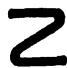
\includegraphics[keepaspectratio]{images/part002_2a386891d62f089ad1c0e080d8072868eea932699f46973e31691c72a41ba0df.jpg}}

``for all \(x \in E\) , \(f(x) \leqslant g(x)\) , and there

and not

\[
f (y) <   g (y) ^ {\prime \prime}
\]

\[
" \text { for   all } x \in \mathrm{E}, f (x) <   g (x)".
\]

In order to avoid confusion it is better not to use the notation \(f < g\) in this situation.

The definitions of this subsection apply without change to preordered sets when ``ordering'' is replaced by ``preordering'' throughout.

\subsection{INCREASING MAPPINGS}

DEFINITION 1. Let E and F be preordered sets (the preorder relation in each being denoted by \(\leqslant\) ). A mapping f of E into F is said to be increasing (or order-preserving) if the relation \(x \leqslant y\) implies \(f(x) \leqslant f(y)\) ; it is decreasing (or order-reversing) if the relation \(x \leqslant y\) implies \(f(x) \geqslant f(y)\) . A mapping of E into F is said to be monotone if it is either increasing or decreasing.

An increasing mapping of E into F becomes decreasing (and vice versa) when we replace one of the preorderings on E or on F by the opposite preordering. Every constant function is both increasing and decreasing; the converse of this statement is usually not true.

For example, if a set E is ordered by the equality relation, the identity mapping of E onto itself is both increasing and decreasing, but not constant if E has more than one element (cf.~Exercise 7).

DEFINITION 2. Let E and F be two ordered sets. A mapping f of E into F is said to be strictly increasing (or strictly order-preserving) if the relation x \textless{} y implies \(f(x) < f(y)\) ; f is said to be strictly decreasing (or strictly order-reversing) if the relation x \textless{} y implies \(f(x) > f(y)\) . A mapping of E into F is said to be strictly monotone if it is either strictly increasing or strictly decreasing.

Examples

\begin{enumerate}
\def\labelenumi{(\arabic{enumi})}
\item
  Let E be a set. The mapping \(X \rightarrow E - X\) of \(\mathfrak{P}(E)\) (ordered by inclusion) onto itself is strictly decreasing.
\item
  Let E be an ordered set. For each \(x \in E\) let \(U_x\) be the set of all \(y \in E\) such that \(y \geqslant x\) . The mapping \(x \to U_x\) is a strictly decreasing mapping of E into \(\mathfrak{P}(E)\) (ordered by inclusion); indeed, the relation \(x \leqslant y\) is equivalent to \(U_x \supset U_y\) .
\end{enumerate}

An injective monotone mapping of an ordered set E into an ordered set F is strictly monotone; the converse is usually not true, because it may happen that \(f(x) = f(y)\) when neither of the relations \(x \leqslant y\) , \(x \geqslant y\) is true (cf.~no. 12, Proposition 11).

A bijective mapping \(f\) of an ordered set \(\mathbf{E}\) onto an ordered set \(\mathbf{E}'\) is an isomorphism of \(\mathbf{E}\) onto \(\mathbf{E}'\) (no. 3) if and only if both \(f\) and its inverse mapping are increasing.

If I is an ordered index set, a family of subsets \((\mathbf{X}_t)_{i \in I}\) of a set E is said to be increasing if \(\iota \to \mathbf{X}_t\) is an increasing mapping of I into \(\mathfrak{P}(\mathbf{E})\) , ordered by inclusion (in other words, if \(\iota \leqslant x\) implies \(\mathbf{X}_t \subset \mathbf{X}_x\) ). Similarly we define a decreasing, strictly increasing, or strictly decreasing family of subsets \((\mathbf{X}_t)_{i \in I}\) .

PROPOSITION 2. Let E, E' be two ordered sets, and let u: E → E' and v: E' → E be two decreasing mappings such that for all x ∈ E and all x' ∈ E' we have v(u(x)) ≥ x and u(v(x')) ≥ x'. Then

\[
u \circ v \circ u = u \quad \text{and} \quad v \circ u \circ v = v.
\]

For the relation \(v(u(x)) \geqslant x\) implies \((u(v(u(x))) \leqslant u(x)\) because \(u\) is decreasing; on the other hand, we have \(u(v(u(x))) \geqslant u(x)\) by replacing \(x'\) by \(u(x)\) in the inequality \(u(v(x')) \geqslant x'\) . Hence the first equality; the proof of the second is similar.

\subsection{MAXIMAL AND MINIMAL ELEMENTS}

DEFINITION 3. Let E be an ordered set. An element \(a \in E\) is said to be a minimal (resp. maximal) element of E if the relation \(x \leqslant a\) (resp. \(x \geqslant a\) ) implies \(x = a\) .

Every minimal element of E is a maximal element with respect to the opposite ordering, and vice versa.

Examples

\begin{enumerate}
\def\labelenumi{(\arabic{enumi})}
\item
  Let A be a set. In the subset of \(\mathfrak{P}(A)\) (ordered by inclusion) consisting of the non-empty subsets of A, the minimal elements are the subsets consisting of a single element.
\item
  In the set \(\Phi(\mathbf{E},\mathbf{F})\) of mappings of subsets of \(\mathbf{E}\) into \(\mathbf{F}\) (F being non-empty), ordered by the relation '' \(v\) extends \(u\) '' between \(u\) and \(v\) , the maximal elements are the mappings of the whole of \(\mathbf{E}\) into \(\mathbf{F}\) .
\end{enumerate}

* (3) In the set of natural integers \textgreater{} 1, ordered by the relation ``m divides n'' between m and n, the minimal elements are the prime numbers. *

* (4) The set of real numbers has no maximal element and no minimal element. *

\subsection{GREATEST ELEMENT AND LEAST ELEMENT}

If there exists an element \(a\) in an ordered set \(\mathbf{E}\) such that \(a \leqslant x\) for all \(x \in \mathbf{E}\) , then \(a\) is the only element of \(\mathbf{E}\) with this property; for if also \(b \leqslant x\) for all \(x \in \mathbf{E}\) , then we should have \(a \leqslant b\) and \(b \leqslant a\) , and consequently \(a = b\) .

DEFINITION 4. Let E be an ordered set. An element \(a \in E\) is said to be the least (resp. greatest) element of E if for all \(x \in E\) we have \(a \leqslant x\) (resp. \(x \leqslant a\) ).

An ordered set need not have a greatest element nor a least element. If E has a least element a, then a is the greatest element with respect to the opposite ordering.

If E has a least element \(a\) , then \(a\) is the unique minimal element of E; for if \(x \in E\) is distinct from \(a\) , we have \(a < x\) .

Examples

\begin{enumerate}
\def\labelenumi{(\arabic{enumi})}
\item
  Let \(\mathfrak{S}\) be a non-empty subset of the set \(\mathfrak{P}(\mathbf{E})\) of subsets of a set \(\mathbf{E}\) . If \(\mathfrak{S}\) has a least (resp. greatest) element A with respect to the inclusion relation, then A is the intersection (resp. union) of the sets of \(\mathfrak{S}\) . Conversely, if the intersection (resp. union) of the sets of \(\mathfrak{S}\) belongs to \(\mathfrak{S}\) , then it is the least (resp. greatest) element of \(\mathfrak{S}\) .
\item
  In particular, \(\varnothing\) is the least element and E the greatest element of \(\mathfrak{P}(E)\) . In the set \(\Phi(E, F)\) of mappings of subsets of E into F, ordered by extension of mappings (no. 1, Example 3), the empty mapping is the least element, and there is no greatest element unless F consists of a single element. The diagonal \(\Delta\) of \(E \times E\) is the least element of the set of graphs of equivalence relations on E (or of the set of preorderings on E).
\end{enumerate}

PROPOSITION 3. Let E be an ordered set and let E' be the disjoint union of E and a set \{a\} consisting of a single element. Then there exists a unique ordering on E' which induces the given ordering on E and for which a is the greatest element of E'.

For if G is the graph of the ordering on E, the graph of an ordering on \(E'\) which satisfies the conditions of the Proposition must be the union \(G'\) of G and the set of all pairs \((x, a)\) where \(x \in E'\) ; conversely, it is clear that \(G'\) is the graph of an ordering on \(E'\) which satisfies the given conditions. ¶ The ordered set \(E'\) is said to be obtained by adjoining a greatest element a to E (cf.~Exercise 3).

A subset A of a preordered set E is said to be cofinal (resp. coinitial) in E if for every \(x \in E\) there exists \(y \in A\) such that \(x \leqslant y\) (resp. \(y \leqslant x\) ). To say that an ordered set E has a greatest (resp. least) element therefore means that E has a cofinal (resp. coinitial) subset consisting of a single element.

\subsection{UPPER AND LOWER BOUNDS}

DEFINITION 5. Let E be a preordered set and let X be a subset of E. Any element \(x \in \mathbf{E}\) such that \(x \leqslant y\) (resp. \(x \geqslant y\) ) for all \(y \in \mathbf{X}\) is called a lower (resp. upper) bound of X in E.

Every upper bound of X is a lower bound of X with respect to the opposite ordering, and vice versa.

If \(x\) is a lower bound of \(\mathbf{X}\) , every element \(z \leqslant x\) is also a lower bound of \(\mathbf{X}\) . A lower bound of \(\mathbf{X}\) is also a lower bound of every subset of \(\mathbf{X}\) . An ordered set \(\mathbf{X}\) has a least element if and only if there exists a lower bound of \(\mathbf{X}\) which belongs to \(\mathbf{X}\) .

The set of lower bounds of a subset X of a preordered set E may be empty: this is the case when X = E and E is an ordered set which has no least element.

A subset X of E whose set of lower (resp. upper) bounds is not empty is said to be bounded below (resp. bounded above). A subset which is bounded both below and above is said to be bounded. If X is bounded below (resp. bounded above, bounded), the same is true of every subset of X.

Every subset consisting of a single element is bounded. But a subset consisting of two elements need not be bounded either above or below (no. 10).

Let E be a preordered set and let f be a mapping of an arbitrary set A into E. The mapping f is said (by abuse of language) to be bounded below (resp. bounded above, bounded) if the set \(f(\mathbf{A})\) is bounded below (resp. bounded above, bounded) in E.

\subsection{LEAST UPPER BOUND AND GREATEST LOWER BOUND}

DEFINITION 6. Let E be an ordered set and let X be a subset of E. An element of E is said to be the greatest lower bound or infimum (resp. least upper bound or supremum) of X in E if it is the greatest (resp. least) element of the set of lower (resp. upper) bounds of X in E.

Given a subset X of an ordered set E, the least upper bound (resp. greatest lower bound) of X in E, when it exists, is denoted by

\[
\sup _ {\mathbf {E}} \mathbf {X} (\text { resp.   inf } _ {\mathbf {E}} \mathbf {X})
\]

or by sup X (resp. inf X) if there is no risk of ambiguity. The least upper bound (resp. greatest lower bound) of a set \(\{x, y\}\) of two elements, when it exists, is denoted by sup \((x, y)\) (resp. inf \((x, y)\) ). Similarly for the least upper bound and greatest lower bound of a set of three elements, etc. If a subset X of E has a greatest element a, then a is the least upper bound of X in E.

If X has a greatest lower bound \(a\) in E, then \(a\) is the least upper bound of X with respect to the opposite ordering on E. For this reason we may restrict ourselves for the most part, in what follows, to consideration of the properties of least upper bounds.

\minorheading{Examples}

\begin{enumerate}
\def\labelenumi{(\arabic{enumi})}
\item
  The set of upper bounds of the empty set \(\phi\) in an ordered set E is evidently E itself; hence \(\phi\) has a supremum in E if and only if E has a least element, which is then the least upper bound of \(\phi\) .
\item
  In the set \(\mathfrak{P}(\mathbf{E})\) of subsets of a set \(\mathbf{E}\) , ordered by inclusion, every subset \(\mathfrak{S}\) of \(\mathfrak{P}(\mathbf{E})\) has a least upper bound, namely the union of the sets of \(\mathfrak{S}\) , and a greatest lower bound, namely the intersection of the sets of \(\mathfrak{S}\) .
\item
  Let E, F be two sets and let \(\Theta\) be a subset of the \(\Phi(\mathbf{E}, \mathbf{F})\) of mappings of subsets of E into F, ordered by extension of mappings (no. 1, Example 3). For each \(u \in \Phi(\mathbf{E}, \mathbf{F})\) let \(\mathbf{D}(u)\) be the domain of u. The condition for the existence of a common extension of a family of mappings belonging to \(\Phi(\mathbf{E}, \mathbf{F})\) (Chapter II, § 4, no. 6, Proposition 7) shows that \(\Theta\) has a least upper bound in \(\Phi(\mathbf{E}, \mathbf{F})\) if and only if for each pair \((u, v)\) of elements of \(\Theta\) we have \(u(x) = v(x)\) whenever \(x \in \mathbf{D}(u) \cap \mathbf{D}(v)\) .
\end{enumerate}

A mapping \(f\) of a set \(A\) into an ordered set \(E\) is said to have a least upper bound if the image \(f(A)\) has a least upper bound in \(E\) ; this bound is then called the least upper bound of \(f\) and is written \(\sup_{x \in A} f(x)\) . Similarly for the greatest lower bound.

In particular, if a subset A of E has a least upper bound in E, this bound is the least upper bound of the canonical injection of A into E, and may therefore be written as sup x.

PROPOSITION 4. Let E be an ordered set and let A be a subset of E which has both a greatest lower bound and a least upper bound in E. Then inf A ≤ sup A if A ≠ ∅; if A = ∅, sup A is the least and inf A the greatest element of E.

This follows immediately from the definitions.

PROPOSITION 5. Let E be an ordered set and let A, B be two subsets of E, each of which has a least upper bound (resp. greatest lower bound) in E. If A ⊂ B, then sup A ≤sup B (resp. inf A ≥inf B).

COROLLARY. Let \((x_{t})_{i\in I}\) be a family of elements of an ordered set \(E\) which has a least upper bound in \(E\) . If \(J\) is a subset of \(I\) such that the family \((x_{t})_{i\in J}\) has a least upper bound in \(E\) , we have \(\sup_{i\in J}x_i\leqslant \sup_{i\in I}x_i\) .

PROPOSITION 6. Let \((x_{i})_{i\in I}, (y_{i})_{i\in I}\) be two families of elements of an ordered set E, indexed by the same set I, and such that \(x_{i} \leqslant y_{i}\) for all \(i\in I\) . If both families have a least upper bound in E, then \(\sup_{i\in I} x_{i} \leqslant \sup_{i\in I} y_{i}\) .

For \(a = \sup_{i \in I} y_i\) is an upper bound of the set of the \(y_i\) , so that \(x_i \leqslant y_i \leqslant a\) for all \(i \in I\) , and hence \(\sup_{i \in I} x_i \leqslant a\) .

PROPOSITION 7. Let \((x_{t})_{t\in I}\) be a family of elements of an ordered set \(E\) , and let \((J_{\lambda})_{\lambda \in I}\) be a covering of the index set \(I\) . Suppose that each of the subfamilies \((x_{t})_{t\in J_{\lambda}}\) has a least upper bound in \(E\) . For the family \((x_{t})_{t\in I}\) to have a least upper bound in \(E\) , it is necessary and sufficient that the family \(\left(\sup_{t\in J_{\lambda}}x_{t}\right)_{\lambda \in L}\) should have a least upper bound in \(E\) , and then we have

\[
\sup _ {i \in I} x _ {i} = \sup _ {\lambda \in L} \left(\sup _ {i \in J _ {\lambda}} x _ {i}\right).\tag{1}
\]

Let \(b_{\lambda} = \sup_{i \in J_{\lambda}} x_i\) . Suppose that \((x_i)_{i \in I}\) has a least upper bound \(a\) . Then \(a \geqslant b_{\lambda}\) for each \(\lambda \in L\) (Corollary to Proposition 5). On the other hand, if \(c \geqslant b_{\lambda}\) for each \(\lambda \in L\) , then we have \(c \geqslant x_i\) for each \(i \in I\) , because \((J_{\lambda})_{\lambda \in L}\) is a covering of \(I\) ; hence \(c \geqslant a\) , which proves that

\[
a = \sup _ {\lambda \in L} b _ {\lambda}.
\]

Conversely, suppose that the family \((b_{\lambda})_{\lambda \in \mathbf{L}}\) has a least upper bound \(a'\) . Then \(a' \geqslant x_{i}\) for all \(i \in I\) . On the other hand, if \(c' \geqslant x_{i}\) for all \(i \in I\) , then we have in particular

\[
c ^ {\prime} \geqslant \sup _ {i \in J _ {\lambda}} x _ {i} = b _ {\lambda}
\]

for each \(\lambda \in \mathbf{L}\) , so that \(c' \geqslant a'\) and therefore

\[
a ^ {\prime} = \sup _ {i \in I} x _ {i}.
\]

COROLLARY. Let \((x_{\lambda \mu})_{(\lambda, \mu) \in \mathbf{L} \times \mathbf{M}}\) be a ``double'' family of elements of an ordered set \(\mathbf{E}\) such that for each \(\mu \in \mathbf{M}\) the family \((x_{\lambda \mu})_{\lambda \in \mathbf{L}}\) has a least upper bound in \(\mathbf{E}\) . For the family \((x_{\lambda \mu})_{(\lambda, \mu) \in \mathbf{L} \times \mathbf{M}}\) to have a least upper bound in \(\mathbf{E}\) , it is necessary and sufficient that the family \(\left(\sup_{\lambda \in \mathbf{L}} x_{\lambda \mu}\right)_{\mu \in \mathbf{M}}\) should have a least

upper bound in E, and then we have

\[
\sup _ {(\lambda , \mu) \in L \times M} x _ {\lambda \mu} = \sup _ {\mu \in M} \left(\sup _ {\lambda \in L} x _ {\lambda \mu}\right).\tag{2}
\]

PROPOSITION 8. Let \((\mathbf{E}_t)_{t \in I}\) be a family of ordered sets. Let A be a subset of the product ordered set \(\mathbf{E} = \prod_{t \in I} \mathbf{E}_t\) , and let \(\mathbf{A}_t = \operatorname{pr}_t \mathbf{A}\) for each \(t \in I\) . For A to have a least upper bound in \(\mathbf{E}\) it is necessary and sufficient that, for each \(t \in I\) , \(\mathbf{A}_t\) should have a least upper bound in \(\mathbf{E}_t\) , and then we have

\[
\sup A = (\sup A _ {t}) _ {t \in I} = \left(\sup _ {x \in A} \operatorname{pr} _ {t} x\right) _ {t \in I}.
\]

Suppose that, for each \(t \in I\) , \(A_t\) has a least upper bound \(b_t\) in \(E_t\) . To say that \(c = (c_t)\) is an upper bound of \(A\) then means that \(c_t \geqslant b_t\) for each \(t \in I\) , hence \((b_t)_{t \in I}\) is an upper bound of \(A\) . Conversely, suppose that \(A\) has a least upper bound \(a = (a_t)_{t \in I}\) ; for each \(x \in I\) , \(a_x\) is an upper bound of \(A_x\) , because if \(x_x \in A_x\) , there exists \(x \in A\) such that \(pr_x x = x_x\) , by the definition of \(A_x\) ; on the other hand, if \(a_x'\) is an upper bound of \(A_x\) in \(E_x\) , the element \(c' = (c_t')_{t \in I}\) for which

\[
c _ {i} ^ {\prime} = a _ {i} \quad \text { for } \quad i \neq x \quad \text { and } \quad c _ {x} ^ {\prime} = a _ {x} ^ {\prime}
\]

is an upper bound of A; consequently \(c' \geqslant a\) and therefore \(a_{x}' \geqslant a_{z}\) ; hence \(a_{x}\) is the least upper bound of \(A_{x}\) in \(E_{x}\) .

\pandocbounded{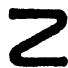
\includegraphics[keepaspectratio]{images/part002_f683a60c9eaa907b29b9c0e21fae4a1da7b4dd647e1d1a410962ae330fdaf4f4.jpg}}

Let F be a subset of an ordered set E, and let A be a subset of F. It can happen that one of the two elements \(\sup_{E} A\) , \(\sup_{F} A\) exists but the other does not, or that both exist but are unequal.

Examples

* (1) In the ordered set \(\mathbf{E} = \mathbf{R}\) of real numbers, consider the subset \(\mathbf{F} = \mathbf{Q}\) of rational numbers and the set \(\mathbf{A} \subset \mathbf{F}\) of rational numbers \(< \sqrt{2}\) ; \(\sup_{\mathbf{E}} \mathbf{A}\) exists but \(\sup_{\mathbf{F}} \mathbf{A}\) does not.

\begin{enumerate}
\def\labelenumi{(\arabic{enumi})}
\setcounter{enumi}{1}
\item
  In the notation of Example 1, let G be the union of A and the set \(\{2\}\) ; then \(G \subset F\) and \(\sup_{G} A\) exists, but \(\sup_{F} A\) does not.
\item
  With the same notation, \(\sup_{\mathbf{E}} \mathbf{A} = \sqrt{2}\) , \(\sup_{\mathbf{G}} \mathbf{A} = 2\) . *
\end{enumerate}

However, we have the following result :

PROPOSITION 9. Let E be an ordered set, F a subset of E, A a subset of F. If both \(\sup_{\mathbf{E}}\mathbf{A}\) and \(\sup_{\mathbf{F}}\mathbf{A}\) exist, we have \(\sup_{\mathbf{E}}\mathbf{A} \leqslant \sup_{\mathbf{F}}\mathbf{A}\) . If \(\sup_{\mathbf{E}}\mathbf{A}\) exists and belongs to F, then \(\sup_{\mathbf{F}}\mathbf{A}\) exists and is equal to \(\sup_{\mathbf{E}}\mathbf{A}\) .

The first assertion follows from the fact that the set M of upper bounds of A in F is contained in the set N of upper bounds of A in E, and from Proposition 5. On the other hand, if the least element of N lies in F, then it belongs to M and is clearly the least element of M; this proves the second assertion.

\subsection{DIRECTED SETS}

DEFINITION 7. A preordered set E is said to be right directed (resp. left directed) if every subset of two elements of E is bounded above (resp. bounded below).

In place of ``right directed'' we shall often use the expression ``directed with respect to the relation \(\leqslant\) '', and analogous expressions when the preorder relation is denoted by some other sign. For example, if S is a set of subsets of a set A, we say that S is directed with respect to the relation \(\subset\) (resp. \(\supset\) ) if, for each subset \(\{X, Y\}\) consisting of two elements of S, there exists \(Z \in S\) such that \(X \subset Z\) and \(Y \subset Z\) (resp. \(X \supset Z\) and \(Y \supset Z\) ).

Examples

\begin{enumerate}
\def\labelenumi{(\arabic{enumi})}
\tightlist
\item
  An ordered set which has a greatest element is right directed.
\end{enumerate}

* (2) In a topological space, a fundamental system of neighbourhoods of a point is directed with respect to the relation \(\supset\) .

\begin{enumerate}
\def\labelenumi{(\arabic{enumi})}
\setcounter{enumi}{2}
\tightlist
\item
  The set of submodules of finite type of an arbitrary module is directed with respect to the relation \(\subset\cdot_{*}\)
\end{enumerate}

PROPOSITION 10. In a right directed ordered set E, a maximal element \(a\) is the greatest element of E.

For every \(x \in \mathbf{E}\) there exists by hypothesis \(y \in \mathbf{E}\) such that \(x \leqslant y\) and \(a \leqslant y\) ; since \(a\) is maximal, \(y = a\) .

A right directed preordered set is left directed with respect to the opposite ordering. Any product of right directed sets is right directed. On the other hand, a subset of a right directed set is not necessarily right directed. However, a cofinal subset F of a right directed set E is always right directed; for given \(x, y \in \mathbf{F}\) there exists \(z \in \mathbf{E}\) such that \(x \leqslant z\) and \(y \leqslant z\) , and then \(t \in \mathbf{F}\) such that \(z \leqslant t\) .

\subsection{LATTICES}

DEFINITION 8. An ordered set E is said to be a lattice if every subset consisting of two elements of E has a least upper bound and a greatest lower bound in E.

Every product of lattices is a lattice; this follows from the condition for the existence of a least upper bound in a product of ordered sets (no. 9, Proposition 8). The set of subsets of a set A, ordered by inclusion, is a lattice because the union and intersection of two subsets of A are again subsets of A.

\minorheading{Examples}

* (1) The set of integers \(\geqslant 1\) , ordered by the relation `` \(m\) divides \(n\) '' between \(m\) and \(n\) , is a lattice; the least upper bound of \(\{m, n\}\) is the l.c.m. of \(m\) and \(n\) , and the greatest lower bound is their h.c.f.

\begin{enumerate}
\def\labelenumi{(\arabic{enumi})}
\setcounter{enumi}{1}
\item
  The set of subgroups of a group G, ordered by inclusion, is a lattice.
\item
  The set of topologies on a set A, ordered by the relation `` \(\mathfrak{G}\) is coarser than \(\mathfrak{G}'\)'' between \(\mathfrak{G}\) and \(\mathfrak{G}'\) , is a lattice. (General Topology, Chapter I, § 2).
\item
  The set \(\mathcal{F}(\mathbf{I},\mathbf{R})\) of all real-valued functions defined on an interval \(\mathbf{I}\) of \(\mathbf{R}\) is a lattice with respect to the order relation \(f\leqslant g\) (no. 4), and as such is isomorphic to the product \(\mathbf{R}^{\mathrm{I}}\) . *
\end{enumerate}

Remark. A lattice is obviously both left and right directed. But an ordered set which is both left and right directed is not necessarily a lattice. * An example of the latter is the set of mappings \(x \to p(x)\) of \(\mathbf{R}\) into itself, where \(p\) is a polynomial in \(\mathbf{R}[\mathbf{X}]\) , this set being ordered by the relation \(p \leqslant q\) (no. 4). *

\subsection{TOTALLY ORDERED SETS}

DEFINITION 9. Two elements \(x, y\) of a preordered set \(E\) are said to be comparable if the relation '' \(x \leqslant y\) or \(y \leqslant x\) '' is true. A set \(E\) is said to be totally ordered if it is ordered and if any two elements of \(E\) are comparable. The ordering on \(E\) is then said to be a total ordering, and the corresponding order relation a total order relation.

If \(x\) and \(y\) are elements of a totally ordered set, then \(x = y\) or \(x < y\) or \(x > y\) ; the negation of \(x \leqslant y\) is thus \(x > y\) .

An ordering on \(\mathbf{E}\) is a total ordering if and only if its graph \(\mathbf{G}\) satisfies the relation \(\mathbf{G} \cup \overline{\mathbf{G}} = \mathbf{E} \times \mathbf{E}\) , as well as the relations \(\mathbf{G} \circ \mathbf{G} = \mathbf{G}\) and \(\mathbf{G} \cap \overline{\mathbf{G}} = \Delta\) .

Examples

\begin{enumerate}
\def\labelenumi{(\arabic{enumi})}
\item
  Every subset of a totally ordered set is totally ordered by the induced ordering.
\item
  Let E be an arbitrary ordered set. The empty subset of E is totally ordered, and so is every subset of E consisting of a single element.
\end{enumerate}

* (3) The set \(\mathbf{R}\) of real numbers is totally ordered. *

\begin{enumerate}
\def\labelenumi{(\arabic{enumi})}
\setcounter{enumi}{3}
\tightlist
\item
  If A is a set which has at least two distinct elements, the set \(\mathfrak{P}(A)\) (ordered by inclusion) is not totally ordered, for if \(x \neq y\) , the subsets \(\{x\}\) and \(\{y\}\) are not comparable.
\end{enumerate}

A totally ordered set is also totally ordered with respect to the opposite ordering; it is a lattice and a fortiori both left and right directed.

PROPOSITION 11. Every strictly monotone mapping \(f\) of a totally ordered set \(\mathbf{E}\) into an ordered set \(\mathbf{F}\) is injective. If \(f\) is strictly increasing, \(f\) is an isomorphism of \(\mathbf{E}\) onto \(f(\mathbf{E})\) .

For \(x \neq y\) implies that either \(x < y\) or \(x > y\) ; hence

\[
f (x) <   f (y) \quad \text { or } \quad f (x) > f (y),
\]

so that \(f(x) \neq f(y)\) in either case. It remains to be shown that if \(f\) is strictly increasing, \(f(x) \leqslant f(y)\) implies \(x \leqslant y\) ; if not, we should have \(x > y\) , and therefore \(f(x) > f(y)\) .

PROPOSITION 12. Let E be a totally ordered set and let X be a subset of E. For an element b of E to be the least upper bound of X in E, it is necessary and sufficient that (1) b is an upper bound of X, (2) for every \(c \in E\) such that c \textless{} b, there exists \(x \in X\) such that \(c < x \leqslant b\) .

The second condition says that no element c \textless{} b is an upper bound of X, i.e., b is a minimal element of the set M of upper bounds of X; but this is the same as saying that b is the least element of M, since M is totally ordered (no. 10, Proposition 10).

\subsection{INTERVALS}

Let E be an ordered set and let a, b be two elements of E such that \(a \leqslant b\) . The subset of E consisting of elements x such that \(a \leqslant x \leqslant b\) is called the closed interval with left-hand endpoint a and right-hand endpoint b, and is denoted by {[}a, b{]}. The set of all \(x \in E\) such that \(a \leqslant x < b\) (resp. \(a < x \leqslant b\) ) is called the interval half-open on the right (resp. on the left) with endpoints a and b, and is denoted by {[}a, b{[} (resp. {]}a, b{]}). The set of all \(x \in E\) such that a \textless{} x \textless{} b is called the open interval with endpoints a and b, and is denoted by {]}a, b{[}.

Note that a closed interval is never empty; the interval \([a, a]\) is the set \(\{a\}\) . On the other hand, the intervals \([a, a[, ]a, a], ]a, a[\) are all empty; and an open interval \(]a, b[\) may be empty even when \(a < b\) .

Let \(a\) be an element of \(E\) . The set of all \(x \in E\) such that \(x \leqslant a\) (resp. \(x < a\) ) is called the closed (resp. open) interval unbounded on the left, with right-hand endpoint \(a\) , and is denoted by \(] \leftarrow, a]\) (resp. \(] \leftarrow, a[\) ); likewise, the set of all \(x \in E\) such that \(x \geqslant a\) (resp. \(x > a\) ) is called the closed (resp. open) interval with left-hand endpoint \(a\) , unbounded on the right, and is denoted by \([a, \leftarrow[\) (resp. \(]a, \leftarrow[\) ). Finally, \(E\) itself may be regarded as the open interval unbounded on the left and on the right, denoted by \(] \leftarrow, \rightarrow [.\)

PROPOSITION 13. In a lattice, the intersection of two intervals is an interval. Consider for example the intersection of two closed intervals \([a, b]\) and \([c, d]\) , and let \(\alpha = \sup (a, c)\) , \(\beta = \inf (b, d)\) . If both \(a \leqslant x \leqslant b\) and \(c \leqslant x \leqslant d\) , then we have \(\alpha \leqslant x \leqslant \beta\) , and conversely; if \(\alpha \not\leqslant \beta\) , the intersection of \([a, b]\) and \([c, d]\) is empty; if \(\alpha \leqslant \beta\) , this intersection is \([\alpha, \beta]\) . We leave it to the reader to carry through the proof for the other cases.

\section{WELL-ORDERED SETS}

\subsection{SEGMENTS OF A WELL-ORDERED SET}

A relation \(R\{x, y\}\) is said to be a well-ordering relation between x and y if R is an order relation between x and y and if, for each non-empty set E on which \(R\{x, y\}\) induces an order relation (i.e., such that \(x \in E\) implies \(R\{x, x\}\) ; cf.~§1, no. 1), E, ordered by this relation, has a least element.

A set E ordered by an ordering \(\Gamma\) is said to be well-ordered if the relation \(y \in \Gamma\langle x \rangle\) is a well-ordering relation between x and y; \(\Gamma\) is then said to be a well-ordering on E. The following definition is equivalent to this:

DEFINITION 1. A set E is said to be well-ordered if it is ordered and if each non-empty subset of E has a least element.

A well-ordered set E is totally ordered because every subset \(\{x, y\}\) of E has a least element. Every subset A of E which is bounded above in E has a least upper bound in E.

\minorheading{Examples}

\begin{enumerate}
\def\labelenumi{(\arabic{enumi})}
\item
  Let \(\mathbf{E} = \{\alpha, \beta\}\) be a set whose elements are distinct. It is easily verified that the subset \(\{(\alpha, \alpha), (\beta, \beta), (\alpha, \beta)\}\) of \(\mathbf{E} \times \mathbf{E}\) is the graph of a well-ordering on \(\mathbf{E}\) .
\item
  Every subset (in particular, the empty subset) of a well-ordered set is well-ordered by the induced ordering.
\end{enumerate}

* (3) The existence of totally ordered sets which are not well-ordered is equivalent to the axiom of infinity (§ 4, no. 4, Corollary 1 to Proposition 3, and Exercise 3).

\begin{enumerate}
\def\labelenumi{(\arabic{enumi})}
\setcounter{enumi}{3}
\item
  If \(\Gamma\) is a well-ordering on \(E\) , the ordering opposite to \(\Gamma\) is a well-ordering on \(E\) only if \(E\) is finite ( \(\S 4\) , Exercise 3). *
\item
  Let E be a well-ordered set. The set \(E_{1}\) obtained by adjoining to E a greatest element b (§1, no. 7) is well-ordered, for if H is any non-empty subset of \(E_{1}\) other than \(\{b\}\) , the least element of \(H \cap E\) is also the least element of H.
\end{enumerate}

Remark. * As a consequence of the axiom of infinity (§6, no. 1), there exist well-ordered sets which have no greatest element, for example the set N of natural integers. *

DEFINITION 2. In an ordered set E, a subset of E such that the relations \(x \in S\) , \(y \in E\) , and \(y \leqslant x\) imply \(y \in S\) is called a segment of E.

Clearly, every intersection and union of segments of E is a segment of E. If S is a segment of E, every segment of S is also a segment of E. The set E itself and the empty set are segments of E.

PROPOSITION 1. In a well-ordered set E, every segment of E other than E itself is an interval {]}←, a{[}, where a ∈ E.

Let S be a segment of E such that \(S \neq E\) . Since E --- S is not empty, it has a least element a. By virtue of Definition 2, the relation \(x \geqslant a\) implies \(x \notin S\) ; otherwise we would have \(a \in S\) , which is absurd. Hence E --- S is the interval \([a, \rightarrow[, \text{ and } S \text{ is the interval}] \leftarrow, a[\) .

For every element \(x\) in a totally ordered set \(\mathbf{E}\) the segment \(] \leftarrow, x[\) is called the segment with endpoint \(x\) , and is denoted by \(\mathbf{S}_x\) .

Note that if E is well-ordered and not empty, \(S_{x}\) has a least element \(\alpha\) and consequently is also the interval \([\alpha, x[\) .

Let E be a totally ordered set. The union A of the \(S_{x}\) , as x runs through E, is E if E has no greatest element; and if E has a greatest element b, we have \(A = E - \{b\}\) .

PROPOSITION 2. The set \(\mathbf{E}^*\) of segments of a well-ordered set \(\mathbf{E}\) is well-ordered by inclusion. The mapping \(x \to S_x\) is an isomorphism of the well-ordered set \(\mathbf{E}\) onto the set of segments of \(\mathbf{E}\) other than \(\mathbf{E}\) itself.

It is clear that if \(x \in \mathbf{E}\) and \(y \in \mathbf{E}\) , the relation \(x \leqslant y\) implies \(\mathrm{S}_x \subset \mathrm{S}_y\) , and that \(x < y\) implies \(\mathrm{S}_x \neq \mathrm{S}_y\) ; the mapping \(x \to \mathrm{S}_x\) is therefore an isomorphism of \(\mathbf{E}\) onto the set \(\mathrm{S}(\mathbf{E})\) of segments of \(\mathbf{E}\) distinct from \(\mathbf{E}\) itself (§ 1, no. 12, Proposition 11), and consequently \(\mathrm{S}(\mathbf{E})\) is well-ordered. Moreover, \(\mathbf{E}^*\) is isomorphic to the well-ordered set obtained from \(\mathrm{S}(\mathbf{E})\) by adjoining a greatest element.

PROPOSITION 3. Let \((\mathbf{X}_{\iota})_{\iota \in \mathbf{I}}\) be a family of well-ordered sets such that for each pair of indices \((\iota, \varkappa)\) one of the sets \(\mathbf{X}_{\iota}, \mathbf{X}_{\varkappa}\) is a segment of the other. Then there exists a unique ordering on the set \(\mathbf{E} = \bigcup_{\iota \in \mathbf{I}} \mathbf{X}_{\iota}\) which induces the given ordering on each of the \(\mathbf{X}_{\iota}\) . Endowed with this ordering, \(\mathbf{E}\) is a well-ordered set. Every segment of \(X_{t}\) is a segment of E; for each \(x \in X_{t}\) , the segment with endpoint x in \(X_{t}\) is equal to the segment with endpoint x in E; and each segment of E is either E itself or a segment of one of the \(X_{t}\) .

The first assertion is a consequence of the following general lemma :

LEMMA 1. Let \((\mathbf{X}_{\alpha})_{\alpha \in \Lambda}\) be a family of ordered sets, directed with respect to the relation \(c\) (in other words, such that for each pair of indices \(\alpha, \beta\) there exists an index \(\gamma\) such that \(\mathbf{X}_{\alpha} \subset \mathbf{X}_{\gamma}\) and \(\mathbf{X}_{\beta} \subset \mathbf{X}_{\gamma}\) ). Suppose that, for each pair of indices \((\alpha, \beta)\) such that \(\mathbf{X}_{\alpha} \subset \mathbf{X}_{\beta}\) , the ordering induced on \(\mathbf{X}_{\alpha}\) by that of \(\mathbf{X}_{\beta}\) is identical with the given ordering on \(\mathbf{X}_{\alpha}\) . Under these conditions there exists a unique ordering on the set \(\mathbf{E} = \bigcup_{\alpha \in \Lambda} \mathbf{X}_{\alpha}\) which induces the given ordering on each \(\mathbf{X}_{\alpha}\) .

Let \(G_{\alpha}\) be the graph of the given ordering on \(X_{\alpha}\) . If G is the graph of an ordering on E which induces on each \(X_{\alpha}\) the ordering whose graph is \(G_{\alpha}\) , then we must have \(G_{\alpha} \subset G\) for each \(\alpha \in A\) ; hence G contains \(\bigcup_{\alpha \in A} G_{\alpha}\) . On the other hand, for each pair \((x, y)\) of elements of E there exists by hypothesis an index \(\alpha \in A\) such that \(x \in X_{\alpha}\) and \(y \in X_{\alpha}\) ; if \((x, y) \in G\) , we have \((x, y) \in G_{\alpha}\) , so that \(G \subset \bigcup_{\alpha \in A} G_{\alpha}\) . Hence if the required ordering on E exists, its graph is necessarily \(G = \bigcup_{\alpha \in A} G_{\alpha}\) . It remains to be shown that this set satisfies the conditions of the lemma. Since \(G_{\beta} \cap (X_{\alpha} \times X_{\alpha}) = G_{\alpha}\) if \(X_{\alpha} \subset X_{\beta}\) , we have \(G \cap (X_{\alpha} \times X_{\alpha}) = G_{\alpha}\) for all \(\alpha \in A\) ; on the other hand, it follows from the hypothesis that any three elements \(x, y, z\) of E belong to the same \(X_{\alpha}\) . Hence \((x, y) \in G\) is an order relation on E, and the lemma is proved.

We now take up the proof of Proposition 3. Let us begin by showing that each \(\mathbf{X}_{\iota}\) is a segment of E. Indeed, if \(x \in \mathbf{X}_{\iota}, y \in \mathbf{E}\) , and \(y \leqslant x\) , there exists an index \(x\) such that \(\mathbf{X}_{\iota} \subset \mathbf{X}_{x}\) and \(y \in \mathbf{X}_{x}\) ; since by hypothesis \(\mathbf{X}_{\iota}\) is a segment of \(\mathbf{X}_{x}\) , we have \(y \in \mathbf{X}_{\iota}\) , which proves the assertion. The same reasoning proves that for each \(x \in \mathbf{X}_{\iota}\) the segment with endpoint \(x\) in \(\mathbf{X}_{\iota}\) is identical with the interval {]}←, \(x[\) in E. Next let us show that E is well-ordered. If H is a non-empty subset of E, there is an index \(\iota \in I\) such that \(\mathrm{H} \cap \mathrm{X}_{\iota} \neq \emptyset\) ; if \(a\) is the least element of \(\mathrm{H} \cap \mathrm{X}_{\iota}\) in \(\mathbf{X}_{\iota}\) , then \(a\) is also the least element of H in E. That is, if \(x \in H\) , there exists an index \(x \in I\) such that \(\mathbf{X}_{\iota} \subset \mathbf{X}_{x}\) and \(x \in \mathbf{X}_{x}\) ; we cannot have \(x < a\) , because the interval {]}←, \(a[\) is contained in \(\mathbf{X}_{\iota}\) , and therefore we have \(x \geqslant a\) since \(\mathbf{X}_{x}\) is totally ordered.

Finally, we must show that a segment of E, other than E itself, is a segment of one of the \(X_{t}\) ; this is an immediate consequence of the preceding arguments, since such a segment is of the form \(]\leftarrow\) , \(x[\text{(Proposition 1)}\) and since x belongs to some \(X_{t}\) .

\subsection{THE PRINCIPLE OF TRANSFINITE INDUCTION}

LEMMA 2. Let E be a well-ordered set and let S be a set of segments of E with the following properties: (1) every union of segments belonging to S belongs to S; (2) if \(S_{x} \in S\) , then \(S_{x} \cup \{x\} \in S\) . Then every segment of E belongs to S.

Suppose that there are segments of E which do not belong to S, and let S be the smallest of them (no. 1, Proposition 2). If S has no greatest element, then S is the union of the segments of S distinct from S itself, and these segments belong to S by virtue of the definition of S; hence \(S \in S\) , which is absurd. If, on the other hand, S has a greatest element a, then \(S = S_{a} \cup \{a\}\) , and since \(S_{a}\) is a segment of S distinct from S, we have \(S_{a} \in S\) ; but then also \(S \in S\) , which again is absurd.

For greater convenience we shall place ourselves in a theory \(\mathfrak{G}\) in which \(\mathbf{E}\) is a set well-ordered by a relation written \(x \leqslant y\) . We have then the following criteria:

C59. (Principle of transfinite induction). Let \(\mathbf{R}\{x\}\) be a relation in \(\mathfrak{G}\) ( \(x\) not being a constant of \(\mathfrak{G}\) ) such that the relation

\[
(x \in \mathrm{E} \text { and } (\forall y) ((y \in \mathrm{E} \text { and } y <   x) \Longrightarrow \mathrm{R} \{\left. y \right\})) \Longrightarrow \mathrm{R} \{x \}
\]

is a theorem in \(\mathfrak{G}\) . Under these conditions the relation \((x\in \mathbf{E})\Rightarrow \mathbb{R}\{x\}\) is a theorem in \(\mathfrak{G}\) .

Let \(\mathfrak{S}\) be the set of segments S of E such that \((y\in S)\Longrightarrow R\{y\}\) . It is clear that every union of segments belonging to \(\mathfrak{S}\) also belongs to \(\mathfrak{S}\) . On the other hand, if \(S_x\in \mathfrak{S}\) , we have \(R\{x\}\) by hypothesis; hence \((y\in S_x\cup \{y\})\Longrightarrow R\{y\}\) by the method of disjunction of cases. Hence (Lemma 2) \(E\in \mathfrak{S}\) , which proves the criterion.

In the applications of C59, the relation

\[
x \in \mathrm{E} \text {   and   } (\forall y) ((y \in \mathrm{E} \text {   and   } y <   x) \Longrightarrow \mathrm{R} \{y \})
\]

is usually called the ``inductive hypothesis''.

In what follows, for every mapping \(g\) of a segment \(S\) of \(E\) into a set \(F\) , and for each \(x \in S\) we shall denote by \(g^{(x)}\) the mapping of the segment \(S_x = ] \leftarrow, x[\) of \(E\) onto \(g(S_x)\) which coincides with \(g\) on \(S_x\) . With this notation we have

C60. (Definition of a mapping by transfinite induction.) Let \(u\) be a letter, \(T\{u\}\) a term in the theory \(\mathfrak{G}\) . There exists a set \(U\) and a mapping \(f\) of \(E\) onto \(U\) such that for all \(x \in E\) we have \(f(x) = T\{f^{(x)}\}\) . Furthermore, the set \(U\) and the mapping \(f\) are uniquely determined by these conditions.

Let us first prove the uniqueness. Suppose that \(f'\) and \(U'\) also satisfy the conditions of the criterion. Let \(\mathfrak{S}\) be the set of segments \(S\) of \(E\) such that \(f\) and \(f'\) coincide on \(S\) . It is clear that every union of segments belonging to \(\mathfrak{S}\) also belongs to \(\mathfrak{S}\) . On the other hand, if \(S_x \in \mathfrak{S}\) , then \(f\) and \(f'\) agree on \(S_x\) and therefore \(f^{(x)} = f'^{(x)}\) ; consequently

\[
f (x) = \mathrm{T} \left\{f ^ {(x)} \right\} = \mathrm{T} \left\{f ^ {\prime (x)} \right\} = f ^ {\prime} (x),
\]

which shows that \(\mathbf{S}_x\cup \{x\} \in \mathfrak{S}\) . It follows that \(\mathbf{E}\in \mathfrak{S}\) (Lemma 2), hence \(f^{\prime} = f\) and \(\mathbf{U}' = f'(\mathbf{E}) = f(\mathbf{E}) = \mathbf{U}\) .

Now let \(\mathfrak{S}_1\) denote the set of segments S of E for which there exists a set \(U_S\) and a mapping \(f_S\) of S onto \(U_S\) such that for all \(x \in S\) we have \(f_S(x) = T \{ f^{(x)} \}\) . For each \(S \in S_1\) , \(f_S\) and \(U_S\) are uniquely determined, by the first part of the proof; in particular, if \(S'\) and \(S''\) are two segments belonging to \(\mathfrak{S}_1\) such that \(S' \subset S''\) , then \(f_S'\) is the mapping of \(S'\) onto \(f_{S'}(S')\) which agrees with \(f_{S'}\) on \(S'\) . From this remark it follows that every union of segments belonging to \(\mathfrak{S}_1\) also belongs to \(\mathfrak{S}_1\) (Chapter II, §4, no. 6, Proposition 7). On the other hand, if \(S_x \in \mathfrak{S}_1\) , we define on \(S = S_x \cup \{x\}\) a function \(f_S\) extending \(f_{S_x}\) by putting

\[
f _ {\mathbf {S}} (x) = \mathrm{T} \left\{f _ {\mathbf {s} _ {x}} \right\}
\]

(Chapter II, § 4, no. 7, Proposition 8); since \(f_{\mathbb{S}}^{(x)} = f_{\mathbb{S}_x}\) , it is obvious that \(\mathbf{S}_x \cup \{x\} \in \mathfrak{S}_1\) . Hence (Lemma 2) \(\mathbf{E} \in \mathfrak{S}_1\) , and the proof is complete.

Usually this criterion is applied in situations where there exists a set F such that for every mapping h of a segment of E onto a subset of F we have \(T\{h\}\in F\) . Then the set U obtained by applying C60 is a subset of F. For, with the notation used above, let \(S_{2}\) be the subset of \(S_{1}\) consisting of segments S of E such that \(U_{S}\subset F\) . It is evident that every union of segments belonging to \(S_{2}\) also belongs to \(S_{2}\) ; on the other hand, the hypothesis on F implies that if \(S_{x}\in S_{2}\) , we have \(S_{x}\cup\{x\}\in S_{2}\) . The assertion now follows from Lemma 2.

\subsection{ZERMELO'S THEOREM}

LEMMA 3. Let E be a set, let S be a subset of \(\mathfrak{P}(\mathbf{E})\) , and let \(p\) be a mapping of S into E such that \(p(\mathbf{X}) \notin \mathbf{X}\) for all \(\mathbf{X} \in \mathfrak{S}\) . Then there exists a subset M of E and a well-ordering \(\Gamma\) on M such that, if \(x \leqslant y\) denotes the relation \(y \in \Gamma\langle x \rangle\) and \(\mathrm{S}_x\) denotes the segment {]}←, \(x]\) ,

\begin{enumerate}
\def\labelenumi{(\arabic{enumi})}
\item
  for all \(x \in \mathbf{M}\) we have \(\mathbf{S}_x \in \mathfrak{S}\) and \(p(\mathbf{S}_x) = x\) ;
\item
  \(\mathbf{M} \notin \mathfrak{S}\) .
\end{enumerate}

Let \(\mathfrak{M}\) be the set of subsets \(\mathbf{G}\) of \(\mathbf{E} \times \mathbf{E}\) satisfying the following conditions:

\begin{enumerate}
\def\labelenumi{(\alph{enumi})}
\item
  \(\mathbf{G}\) is the graph of a well-ordering on \(\mathbf{pr}_1\mathbf{G} = \mathbf{U}\) ;
\item
  if \(x \leqslant y\) denotes the relation \((x, y) \in \mathbf{G}\) on \(\mathbf{U}\) , then for each \(x \in \mathbf{U}\) the segment \(S_x\) is such that \(S_x \in \mathfrak{S}\) and \(p(S_x) = x\) . We shall show that if \(G\) and \(G'\) are two elements of \(M\) and if \(U, U'\) denote their first projections, then one of the two sets \(U, U'\) is contained in the other and that if, for example, \(U \subset U'\) , then \(G = G' \cap (U \times U)\) (in other words, that the order relation on \(U\) is induced by the order relation on \(U'\) ) and \(U\) is a segment of \(U'\) .
\end{enumerate}

Consider the set V of elements \(x \in U \cap U'\) such that the segments with endpoint x are the same in U and \(U'\) , and such that the orderings induced on this segment by the orderings on U and \(U'\) are identical. It is clear that V is a segment in both U and \(U'\) and that the orderings induced on V are the same; our assertion will therefore be proved if we show that either V = U or \(V = U'\) . Let us argue by contradiction and suppose that \(V \neq U\) and \(V \neq U'\) . Let x be the least element of U - V in U and let \(x'\) be the least element of \(U' - V\) in \(U'\) ; we have \(V = S_x\) in U, and \(V = S_x'\) in \(U'\) . But by hypothesis, \(V \in S\) and

\[
x = p \left(\mathrm{S} _ {x}\right), \quad x ^ {\prime} = p \left(\mathrm{S} _ {x ^ {\prime}}\right),
\]

so that \(x = x'\) . Hence by definition \(x \in V\) , which is absurd. We may therefore apply Proposition 3 of no. 1 to the set of first projections \(U = pr_1G\) (where \(G \in \mathfrak{M}\) ) and thus obtain a well-ordered set

\[
\mathrm{M} = \bigcup_ {\mathrm{G} \in \mathfrak {M}} \operatorname{pr} _ {1} \mathrm{G}.
\]

It is easily seen that the graph of the ordering on M belongs to M. If we had \(M \in S\) , then, putting \(a = p(M)\) , we should have \(a \notin M\) . We could therefore adjoin to M the element a as greatest element, and the set \(M' = M \cup \{a\}\) would be well-ordered. Since \(M = S_a\) in \(M'\) , we should have \(S_a \in S\) and \(p(S_a) = a\) ; the graph of the ordering on \(M'\) would therefore belong to M, which is absurd.

Note that if \(\phi \notin \mathfrak{S}\) (and in particular if \(\mathfrak{S}\) is empty), the set M whose existence is asserted by Lemma 3 is the empty set; this follows from condition 1 of Lemma 3.

\textbf{THEOREM 1 (Zermelo). Every set E can be well-ordered.}

Let \(\mathfrak{S} = \mathfrak{P}(\mathrm{E}) - \{\mathrm{E}\}\) be the set of all subsets of \(\mathbf{E}\) other than \(\mathbf{E}\) itself. For each \(\mathbf{X} \in \mathfrak{S}\) let \(p(\mathbf{X}) = \tau_x\) ( \(x \in \mathbf{E} - \mathbf{X}\) ); since the relation \(\mathbf{X} \in \mathfrak{S}\) implies \((\exists x)(x \in \mathbf{E} - \mathbf{X})\) , we have \(p(\mathbf{X}) \in \mathbf{E} - \mathbf{X}\) (Chapter I, §4, no. 1) and therefore \(p(\mathbf{X}) \notin \mathbf{X}\) . We may therefore apply Lemma 3, and consequently there exists a well-ordering on a subset \(\mathbf{M}\) of \(\mathbf{E}\) such that \(\mathbf{M} \notin \mathfrak{S}\) ; but the only subset of \(\mathbf{E}\) which does not belong to \(\mathfrak{S}\) is \(\mathbf{E}\) itself, and the theorem is proved.

\subsection{INDUCTIVE SETS}

DEFINITION 3. An ordered set E is said to be inductive if every totally ordered subset of E has an upper bound in E.

\minorheading{Examples}

\begin{enumerate}
\def\labelenumi{(\arabic{enumi})}
\item
  Let \(\mathfrak{F}\) be a set of subsets of a set \(A\) , ordered by inclusion, and such that for every totally ordered subset \(\mathfrak{G}\) of \(\mathfrak{F}\) the union of the sets of \(\mathfrak{G}\) belongs to \(\mathfrak{F}\) . Then \(\mathfrak{F}\) is inductive with respect to the relation \(\subset\) because the union of the sets of \(\mathfrak{G}\) is the least upper bound of \(\mathfrak{G}\) in \(\mathfrak{P}(A)\) .
\item
  An important example of a set of subsets which is inductive with respect to the relation \(\subset\) is the set \(\mathfrak{F}\) of graphs of mappings of subsets of a set A into a set B. For \(\mathfrak{F}\) is a subset of \(\mathfrak{P}(A \times B)\) , and to say that a subset \(\mathfrak{G}\) of \(\mathfrak{F}\) is totally ordered by inclusion means that the elements of \(\mathfrak{G}\) are graphs of mappings such that, given any two of these mappings, one is an extension of the other. It follows immediately that the union of the sets of \(\mathfrak{G}\) is an element of \(\mathfrak{F}\) (Chapter II, § 4, no. 6, Proposition 7). Hence the set \(\Phi(A, B)\) of mappings of subsets of A into B is inductive with respect to the order relation `` \(v\) extends \(u\) '' between \(u\) and \(v\) .
\end{enumerate}

* (3) It follows from the axiom of infinity (§ 6, no. 1) that the well-ordered set of natural integers is not inductive with respect to the relation ≤. *

THEOREM 2 (``Zorn's lemma''). Every inductive ordered set has a maximal element.

This theorem is a particular case of the following result :

PROPOSITION 4. Let E be an ordered set in which every well-ordered subset is bounded above; then E has a maximal element.

We shall say that an element \(v \in E\) is a strict upper bound of a subset \(X\) of \(E\) if \(v\) is an upper bound of \(X\) and \(v \notin X\) . Let \(\mathfrak{S}\) be the set of subsets of \(E\) which have a strict upper bound in \(E\) , and for each \(S \in \mathfrak{S}\) put \(p(S) = \tau_v(v\) is a strict upper bound of \(S)\) ; then \(p(S)\) is a strict upper bound of \(S\) . Applying Lemma 3 of no. 3 to \(\mathfrak{S}\) and \(p\) , we see that there exists a subset \(M\) of \(E\) and a well-ordering \(\Gamma\) on \(M\) which satisfies the conditions of Lemma 3; in particular, M has no strict upper bound in E. Furthermore, the ordering \(\Gamma\) is identical with that induced on M by the ordering on E. For in M the relation `` \(y \in \Gamma\langle x \rangle\) and \(x \neq y\) '' is equivalent to \(x \in S_y\) ; and since \(p(S_y) = y\) is an upper bound of \(S_y\) (with respect to the ordering on E), it implies \(x < y\) in E. But this means that the injection of M into E is a strictly increasing mapping (M being endowed with the ordering \(\Gamma\) ); and since M is totally ordered, it follows that the relations \(y \in \Gamma\langle x \rangle\) and \(x \leqslant y\) are equivalent in M ( \(\S 1\) , no. 12, Proposition 11). This being so, there exists by hypothesis an upper bound \(m\) of M in E; but since M has no strict upper bound, it follows that \(m\) is a maximal element of E.

COROLLARY 1. Let E be an inductive ordered set and let a be an element of E. Then there exists a maximal element m of E such that \(m \geqslant a\) .

For it follows from Definition 3 that the set F of elements \(x \geqslant a\) in E is inductive, and a maximal element of F is also maximal in E.

COROLLARY 2. Let \(\mathfrak{F}\) be a set of subsets of a set E such that, for every subset \(\mathfrak{G}\) of \(\mathfrak{F}\) which is totally ordered by inclusion, the union (resp. intersection) of the sets of \(\mathfrak{G}\) belongs to \(\mathfrak{F}\) ; then \(\mathfrak{F}\) has a maximal (resp. minimal) element.

\subsection{ISOMORPHISMS OF WELL-ORDERED SETS}

THEOREM 3. Let E and F be two well-ordered sets. Then at least one of the following two statements is true:

\begin{enumerate}
\def\labelenumi{(\arabic{enumi})}
\item
  there exists a unique isomorphism of \(\mathbf{E}\) onto a segment of \(\mathbf{F}\) ;
\item
  there exists a unique isomorphism of \(\mathbf{F}\) onto a segment of \(\mathbf{E}\) .
\end{enumerate}

Let \(\mathfrak{F}\) be the set of mappings of subsets of E into F such that each mapping is defined on a segment of E and is an isomorphism of this segment onto a segment of F. Then the set \(\mathfrak{F}\) , ordered by the relation `` \(v\) extends \(u\) '' between \(u\) and \(v\) , is inductive. For if \(\mathfrak{G}\) is a totally ordered subset of \(\mathfrak{F}\) , the union S of the domains of the mappings \(u \in \mathfrak{G}\) is a union of segments of E and is therefore itself a segment of E. If \(v\) is the least upper bound of \(\mathfrak{G}\) in \(\Phi(E, F)\) (no. 4, Example 2), then \(v(S)\) is the union of the ranges of the mappings \(u \in \mathfrak{G}\) and is therefore a segment of F. Finally, for each pair of elements \(x\) , \(y\) of S such that \(x < y\) there exists \(u \in \mathfrak{G}\) whose domain contains both \(x\) and \(y\) (because \(\mathfrak{G}\) is totally ordered); and since \(v(x) = u(x) < u(y) = v(y)\) , \(v\) is an isomorphism of S onto \(v(S)\) , and our assertion is proved.

Now let \(u_0\) be a maximal element of \(\mathfrak{F}\) (no. 4, Theorem 2) and let \(S_0\) be the segment of \(E\) which is the domain of \(u_0\) . If we show that either \(S_0 = E\) or \(u_0(S_0) = F\) , the theorem will be proved. Let us argue by contradiction and suppose that \(S_0 \neq E\) and \(u_0(S_0) \neq F\) . There will then be an element \(a \in E\) and an element \(b \in F\) such that \(S_0 = ]\leftarrow, a[\) and \(u_0(S_0) = ]\leftarrow, b[\) (no. 1, Proposition 1). Extend \(u_0\) to a mapping \(u_1\) of the segment \(]\leftarrow, a]\) into \(F\) by putting \(u_1(a) = b\) ; since \(u_1\) is an isomorphism of \(]\leftarrow, a]\) onto the segment \(]\leftarrow, b]\) , this contradicts the maximality of \(u_0\) in \(\mathfrak{F}\) .

The uniqueness asserted in Theorem 3 is a consequence of the following Lemma :

LEMMA 4. Let E, F be two well-ordered sets and let f, g be two increasing mappings of E into F such that \(f(\mathbf{E})\) is a segment of F and g is strictly increasing; then \(f(x) \leqslant g(x)\) for all \(x \in E\) .

Suppose, on the contrary, that the set of elements \(y \in E\) such that \(f(y) > g(y)\) is not empty; then this set will have a least element \(a\) . If \(x < a\) , we have then \(f(x) \leqslant g(x) < g(a) < f(a)\) since \(g\) is strictly increasing. Since \(f(E)\) is a segment of \(F\) , there exists \(z \in E\) such that \(g(a) = f(z)\) ; \(f\) is increasing, so that \(f(z) < f(a)\) implies \(z < a\) . Hence

\[
f (z) \leqslant g (z) <   g (a) = f (z),
\]

which is absurd.

COROLLARY 1. The only isomorphism of a well-ordered set E onto a segment of E is the identity mapping of E onto itself.

Put \(\mathbf{F} = \mathbf{E}\) in Theorem 3.

COROLLARY 2. Let E, F be two well-ordered sets. If there exists an isomorphism f of E onto a segment T of F and an isomorphism g of F onto a segment S of E, then we must have S = E, T = F, and g, f are inverses of each other.

For \(g \circ f\) is an isomorphism of \(\mathbf{E}\) onto the segment \(g(\mathbf{T}) \subset \mathbf{S}\) of \(\mathbf{E}\) ; by Corollary 1 we have \(g(\mathbf{T}) = \mathbf{S} = \mathbf{E}\) , and \(g \circ f\) is the identity mapping of \(\mathbf{E}\) . Similarly, \(f \circ g\) is the identity mapping of \(\mathbf{F}\) , whence the result.

COROLLARY 3. Every subset A of a well-ordered set E is isomorphic to a segment of E.

By virtue of Theorem 3 it is enough to prove that there exists no isomorphism g of E onto a segment of A of the form \(S_{a}\) . If there were, g would then be a strictly increasing mapping of E into E such that \(g(a) \in S_{a}\) , in other words such that \(g(a) < a\) ; but this inequality contradicts Lemma 4 (with f as the identity mapping).

\subsection{LEXICOGRAPHIC PRODUCTS}

Let \((\mathbf{E}_t)_{i\in I}\) be a family of ordered sets, indexed by a well-ordered set \(I\) . Consider the product set \(\mathbf{E} = \prod_{i\in I}\mathbf{E}_t\) and the relation

`` \(x \in E\) and \(y \in E\) , and for the least index \(t \in I\) such that \(\mathrm{pr}_t x \neq \mathrm{pr}_t y\) , we have \(\mathrm{pr}_t x < \mathrm{pr}_t y\) '',

which we shall denote by \(\mathbf{R}\{x, y\}\) . It is evident that \(\mathbf{R}\{x, x\}\) is equivalent to \(x \in \mathbf{E}\) , that \(\mathbf{R}\{x, y\}\) implies \(\mathbf{R}\{x, x\}\) and \(\mathbf{R}\{y, y\}\) , and that \((\mathbf{R}\{x, y\}\) and \(\mathbf{R}\{y, x\})\) implies \(x = y\) . Also it is easily verified that \((\mathbf{R}\{x, y\}\) and \(\mathbf{R}\{y, z\})\) implies \(\mathbf{R}\{x, z\}\) (consider the least index \(t \in I\) for which at least two of the three elements \(\mathrm{pr}_t x\) , \(\mathrm{pr}_t y\) , \(\mathrm{pr}_t z\) are unequal); hence \(\mathbf{R}\{x, y\}\) is an order relation on the product set E. This relation and the ordering it defines are called the lexicographic order relation and the lexicographic ordering on E (induced by the given orderings on I and on the \(\mathbf{E}_t\) ); the set E with this ordering is called the lexicographic product of the family of ordered sets \((\mathbf{E}_t)_{t \in I}\) . If each \(\mathbf{E}_t\) is totally ordere'd the lexicographic product is also totally ordered.

\section{EQUIPOTENT SETS. CARDINALS}

\subsection{THE CARDINAL OF A SET}

DEFINITION 1. A set X is said to be equipotent to a set Y if there exists a bijection of X onto Y. The relation ``X is equipotent to Y'' is denoted by Eq(X, Y).

The relations Eq(X, Y) and Eq(Y, X) are clearly equivalent, so that the relation Eq(X, Y) is symmetric; when it is true, we say that X and Y are equipotent. Next, Eq(X, X) is true. Finally, the relation Eq(X, Y) is transitive since the composition of two bijections is a bijection (Chapter II, §3, no. 8, Theorem 1); it is therefore an equivalence relation, reflexive on every set.

From what has been said it follows that if X and Y are equipotent, the relation

\[
(\forall \mathbf {Z}) (\operatorname{Eq} (\mathbf {X}, \mathbf {Z}) \Longleftrightarrow \operatorname{Eq} (\mathbf {Y}, \mathbf {Z}))
\]

is true. Now the axiom scheme S7 (Chapter I, §5, no. 1) gives us the following axiom :

\[
((\forall Z) (\operatorname{Eq} (X, Z) \Longleftrightarrow \operatorname{Eq} (Y, Z)) \Longrightarrow (\tau_ {Z} (\operatorname{Eq} (X, Z)) = \tau_ {Z} (\operatorname{Eq} (Y, Z))).
\]

Hence, if X and Y are equipotent, we have

\[
\tau_ {z} (\operatorname{Eq} (X, Z)) = \tau_ {z} (\operatorname{Eq} (Y, Z)),
\]

which justifies the following definition :

DEFINITION 2. The set \(\tau_{\mathbf{Z}}(\operatorname{Eq}(\mathbf{X},\mathbf{Z}))\) is called the cardinal of \(\mathbf{X}\) (or the power of \(\mathbf{X}\) ) and is written \(\operatorname{Card}(\mathbf{X})\) .

Since Eq(X, X) is true, Card(X) is equipotent to X (Chapter I, §4, Scheme S5). We have therefore proved the following result:

PROPOSITION 1. Two sets X and Y are equipotent if and only if their cardinals are equal.

\minorheading{Examples}

\begin{enumerate}
\def\labelenumi{(\arabic{enumi})}
\item
  \(\operatorname{Card}(\phi)\) is denoted by 0. Since the only set equipotent to \(\phi\) is \(\phi\) (Chapter II, §3, nos. 1 and 4), we have \(0 = \operatorname{Card}(\phi) = \phi\) .
\item
  All sets consisting of a single element are equipotent, since \(\{(a, b)\}\) is the graph of a bijection of \(\{a\}\) onto \(\{b\}\) ; in particular, they are all equipotent to \(\{\varnothing\}\) . The cardinal \(\operatorname{Card}(\{\varnothing\}) = \tau_{\mathbf{Z}}(\operatorname{Eq}(\{\varnothing\}, \mathbf{Z}))\) is denoted by 1. (*)
\item
  \(\operatorname{Card}(\{\varnothing, \{\varnothing\}\})\) is denoted by 2; this is the cardinal of every set consisting of two distinct elements.
\end{enumerate}

*(4) A Hilbert space of countable type is equipotent to the set of real numbers. *

\subsection{ORDER RELATION BETWEEN CARDINALS}

The relation ``X is equipotent to a subset of Y'' is equivalent to ``there exists an injection of X into Y''; it is also equivalent to the relation ``Card (X) is equipotent to a subset of Card (Y)'' (Chapter II, § 3, no. 8, Theorem 1).

THEOREM 1. The relation \(R\{\mathfrak{x}, \mathfrak{y}\}\) : `` \(\mathfrak{x}\) and \(\mathfrak{y}\) are cardinals and \(\mathfrak{x}\) is equipotent to a subset of \(\mathfrak{y}\) '' is a well-ordering relation (§2, no. 1).

Since \(\mathbf{R}\{\mathfrak{x},\mathfrak{x}\}\) is true for every cardinal \(\mathfrak{x}\) , what must be proved is that, for every set \(\mathbf{E}\) of cardinals the relation `` \(\mathfrak{x} \in \mathbf{E}\) and \(\mathfrak{y} \in \mathbf{E}\) and \(\mathbf{R}\{\mathfrak{x},\mathfrak{y}\}\) '' is a well-ordering relation on \(\mathbf{E}\) . Consider the set \(\mathbf{A} = \bigcup_{\mathfrak{r}\in \mathbf{E}}\mathfrak{x}\) .

Every cardinal \(\mathfrak{r} \in \mathbf{E}\) is then a subset of A. By §2, Theorem 1 there exists a well-ordering relation on A, which we shall denote by \(\mathfrak{r} \leqslant y\) , and every subset of A is equipotent to a segment of A (§2, no. 5, Theorem 3, Corollary \(x\) ). For every cardinal \(\mathfrak{r} \in \mathbf{E}\) consider the set of segments of A which are equipotent to \(\mathfrak{r}\) ; this set of segments is not empty and therefore has a least element (§2, no. 1, Proposition 2); let \(\varphi(\mathfrak{r})\) denote this least element. The relation

`` \(x \in E\) and \(y \in E\) and \(x\) is equipotent to a subset of \(y\) ''

is then equivalent to

\[
" \mathfrak {x} \in \mathrm{E} \text {   and   } \mathfrak {y} \in \mathrm{E} \text {   and   } \varphi (\mathfrak {x}) \subset \varphi (\mathfrak {y})".
\]

For clearly the second relation implies the first. Conversely, if \(\mathfrak{r}\) is equipotent to a subset of \(\varphi(\mathfrak{y})\) , we cannot have \(\varphi(\mathfrak{y}) \subset \varphi(\mathfrak{x})\) and \(\varphi(\mathfrak{y}) \neq \varphi(\mathfrak{x})\) ; otherwise there would exist a segment of \(\varphi(\mathfrak{y})\) equipotent to \(\mathcal{X}\) ( \(\S\) 2, no. 5, Theorem 3, Corollary 3), contrary to the definition of \(\varphi(\mathfrak{x})\) . Since the set of segments of A is well-ordered by inclusion ( \(\S\) 2, no. 1, Proposition 2), the theorem follows.

We shall denote the relation \(\mathbf{R}\{\mathfrak{x},\mathfrak{y}\}\) by \(\mathfrak{x}\leqslant \mathfrak{y}\) . A set \(\mathbf{X}\) is equipotent to a subset of a set \(\mathbf{Y}\) if and only if \(\operatorname{Card}(\mathbf{X})\leqslant \operatorname{Card}(\mathbf{Y})\) .

Clearly we have \(0 \leqslant \mathfrak{r}\) for every cardinal \(\mathfrak{r}\) , and \(1 \leqslant \mathfrak{r}\) for every cardinal \(\mathfrak{r} \neq 0\) .

COROLLARY 1. Given any two sets, one of them is equipotent to a subset of the other.

COROLLARY 2. Two sets each of which is equipotent to a subset of the other are equipotent.

Remark. Given any set A, there exists a set whose elements are the cardinals \(\operatorname{Card}(X)\) for all the subsets X of A, namely, the set of objects of the form \(\operatorname{Card}(X)\) for \(X \in \mathfrak{P}(A)\) (Chapter II, §1, no. 6). For every cardinal a the relation ``r is a cardinal and \(r \leqslant a\) '' is therefore collectivizing in r (Chapter II, §1, no. 4), because it is equivalent to the relation `` \(\mathfrak{f}\) is of the form Card (X) for \(X \subset \mathfrak{a}\) ''; the set of all \(\mathfrak{f}\) satisfying this relation is called the set of cardinals \(\leqslant \mathfrak{a}\) .

PROPOSITION 2. For every family \((\mathfrak{a}_i)_{i\in I}\) of cardinals, there exists a unique cardinal \(\mathfrak{b}\) such that \(\mathfrak{a}_i\leqslant \mathfrak{b}\) for all \(i\in I\) and such that every cardinal \(\mathfrak{c}\) for which \(\mathfrak{a}_i\leqslant \mathfrak{c}\) for all \(i\in I\) is \(\geqslant \mathfrak{b}\) .

There exists a set E containing all the sets \(a_{i}\) (e.g., the sum of these sets (Chapter II, §4, no. 8)), whence \(a_{i} \leqslant a = Card(E)\) for all \(i \in I\) . The set F of cardinals \(\leqslant a\) is well-ordered and contains all the \(a_{i}\) , and therefore the family \((a_{i})_{i \in I}\) has a least upper bound b in F. Let c be a cardinal \(\geqslant a_{i}\) for all \(i \in I\) ; if \(c < b \leqslant a\) , then \(c \in F\) , and the inequality \(a_{i} \leqslant c\) contradicts the definition of the least upper bound of the family \((a_{i})\) in the ordered set F; hence the result.

By abuse of language, the cardinal \(\mathfrak{b}\) is called the least upper bound of the family \((\mathfrak{a}_i)_{i\in I}\) and is denoted by \(\sup_{i\in I}a_i\) .

PROPOSITION 3. Let X and Y be sets. If there exists a surjection f of X onto Y, then Card (Y) ≤ Card (X).

For there exists a section \(s\) associated with \(f\) (Chapter II, §3, no. 8, Proposition 8) and \(s\) is an injection of Y into X.

\subsection{OPERATIONS ON CARDINALS}

DEFINITION 3. Let \((\mathfrak{a}_t)_{t \in I}\) be a family of cardinals. The cardinal of the product (resp. sum) of the sets \(\mathfrak{a}_t\) is called the cardinal product (resp. cardinal sum) of the cardinals \(\mathfrak{a}_t\) and is denoted by \(\underset{i \in I}{\mathsf{P}} \mathfrak{a}_t\) ( \(\text{resp. } \sum_{i \in I} \mathfrak{a}_t\) ).

Whenever there is no risk of confusion we shall say simply ``product'' and ``sum'' in place of ``cardinal product'' and ``cardinal sum'', and we shall write \(\prod_{i\in I}a_{i}\) in place of \(P_{i\in I}a_{i}\) (cf.~Exercise 2).

PROPOSITION 4. Let \((\mathbf{E}_t)_{i \in I}\) be a family of sets, P their product, and S their sum, and let \(a_t\) be the cardinal of \(\mathbf{E}_t\) . Then the cardinal of P (resp. S) is the cardinal product (resp. cardinal sum) of the family \((a_t)_{i \in I}\) .

For there exists a bijection of P (resp. S) onto the product (resp. sum) of the sets \((\mathfrak{a}_{t})\) (Chapter II, § 4, no. 8, Proposition 10, and § 5, no. 7, Corollary to Proposition 11).

COROLLARY. If \((\mathbf{E}_{t})_{t\in\mathbf{I}}\) is any family of sets, the cardinal of the union \(\bigcup_{t\in I}E_{t}\) is at most equal to the sum \(\sum\) Card \((\mathbf{E}_{t})\) .

For there exists a mapping of the sum S of the \(E_{t}\) onto the union of the \(E_{t}\) (Chapter II, §4, no. 8); the Corollary therefore follows from Propositions 3 and 4.

PROPOSITION 5. (a) Let \((\mathfrak{a}_i)_{i\in I}\) be a family of cardinals, and let \(f\) be a bijection of a set \(\mathbf{K}\) onto the index set \(\mathbf{I}\) . Then

\[
\sum_ {x \in \mathbb {K}} a _ {f (x)} = \sum_ {i \in I} a _ {i}, \quad \underset {x \in \mathbb {K}} {\mathsf {P}} a _ {f (x)} = \underset {i \in I} {\mathsf {P}} a _ {i}.
\]

\begin{enumerate}
\def\labelenumi{(\alph{enumi})}
\setcounter{enumi}{1}
\tightlist
\item
  Let \((\mathfrak{a}_t)_{t\in \mathbf{I}}\) be a family of cardinals and let \((\mathrm{J}_{\lambda})_{\lambda \in \mathbf{L}}\) be a partition of \(\mathbf{I}\) . Then
\end{enumerate}

\[
\sum_ {i \in I} a _ {i} = \sum_ {\lambda \in L} \left(\sum_ {i \in J _ {\lambda}} a _ {i}\right), \quad P _ {i \in I} a _ {i} = P _ {\lambda \in L} \left(P _ {i \in J _ {\lambda}} a _ {i}\right)
\]

(``associativity of the sum and product'').

\begin{enumerate}
\def\labelenumi{(\alph{enumi})}
\setcounter{enumi}{2}
\tightlist
\item
  Let \(((\mathfrak{a}_{\lambda t})_{t\in J_{\lambda}}\lambda \in L\) be a family (indexed by L) of families of cardinals, and let \(I = \prod_{\lambda \in I}J_{\lambda}\) . Then
\end{enumerate}

\[
\underset {\lambda \in \mathbf {L}} {\mathbf {P}} \left(\sum_ {i \in \mathrm{J} _ {\lambda}} a _ {\lambda i}\right) \underset {f \in \mathbf {I}} {\sum} = \left(\underset {\lambda \in \mathbf {L}} {\mathbf {P}} a _ {\lambda , f (\lambda)}\right)
\]

(``distributivity of product over sum'').

The relations in (a) follow from the analogous formulae for the union and product of sets, for the fact that \(f\) is a bijection implies that if \((\mathbf{X}_t)_{i \in \mathbf{I}}\) is a family of mutually disjoint sets, the elements of the family \((\mathbf{X}_{f(\mathbf{x})})_{\mathbf{x} \in \mathbb{K}}\) are also mutually disjoint (cf.~Chapter II, §4, no. 1, Proposition 1 and §5, no. 3, Proposition 4).

¶ The relations in (b) are immediate consequences of the associativity formulae for unions and products (Chapter II, §4, no. 2, Proposition 2 and §5, no. 5, Proposition 7) and the distributivity of intersection over union (Chapter II, §5, no. 6, Proposition 8), which shows that if \((\mathbf{X}_{t})_{i\in I}\) is a family of mutually disjoint sets, then the elements of the family

\[
\left(\bigcup_ {i \in J _ {\lambda}} X _ {i}\right) _ {\lambda \in L}
\]

are also mutually disjoint.

Finally, (c) follows from the distributivity of the product over union and intersection (Chapter II, §5, no. 6, Proposition 9 and Corollary 1).

Let \(\mathfrak{a}\) and \(\mathfrak{b}\) be two cardinals. If \(\mathbf{I}\) is a set consisting of two distinct elements (e.g., the cardinal 2), there exists a mapping \(f\) of \(\mathbf{I}\) onto \(\{\mathfrak{a}, \mathfrak{b}\}\) which defines a family of cardinals. The sum and product of this family depend only on a and b (by reason of Proposition 5(a)); these cardinals are called respectively the sum and the product of a and b, and are denoted by \(\mathfrak{a} + \mathfrak{b}\) and \(\mathfrak{a}\mathfrak{b}\) . Similarly for the sum and product of three or more cardinals. Proposition 5 then implies the following corollary:

COROLLARY. Let a, b, c be cardinals. Then

\begin{enumerate}
\def\labelenumi{(\arabic{enumi})}
\tightlist
\item
\end{enumerate}

\[
\mathfrak {a} + \mathfrak {b} = \mathfrak {b} + \mathfrak {a}, \quad \mathfrak {a}\mathfrak {b} = \mathfrak {b}\mathfrak {a};\tag{2}
\]

\[
\mathfrak {a} + (\mathfrak {b} + \mathfrak {c}) = (\mathfrak {a} + \mathfrak {b}) + \mathfrak {c}, \quad \mathfrak {a}(\mathfrak {b}\mathfrak {c}) = (\mathfrak {a}\mathfrak {b})\mathfrak {c};\tag{3}
\]

\[
\mathfrak {a} (\mathfrak {b} + \mathfrak {c}) = \mathfrak {a}\mathfrak {b} + \mathfrak {a}\mathfrak {c}.
\]

\subsection{PROPERTIES OF THE CARDINALS 0 AND 1}

PROPOSITION 6. Let \((\mathfrak{a}_{\iota})_{\iota \in I}\) be a family of cardinals, and let \(J\) (resp. K) be a subset of \(I\) such that \(\mathfrak{a}_{\iota} = 0\) for all \(\iota \notin J\) (resp. \(\mathfrak{a}_{\iota} = 1\) for all \(\iota \notin K\) ). Then

\[
\sum_ {i \in I} a _ {i} = \sum_ {i \in J} a _ {i} \quad \left(\text { resp. } \underset {i \in I} {\mathbf {P}} a _ {i} = \underset {i \in K} {\mathbf {P}} a _ {i}\right).
\]

The proposition is obvious as regards the sum, for the sum \(S_{I}\) of the family of sets \((a_{i})_{i\in I}\) is equipotent to the union of the sum \(S_{J}\) of the family \((a_{i})_{i\in I}\) and the empty set, and hence equipotent to \(S_{J}\) . The assertion concerning products follows from the fact that the projection \(pr_{K}\) of the product set \(\prod_{i\in I} a_{i}\) onto the partial product \(\prod_{i\in K} a_{i}\) is a bijection (Chapter II, §5, no. 5, Remark 1).

COROLLARY 1. For every cardinal a we have \(a + 0 = a\) . \(1 = a\) .

COROLLARY 2. Let \(\mathfrak{a}\) and \(\mathfrak{b}\) be cardinals and let \(\mathbf{I}\) be a set equipotent to \(\mathfrak{b}\) . For each \(\iota \in \mathbf{I}\) let \(\mathfrak{a}_t = \mathfrak{a}, \mathfrak{c}_t = 1\) . Then

\[
\mathfrak {a}\mathfrak {b} = \sum_ {i \in I} \mathfrak {a} _ {i}, \quad \mathfrak {b} = \sum_ {i \in I} \mathfrak {c} _ {i}.
\]

The second formula is a consequence of the fact that any set is the union of its one-element subsets. The first formula follows from the second by multiplying by \(\mathfrak{a}\) and using Corollary 1.

PROPOSITION 7. Let \((\mathfrak{a}_{i})_{i\in I}\) be a family of cardinals. Then \(\underset{i\in I}{\mathsf{P}}\mathfrak{a}_{i}\neq 0\) if and only if \(\mathfrak{a}_i\neq 0\) for all \(i\in I\) .

This is merely a translation of the condition that a product set should be non-empty (Chapter II, § 5, no. 4, Proposition 5, Corollary 2).

PROPOSITION 8. If \(\mathfrak{a}\) and \(\mathfrak{b}\) are cardinals such that \(\mathfrak{a} + 1 = \mathfrak{b} + 1\) , then \(\mathfrak{a} = \mathfrak{b}\) .

Let \(X = a + 1 = b + 1\) . Then there exist subsets A, B of X with cardinals \(a, b\) , respectively, such that the complements X --- A, X --- B each consist of a single element. Let u, v be these elements. The intersection \(C = A \cap B\) has as complement in X the set \(\{u, v\}\) . If u = v, then A = B = C, so that \(a = b\) . If \(u \neq v\) , then A = C ∪ \(\{v\}\) , B = C ∪ \(\{u\}\) , and therefore \(a = 1 + \text{Card (C)} = b\) .

\pandocbounded{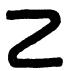
\includegraphics[keepaspectratio]{images/part002_ad0e6982551a0008e23df60b46a8b3d8f866f5ecbe9521df85283d9b8fea8d5c.jpg}}

The reader should beware of assuming that \(a + m = b + m\) implies a = b for all cardinals m (cf.~§6); * we shall see later, however, that this implication is true if m is finite (§5, no. 2, Proposition 3, Corollary 4 and §6, no. 3, Theorem 3, Corollary 4). *

\subsection{EXPONENTIATION OF CARDINALS}

DEFINITION 4. Let a and b be cardinals. The cardinal of the set of mappings of b into a is denoted by \(\mathfrak{a}^{\mathfrak{b}}\) , by abuse of notation.

The abuse of notation here lies in the fact that \(a^{b}\) already denotes the set of graphs of mappings of b into a (Chapter II, §5, no. 3), and this set is not necessarily a cardinal (Exercise 2). It will always be clear from the context which meaning is to be attached to the symbol \(a^{b}\) .

PROPOSITION 9. Let X and Y be two sets, a and b their respective cardinals. Then the set \(X^{Y}\) has cardinal \(a^{b}\) .

For there exists a bijection of \(\mathbf{X}^{\mathrm{Y}}\) onto the set of mappings of \(\mathfrak{b}\) into \(\mathfrak{a}\) (Chapter II, § 5, no. 2, Proposition 2, Corollary).

PROPOSITION 10. Let \(\mathfrak{a}\) and \(\mathfrak{b}\) be cardinals and let \(\mathbf{I}\) be a set such that Card (I) = \(\mathfrak{b}\) . If \(\mathfrak{a}_{\iota} = \mathfrak{a}\) for all \(\iota \in \mathbf{I}\) , we have \(\mathfrak{a}^{\mathfrak{b}} = \underset{\iota \in \mathbf{I}}{\mathsf{P}}\mathfrak{a}_{\iota}\) .

This follows from the definition of the product of a family of sets as a set of functional graphs (Chapter II, § 5, no. 3).

COROLLARY 1. Let \(\mathfrak{a}\) be a cardinal and let \((\mathfrak{b}_t)_{t\in I}\) be a family of cardinals. Then

\[
\mathfrak{a}^{\sum_{i \in I} \mathfrak{b}_i} = \underset {i \in I} {\mathbf {P}} \mathfrak{a}^{\mathfrak{b}_i}.
\]

Let S be the sum of the sets \(\mathfrak{b}_i\) , and put \(a_s = a\) for all \(s \in S\) . Both sides of the equality to be proved are then equal to \(\underset{s \in S}{\mathsf{P}} a_s\) , by virtue of Proposition 10 and the associativity formula for products (no. 3, Proposition 5(b)).

COROLLARY 2. Let \((\mathfrak{a}_i)_{i\in I}\) be a family of cardinals and let \(\mathfrak{b}\) be a cardinal. Then

\[
\left(\underset {i \in I} {\mathbf {P}} a _ {i}\right) ^ {b} = \underset {i \in I} {\mathbf {P}} a _ {i} ^ {b}.
\]

Let \(a_{i\beta} = a_i\) for each pair \((i, \beta) \in I \times b\) . Then, by associativity of the product, we have

\[
\left(\underset {i \in I} {\mathsf {P}} a _ {i}\right) ^ {\mathfrak {b}} = \underset {\beta \in \mathfrak {b}} {\mathsf {P}} \left(\underset {i \in I} {\mathsf {P}} a _ {i \beta}\right) = \underset {i \in I} {\mathsf {P}} \left(\underset {\beta \in \mathfrak {b}} {\mathsf {P}} a _ {i \beta}\right) = \underset {i \in I} {\mathsf {P}} a _ {i} ^ {\mathfrak {b}}.
\]

COROLLARY 3. Let \(a, b, c\) be cardinals. Then \(a^{bc} = (a^{b})^{c}\) .

Let \(\mathfrak{b}_{\gamma} = \mathfrak{b}\) for all \(\gamma \in \mathfrak{c}\) . Then

\[
a ^ {b c} = a ^ {\sum_ {\gamma \in c} b _ {\gamma}} = \underset {\gamma \in c} {\mathbf {P}} a ^ {b _ {\gamma}} = (a ^ {b}) ^ {c}
\]

by virtue of Corollary 1.

PROPOSITION 11. Let \(\mathfrak{a}\) be a cardinal. Then \(\mathfrak{a}^0 = 1\) , \(\mathfrak{a}^1 = \mathfrak{a}\) , \(1^{\mathfrak{a}} = 1\) ; and \(0^{\mathfrak{a}} = 0\) if \(\mathfrak{a} \neq 0\) .

For there exists a unique mapping of \(\varnothing\) into any given set (namely, the mapping whose graph is the empty set); the set of mappings of a set consisting of a single element into an arbitrary set X is equipotent to X (Chapter II, §5, no. 3); there exists a unique mapping of an arbitrary set into a set consisting of a single element; and, finally, there is no mapping of a non-empty set into \(\varnothing\) .

Note in particular that \(0^{0}=1\) .

PROPOSITION 12. Let X be a set and let a be its cardinal. Then the cardinal of the set \(\mathfrak{P}(X)\) of all subsets of \(X\) is \(2^{\mathfrak{a}}\) .

Let \(\alpha\) and \(\beta\) be the elements of the cardinal 2. For each subset Y of X let \(f_{\mathbf{Y}}\) be the mapping of X into 2 defined by \(f_{\mathbf{Y}}(x) = \alpha\) if \(x \in \mathbf{Y}\) and \(f_{\mathbf{Y}}(x) = \beta\) if \(x \in \mathbf{X} - \mathbf{Y}\) . Let \(u\) be the mapping \(\mathbf{Y} \to f_{\mathbf{Y}}\) of \(\mathfrak{P}(\mathbf{X})\) into \(2^{\mathbf{x}}\) . Conversely, with each mapping \(g\) of X into 2 let us associate the subset \(-g^{1}(\alpha)\) of X, and let \(v\) be the mapping \(g \to -g^{1}(\alpha)\) of \(2^{\mathbf{x}}\) into \(\mathfrak{P}(\mathbf{X})\) . It is clear that \(u \circ v\) and \(v \circ u\) are the identity mappings of \(2^{\mathbf{x}}\) and \(\mathfrak{P}(\mathbf{X})\) ; hence \(u\) and \(v\) are bijections (Chapter II, §3, no. 8, Proposition 8, Corollary) and therefore Card \((\mathfrak{P}(\mathbf{X})) = 2^{\mathbf{a}}\) .

\subsection{ORDER RELATION AND OPERATIONS ON CARDINALS}

PROPOSITION 13. Let \(\mathfrak{a}\) and \(\mathfrak{b}\) be cardinals. Then \(\mathfrak{a} \geqslant \mathfrak{b}\) if and only if there exists a cardinal \(\mathfrak{c}\) such that \(\mathfrak{a} = \mathfrak{b} + \mathfrak{c}\) .

For the relation \(a \geqslant b\) means that there exists a subset B of a which is equipotent to b (no. 2), i.e., a is equipotent to the set which is the sum of b and a set c.

\pandocbounded{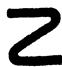
\includegraphics[keepaspectratio]{images/part002_f1d2aad8dae595af04a38c0526d2ebc1f30c28017ae785c1fe861e266dceeae2.jpg}}

If \(a \geqslant b\) , there usually exist many cardinals \(c\) such that \(a = b + c\) (cf.~§ 6); in general, therefore, it is not possible to define the ``difference'' \(a - b\) of two such cardinals (cf.~§ 5, no. 2).

PROPOSITION 14. Let \((\mathfrak{a}_i)_{i\in I}\) and \((\mathfrak{b}_i)_{i\in I}\) be two families of cardinals, both indexed by the same set \(I\) , and such that \(\mathfrak{a}_i\geqslant \mathfrak{b}_i\) for all \(i\in I\) . Then

\[
\sum_ {i \in I} a _ {i} \geqslant \sum_ {i \in I} b _ {i}, \quad \mathbf {P} _ {i \in I} a _ {i} \geqslant \mathbf {P} _ {i \in I} b _ {i}.
\]

The second inequality follows from the inclusion relations between products of sets (Chapter II, § 5, no. 4, Proposition 6, Corollary 3). As to the first inequality, if a set E is the union of a family \((\mathbf{A}_{t})_{t\in\mathbf{I}}\) of mutually disjoint subsets and if \(B_{t}\subset A_{t}\) for all \(t\in I\) , then the \(B_{t}\) are also mutually disjoint and \(\bigcup_{i}B_{i}\subset\bigcup_{i}A_{i}\) (Chapter II, § 4, no. 2).

COROLLARY 1. Let \((\mathfrak{a}_i)_{t \in I}\) be a family of cardinals. For each subset \(J\) of \(I\) we have \(\sum_{i \in J} \mathfrak{a}_i \leqslant \sum_{i \in I} \mathfrak{a}_i\) . If also \(\mathfrak{a}_i \neq 0\) for all \(i \in I - J\) , then \(\mathsf{P}_{i \in J} \mathfrak{a}_i \leqslant \mathsf{P}_{i \in I} \mathfrak{a}_i\) . Put \(\mathfrak{b}_i = \mathfrak{a}_i\) if \(i \in J\) , and \(\mathfrak{b}_i = 0\) (resp. \(\mathfrak{b}_i = 1\) ) if \(i \in I - J\) . Then apply Proposition 14, observing that the relation \(\mathfrak{a} \neq 0\) implies \(\mathfrak{a} \geqslant 1\) .

COROLLARY 2. If \(\mathfrak{a}\) , \(\mathfrak{a}'\) , \(\mathfrak{b}\) , \(\mathfrak{b}'\) are cardinals such that \(\mathfrak{a} \leqslant \mathfrak{a}'\) , \(\mathfrak{b} \leqslant \mathfrak{b}'\) , and \(\mathfrak{a}' > 0\) , then \(\mathfrak{a}^{\mathfrak{b}} \leqslant {\mathfrak{a}'}^{\mathfrak{b}'}\) .

For \(a^b \leqslant a'^b\) by Propositions 10 and 14, and \(a'^b \leqslant a'^{b'}\) by Proposition 10 and Corollary 1 to Proposition 14.

THEOREM 2 (Cantor). For each cardinal a, we have \(2^{\mathfrak{a}} > \mathfrak{a}\) .

We have \(\operatorname{Card}(\mathfrak{P}(\mathfrak{a})) = 2^{\mathfrak{a}}\) (no. 5, Proposition 12). The mapping \(x \to \{x\} (x \in \mathfrak{a})\) is an injection of \(\mathfrak{a}\) into \(\mathfrak{P}(\mathfrak{a})\) , whence \(\mathfrak{a} \leqslant 2^{\mathfrak{a}}\) . Hence it is enough to show that \(\mathfrak{a} \neq 2^{\mathfrak{a}}\) , i.e., that for every mapping \(f\) of \(\mathfrak{a}\) into \(\mathfrak{P}(\mathfrak{a})\) , the image \(f(\mathfrak{a})\) is distinct from \(\mathfrak{P}(\mathfrak{a})\) . Let \(\mathbf{X}\) be the set of all \(x \in \mathfrak{a}\) such that \(x \notin f(x)\) . If \(x \in \mathbf{X}\) , we have \(x \notin f(x)\) , whence \(f(x) \neq \mathbf{X}\) ; if \(x \in \mathfrak{a} - \mathbf{X}\) , we have \(x \in f(x)\) and \(x \notin \mathbf{X}\) , whence \(f(x) \neq \mathbf{X}\) . This shows that \(\mathbf{X} \notin f(\mathfrak{a})\) and proves the theorem.

COROLLARY. There does not exist a set that has every cardinal as an element.

If U were such a set, there would exist a set S, the sum of the family of sets \((\mathbf{X})_{\mathbf{x}\in\mathbf{U}}\) , so that every cardinal is equipotent to a subset of S. In particular, let \(\mathfrak{S}=\operatorname{Card}(\mathbf{S})\) ; since \(2^{S}\) is a cardinal, we would have \(2^{S}\leqslant S\) , in contradiction to Theorem 2.

\section{NATURAL INTEGERS. FINITE SETS}

\subsection{DEFINITION OF INTEGERS}

DEFINITION 1. A cardinal \(\mathfrak{a}\) is said to be finite if \(\mathfrak{a} \neq \mathfrak{a} + 1\) . A finite cardinal is also called a natural integer (or simply an integer if there is no risk of confusion (*)). A set \(\mathbf{E}\) is said to be finite if Card (E) is a finite cardinal; and Card (E) is then called the number of elements of \(\mathbf{E}\) .

A family (Chapter II, § 3, no. 4) is said to be finite if its index set is finite.

When we say that the number of objects of a certain type is an integer m, we mean that these objects are elements of a finite set whose number of elements is m. A set whose number of elements is m is also called a set of m elements.

PROPOSITION 1. A cardinal a is finite if and only if a + 1 is finite.

For the relations \(\mathfrak{a} = \mathfrak{b}\) and \(\mathfrak{a} + 1 = \mathfrak{b} + 1\) between cardinals \(\mathfrak{a}\) and \(\mathfrak{b}\) are equivalent (§ 3, no. 4, Proposition 8); the relations \(\mathfrak{a} \neq \mathfrak{a} + 1\) and \(\mathfrak{a} + 1 \neq (\mathfrak{a} + 1) + 1\) are therefore equivalent.

It is clear that \(0 \neq 1\) ; hence 0 is an integer. It follows that 1 and 2 are integers. The cardinals \(2 + 1\) and \((2 + 1) + 1\) are integers, denoted by 3 and 4, respectively.

\subsection{INEQUALITIES BETWEEN INTEGERS}

PROPOSITION 2. Let \(n\) be an integer. Then every cardinal \(\mathfrak{a}\) such that \(\mathfrak{a} \leqslant n\) is an integer. If \(n \neq 0\) , there exists a unique integer \(m\) such that \(n = m + 1\) , and the relation \(a < n\) is equivalent to \(a \leqslant m\) .

If \(\mathfrak{a} \leqslant n\) , there exists a cardinal \(\mathfrak{b}\) such that \(n = \mathfrak{a} + \mathfrak{b}\) (§ 3, no. 6, Proposition 13). Then \((\mathfrak{a} + 1) + \mathfrak{b} = (\mathfrak{a} + \mathfrak{b}) + 1 = n + 1\) (§ 3, no. 3, Proposition 5, Corollary); and since \(n \neq n + 1\) , we have

\[
(a + 1) + b \neq a + b.
\]

Hence \(\mathfrak{a} + 1 \neq \mathfrak{a}\) , which means that \(\mathfrak{a}\) is an integer. If \(n \neq 0\) , we have \(n \geqslant 1\) (§3, no. 2), and therefore there exists a unique cardinal \(m\) such that \(n = m + 1\) (§3, no. 6, Proposition 13 and no. 4, Proposition 8). Since \(m \leqslant n\) , \(m\) is an integer, from what has already been proved. Finally, if an integer \(a\) is such that \(a < n\) , we have \(n = a + b\) , with \(b \neq 0\) (§3, no. 6, Proposition 13); since \(b\) is an integer, we have \(b = c + 1\) and \(n = m + 1 = (a + c) + 1\) . It follows that \(m = a + c\) (§3, no. 4, Proposition 8), hence \(a \leqslant m\) . Conversely, if \(a \leqslant m\) , we have

\[
a \leqslant m + 1 = n;
\]

and if \(a = n = m + 1\) , we would have \(a > m\) , contrary to hypothesis.

COROLLARY 1. Every subset of a finite set is finite.

COROLLARY 2. If X is a subset of a finite set E and X ≠ E, then

\[
\text { Card } (\mathbf {X}) <   \text { Card } (\mathbf {E}).
\]

For X is contained in the complement \(X'\) of a subset of E consisting of a single element; we have \(\text{Card}(X) \leqslant \text{Card}(X')\) and \(\text{Card}(E) = \text{Card}(X') + 1\) , hence (Proposition 2) \(\text{Card}(X') < \text{Card}(E)\) and a fortiori \(\text{Card}(X) < \text{Card}(E)\) .

Definition 1 shows that, conversely, if E is a set such that

\[
\operatorname{Card} (\mathbf {X}) <   \operatorname{Card} (\mathbf {E})
\]

for every subset X of E such that \(X \neq E\) , then E is finite.

COROLLARY 3. If \(f\) is a mapping of a finite set \(\mathbf{E}\) into a set \(\mathbf{F}\) , then \(f(\mathbf{E})\) is a finite subset of \(\mathbf{F}\) .

For Card \((f(\mathbf{E}))\leqslant\) Card (E) (§ 3, no. 2, Proposition 3).

COROLLARY 4. Let E and F be two finite sets with the same number of elements, and let f be a mapping of E into F. Then the following statements are equivalent :

\begin{enumerate}
\def\labelenumi{(\alph{enumi})}
\item
  \(f\) is an injection;
\item
  \(f\) is a surjection;
\item
  \(f\) is a bijection.
\end{enumerate}

It is enough to prove that (a) and (b) are equivalent. If \(f\) is injective, then \(\operatorname{Card}(f(\mathbf{E})) = \operatorname{Card}(\mathbf{E}) = \operatorname{Card}(\mathbf{F})\) , whence \(f(\mathbf{E}) = \mathbf{F}\) (Corollary 2). If \(f\) is not injective, let \(x\) and \(x'\) be two elements of \(\mathbf{E}\) such that \(x \neq x'\) and \(f(x) = f(x')\) . Then, putting \(\mathbf{E}' = \mathbf{E} - \{x\}\) , we have \(f(\mathbf{E}') = f(\mathbf{E})\) , whence \(\operatorname{Card}(f(\mathbf{E})) \leqslant \operatorname{Card}(\mathbf{E}') < \operatorname{Card}(\mathbf{E})\) by virtue of Corollary 2; but since \(\operatorname{Card}(\mathbf{F}) = \operatorname{Card}(\mathbf{E})\) , it follows that \(f(\mathbf{E}) \neq \mathbf{F}\) .

\subsection{THE PRINCIPLE OF INDUCTION}

C61 (Principle of Induction). Let \(\mathbb{R}\{n\}\) be a relation in a theory \(\mathfrak{C}\) (where \(n\) is not a constant of \(\mathfrak{C}\) ). Suppose that the relation

\[
\mathrm{R} \{0 \} \text { and } (\forall n) ((n \text { is   an   integer   and } \mathrm{R} \{n \}) \Longrightarrow \mathrm{R} \{n + 1 \})
\]

is a theorem in \(\mathfrak{C}\) . Under these conditions the relation

\[
(\forall n) ((n \text {   is   an   integer   }) \Longrightarrow R \{n \})
\]

is a theorem in \(\mathfrak{C}\) .

We shall argue by contradiction. Suppose that the relation

\[
(\exists n) (n \text {   is   an   integer   and   } (\text { not   } R \{n \}))
\]

is true. Let \(q\) be an integer such that ``not \(\mathbb{R}\{q\}\) '' (method of the auxiliary constant; cf.~Chapter I, §3, no. 3 and §4, no. 1). The integers \(n\) for which `` \(n \leqslant q\) and (not \(\mathbb{R}\{n\}\) )'' form a well-ordered non-empty set (§3, no. 2, Remark), which therefore has a least element \(s\) . If \(s = 0\) , then ``not \(\mathbb{R}\{0\}\) '', contrary to hypothesis. If \(s > 0\) , then \(s = s' + 1\) , where \(s'\) is an integer such that \(s' < s\) (no. 2, Proposition 2). By definition of \(s\) , we have \(\mathbb{R}\{s'\}\) , but then the hypothesis implies that \(\mathbb{R}\{s\}\) is true, contrary to the definition of \(s\) .

In order to apply the principle of induction it is necessary in particular to prove the relation

\[
(n \text {   is   an   integer   and   } R \{n \}) \Longrightarrow R \{n + 1 \}.
\]

For this purpose the method of the auxiliary hypothesis (Chapter I, §3, no. 3) is commonly used, and it is for this reason that the relation ``n is an integer and R\{n\}'' (or even R\{n\}) is called the inductive hypothesis.

Remark. There are various criteria which are frequently used under the name of ``principle of induction''. They can all be easily deduced from C61, and we indicate here the most important of them:

\begin{enumerate}
\def\labelenumi{(\arabic{enumi})}
\tightlist
\item
  Let \(\mathbf{S}\{n\}\) be the relation
\end{enumerate}

\((\forall p)((n \text{ is an integer and } p \text{ is an integer and } p < n) \Longrightarrow \mathbb{R}\{p\})\)

and suppose that \(S\{n\}\) implies \(R\{n\}\) . Then the relation

\[
(\forall n) ((n \text {   is   an   integer   }) \Longrightarrow R \{n \})
\]

is true. For the relation \(S\{0\}\) is true, and by hypothesis \(S\{n\}\) implies \(R\{n\}\) ; since the relation \(m < n + 1\) is equivalent to \(m \leqslant n\) (no. 2, Proposition 2), the relation \(S\{n + 1\}\) is equivalent to `` \(S\{n\}\) and \(R\{n\}\) '', consequently, \(S\{n\}\) implies \(S\{n + 1\}\) . The criterion C61 therefore proves that the relation

\[
(\forall n) ((n \text {   is   an   integer   }) \Longrightarrow \mathrm{S} \{n \})
\]

is true, and since \(\mathbf{S}\{n\}\) implies \(\mathbf{R}\{n\}\) , the relation

\[
(\forall n) ((n \text {   is   an   integer   }) \Longrightarrow R \{n \})
\]

is true.

\begin{enumerate}
\def\labelenumi{(\arabic{enumi})}
\setcounter{enumi}{1}
\tightlist
\item
  Let \(k\) be an integer and let \(\mathbf{R}\{n\}\) be a relation such that the relation
\end{enumerate}

\[
\mathrm{R} \{k \} \text { and } (\forall n) ((n \text { is   an   integer } \geqslant k \text { and } \mathrm{R} \{n \}) \Longrightarrow \mathrm{R} \{n + 1 \})
\]

is true. Then the relation

\[
(\forall n) ((n \text {   is   an   integer   } \geqslant k) \Longrightarrow \mathrm{R} \{n \})
\]

is true (``induction starting at \(k\)''). For let \(S\{n\}\) be the relation

\[
(n \geqslant k) \Longrightarrow \mathrm{R} \{n \}.
\]

Then by the method of disjunction of cases we see that S\{0\} is true. On the other hand, it is easily verified that the relation

\[
(n \text {   is   an   integer   and   } S \{n \}) \Longrightarrow S \{n + 1 \}
\]

is true. It follows from C61 that the relation

\[
(n \text {   is   an   integer) } \implies \mathrm{S} \{n \}
\]

is true, which proves our assertion.

\begin{enumerate}
\def\labelenumi{(\arabic{enumi})}
\setcounter{enumi}{2}
\tightlist
\item
  Let \(a\) and \(b\) be two integers such that \(a \leqslant b\) , and let \(R\{n\}\) be a relation such that
\end{enumerate}

\[
\mathrm{R} \left\{a \right\} \text {   and   } (\forall n) ((n \text {   is   an   integer   and   } a \leqslant n <   b \text {   and   } \mathrm{R} \left\{n \right\}) \Longrightarrow \mathrm{R} \left\{n + 1 \right\}).
\]

Then the relation

\[
(\forall n) ((n \text {   is   an   integer   and   } a \leqslant n \leqslant b) \Longrightarrow \mathrm{R} \{n \})
\]

is true. The proof is similar to that of the preceding case; we take S\{n\} to be the relation ``(a ≤ n \textless{} b) ⇒ R\{n\}'' (``induction restricted to an interval'').

\begin{enumerate}
\def\labelenumi{(\arabic{enumi})}
\setcounter{enumi}{3}
\tightlist
\item
  Let \(a, b\) be two integers such that \(a \leqslant b\) , and let \(\mathbf{R}\{n\}\) be a relation such that
\end{enumerate}

\(R\{b\}\) and \((\forall n)((n \text{ is an integer and } a \leqslant n < b \text{ and } R\{n + 1\}) \Longrightarrow R\{n\}).\)

Then the relation

\[
(\forall n) ((n \text {   is   an   integer   and   } a \leqslant n \leqslant b) \Longrightarrow \mathrm{R} \{n \})
\]

is true. For we have the relation

(n is an integer and \(a \leqslant n < b\) and (not \(\mathbf{R}\{n\}\) ) \(\Longrightarrow\) not \(\mathbf{R}\{n + 1\}\) .

If for some \(n\) such that \(a \leqslant n \leqslant b\) we had (not \(\mathbf{R}\{n\}\) ), it would follow from (3) that (not \(\mathbf{R}\{b\}\) ), contrary to the hypothesis, whence the result (``descending induction'').

\subsection{FINITE SUBSETS OF ORDERED SETS}

PROPOSITION 3. Let E be a right directed preordered set (resp. a lattice, resp. a totally ordered set). Then every non-empty finite subset of E is bounded above (resp. has a least upper bound and a greatest lower bound, resp. has a greatest element and a least element).

The proof is by induction on the number n of elements of the subset under consideration. The result is trivial for n = 1. Let X be a subset of \(n + 1\) elements of E (with \(n \geqslant 1\) ), and put \(X = Y \cup \{x\}\) , where Y has n elements and is therefore not empty. The inductive hypothesis implies the existence of an upper bound (resp. least upper bound, resp. greatest element) y of Y. Since E is right directed (resp. a lattice, resp. totally ordered), \(\{x, y\}\) has an upper bound (resp. least upper bound, resp. greatest element) which is evidently an upper bound (resp. least upper bound, resp. greatest element) of X.

COROLLARY 1. Every totally ordered finite set is well-ordered and has a greatest element.

COROLLARY 2. Every finite ordered set has a maximal element.

For such a set is inductive by Corollary 1 (cf.~§2, no. 4, Theorem 2).

\subsection{PROPERTIES OF FINITE CHARACTER}

DEFINITION 2. Let E be a set. A set S of subsets of E is said to be of finite character if the relation X ∈ S is equivalent to the relation ``every finite subset of X belongs to S''.

A property \(P\{X\}\) of a subset X of a set E is said to be of finite character if the set of subsets X of E for which \(P\{X\}\) is true is of finite character.

\minorheading{Examples}

\begin{enumerate}
\def\labelenumi{(\arabic{enumi})}
\tightlist
\item
  The set of totally ordered subsets of an ordered set E is of finite character. Indeed, a subset X of E is totally ordered if and only if every subset of X consisting of two elements is totally ordered.
\end{enumerate}

* (2) The set of all free subsets of a module is of finite character. The same is true of the set of all algebraically free subsets of an extension of a field.

\begin{enumerate}
\def\labelenumi{(\arabic{enumi})}
\setcounter{enumi}{2}
\tightlist
\item
  The set of submodules of a module E is not of finite character, because a finite subset of a submodule of E is not necessarily a submodule of E. *
\end{enumerate}

THEOREM 1. Every set S of subsets of a set E which is of finite character has a maximal element (when ordered by inclusion).

By Theorem 2 of §2, no. 4 it is enough to show that \(\mathfrak{S}\) is inductive. To do this we shall show that if \(\mathfrak{G}\) is any subset of \(\mathfrak{S}\) which is totally ordered by inclusion, the union X of the sets of \(\mathfrak{G}\) belongs to \(\mathfrak{S}\) (§2, no. 4, Theorem 2, Corollary 2). Since \(\mathfrak{S}\) is of finite character, it is enough to show that every finite subset Y of X belongs to \(\mathfrak{S}\) . Now, for each \(y \in Y\) , there exists a set \(Z_y \in \mathfrak{G}\) such that \(y \in Z_y\) . Since the set of sets \(Z_y\) ( \(y \in Y\) ) is finite and totally ordered by inclusion, it has a greatest element S (no. 4, Corollary 1 to Proposition 3); in other words, there exists a set \(S \in \mathfrak{G}\) such that \(Y \subset S\) . But since \(S \in \mathfrak{S}\) and since Y is a finite subset of S, we have \(Y \in \mathfrak{S}\) because \(\mathfrak{S}\) is of finite character; this completes the proof.

\section{PROPERTIES OF INTEGERS}

\subsection{OPERATIONS ON INTEGERS AND FINITE SETS}

PROPOSITION 1. Let \((a_i)_{i\in I}\) be a finite family of integers. Then the cardinals \(\sum_{i\in I}a_i\) and \(\prod_{i\in I}a_i\) are integers.

Let us begin by showing that if \(a\) and \(b\) are integers, then so is \(a + b\) . We proceed by induction on \(b\) . The assertion is true for \(b = 0\) since \(a + 0 = a\) . If \(a + b\) is an integer, then so is \((a + b) + 1\) ( \(\S 4\) , no. 1, Proposition 1). But \((a + b) + 1 = a + (b + 1)\) ( \(\S 3\) , no. 3, Corollary to Proposition 5); hence \(a + (b + 1)\) is an integer, and consequently \(a + b\) is an integer for all integers \(b\) .

Next we show by induction on \(n = \operatorname{Card}(\mathbf{I})\) that \(\sum_{i \in \mathbf{I}} a_i\) is an integer. This is clear if \(n = 0\) , for then \(\mathbf{I} = \emptyset\) and \(\sum_{i \in \mathbf{I}} a_i = 0\) . If \(\operatorname{Card}(\mathbf{I}) = n + 1\) , we may write \(\mathbf{I} = \mathbf{J} \cup \{k\}\) , where \(\operatorname{Card}(\mathbf{J}) = n\) and \(k \notin \mathbf{J}\) . Then

\[
\sum_ {i \in \mathbf {I}} a _ {i} = a _ {k} + \sum_ {i \in \mathbf {J}} a _ {i}
\]

(§ 3, no. 3, Proposition 5). The inductive hypothesis is that \(\sum_{i\in J}a_i\) is an integer; hence so is \(a_{k} + \sum_{i\in J}a_{i}\) , from the first paragraph of the proof. This shows that \(\sum_{i\in I}a_{i}\) is an integer for all \(n\) .

Since the product ab of two integers a and b is the sum of a finite family of integers all equal to a (§3, no. 4, Proposition 6, Corollary 2), ab is an integer. We shall prove by induction on n = Card (I) that \(\prod_{i\in I}a_{i}\) is an integer. This is true for n = 0, because then

\[
\prod_ {i \in \mathbf {I}} a _ {i} = 1.
\]

If Card (I) = n + 1, we have (with the same notation as above)

\[
\prod_ {i \in \mathbf {I}} a _ {i} = a _ {k}. \prod_ {i \in \mathbf {J}} a _ {i}
\]

(§ 3, no. 3, Proposition 5), and the inductive hypothesis therefore implies that \(\prod_{i\in I}a_i\) is an integer. Consequently \(\prod_{i\in I}a_i\) is an integer for all \(n\) .

COROLLARY 1. The union E of a finite family \((\mathbf{X}_i)_{i\in \mathbf{I}}\) of finite sets is a finite set.

For the sum S of the family \((\mathbf{X}_{i})\) is finite; and since there exists a mapping of S onto E (Chapter II, §4, no. 8), the set E is finite (§4, no. 2, Proposition 2, Corollary 3).

COROLLARY 2. The product of a finite family of finite sets is a finite set.

COROLLARY 3. If \(a\) and \(b\) are integers, \(a^b\) is an integer.

For \(a^b\) is the product of a finite family of integers all equal to \(a\) (§ 3, no. 5, Proposition 10).

COROLLARY 4. The set of subsets of a finite set E is finite.

For its cardinal is \(2^{\text{Card (E)}}\) ( \(\S 3\) , no. 5, Proposition 12).

\subsection{STRICT INEQUALITIES BETWEEN INTEGERS}

PROPOSITION 2. Let \(a\) and \(b\) be two integers. Then \(a < b\) if and only if there exists an integer \(c > 0\) such that \(b = a + c\) .

If \(a < b\) , there exists a cardinal \(c \leqslant b\) (so that \(c\) is an integer ( \(\S 4\) , no. 2, Proposition 2)) such that \(b = a + c\) ( \(\S 3\) , no. 6, Proposition 13); if \(a \neq b\) , we must have \(c \neq 0\) . Conversely, if \(b = a + c\) and \(c \neq 0\) , then \(c \geqslant 1\) and hence \(a < a + 1 \leqslant a + c = b\) .

PROPOSITION 3. Let \((a_i)_{i \in I}\) and \((b)_{i \in I}\) be two finite families of integers such that \(a_i \leqslant b_i\) for each \(i \in I\) and \(a_i < b_i\) for at least one index \(i\) . Then

\[
\sum_ {i \in \mathbf {I}} a _ {i} <   \sum_ {i \in \mathbf {I}} b _ {i}.
\]

If also \(b_{i} > 0\) for each \(i \in \mathbf{I}\) , then

\[
\prod_ {i \in I} a _ {i} <   \prod_ {i \in I} b _ {i}.
\]

Let \(j\) be an index such that \(a_{j} < b_{j}\) , and let \(J = I - \{j\}\) . Then

\[
b _ {j} = a _ {j} + c _ {j}
\]

with \(c_{j} > 0\) (Proposition 2), and therefore (§ 3, no. 6, Proposition 14)

\[
\sum_ {i \in \mathbf {I}} b _ {i} = a _ {j} + c _ {j} + \sum_ {i \in \mathbf {J}} b _ {i} \geqslant c _ {j} + a _ {j} + \sum_ {i \in \mathbf {J}} a _ {i} = c _ {j} + \sum_ {i \in \mathbf {I}} a _ {i}.
\]

Since \(c_{j} > 0\) , the first part of the Proposition follows from Proposition 2. Likewise

\[
\prod_ {i \in I} b _ {i} = (a _ {j} + c _ {j}) \prod_ {i \in J} b _ {i} = a _ {j}. \prod_ {i \in J} b _ {i} + c _ {j}. \prod_ {i \in J} b _ {i} \geqslant \prod_ {i \in I} a _ {i} + c _ {j}. \prod_ {i \in J} b _ {i}.
\]

Since \(c_{j}\) and all the \(b_{i}\) are \(\neq 0\) , the product \(c_{j}\) . \(\prod_{i \in \mathbb{J}} b_{i}\) is \(\neq 0\) (§3, no. 4, Proposition 7); hence the second part of the Proposition.

COROLLARY 1. Let \(a, a',\) and \(b\) be integers such that \(a < a'\) and \(b > 0\) . Then \(a^b < a'^b\) .

We need only express \(a^b\) and \(a'^b\) as products of finite families of integers (§ 3, no. 5, Proposition 10) and apply Proposition 3, observing that the relation \(a < a'\) implies \(a' > 0\) .

COROLLARY 2. Let \(a, b\) , and \(b'\) be integers such that \(a > 1\) and \(b < b'\) ; then \(a^b < a^{b'}\) .

For there exists an integer \(c > 0\) such that \(b' = b + c\) (Proposition 2); since \(c \geqslant 1\) , we have \(a^c \geqslant a > 1\) , whence \(a^{b'} = a^b a^c > a^b\) .

COROLLARY 3. Let \(a, b, b'\) be integers (resp. integers such that \(a > 0\) ). Then \(a + b = a + b'\) (resp. \(ab = ab'\) ) if and only if \(b = b'\) .

COROLLARY 4. If \(a\) and \(b\) are integers such that \(a \leqslant b\) , then there exists a unique integer \(c\) such that \(b = a + c\) .

The existence of \(c\) follows from Proposition 13 of §3, no. 6, and its uniqueness from Corollary 3 above.

The integer \(c\) such that \(b = a + c\) (where \(a \leqslant b\) ) is called the difference of the integers \(b\) and \(a\) , and is written \(b - a\) . It is easily verified that if \(a, b, a', b'\) are integers such that \(a \leqslant b\) and \(a' \leqslant b'\) , then

\[
(b - a) + (b ^ {\prime} - a ^ {\prime}) = (b + b ^ {\prime}) - (a + a ^ {\prime}).
\]

\subsection{INTERVALS IN SETS OF INTEGERS}

Every set of integers, being a set of cardinals, is well-ordered (§ 3, no. 2, Theorem 1). Furthermore, for each integer \(a\) the relation `` \(x\) is a cardinal and \(x \leqslant a\) '' is collectivizing in \(x\) (§ 3, no. 2, Remark after Theorem 1), and the set of \(x\) which satisfy this relation is a set of integers (§ 4, no. 2, Proposition 2), which may therefore be denoted by {[}0, a{]}.

PROPOSITION 4. Let \(a\) and \(b\) be integers. Then the mapping \(x \to a + x\) is a strictly increasing isomorphism of the interval \([0, b]\) onto the interval \([a, a + b]\) , and \(y \to y - a\) is the inverse isomorphism.

Clearly the relations \(0 \leqslant x \leqslant b\) imply \(a \leqslant a + x \leqslant a + b\) . The mapping \(x \to a + x\) is strictly increasing (and therefore injective) by Proposition 3 of no. 2. Finally, the relations \(a \leqslant y \leqslant a + b\) imply \(y = a + x\) with \(x \geqslant 0\) and \(a + x \leqslant a + b\) , whence \(x \leqslant b\) (no. 2, Proposition 3). This completes the proof.

PROPOSITION 5. If \(a\) and \(b\) are integers such that \(a \leqslant b\) , then the interval \([a, b]\) is a finite set whose number of elements is \(b - a + 1\) .

By Proposition 4 we may restrict ourselves to the case where \(a=0\) . The proof is by induction on \(b\) . If \(b=0\) , the result is clear. The relation \(0 \leqslant x \leqslant b+1\) is equivalent to `` \(0 \leqslant x < b+1\) or \(x=b+1\) '', and the relation \(0 \leqslant x < b+1\) is equivalent to \(0 \leqslant x \leqslant b\) (§ 4, no. 2, Proposition 2); in other words, the interval \([0, b+1]\) is the union of \([0, b]\) and \(\{b+1\}\) , and these two sets are disjoint. By the inductive hypothesis the number of elements of \([0, b+1]\) is equal to \((b+1)+1\) , and the Proposition is proved.

PROPOSITION 6. For every finite set \(\mathbf{E}\) which is totally ordered and has \(n\) elements \((n \geqslant 1)\) , there exists a unique isomorphism of \(\mathbf{E}\) onto the interval \([1, n]\) .

Since E and \([1, n]\) are well-ordered (§4, no. 4, Proposition 3, Corollary 1) and have the same number of elements (Proposition 5), the result follows from Theorem 3 of §2, no. 5 and Corollary 2 to Proposition 2 of §4, no. 2.

\subsection{FINITE SEQUENCES}

A finite sequence (resp. finite sequence of elements of a set E) is a family (resp. a family of elements of E) whose index set I is a finite set of integers. The number of elements of I is called the length of the sequence.

Let \((t_i)_{i \in I}\) be a finite sequence of length \(n\) . By Proposition 6 of no. 3 there exists a unique isomorphism \(f\) of the interval \([1, n]\) onto the set of integers \(I\) . For each \(k \in [1, n]\) , \(t_{f(k)}\) is said to be the \(k\) th term of the sequence; \(t_{f(1)}\) (resp. \(t_{f(n)}\) ) is the first (resp. last) term of the sequence.

Let \(P\{i\}\) be a relation such that the elements \(i\) for which \(P\{i\}\) is true form a finite set of integers. A finite sequence \((t_i)_{i \in I}\) is then often written \((t_i)_{P\{i\}}\) . For example, when \(I = [a, b]\) , the notation \((t_i)_{a \leqslant i \leqslant b}\) is often used. Under the same conditions, to denote the product of a family of sets \((X_i)_{i \in I}\) the notations

\[
\prod_ {\mathrm{P} \{i \}} \mathrm{X} _ {i} \quad \text { and } \quad \prod_ {i = a} ^ {b} \mathrm{X} _ {i}
\]

are used; and analogous notations for union, intersection, cardinal product, cardinal sum, * composition laws in Algebra *, and so on.

\subsection{CHARACTERISTIC FUNCTIONS OF SETS}

Let E be a non-empty set and A a subset of E. The characteristic function of the subset A of E is the mapping \(\varphi_{A}\) of E into the set \(\{0, 1\}\) defined by

\[
\varphi_ {\mathbf {A}} (x) = 1 \quad \text { if } \quad x \in \mathbf {A}; \qquad \varphi_ {\mathbf {A}} (x) = 0 \quad \text { if } \quad x \in \mathbf {E} - \mathbf {A}.
\]

Clearly the relation \(\varphi_{\mathbf{A}} = \varphi_{\mathbf{B}}\) is equivalent to \(\mathbf{A} = \mathbf{B}\) . We have \(\varphi_{\mathbf{E}}(x) = 1\) for all \(x \in \mathbf{E}\) and \(\varphi_{\emptyset}(x) = 0\) for all \(x \in \mathbf{E}\) ; these are the only constant characteristic functions on \(\mathbf{E}\) . The following Proposition is an immediate consequence of the definitions:

PROPOSITION 7. For each pair of subsets A, B of a non-empty set E, we have

\begin{enumerate}
\def\labelenumi{(\arabic{enumi})}
\tightlist
\item
\end{enumerate}

\[
\varphi_ {\mathbf {E} - \mathbf {A}} (x) = 1 - \varphi_ {\mathbf {A}} (x),\tag{2}
\]

\[
\varphi_ {\mathbf {A} \cap \mathbf {B}} (x) = \varphi_ {\mathbf {A}} (x) \varphi_ {\mathbf {B}} (x),\tag{3}
\]

\[
\varphi_ {\mathbf {A} \cup \mathbf {B}} (x) + \varphi_ {\mathbf {A} \cap \mathbf {B}} (x) = \varphi_ {\mathbf {A}} (x) + \varphi_ {\mathbf {B}} (x)
\]

for all \(x \in E\) .

\subsection{EUCLIDEAN DIVISION}

THEOREM 1. Let \(a\) and \(b\) be integers such that \(b > 0\) . Then there exist integers \(q\) and \(r\) such that \(a = bq + r\) and \(r < b\) , and the integers \(q\) and \(r\) are uniquely determined by these conditions.

The conditions on \(q\) and \(r\) are equivalent to \(bq \leqslant a < b(q + 1)\) and \(r = a - bq\) (no. 2, Proposition 2). Hence we have to find \(q\) such that \(bq \leqslant a < b(q + 1)\) ; in other words, \(q\) must be the smallest integer such that \(a < b(q + 1)\) , which shows that \(q\) and \(r = a - bq\) are uniquely determined. To prove their existence, we note that there exist integers \(p\) such that \(a < bp\) , for example \(a + 1\) (since \(b > 0\) ). Let \(m\) be the least of these integers. We have \(m \neq 0\) , and we may therefore write \(m = q + 1\) with \(q \leqslant m\) ( \(\S 4\) , no. 2, Proposition 2); it follows that \(bq \leqslant a < b(q + 1)\) .

DEFINITION 1. With the notation of Theorem 1, r is called the remainder of the division of a by b. If r = 0, we say that a is a multiple of b, or that a is divisible by b, or that b is a divisor of a, or that b divides a, or that b is a factor of a. The number q is then called the quotient of a by b and is denoted by \(\frac{a}{b}\) or a/b.

If \(a\) is not a multiple of \(b\) , the number \(q\) is called the integral part of the quotient of \(a\) by \(b\) (cf.~General Topology, Chapter IV, §8, no. 2).

In this chapter, writing \(a / b\) or \(\frac{a}{b}\) will imply that \(b\) divides \(a\) .

The relations \(a = bq\) and \(q = a / b\) are equivalent (if \(b > 0\) ). Every multiple \(a'\) of a multiple \(a\) of \(b\) is a multiple of \(b\) , and

\[
a ^ {\prime} / b = (a ^ {\prime} / a) (a / b) \quad \text { if } \quad a \neq 0.
\]

Also, if \(c\) and \(d\) are multiples of \(b\) , then \(c + d\) and \(c - d\) (if \(d \leqslant c\) ) are multiples of \(b\) , and we have

\[
\frac {c + d}{b} = \frac {c}{b} + \frac {d}{b}, \quad \frac {c - d}{b} = \frac {c}{b} - \frac {d}{b}.
\]

The integers which are multiples of 2 are said to be even, and the others odd. By Theorem 1 the odd integers are of the form \(2n + 1\) .

\subsection{EXPANSION TO BASE b}

PROPOSITION 8. Let \(b\) be an integer \(> 1\) . For each integer \(k > 0\) let \(\mathbf{E}_k\) be the lexicographic product (§2, no. 6) of the family \((\mathrm{J}_h)_{0 \leqslant h \leqslant k-1}\) of intervals all identical with {[}0, \(b - 1\) {]}. For each \(r = (r_0, r_1, \ldots, r_{k-1}) \in \mathbf{E}_k\) , let \(f_k(r) = \sum_{h=0}^{k-1} r_h b^{k-h-1}\) ; then the mapping \(f_k\) is an isomorphism of the ordered set \(\mathbf{E}_k\) onto the interval {[}0, \(b^k - 1\) {]}.

The proof is by induction on \(k\) . For \(k = 1\) it is an immediate consequence of the definitions. For each \(r = (r_0, \ldots, r_{k-1}, r_k) \in \mathbf{E}_{k+1}\) , put

\[
\varphi (r) = \left(r _ {0}, \dots , r _ {k - 1}\right) \in \mathrm{E} _ {k}.
\]

Then the mapping \(r \to (\varphi(r), r_k)\) is an isomorphism of \(\mathbf{E}_{k+1}\) onto the lexicographical product of \(\mathbf{E}_k\) and \(J = [0, b - 1]\) ; this is immediate from the definitions. We may write

\[
f _ {k + 1} (r) = b \cdot f _ {k} (\varphi (r)) + r _ {k};
\]

let us show that the relation \(r < r'\) in \(\mathbf{E}_{k+1}\) implies \(f_{k+1}(r) < f_{k+1}(r')\) . Indeed, we have either \(\varphi(r) < \varphi(r')\) , or else \(\varphi(r) = \varphi(r')\) and \(r_k < r'_k\) . In the first case, the inductive hypothesis implies that \(f_k(\varphi(r)) < f_k(\varphi(r'))\) , and therefore (§4, no. 2, Proposition 2) \(f_k(q(r')) \geqslant f_k(\varphi(r)) + 1\) ; consequently

\[
f _ {k - 1} (r ^ {\prime}) \geqslant b. f _ {k} (\varphi (r)) + b > f _ {k + 1} (r),
\]

since \(r_k \leqslant b - 1\) (no. 2, Proposition 3). If, on the other hand, \(\varphi(r) = \varphi(r')\) and \(r_k < r_k'\) , it is clear that \(f_{k+1}(r) < f_{k+1}(r')\) . Now the inductive hypothesis shows that \(f_k(\varphi(r)) \leqslant b^k - 1\) , whence

\[
f _ {k + 1} (r) \leqslant b (b ^ {k} - 1) + b - 1 = b ^ {k + 1} - 1.
\]

It follows that \(f_{k+1}\) is an isomorphism of \(\mathbf{E}_{k+1}\) onto a subset of the interval \([0, b^{k+1} - 1]\) ; but this interval and \(\mathbf{E}_{k+1}\) have the same number of elements, namely \(b^{k+1}\) (no. 3, Proposition 5); therefore \(f_{k+1}\) is a bijection (§4, no. 2, Proposition 2, Corollary 4), and the proof is complete.

¶ We note now that for every integer \(a\) we have \(a < b^a\) . This is proved by induction on \(a\) ; the result is evident for \(a = 0\) , and the hypothesis \(a < b^a\) implies \(a + 1 \leqslant b^a < b \cdot b^a = b^{a+1}\) (no. 2, Proposition 3 and §4, no. 2, Proposition 2). There is therefore a least integer \(k\) such that \(a < b^k\) , and Proposition 8 then shows that there exists a unique finite sequence \((r_h)_{0 \leqslant h \leqslant k-1}\) such that \(0 \leqslant r_h \leqslant b - 1\) for \(0 \leqslant h \leqslant k - 1\) and

\[
a = \sum_ {h = 0} ^ {k - 1} r _ {h} b ^ {k - h - 1}.
\]

Furthermore, we must have \(r_{0} > 0\) , for otherwise \(a < b^{k-1}\) by virtue of Proposition 8. The expression

\[
\sum_ {h = 0} ^ {k - 1} r _ {h} b ^ {k - h - 1}
\]

is called the expansion to base b of the integer a.

* In all parts of mathematics which do not involve numerical computations, Proposition 8 is useful mainly when applied to a prime number \(b\) . *

When the integer b is small enough for this to be practicable, we may represent each integer \textless b by a distinctive symbol called a digit. The digits which represent 0 and 1 are usually 0 and 1. Let a be an integer \(_{k-1}\)

and let \(\sum_{h=0}^{r_h b^{k-h-1}}\) be its expansion to base \(b\) . If the integer \(k\) which

appears in this expansion is sufficiently small for this to be practicable, it is usual to associate with the integer \(a\) the succession of symbols obtained by writing \(r_0r_1 \ldots r_{k-2}r_{k-1}\) from left to right and then replacing each integer \(r_i\) by the digit which represents it; the symbol so obtained is called the numerical symbol associated with \(a\) . One then often replaces \(a\) by its numerical symbol in the terms and relations in which it appears.

For example, if C, Q, F, D are digits, the numerical symbols CQ, CQF, CQFD are respectively associated with \(Cb + Q\) , \(Cb^{2} + Qb + F\) , \(Cb^{2} + Qb^{2} + Fb + D\) .

It follows from Proposition 8 that the numerical symbol associated with an integer a is unique, and that if \(a < b^{k}\) it contains at most k digits. Notice that the numerical symbol associated with the integer \(b^{k}\) consists of the digit 1 followed by k digits 0.

This system of representation of integers by numerical symbols is called the system of numeration to base b. In practical numerical computations, the following systems are used: (a) the system to base 2, or the dyadic system, in which the digits are 0 and 1; (b) the decimal system, in which the digits are 0, 1, 2, 3, 4, \(5 = 4 + 1\) , \(6 = 5 + 1\) , \(7 = 6 + 1\) , \(8 = 7 + 1\) , \(9 = 8 + 1\) , and in which \(b\) is the integer \(9 + 1\) (whose numerical symbol in this system is therefore 10).

Since the Middle Ages the decimal system has been traditionally used in numerical calculations, and we shall use it in this series whenever we have occasion to write down an integer explicitly. We refer the reader to the part of this series devoted to numerical calculation for an account of methods for obtaining the numerical symbols associated with the sum, difference, product, and integral part of the quotient of two integers given by their numerical symbols.

\subsection{COMBINATORIAL ANALYSIS}

PROPOSITION 9. Let E and F be two sets, a and b their cardinals, f a surjection of E onto F such that the sets \(\overline{f}^{1}(y)\) , where \(y \in F\) , all have the same cardinal c.~Then a = bc.

For the family \((\bar{f}^1 (y))_{\gamma \in \mathbb{F}}\) is a partition of \(\mathbf{E}\) , each element of which partition is a set of cardinal \(\mathfrak{c}\) ; hence the result (§ 3, no. 4, Proposition 6, Corollary 2).

DEFINITION 2. Let \(n\) be an integer. The product \(\prod_{i < n} (i + 1)\) is denoted by \(n!\) (read ``factorial \(n\)'').

We have \(0! = 1\) (Chapter II, §5, no. 3) and \(1! = 1\) . For each integer \(n\) we have \((n + 1)! = n!(n + 1)\) . This relation, together with the relation \(0! = 1\) , characterizes the term \(n!\) , as is easily seen by induction on \(n\) .

PROPOSITION 10. Let \(m\) and \(n\) be integers such that \(m \leqslant n\) . Then \(n! / (n - m)!\) is the number of injective mappings of a set \(A\) with \(m\) elements into a set \(B\) with \(n\) elements.

The proof is by induction on the number \(m \leqslant n\) of elements of A. If \(m = 0\) , the result is evident. Suppose that \(m + 1 \leqslant n\) . Let A be a set with \(m + 1\) elements, let \(A'\) be a subset of A with \(m\) elements, and let \(\{a\} = A - A'\) . Let F, \(F'\) be the sets of injective mappings of A, \(A'\) respectively into B, and let \(\varphi\) be the mapping \(f \to f|A'\) which maps each function \(f \in F\) to its restriction to \(A'\) . For each \(f' \in F'\) an element \(f\) of \(\overline{\varphi}(f')\) is uniquely determined by its value \(f(a)\) ; since \(f\) is injective, we must have \(f(a) \in B - f'(A')\) . It follows that \(\overline{\varphi}(f')\) has the same number \(n - m\) of elements as \(B - f'(A')\) . Hence, by Proposition 9, F has

\[
(n - m) \frac {n !}{(n - m) !} = \frac {n !}{(n - m - 1) !}
\]

elements by virtue of the inductive hypothesis. This completes the proof.

COROLLARY. The number of permutations of a finite set with n elements is equal to n!.

For this number is equal to the number of injections of the set into itself (§ 4, no. 2, Proposition 2, Corollary 4).

PROPOSITION 11. Let E be a finite set with n elements, and let \((p_i)_{1 \leqslant i \leqslant h}\) be a finite sequence of integers such that \(\sum_{i=1}^{h} p_i = n\) . Then the number of coverings \((\mathbf{X}_i)_{1 \leqslant i \leqslant h}\) of E by mutually disjoint sets \(\mathbf{X}_i\) such that \(\operatorname{Card}(\mathbf{X}_i) = p_i\) for \(1 \leqslant i \leqslant h\) is equal to

\[
n! / \prod_ {i = 1} ^ {h} p _ {i}!.
\]

Let G be the set of permutations of E and let P be the set of coverings \((\mathbf{X}_{i})_{1\leqslant i\leqslant h}\) which satisfy the conditions of the Proposition. Since \(\sum_{i=1}^{h}p_{i}=n\) , P is not empty. Let \((\mathbf{A}_{i})_{1\leqslant i\leqslant h}\) be an element of P. For each permutation \(f\in G\) the family \((f(\mathbf{A}_{i}))_{1\leqslant i\leqslant h}\) again belongs to P; let us denote it by \(\varphi(f)\) . For each element \((\mathbf{X}_{i})_{1\leqslant i\leqslant h}\) let us calculate the number of permutations \(f\in G\) such that \(\varphi(f)=(\mathbf{X}_{i})\) . We shall have \(\varphi(f)=(\mathbf{X}_{i})\) if and only if for each index i we have \(f(\mathbf{A}_{i})=\mathbf{X}_{i}\) . Hence the set of permutations f under consideration is equipotent to the product of the sets of bijections of \(A_{i}\) onto \(X_{i}\) (Chapter II, §4, no. 7, Proposition 8); consequently the set \(\overline{\varphi}((\mathbf{X}_{i})_{1\leqslant i\leqslant h})\) has \(\prod_{i=1}^{h}p_{i}!\) elements (Corollary to Proposition 10). Since G has n! elements, the result now follows from Proposition 9.

COROLLARY 1. Let A be a set with n elements and let p be an integer \(\leqslant n\) . Then the number of subsets of A which have p elements is \(\frac{n!}{p!(n-p)!}\) . Put \(h=2, p_{1}=p, p_{2}=n-p\) in Proposition 11.

The number of subsets containing \(p\) elements in a set of \(n\) elements (where \(p \leqslant n\) ) is denoted by \(\binom{n}{p}\) and is called the binomial coefficient with indices \(n\) and \(p\) . From the relation \(\binom{n}{p} = \frac{n!}{p!(n - p)!}\) it follows immediately that \(\binom{n}{p} = \binom{n}{n - p}\) .

This is also a consequence of the fact that, if E is a set with n elements, \(X \rightarrow E - X\) is a bijection of the set of subsets of E consisting of p elements onto the set of subsets of n - p elements.

We put \(\binom{n}{p} = 0\) for each pair of natural integers such that \(p > n\) . With this convention the number of subsets of \(p\) elements in a set of \(n\) elements is \(\binom{n}{p}\) for every natural integer \(p\) .

COROLLARY 2. Let E and F be totally ordered finite sets with p and n elements, respectively. Then the number of strictly increasing mappings of E into F is \(\binom{n}{p}\) .

For such a mapping is an injection of E into F (§1, no. 12, Proposition 11), and since E and F are well-ordered (§4, no. 4, Corollary 1 to Proposition 3), for each subset X of p elements of F there is exactly one strictly increasing mapping of E onto X (§2, no. 5, Theorem 3).

PROPOSITION 12. For each integer \(n\) , we have

\[
\sum_ {p} \binom{n}{p} = 2 ^ {n}.
\]

For if E is a set of n elements, the left-hand side of the equality is the number of subsets of E. Now apply Proposition 12 of § 3, no. 5.

PROPOSITION 13. If n and p are integers, then

\[
\binom {n + 1} {p + 1} = \binom {n} {p + 1} + \binom {n} {p}.
\]

Let E be a set with \(n + 1\) elements, let P be the set of all subsets of E containing \(p + 1\) elements, let a be an element of E, and put

\[
\mathbf {E} ^ {\prime} = \mathbf {E} - \{a \}.
\]

Let \(P'\) (resp. \(P''\) ) denote the set of subsets of \(p + 1\) elements of E which contain a (resp. do not contain a). The set \(P''\) is the set of subsets of \(p + 1\) elements of \(E'\) and therefore has \(\binom{n}{p+1}\) elements. The mapping \(X \to X \cap E'\) is a bijection of \(P'\) onto the set of subsets of p elements of \(E'\) , and \(P'\) therefore has \(\binom{n}{p}\) elements. The result now follows from the fact that P is the union of the disjoint sets \(P'\) and \(P''\) .

Proposition 13 can also be proved by means of a simple calculation from the formula \(\binom{n}{p} = \frac{n!}{p!(n - p)!}\) for \(p \leqslant n\) .

PROPOSITION 14. Let \(n\) be an integer \(> 0\) . Then the number \(a_{n}\) (resp. \(b_{n}\) ) of ordered pairs \((i, j)\) of integers such that \(1 \leqslant i \leqslant j \leqslant n\) (resp. \(1 \leqslant i < j \leqslant n\) ) is \(\frac{1}{2} n(n + 1)\) ((resp. \(\frac{1}{2} n(n - 1)\) ).

For \(b_{n}\) is the number of subsets of 2 elements in \([1, n]\) ; hence

\[
b _ {n} = \frac {n !}{2 ! (n - 2) !} = \frac {1}{2} n (n - 1).
\]

The value of \(a_{n}\) is deduced from this by noting that the set of ordered pairs \((i, j)\) such that \(1 \leqslant i \leqslant j \leqslant n\) is the union of the set of ordered pairs \((i, j)\) such that \(1 \leqslant i \leqslant j < n\) and the set of pairs \((i, i)\) where \(1 \leqslant i \leqslant n\) . Thus \(a_{n} = n + b_{n} = \frac{1}{2} n(n + 1)\) .

COROLLARY. For each integer \(n > 0\) , we have

\[
\sum_ {i = 1} ^ {n} i = \frac {1}{2} n (n + 1).
\]

In the set A of ordered pairs of integers \((i, j)\) such that \(1 \leqslant i \leqslant j \leqslant n\) , let \(A_{k}\) denote the subset of pairs \((i, k)\) , where \(1 \leqslant i \leqslant k\) (for an arbitrary integer \(k \leqslant n\) ). Then \(A_{k}\) has k elements. But \((\mathrm{A}_{k})_{1 \leqslant k \leqslant n}\) is a partition of A; hence the result.

PROPOSITION 15. Let \(n\) and \(h\) be integers and let \(E\) be a set with \(h\) elements. Then the number of mappings \(u\) of \(E\) into \([0, n]\) such that \(\sum_{x \in E} u(x) \leqslant n\) (resp. \(\sum_{x \in E} u(x) = n\) , for \(h > 0\) ) is

\[
\binom {n + h} {h} \left(\text { resp. } \binom {n + h - 1} {h - 1}\right).
\]

Let \(\mathrm{A}(h, n)\) (resp. \(\mathrm{B}(h, n)\) ) denote the number of mappings \(u\) of \(\mathbf{E}\) into \([0, n]\) such that \(\sum_{x \in \mathbf{E}} u(x) \leqslant n\) (resp. \(\sum_{x \in \mathbf{E}} u(x) = n\) for \(h > 0\) ). We show first that \(\mathrm{A}(h - 1, n) = \mathrm{B}(h, n)\) . For this, let \(\mathbf{E}'\) be a subset of \(\mathbf{E}\) with \(h - 1\) elements, and let \(\{a\} = \mathbf{E} - \mathbf{E}'\) . If \(u\) is a mapping of \(\mathbf{E}\) into \([0, n]\) such that \(\sum_{x \in \mathbf{E}} u(x) = n\) , then its restriction \(u'\) to \(\mathbf{E}'\) is such that \(\sum_{x \in \mathbf{E}'} u'(x) \leqslant n\) , and moreover \(u(a) = n - \sum_{x \in \mathbf{E}'} u'(x)\) . Conversely, every mapping \(u'\) of \(\mathbf{E}'\) into \([0, n]\) which satisfies \(\sum_{x \in \mathbf{E}'} u'(x) \leqslant n\) defines a unique mapping \(u\) of \(\mathbf{E}\) into \([0, n]\) , of which \(u'\) is the restriction, and which is such that \(\sum_{x \in \mathbf{E}'} u(x) = n\) .

We note next that if \(\sum_{x\in E}u(x)\leqslant n\) , then either \(\sum_{x\in E}u(x) = n\) , or else \(\sum_{x\in E}u(x)\leqslant n - 1\) , and these two possibilities are mutually exclusive. Consequently

\[
\mathrm{A} (h, n) = \mathrm{A} (h, n - 1) + \mathrm{B} (h, n) = \mathrm{A} (h, n - 1) + \mathrm{A} (h - 1, n).
\]

Since \(\mathbf{A}(0,0) = 1 = \binom{0}{0}\) , the formula \(\mathbf{A}(h,n) = \binom{n + h}{h}\) follows from above and from Proposition 13, by induction on \(n + h\) .

* The number of monomials \(\mathbf{X}_1^{\alpha_1}\mathbf{X}_2^{\alpha_2}\ldots \mathbf{X}_h^{\alpha_n}\) in \(h\) indeterminates with total degree \(\leqslant n\) is evidently equal to the number of mappings \(i\to \alpha_{i}\) of \([1,h]\) into \([0,n]\) such that \(\sum_{i = 0}^{h}\alpha_{i}\leqslant n,\) and is therefore equal to \((n + h)\) by Proposition 15; this number is also the number of monomials in \(h + 1\) indeterminates with total degree \(n.\) *

\section{INFINITE SETS}

\subsection{THE SET OF NATURAL INTEGERS}

DEFINITION 1. A set is said to be infinite if it is not finite.

In particular, a cardinal is infinite if it is not an integer.

The relation ``there exists an infinite set'' implies that the relation ``x is an integer'' is collectivizing (Chapter II, § 1, no. 4); for if a is an infinite cardinal and n an arbitrary integer, we cannot have \(a \leqslant n\) (§ 4, no. 2, Proposition 2). We have therefore n \textless{} a for all integers n, which shows that the set of integers \textless{} a (§ 3, no. 2, Remark following Theorem 1) contains all integers. Conversely, if the relation ``x is an integer'' is collectivizing, then the set E of integers is an infinite set. For each integer n, the interval {[}0, n{]} is a subset of \(n + 1\) elements of E (§ 5, no. 3, Proposition 5). Therefore Card (E) \(\geqslant n + 1 > n\) . But to say that \(\text{Card}(E) \neq n\) for every integer n means that E is infinite.

We now introduce the following axiom :

A5 (``Axiom of infinity''.) There exists an infinite set.

It is not known whether or not this axiom can be deduced from the axioms and axiom schemes introduced previously; although the question has not been definitively settled, it is to be presumed that this axiom is independent of the others.

The preceding remarks then prove the following theorem :

THEOREM 1. The relation ``x is an integer'' is collectivizing.

We shall denote by N the set of integers (also called ``the set of natural integers'' when necessary to avoid ambiguity). The cardinal of N is denoted by \(\aleph_0\) . Whenever \(\mathbf{N}\) is considered as an ordered set, it is always the ordering (called the usual ordering) defined in §3, no. 2 that is under consideration, unless the contrary is expressly stated.

DEFINITION 2. A sequence (resp. a sequence of elements of a set E) is a family (resp. a family of elements of E) whose index set is a subset of N. The sequence is said to be infinite if its index set is an infinite subset of N.

Let \(P\{n\}\) be a relation and let I denote the set of integers n such that \(P\{n\}\) is true. I is then a subset of N. A sequence \((x_n)_{n \in \mathbf{I}}\) is then sometimes written \((x_n)_{P\{n\}}\) , and \(x_n\) is called the nth term in the sequence. A sequence whose index set is the set of integers \(n \geqslant k\) is often written \((x_n)_{k \leqslant n}\) or \((x_n)_{n \geqslant k}\) , or even just \((x_n)\) if k = 0 or k = 1. Under the same

conditions, for example, the notations \(\prod_{\mathbf{P}\nmid n}\mathbf{X}_n\) and \(\prod_{n = k}\mathbf{X}_n\) are used to denote the product of a sequence of sets \((\mathbf{X}_n)_{n\in \mathbf{I}}\) , and there are analogous notations for unions, intersections, cardinal products, and cardinal sums.

Every subfamily of a sequence is a sequence, called a subsequence of the given sequence.

Two sequences \((x_{n})_{n\in I}, (y_{n})_{n\in I}\) with the same index set are said to differ only in the order of their terms if there exists a permutation \(f\) of the index set \(I\) such that \(x_{f(n)} = y_{n}\) for all \(n\in I\) .

A multiple sequence is a family whose index set is a subset of a product \(N^{p}\) (p an integer) (``double sequence'' for p = 2, ``triple sequence'' for p = 3, and so on).

Let I be a set equipotent to N and let f be a bijection of N onto I. For each family \((x_{t})_{t\in I}\) indexed by the set I, the sequence \(n\to x_{f(n)}\) is said to be obtained by arranging the family \((x_{t})_{t\in I}\) in the order defined by f.~The sequences which correspond in this way to two distinct bijections of N onto I differ only in the order of their terms. For a finite family indexed by a set I of n elements we may similarly define a finite sequence with \([1,n]\) or \([0,n-1]\) as index set, by arranging the family in the order defined by a bijection of one or the other of these intervals onto I.

\subsection{DEFINITION OF MAPPINGS BY INDUCTION}

Since the set N is well-ordered, we may apply criterion C60 ( \(\S2\) , no. 2), which now takes the following form (with the same notation):

C62. Let u be a letter and let \(T\{u\}\) be a term. Then there exists a set U and a mapping f of N onto U such that for each integer n we have \(f(n)=T\{f^{(n)}\}\) , where \(f^{(n)}\) denotes the mapping of {[}0, n{[} onto \(f([0, n])\) which agrees with f on {[}0, n{]}. Moreover, the set U and the mapping f are uniquely determined by this condition.

We shall deduce from this the following criterion :

C63. Let \(S\{v\}\) and \(a\) be two terms. Then there exists a set \(V\) and a mapping \(f\) of \(N\) onto \(V\) such that \(f(0) = a\) and \(f(n) = S\{f(n-1)\}\) for each integer \(n \geqslant 1\) . Moreover, the set \(V\) and the mapping \(f\) are uniquely determined by these conditions.

To deduce C63 from C62 (*), let

\[
\mathrm{D} (u) = \mathcal {E} _ {x} (x \in \mathbf {N} \text {   and   } (\exists y) ((x, y) \in \operatorname{pr} _ {1} (\operatorname{pr} _ {1} (u))))
\]

for each letter \(u\) . If \(u\) is a mapping of a subset of \(\mathbf{N}\) into a set, then \(\mathrm{D}(u)\) is just the domain of \(u\) (Chapter II, §3, no. 1). Let \(\mathbf{M}(u)\) be the least upper bound of \(\mathrm{D}(u)\) in \(\mathbf{N}\) ( \(\dagger\) ). Let \(\varphi\) be the empty mapping, with \(\varnothing\) as source and target, i.e.~(Chapter II, §3, nos. 1 and 4), the triple \((\varnothing, \varnothing, \varnothing)\) ) and consider the relation

\[
(u = \varphi \text {   and   } y = a) \text {   or   } (u \neq \varphi \text {   and   } y = S \{u (M (u)) \})
\]

which we denote by \(\mathbf{R}\{y,u\}\) ; finally, let \(\mathbf{T}\{u\}\) be the term \(\tau_{y}(\mathbf{R}\{y,u\})\) . Apply C62 to the term \(\mathbf{T}\{u\}\) . Since \(f^{(0)}\) is equal to \(\varphi\) , we have \(\mathbf{T}\{f^{(0)}\}=a\) ; hence \(f(0)=a\) . If on the other hand \(n>0\) , we have \(\mathbf{D}(f^{(n)})=[0,n-1]\) and \(\mathbf{M}(f^{(n)})=n-1\) , whence

\[
\mathrm{T} \left\{f ^ {(n)} \right\} = \mathrm{S} \left\{f ^ {(n)} (n - 1) \right\} = \mathrm{S} \left\{f (n - 1) \right\}.
\]

Examples

\begin{enumerate}
\def\labelenumi{(\arabic{enumi})}
\tightlist
\item
  Suppose that \(a\) is an element of a set \(\mathbf{E}\) and that \(S\{u\}\) is the term \(g(u)\) , where \(g\) is a mapping of \(\mathbf{E}\) into itself (**). Then it is immediately seen by induction on \(n\) that for all \(n \in \mathbf{N}\) we have \(f(n) \in \mathbf{E}\) ; consequently \(f\) is a mapping of \(\mathbf{N}\) into \(\mathbf{E}\) such that \(f(0) = a\) and \(f(n + 1) = g(f(n))\) for all integers \(n\) .
\end{enumerate}

Likewise, let \(h\) be a mapping of \(\mathbf{N} \times \mathbf{E}\) into \(\mathbf{E}\) , and let \(\psi\) be the mapping of \(\mathbf{N} \times \mathbf{E}\) into itself defined by \(\psi(n, x) = (n + 1, h(n, x))\) . By the preceding discussion there exists a unique mapping \(g = (\theta, f)\) of \(\mathbf{N}\) into \(\mathbf{N} \times \mathbf{E}\) such that \(g(0) = (0, a)\) and \(g(n + 1) = \psi(g(n))\) for all \(n\) , from which follows the existence and uniqueness of a mapping \(f\) of \(\mathbf{N}\) into \(\mathbf{E}\) such that \(f(0) = a\) and \(f(n + 1) = h(n, f(n))\) for each integer \(n\) .

\begin{enumerate}
\def\labelenumi{(\arabic{enumi})}
\setcounter{enumi}{1}
\item
  Let X be a set and let E be the set of mappings of X into itself. Let e denote the identity mapping of X into itself, and let f be any element of E. Take \(S\{u\}\) to be the term \(f \circ u (*)\) . By applying C63 we see that there exists a unique mapping of N into E, denoted by \(n \to f^n\) , such that \(f^0 = e\) and \(f^{n+1} = f \circ f^n\) . The mapping \(f^n\) is called the nth iterate of the mapping f.
\item
  If we take \(S \{u\}\) to be the term \(\mathfrak{P}(u)\) , and \(a\) to be a set \(E\) , it follows likewise that there exists a mapping, denoted by \(n \to \mathfrak{P}^n(E)\) , of \(N\) into a set \(V(E)\) such that \(\mathfrak{P}^0(E) = E\) , \(\mathfrak{P}^1(E) = \mathfrak{P}(E)\) , and \(\mathfrak{P}^{n+1}(E) = \mathfrak{P}(\mathfrak{P}^n(E))\) for every integer \(n\) .
\end{enumerate}

Remark. Let E be a set, let A be a subset of E, let g be a mapping of A into E, and let a be an element of A. Take S \(\{u\}\) to be the term \(g(u)\) . Criterion C63 is applicable and proves the existence of a mapping f of N onto a set V such that \(f(0) = a\) and \(f(n+1) = g(f(n))\) for every integer n.~It may happen that \(V \subset A\) ; if not, let p be the largest integer such that \(f([0, p]) \subset A\) . Then \(f(p+1) = g(p) \notin A\) , and \(g(g(p))\) is a term about which nothing can be said. Hence in this case f is considered to be defined only on the interval \([0, p+1]\) (``restricted induction'').

\subsection{PROPERTIES OF INFINITE CARDINALS}

THEOREM 2. For every infinite cardinal \(\mathfrak{a}\) we have \(\mathfrak{a}^2 = \mathfrak{a}\) .

We shall use the following two lemmas :

\textbf{LEMMA 1. Every infinite set E contains a set equipotent to N.}

There exists a well-ordering relation on E (§ 2, no. 3, Theorem 1), which we shall denote by \(x \leqslant y\) . The hypothesis implies that the well-ordered set E cannot be isomorphic to a segment of N distinct from N, for such a segment is of the form {[}0, n{]} (§ 2, no. 1, Proposition 1) and is therefore finite. It follows that N is isomorphic to a segment of E (§ 2, no. 3, Theorem 3), whence the result.

\textbf{LEMMA 2. The set N × N is equipotent to N.}

Since \(N \times N\) contains the set \(\{0\} \times N\) , which is equipotent to N, we have \(\text{Card}(N) \leqslant \text{Card}(N \times N)\) . To complete the proof it is enough to define an injection f of \(N \times N\) into N. For this purpose we note that there exists an injection \(\varphi\) of \(\mathbf{N}\) into the set of mappings of \(\mathbf{N}\) into \(\mathrm{I} = \{0,1\}\) , obtained as follows: if \(r\) is the least integer such that \(n > 2^r\) , and if \(\sum_{k=0}^{r-1}\varepsilon_k2^{r-k-1}\) is the dyadic expansion of \(n\) ( \(\S 5\) , no. 7), \(\varphi(n)\) is defined to be the sequence \((u_m)_{m\in\mathbf{N}}\) such that \(u_m = \varepsilon_{r-m-1}\) for \(m < r\) and \(u_m = 0\) for \(m \geqslant r\) . Proposition 8 of \(\S 5\) , no. 7 shows that \(\varphi\) is injective. For each pair \((n, n') \in \mathbf{N} \times \mathbf{N}\) we define \(f(n, n')\) as follows: if \(\varphi(n) = (u_m)\) and \(\varphi(n') = (v_m)\) , let \(f(n, n')\) be the integer \(s\) such that \(\varphi(s) = (w_m)\) , where \(w_{2m} = u_m\) and \(w_{2m+1} = v_m\) for all \(m \in \mathbf{N}\) . It is clear that the relation \(f(n, n') = f(n_1, n_1')\) implies \(\varphi(n) = \varphi(n_1)\) and \(\varphi(n') = \varphi(n_1')\) ; hence \((n, n') = (n_1, n_1')\) , and therefore \(f\) is injective.

We come now to the proof of Theorem 2. Let E be a set such that \(\operatorname{Card}(\mathbf{E}) = \mathfrak{a}\) . Let D be a subset of E equipotent to N (Lemma 1). Then there exists a bijection \(\psi_0\) of D onto D × D (Lemma 2). Let \(\mathfrak{M}\) be the set of pairs (X, \(\psi\) ), where X is a subset of E containing D and \(\psi\) is a bijection of X onto X × X which extends \(\psi_0\) . Order the set \(\mathfrak{M}\) by means of the relation

\textbf{``X ⊂ X' and ψ' is an extension of ψ''}

between (X, \(\psi\) ) and (X', \(\psi'\) ). Then it is immediately seen that \(\mathfrak{M}\) is inductive (cf.~§2, no. 4, Example 2). Hence, by Zorn's Lemma (§2, no. 4, Theorem 2), \(\mathfrak{M}\) has a maximal element (F, \(f\) ). We shall show that Card (F) = a, which will suffice to prove the theorem. If Card (F) is not equal to a, let Card (F) = b \textless{} a. Then b = b² and b is infinite, and b ≤ 2b ≤ 3b ≤ b² = b (§ 3, no. 6, Proposition 14); hence 2b = b and 3b = b. From the hypothesis b \textless{} a it follows that Card (E --- F) \textgreater{} b, for otherwise we should have Card (E) ≤ 2b = b, and we have assumed that b \textless{} Card (E). Hence there is a subset Y ⊂ E --- F equipotent to F. Let Z = F ∪ Y; we shall show that there exists a bijection g of Z onto Z × Z which extends f.~We have

\[
\mathbf {Z} \times \mathbf {Z} = (\mathbf {F} \times \mathbf {F}) \cup (\mathbf {F} \times \mathbf {Y}) \cup (\mathbf {Y} \times \mathbf {F}) \cup (\mathbf {Y} \times \mathbf {Y}),
\]

and the four products on the right-hand side are mutually disjoint. Since F and Y are equipotent, we have

\[
\operatorname{Card} (\mathbf {F} \times \mathbf {Y}) = \operatorname{Card} (\mathbf {Y} \times \mathbf {F}) = \operatorname{Card} (\mathbf {Y} \times \mathbf {Y}) = \mathfrak {b} ^ {2} = \mathfrak {b},
\]

whence

\[
\operatorname{Card} ((\mathbf {F} \times \mathbf {Y}) \cup (\mathbf {Y} \times \mathbf {F}) \cup (\mathbf {Y} \times \mathbf {Y})) = 3 \mathfrak {b} = \mathfrak {b}.
\]

There is therefore a bijection \(f_{1}\) of Y onto the set

\[
(\mathbf {F} \times \mathbf {Y}) \cup (\mathbf {Y} \times \mathbf {F}) \cup (\mathbf {Y} \times \mathbf {Y});
\]

the mapping g of Z into \(Z \times Z\) , which is equal to f on F and to \(f_{1}\) on Y, is therefore a bijection which extends f, contrary to the definition of f.~Hence \(\text{Card}(F) = a\) , and the proof is complete.

COROLLARY 1. If \(\mathfrak{a}\) is an infinite cardinal, then \(\mathfrak{a}^n = \mathfrak{a}\) for every integer \(n \geqslant 1\) . By induction on \(n\) .

COROLLARY 2. The product of a finite family \((\mathfrak{a}_i)_{i\in \mathbf{I}}\) of non-zero cardinals, of which the greatest is an infinite cardinal \(\mathfrak{a}\) , is equal to \(\mathfrak{a}\) .

Let \(\mathfrak{b}\) denote the product and let \(n\) be the number of elements in I. Then \(\mathfrak{b} \leqslant \mathfrak{a}^n = \mathfrak{a}\) (§3, no. 6, Proposition 14). On the other hand, since \(\mathfrak{a}_i \geqslant 1\) for all \(i \in \mathbf{I}\) , we have \(\mathfrak{b} \geqslant \mathfrak{a}\) (§3, no. 6, Proposition 14).

COROLLARY 3. Let \(\mathfrak{a}\) be an infinite cardinal and let \((\mathfrak{a}_{\iota})_{\iota \in I}\) be a family of cardinals \(\leqslant \mathfrak{a}\) whose index set \(I\) has a cardinal \(\leqslant \mathfrak{a}\) . Then \(\sum_{\iota \in I} \mathfrak{a}_{\iota} \leqslant \mathfrak{a}\) ; and if \(\mathfrak{a}_{\iota} = \mathfrak{a}\) for at least one index \(\iota \in I\) , then \(\sum_{\iota \in I} \mathfrak{a}_{\iota} = \mathfrak{a}\) .

Let \(\mathfrak{b}\) be the cardinal of I; then we have \(\sum_{i\in I}a_i\leqslant a\mathfrak{b}\leqslant a^2 = a\) (§3, no. 6, Proposition 14), and \(\sum_{i\in I}a_i\geqslant a_x\) for all \(x\in I\) .

COROLLARY 4. If a and b are two non-zero cardinals, one of which is infinite, we have \(a\mathfrak{b} = a + \mathfrak{b} = \sup(a, \mathfrak{b})\) .

This follows directly from Corollaries 2 and 3.

\subsection{COUNTABLE SETS}

DEFINITION 3. A set is said to be countable if it is equipotent to a subset of the set N of integers.

PROPOSITION 1. Every subset of a countable set is countable. The product of a finite family of countable sets is countable. The union of a sequence of countable sets is countable.

The first assertion is obvious. The others follow from the Corollaries to Theorem 2, no. 3.

We have proved (no. 3, Lemma 1) that if \(\mathfrak{a}\) is any infinite cardinal, then \(\operatorname{Card}(\mathbf{N}) \leqslant \mathfrak{a}\) . This has the following consequences:

PROPOSITION 2. Every countable infinite set E is equipotent to N.

For \(\operatorname{Card}(\mathbf{E}) \leqslant \operatorname{Card}(\mathbf{N})\) by definition; and \(\operatorname{Card}(\mathbf{N}) \leqslant \operatorname{Card}(\mathbf{E})\) since \(\mathbf{E}\) is infinite.

PROPOSITION 3. Every infinite set has a partition \((\mathbf{X}_i)_{i\in I}\) formed of countable infinite sets \(\mathbf{X}_i\) , the index set I being equipotent to E.

For \(\operatorname{Card}(\mathbf{E}) = \operatorname{Card}(\mathbf{E})\) \(\operatorname{Card}(\mathbf{N})\) (no. 3, Theorem 2, Corollary 4).

PROPOSITION 4. Let \(f\) be a mapping of a set \(\mathbf{E}\) onto an infinite set \(\mathbf{F}\) such that, for each \(y \in \mathbf{F}\) , \(\overline{f}^1(y)\) is countable. Then \(\mathbf{F}\) is equipotent to \(\mathbf{E}\) .

For the sets \(\overline{f}^1 (y)\) \((y\in \mathbf{F})\) form a partition of \(\mathbf{E}\) ; hence

\[
\operatorname{Card} (\mathbf {E}) \leqslant \operatorname{Card} (\mathbf {F}) \operatorname{Card} (\mathbf {N}) = \operatorname{Card} (\mathbf {F}),
\]

and \(\operatorname{Card}(\mathbf{F}) \leqslant \operatorname{Card}(\mathbf{E})\) by Proposition 3 of §3, no. 2.

PROPOSITION 5. The set \(\mathfrak{F}(\mathbf{E})\) of finite subsets of an infinite set \(\mathbf{E}\) is equipotent to \(\mathbf{E}\) .

For each integer \(n\) , let \(\mathfrak{F}_n\) denote the set of subsets of \(\mathbf{E}\) which have \(n\) elements. For each \(\mathbf{X} \in \mathfrak{F}_n\) there exists a bijection of \([1, n]\) onto \(\mathbf{X}\) . Hence the cardinal of \(\mathfrak{F}_n\) is at most equal to that of the set of mappings of \([1, n]\) into \(\mathbf{E}\) , i.e., to \(\operatorname{Card}(\mathbf{E}^n) = \operatorname{Card}(\mathbf{E})\) (no. 3, Theorem 2, Corollary 1). Therefore

\[
\operatorname{Card} (\mathfrak {F} (E)) = \sum_ {n \in N} \operatorname{Card} (\mathfrak {F} _ {n}) \leqslant \operatorname{Card} (E) \operatorname{Card} (N) = \operatorname{Card} (E).
\]

On the other hand, since \(x \to \{x\}\) is an injective mapping of \(\mathbf{E}\) into \(\mathfrak{F}(\mathbf{E})\) , we have \(\operatorname{Card}(\mathbf{E}) \leqslant \operatorname{Card}(\mathfrak{F}(\mathbf{E}))\) .

DEFINITION 4. A set is said to have the power of the continuum if it is equipotent to the set of all subsets of N.

A set which has the power of the continuum is not countable (§ 3, no. 6, Theorem 2).

* The name ``power of the continuum'' arises from the fact that the set of real numbers is equipotent to \(\mathfrak{P}(\mathbf{N})\) (General Topology, Chapter IV, §8). * The continuum hypothesis is the assertion that every uncountable set contains a subset which has the power of the continuum; the generalized continuum hypothesis is the assertion that, for every infinite cardinal \(a\) , every cardinal \(>a\) is \(\geqslant 2^{a}\) .

\subsection{STATIONARY SEQUENCES}

DEFINITION 5. A sequence \((x_{n})_{n\in \mathbb{N}}\) of elements of a set \(\mathbf{E}\) is said to be stationary if there exists an integer \(m\) such that \(x_{n} = x_{m}\) for all integers \(n\geqslant m\) .

PROPOSITION 6. Let E be an ordered set. Then the following statements are equivalent:

\begin{enumerate}
\def\labelenumi{(\alph{enumi})}
\item
  Every non-empty subset of \(\mathbf{E}\) has a maximal element.
\item
  Every increasing sequence \((x_{n})\) of elements of E is stationary.
\end{enumerate}

We show first that (a) implies (b). Let X be the set of elements of the sequence \((x_{n})\) , and let \(x_{m}\) be a maximal element of X. If \(n \geqslant m\) , we have by hypothesis \(x_{n} \geqslant x_{m}\) , and therefore \(x_{n} = x_{m}\) by the maximality of \(x_{m}\) . Conversely, suppose that there exists a non-empty subset A of E which has no maximal element. For each \(x \in A\) , let \(T_{x}\) be the set of all \(y \in A\) such that y \textgreater{} x. By assumption, \(T_{x} \neq \emptyset\) for all \(x \in A\) ; hence there exists a mapping f of A into A such that \(f(x) > x\) for all \(x \in A\) (Chapter II, §5, no. 4, Proposition 6). If \(a \in A\) , then the sequence \((x_{n})_{n \in \mathbb{N}}\) defined inductively by the conditions \(x_{0} = a\) , \(x_{n+1} = f(x_{n})\) is evidently increasing and not stationary.

COROLLARY 1. A totally ordered set E is well-ordered if and only if every decreasing sequence of elements of E is stationary.

For to say that E is well-ordered is equivalent to saying that every non-empty subset of E has a minimal element ( \(\S\) 1, no. 10, Proposition 10), and the assertion therefore follows from Proposition 6.

COROLLARY 2. Every increasing sequence of elements of a finite ordered set is stationary.

For every finite ordered set has a maximal element (§ 4, no. 4, Proposition 3, Corollary 2).

¶ An ordered set E which satisfies the equivalent conditions of Proposition 6 is sometimes said to be Noetherian.

PROPOSITION 7 (``Principle of Noetherian induction''). Let E be a Noetherian set, and let F be a subset of E with the following property: if \(a \in E\) is such that the relation \(x > a\) implies \(x \in F\) , then \(a \in F\) . Under these conditions, \(F = E\) .

Indeed, suppose \(\mathbf{E} \neq \mathbf{F}\) ; then \(\mathbf{E} - \mathbf{F}\) has a maximal element \(b\) . By definition we have \(x \in \mathbf{F}\) for all \(x > b\) ; but this implies \(b \in \mathbf{F}\) , which is absurd.

\section{INVERSE LIMITS AND DIRECT LIMITS}

\subsection{INVERSE LIMITS}

Let I be a preordered set and let \((\mathbf{E}_{\alpha})_{\alpha\in\mathbf{I}}\) be a family of sets indexed by I. For each pair \((\alpha,\beta)\) of elements of I such that \(\alpha\leqslant\beta\) , let \(f_{\alpha\beta}\) be a mapping of \(E_{\beta}\) into \(E_{\alpha}\) . Suppose that the \(f_{\alpha\beta}\) satisfy the following conditions:

\((\mathbf{LP}_{\mathbf{I}})\) The relations \(\alpha \leqslant \beta \leqslant \gamma\) imply \(f_{\alpha \gamma} = f_{\alpha \beta} \circ f_{\beta \gamma}\) .

\((\mathbf{LP}_{\mathbf{II}})\) For each \(\alpha \in \mathbf{I}\) , \(f_{\alpha \alpha}\) is the identity mapping of \(\mathbf{E}_{\alpha}\) .

Let \(G = \prod_{\alpha \in I} E_{\alpha}\) be the product of the family of sets \((E_{\alpha})_{\alpha \in I}\) , and let E denote the subset of G consisting of all x which satisfy each of the relations

\[
\operatorname{pr} _ {\alpha} x = f _ {\alpha \beta} (\operatorname{pr} _ {\beta} x)\tag{1}
\]

for each pair of indices \((\alpha, \beta)\) such that \(\alpha \leqslant \beta\) . E is said to be the inverse limit of the family \((\mathbf{E}_{\alpha})_{\alpha \in \mathbf{I}}\) with respect to the family of mappings \((f_{\alpha \beta})\) , and we write \(\mathbf{E} = \lim (\mathbf{E}_{\alpha}, f_{\alpha \beta})\) or simply \(\mathbf{E} = \lim \mathbf{E}_{\alpha}\) when there is no risk of ambiguity. By abuse of language, the pair \(((\mathbf{E}_{\alpha}), (f_{\alpha \beta}))\) (usually denoted by \((\mathbf{E}_{\alpha}, f_{\alpha \beta}))\) is called an inverse system of sets, relative to the index set I. The restriction \(f_{\alpha}\) of the projection \(\mathrm{pr}_{\alpha}\) to \(\mathbf{E}\) is called the canonical mapping of \(\mathbf{E}\) into \(\mathbf{E}_{\alpha}\) , and we have the relation

\[
f _ {\alpha} = f _ {\alpha \beta} \circ f _ {\beta}\tag{2}
\]

whenever \(\alpha \leqslant \beta\) ; this is merely a transcription of the relations (1) which define E.

Examples

\begin{enumerate}
\def\labelenumi{(\arabic{enumi})}
\item
  Suppose that the order relation on I is the relation of equality. Then the only pairs \((\alpha, \beta)\) such that \(\alpha \leqslant \beta\) are the pairs \((\alpha, \alpha)\) where \(\alpha \in I\) ; and since \(f_{\alpha \alpha}\) is the identity mapping, the relation (1) is satisfied for all \(x \in G\) ; in other words, \(\varprojlim E_{\alpha}\) is then the product \(\prod_{\alpha \in I} E_{\alpha}\) .
\item
  Suppose that I is right directed, that \(E_{\alpha}\) is the same set F for all \(\alpha \in I\) , and that \(f_{\alpha\beta}\) is the identity mapping of F onto itself whenever \(\alpha \leqslant \beta\) . Then \(E = \varprojlim E_{\alpha}\) is the diagonal \(\Delta\) of the product \(\prod_{\alpha \in I} E_{\alpha} = F^{I}\) . Indeed, it is clear that each \(x \in \Delta\) satisfies the relations (1). Conversely, let x be an element of E, and let us show that for each pair of indices \((\alpha, \beta)\) we have \(\mathrm{pr}_{\alpha}x = \mathrm{pr}_{\beta}x\) . By hypothesis, there exists an index \(\gamma \in I\) such that \(\alpha \leqslant \gamma\) and \(\beta \leqslant \gamma\) ; hence by (1) we have \(\mathrm{pr}_{\alpha}x = f_{\alpha \gamma}(\mathrm{pr}_{\gamma}x) = \mathrm{pr}_{\gamma}x\) , and similarly \(\mathrm{pr}_{\beta}x = \mathrm{pr}_{\gamma}x\) , which proves our assertion.
\end{enumerate}

It should be noted that \(E = \varprojlim E_{\alpha}\) can be empty even when all the \(E_{\alpha}\) are non-empty and all the mappings \(f_{\alpha\beta}\) are surjective (Exercise 4; see no. 4).

It is clear that for each subset \(J\) of \(I\) the pair consisting of the subfamily \((\mathbf{E}_{\alpha})_{\alpha \in J}\) and the family \((f_{\alpha \beta})\) , where \(\alpha \in J\) , \(\beta \in J\) , and \(\alpha \leqslant \beta\) , is again an inverse system of sets relative to \(J\) ; it is said to be obtained by restricting the index set to \(J\) . Let \(E\) and \(E'\) respectively denote the inverse limits of the families \((\mathbf{E}_{\alpha})_{\alpha \in I}\) and \((\mathbf{E}_{\alpha})_{\alpha \in J}\) . For each \(x \in E\) the element

\[
g (x) = \left(f _ {\alpha} (x)\right) _ {\alpha \in J}\tag{3}
\]

belongs to \(\mathbf{E}'\) by virtue of (2); the mapping \(g: \mathbf{E} \to \mathbf{E}'\) so defined is called canonical. If \(\mathbf{J}'\) is a subset of \(\mathbf{J}\) , and \(\mathbf{E}''\) the inverse limit of the family \((\mathbf{E}_{\alpha})_{\alpha \in \mathbf{J}'}\) , and if \(g': \mathbf{E}' \to \mathbf{E}''\) and \(g'': \mathbf{E} \to \mathbf{E}''\) are the canonical mappings, then by definition we have

\[
g ^ {\prime \prime} = g ^ {\prime} \circ g.\tag{4}
\]

\subsection{INVERSE SYSTEMS OF MAPPINGS}

PROPOSITION 1. Let I be an ordered set, let \((\mathbf{E}_{\alpha}, f_{\alpha \beta})\) be an inverse system of sets relative to I, let \(\mathbf{E} = \lim \mathbf{E}_{\alpha}\) be its inverse limit, and for each \(\alpha \in I\) let

\[
f _ {\alpha}: \mathbf {E} \rightarrow \mathbf {E} _ {\alpha}
\]

be the canonical mapping. For each \(\alpha \in \mathbf{I}\) , let \(u_{\alpha}\) be a mapping of a set \(\mathbf{F}\) into \(\mathbf{E}_{\alpha}\) such that

\[
f _ {\alpha \beta} \circ u _ {\beta} = u _ {x}\tag{5}
\]

whenever \(\alpha \leqslant \beta\) .

Then :

\begin{enumerate}
\def\labelenumi{(\alph{enumi})}
\tightlist
\item
  there exists a unique mapping \(u\) of \(\mathbf{F}\) into \(\mathbf{E}\) such that
\end{enumerate}

\[
u _ {\alpha} = f _ {\alpha} \circ u\tag{6}
\]

\[
\text { for   all } \alpha \in \mathbf {I};
\]

\begin{enumerate}
\def\labelenumi{(\alph{enumi})}
\setcounter{enumi}{1}
\tightlist
\item
  the mapping \(u\) is injective if and only if, for each pair of distinct elements \(y, z\) of \(\mathbf{F}\) , there exists \(\alpha \in \mathbf{I}\) such that \(u_{\alpha}(y) \neq u_{\alpha}(z)\) .
\end{enumerate}

For the relation \(u_{\alpha} = f_{\alpha} \circ u\) means that for each \(y \in F\) we have

\[
\operatorname{pr} _ {\alpha} (u (\gamma)) = u _ {\alpha} (\gamma);
\]

the element \(u(y) \in \prod_{\alpha \in I} E_{\alpha}\) is uniquely determined by \(u(y) = (u_{\alpha}(y))_{\alpha \in I}\) . It remains to be shown that \(u(y) \in E\) for all \(y \in F\) , in other words, that

\[
\operatorname{pr} _ {\alpha} (u (y)) = f _ {\alpha \beta} (\operatorname{pr} _ {\beta} (u (y)))
\]

whenever \(\alpha \leqslant \beta\) . But this can be written in the form

\[
u _ {\alpha} (y) = f _ {\alpha \beta} (u _ {\beta} (y))
\]

and therefore follows from (5). The second part of the Proposition follows immediately from the definitions.

COROLLARY 1. Let \((\mathbf{E}_{\alpha}, f_{\alpha \beta})\) and \((\mathbf{F}_{\alpha}, g_{\alpha \beta})\) be two inverse systems of sets relative to the same index set \(\mathbf{I}\) ; let \(\mathbf{E} = \lim \mathbf{E}_{\alpha}\) , \(\mathbf{F} = \lim \mathbf{F}_{\alpha}\) , and let \(f_{\alpha}\) (resp. \(g_{\alpha}\) ) be the canonical mapping of \(\mathbf{E}\) into \(\overleftarrow{\mathbf{E}_{\alpha}}\) (resp. of \(\overleftarrow{\mathbf{F}}\) into \(\mathbf{F}_{\alpha}\) ) for each \(\alpha \in \mathbf{I}\) , For each \(\alpha \in \mathbf{I}\) , let \(u_{\alpha}\) be a mapping of \(\mathbf{E}\) into \(\mathbf{F}_{\alpha}\) such that the diagram

\[
\begin{array}{c} \mathbf {E} _ {\beta} \xrightarrow {u _ {\beta}} \mathbf {F} _ {\beta} \\ f _ {\alpha \beta} \Big \downarrow \qquad \qquad \qquad \qquad \Big \downarrow g _ {\alpha \beta} \\ \mathbf {E} _ {\alpha} \xrightarrow [ u _ {\alpha} ]{} \mathbf {F} _ {\alpha} \end{array}
\]

is commutative (*) whenever \(\alpha \leqslant \beta\) . Then there exists a unique mapping \(u: \mathbf{E} \to \mathbf{F}\) such that for each \(\alpha \in \mathbf{I}\) the diagram

\[
\begin{array}{c} \mathbf {E} \xrightarrow {u} \mathbf {F} \\ f _ {\alpha} \Big \downarrow \qquad \qquad \qquad \qquad \qquad \qquad \qquad \qquad \qquad \Big \downarrow g _ {\alpha} \\ \mathbf {E} _ {\alpha} \xrightarrow [ u _ {\alpha} ]{} \mathbf {F} _ {\alpha} \end{array}
\]

is commutative.

Put \(v_{\alpha} = u_{\alpha} \circ f_{\alpha}\) . If \(\alpha \leqslant \beta\) , we have, by (2),

\[
g _ {\alpha \beta} \circ v _ {\beta} = g _ {\alpha \beta} \circ u _ {\beta} \circ f _ {\beta} = u _ {\alpha} \circ f _ {\alpha \beta} \circ f _ {\beta} = u _ {\alpha} \circ f _ {\alpha} = v _ {\alpha},
\]

and we may therefore apply Proposition 1 to the mappings \(v_{\alpha}\) ; hence the

existence and uniqueness of a mapping \(u: E \rightarrow F\) such that

\[
g _ {\alpha} \circ u = v _ {\alpha} = u _ {\alpha} \circ f _ {\alpha}
\]

for each \(\alpha \in I\) .

A family of mappings \(u_{\alpha}: \mathbf{E}_{\alpha} \to \mathbf{F}_{\alpha}\) which satisfies the conditions of Corollary 1 is called an inverse system of mappings of \((\mathbf{E}_{\alpha}, f_{\alpha\beta})\) into \((\mathbf{F}_{\alpha}, g_{\alpha\beta})\) . The mapping \(u\) defined in Corollary 1 is called the inverse limit of the family \((u_{\alpha})\) and is written \(u = \lim_{\leftarrow} u_{\alpha}\) when there is no risk of confusion.

COROLLARY 2. Let \((\mathbf{E}_{\alpha}, f_{\alpha \beta})\) , \((\mathbf{F}_{\alpha}, g_{\alpha \beta})\) , \((\mathbf{G}_{\alpha}, h_{\alpha \beta})\) be three inverse systems of sets relative to the same index set I; let \(\mathbf{E} = \varprojlim \mathbf{E}_{\alpha}\) , \(\mathbf{F} = \varprojlim \mathbf{F}_{\alpha}\) , \(\mathbf{G} = \varprojlim \mathbf{G}_{\alpha}\) , and let \(f_{\alpha}\) (resp. \(g_{\alpha}, h_{\alpha}\) ) be the canonical mapping of \(\mathbf{E}\) (resp. \(\mathbf{F}, \mathbf{G}\) ) into \(\mathbf{E}_{\alpha}\) (resp. \(\mathbf{F}_{\alpha}, \mathbf{G}_{\alpha}\) ). If \((u_{\alpha})\) and \((v_{\alpha})\) are two inverse systems of mappings, \(u_{\alpha}: \mathbf{E}_{\alpha} \to \mathbf{F}_{\alpha}\) , \(v_{\alpha}: \mathbf{F}_{\alpha} \to \mathbf{G}_{\alpha}\) , then the composite mappings \(v_{\alpha} \circ u_{\alpha}: \mathbf{E}_{\alpha} \to \mathbf{G}_{\alpha}\) form an inverse system of mappings, and we have

\[
\varprojlim (v _ {\alpha} \circ u _ {\alpha}) = (\varprojlim v _ {\alpha}) \circ (\varprojlim u _ {\alpha}).\tag{7}
\]

For if we put \(w_{\alpha} = v_{\alpha} \circ u_{\alpha}\) , then if \(\alpha \leqslant \beta\) we have

\[
w _ {\alpha} \circ f _ {\alpha \beta} = v _ {\alpha} \circ (u _ {\alpha} \circ f _ {\alpha \beta}) = v _ {\alpha} \circ (g _ {\alpha \beta} \circ u _ {\beta}) = (h _ {\alpha \beta} \circ v _ {\beta}) \circ u _ {\beta} = h _ {\alpha \beta} \circ w _ {\beta},
\]

which shows that \((w_{\alpha})\) is an inverse system of mappings. Furthermore, if \(u = \lim u_{\alpha}\) and \(v = \lim v_{\alpha}\) , then \(h_{\alpha} \circ (v \circ u) = (v_{\alpha} \circ g_{\alpha}) \circ u = (v_{\alpha} \circ u_{\alpha}) \circ f_{\alpha}\) for each \(\alpha \in I\) , and therefore, by the uniqueness of the inverse limit, we have \(v \circ u = \lim w_{\alpha}\) .

Let \((\mathbf{E}_{\alpha}, f_{\alpha \beta})\) be an inverse system of sets, and for each \(\alpha \in I\) let \(\mathbf{M}_{\alpha}\) be a subset of \(\mathbf{E}_{\alpha}\) . If \(f_{\alpha \beta}(\mathbf{M}_{\beta}) \subset \mathbf{M}_{\alpha}\) whenever \(\alpha \leqslant \beta\) , the \(\mathbf{M}_{\alpha}\) are said to form an inverse system of subsets of the \(\mathbf{E}_{\alpha}\) . Let \(g_{\alpha \beta}\) be the mapping of \(\mathbf{M}_{\beta}\) into \(\mathbf{M}_{\alpha}\) (where \(\alpha \leqslant \beta\) ) whose graph is the same as that of the restriction of \(f_{\alpha \beta}\) to \(\mathbf{M}_{\beta}\) . Then it is clear that \((\mathbf{M}_{\alpha}, g_{\alpha \beta})\) is an inverse system of sets and that

\[
\varprojlim \mathbf {M} _ {\alpha} = (\varprojlim \mathbf {E} _ {\alpha}) \cap \prod_ {\alpha \in \mathbf {I}} \mathbf {M} _ {\alpha}.\tag{8}
\]

PROPOSITION 2. Let \((\mathbf{E}_{\alpha}, f_{\alpha \beta})\) and \((\mathbf{E}_{\alpha}^{\prime}, f_{\alpha \beta}^{\prime})\) be two inverse systems of sets relative to I, and let \(u_{\alpha}\) be a mapping of \(\mathbf{E}_{\alpha}\) into \(\mathbf{E}_{\alpha}^{\prime}\) for each \(\alpha \in \mathbf{I}\) , such that the \(u_{\alpha}\) form an inverse system of mappings. Let \(u = \varprojlim u_{\alpha}\) . Then for each \(x^{\prime} = (x_{\alpha}^{\prime}) \in \mathbf{E}^{\prime} = \varprojlim \mathbf{E}_{\alpha}^{\prime}\) , the \(-\overleftarrow{u}_{\alpha}(x_{\alpha}^{\prime})\) form an inverse system of subsets of the \(\mathbf{E}_{\alpha}\) , and \(-\overleftarrow{u}(x^{\prime}) = \varprojlim -\overleftarrow{u}_{\alpha}(x_{\alpha}^{\prime})\) .

For if \(\alpha \leqslant \beta\) and \(x_{\beta} \in \overline{u}_{\beta}^{1}(x_{\beta}')\) , we have

\[
u _ {\alpha} (f _ {\alpha \beta} (x _ {\beta})) = f _ {\alpha \beta} ^ {\prime} (u _ {\beta} (x _ {\beta})) = f _ {\alpha \beta} ^ {\prime} (x _ {\beta} ^ {\prime}) = x _ {\alpha} ^ {\prime},
\]

from which the first assertion follows; and to say that \(x = (x_{\alpha}) \in \mathbf{E} = \lim \mathbf{E}_{\alpha}\) is such that \(u(x) = x'\) means, by definition, that \(u_{\alpha}(x_{\alpha}) = x_{\alpha}'\) for each \(\alpha \in I\) .

COROLLARY. If \(u_{\alpha}\) is injective (resp. bijective) for each \(\alpha \in I\) , then \(u\) is injective (resp. bijective).

With the notation of Proposition 2, the images \(u_{\alpha}(\mathbf{E}_{\alpha})\) also form an inverse system of subsets of the \(\mathbf{E}_{\alpha}'\) , and we have

\[
u (\mathrm{E}) \subset \varprojlim u _ {\alpha} (\mathrm{E} _ {\alpha});\tag{9}
\]

but the two sides of this relation are not necessarily equal (Exercise 4).

PROPOSITION 3. Let I be a preordered set, let \((\mathbf{E}_{\alpha}, f_{\alpha \beta})\) be an inverse system of sets relative to I, and let \(\mathbf{E} = \lim \mathbf{E}_{\alpha}\) . Let J be a cofinal subset of I such that J is right directed, and let \(\mathbf{E}'\) be the inverse limit of the inverse system of sets obtained from \((\mathbf{E}_{\alpha}, f_{\alpha \beta})\) by restricting the index set to J. Then the canonical mapping \(g\) of E into \(\mathbf{E}'\) (no. 1, formula (3)) is bijective.

For each \(\alpha \in J\) , let \(f_{\alpha}'\) be the canonical mapping \(\mathbf{E}' \to \mathbf{E}_{\alpha}\) . Then, by (2) and (5), \(g\) is the unique mapping of \(\mathbf{E}\) into \(\mathbf{E}'\) such that \(f_{\alpha} = f_{\alpha}' \circ g\) for all \(\alpha \in J\) (Proposition 1). We shall show that \(g\) is injective by using the criterion of Proposition 1. If \(x, y\) are distinct elements of \(\mathbf{E}\) , then by definition there exists \(\alpha \in I\) such that \(f_{\alpha}(x) \neq f_{\alpha}(y)\) ; since \(J\) is cofinal in \(I\) , there exists \(\lambda \in J\) such that \(\alpha \leqslant \lambda\) ; since \(f_{\alpha\lambda}(f_{\lambda}(x)) \neq f_{\alpha\lambda}(f_{\lambda}(y))\) , we have \(f_{\lambda}(x) \neq f_{\lambda}(y)\) . It remains to be shown that \(g\) is surjective. Let \(x' = (x_{\lambda}')_{\lambda \in J}\) be an element of \(\mathbf{E}'\) . For each \(\alpha \in I\) there exists \(\lambda \in J\) such that \(\alpha \leqslant \lambda\) , and the element \(f_{\alpha\lambda}(x_{\lambda}')\) does not depend on the index \(\lambda \in J\) such that \(\alpha \leqslant \lambda\) ; for if \(\mu \in J\) is such that \(\alpha \leqslant \mu\) , there exists \(\nu \in J\) such that \(\lambda \leqslant \nu\) and \(\mu \leqslant \nu\) , hence \(f_{\alpha\lambda}(x_{\lambda}') = f_{\alpha\lambda}(f_{\lambda\nu}(x_{\nu}') = f_{\alpha\nu}(x_{\nu}')\) , and similarly \(f_{\alpha\mu}(x_{\mu}') = f_{\alpha\nu}(x_{\nu}')\) . Let \(x_{\alpha}\) be the common value of the \(f_{\alpha\lambda}(x_{\lambda}')\) for the \(\lambda \in J\) such that \(\alpha \leqslant \lambda\) , and let \(x = (x_{\alpha})_{\alpha \in I}\) . Then \(x \in E\) , because if \(\alpha \leqslant \beta\) and if \(\lambda \in J\) is such that \(\beta \leqslant \lambda\) , we have

\[
f _ {\alpha \beta} (x _ {\beta}) = f _ {\alpha \beta} (f _ {\beta \lambda} (x _ {\lambda} ^ {\prime})) = f _ {\alpha \lambda} (x _ {\lambda} ^ {\prime}) = x _ {\alpha}.
\]

Finally, we have \(x_{\lambda}' = f_{\lambda \lambda}(x_{\lambda}')\) for all \(\lambda \in \mathbf{J}\) , hence \(x_{\lambda} = x_{\lambda}'\) for all \(\lambda \in \mathbf{J}\) ; in other words, \(f(x_{\lambda}) = x_{\lambda}',\) so that \(g(x) = x'\) . Therefore \(g\) is surjective and the proof is complete.

In particular, if I has a greatest element \(\omega\) , we may take \(J = \{\omega\}\) , so that \(\lim E_{\alpha}\) is canonically identified with \(E_{\omega}\) .

Remarks

\begin{enumerate}
\def\labelenumi{(\arabic{enumi})}
\tightlist
\item
  For each \(\alpha \in I\) put \(E_{\alpha}' = f_{\alpha}(E)\) . Then the sets \(E_{\alpha}'\) form an inverse system of subsets of the \(E_{\alpha}\) by reason of (2), and it is immediately clear that \(\lim E_{\alpha}' = E = \lim E_{\alpha}\) . The mapping \(f_{\alpha\beta}' : E_{\beta}' \to E_{\alpha}'\) (where \(\alpha \leqslant \beta\) ), whose graph is the same as that of the restriction of \(f_{\alpha\beta}\) to \(E_{\beta}\) , is surjective, and we have
\end{enumerate}

\[
\mathbf {E} _ {\alpha} ^ {\prime} = f _ {\alpha} (\mathbf {E}) \subset \bigcap_ {\beta \geqslant \alpha} f _ {\alpha \beta} (\mathbf {E} _ {\beta})\tag{10}
\]

for all \(\alpha \in I\) .

\begin{enumerate}
\def\labelenumi{(\arabic{enumi})}
\setcounter{enumi}{1}
\item
  Let I be a (right) directed ordered set, let \((\mathbf{E}_{\alpha}, f_{\alpha\beta})\) be an inverse system of sets relative to I, and for each \(\alpha \in I\) let \(u_{\alpha}: F \to E_{\alpha}\) be a mapping such that the family \((u_{\alpha})\) satisfies formula (5). Consider the inverse system \((\mathbf{F}_{\alpha}, i_{\alpha\beta})\) indexed by I, where \(F_{\alpha} = F\) for all \(\alpha \in I\) and \(i_{\alpha\beta}\) is the identity mapping of F. Then (no. 1, Example 2) F is canonically identified with \(\lim F_{\alpha}\) . If we consider \(u_{\alpha}\) as a mapping of \(F_{\alpha}\) into \(E_{\alpha}\) , then \((u_{\alpha})\) is an inverse system of mappings, and the mapping \(u: F \to E\) defined by (6) is identified with the inverse limit of this system of mappings. Hence, by abuse of language, we write \(u = \lim u_{\alpha}\) .
\item
  Let I be an ordered set and let \((\mathbf{E}_{\alpha}, f_{\alpha \beta})\) be an inverse system of sets relative to I. For each finite subset \(J\) of \(I\) , let \(F_{J}\) be the inverse limit of the (finite) inverse system obtained from \((\mathbf{E}_{\alpha}, f_{\alpha \beta})\) by restricting the index set to J. If J and K are any two finite subsets of I such that \(J \subset K\) , let \(g_{JK}\) denote the canonical mapping (3) of \(F_{K}\) into \(F_{J}\) . Then the relation (4) shows that \((F_{J}, g_{JK})\) is an inverse system of sets relative to the directed set (with respect to the relation \(c\) ) \(\mathfrak{F}(I)\) of finite subsets of I. Next, for each \(J \in \mathfrak{F}(I)\) let \(h_{J}: E \to F_{J}\) be the canonical mapping (3). By virtue of (4) and with the abuse of language mentioned in Remark (2), \((h_{J})\) is an inverse system of mappings. Put \(h = \lim_{\leftarrow} h_{J}: E \to F = \lim_{\leftarrow} F_{J}\) , and let us show that \(h\) is a bijection (called canonical). Indeed, let \(y = (y_{J}) \in F\) . By definition we have \(y_{J} = (x_{\alpha, J})_{\alpha \in J}\) , where \(x_{\alpha, J} \in E_{\alpha}\) for all \(\alpha \in J\) . If \(J \subset K\) , then by definition of the mapping \(g_{JK}\) and because \(y_{J} = g_{JK}(y_{K})\) , we have \(x_{\alpha, J} = x_{\alpha, K}\) for all \(\alpha \in J\) . Hence, given \(\alpha \in I\) , there is a unique element \(x_{\alpha} \in E_{\alpha}\) such that \(x_{\alpha} = x_{\alpha, J}\) for all finite subsets J of I which contain \(\alpha\) . If \(\alpha \leqslant \beta\) , there is a finite subset J of I which contains both \(\alpha\) and \(\beta\) ; hence \(x_{\alpha} = f_{\alpha \beta}(x_{\beta})\) by definition. Consequently \(x = (x_{\alpha})\) is the unique element of E such that \(h(x) = y\) .
\end{enumerate}

\subsection{DOUBLE INVERSE LIMIT}

Let I, L be two preordered sets, and \(I \times L\) their product (§1, no. 4). Consider an inverse system of sets \((\mathbf{E}_{\alpha}^{\lambda}, f_{\alpha\beta}^{\lambda\mu})\) relative to the index set \(I \times L\) .

We have

\[
f _ {\alpha \gamma} ^ {\lambda \nu} = f _ {\alpha \beta} ^ {\lambda \mu} \circ f _ {\beta \gamma} ^ {\mu \nu} \quad \text { whenever } \alpha \leqslant \beta \leqslant \gamma \text { and } \lambda \leqslant \mu \leqslant \nu . \tag {11}
\]

Let \(E\) or \(\lim E_{\alpha}^{\lambda}\) denote the inverse limit of this inverse system.

\[
\overleftarrow {\alpha , \lambda}
\]

For each \(\stackrel{\alpha,}{\lambda} \in \mathbf{L}\) put \(g_{\alpha \beta}^{\lambda} = f_{\alpha \beta}^{\lambda}: \mathbf{E}_{\beta}^{\lambda} \to \mathbf{E}_{\alpha}^{\lambda}\) . It follows from (11) that

\[
g _ {\alpha \gamma} ^ {\lambda} = g _ {\alpha \beta} ^ {\lambda} \circ g _ {\beta \gamma} ^ {\lambda} \quad \text { whenever } \alpha \leqslant \beta \leqslant \gamma ,\tag{12}
\]

so that \((\mathbf{E}_{\alpha}^{\lambda}, g_{\alpha \beta}^{\lambda})\) is an inverse system of sets relative to I. Let \(\mathbf{F}^{\lambda} = \varprojlim_{\alpha} \mathbf{E}_{\alpha}^{\lambda}\) denote its inverse limit. For fixed \(\lambda \leqslant \mu\) in L it follows from (11) that the \(h_{\alpha}^{\lambda \mu} = f_{\alpha \alpha}^{\lambda \mu}: \mathrm{E}_{\alpha}^{\mu} \to \mathrm{E}_{\alpha}^{\lambda}\) form an inverse system of mappings, whose inverse limit we denote by \(h^{\lambda \mu} = \varprojlim_{\alpha} h_{\alpha}^{\lambda \mu}: \mathrm{F}^{\mu} \to \mathrm{F}^{\lambda}\) . If \(\lambda \leqslant \mu \leqslant \nu\) in L, we have

\[
h ^ {\lambda \nu} = h ^ {\lambda \mu} \circ h ^ {\mu \nu}\tag{13}
\]

(no. 2, Proposition 2, Corollary 2); hence \((\mathbf{F}^{\lambda}, h^{\lambda \mu})\) is an inverse system of sets relative to L. Let \(\mathbf{F} = \lim_{\lambda \in \mathbf{L}} \mathbf{F}^{\lambda}\) be its inverse limit. We shall define a canonical bijection \(\mathbf{F} \to \mathbf{E}\) . To do this we note that \(\mathbf{F}\) is by definition a subset of \(\prod_{\lambda \in \mathbf{L}} \mathbf{F}^{\lambda}\) , and \(\mathbf{F}^{\lambda}\) is a subset of \(\prod_{\alpha \in \mathbf{I}} \mathbf{E}_{\alpha}^{\lambda}\) ; hence \(\mathbf{F}\) may be canonically identified with a subset of \(\prod_{(\alpha, \lambda) \in \mathbf{I} \times \mathbf{L}} \mathbf{E}_{\alpha}^{\lambda} = \mathbf{G}\) (Chapter II, §5, no. 5, Proposition 7). For each \(z \in \mathbf{G}\) , let \(\operatorname{pr}^{\lambda}(z)\) denote the element \((\operatorname{pr}_{\alpha}^{\lambda}(z))_{\alpha \in \mathbf{I}}\) of \(\prod_{z \in \mathbf{I}} \mathbf{E}_{\alpha}^{\lambda}\) . Then \(z \in \mathbf{F}\) if and only if

\[
\operatorname{pr} ^ {\lambda} (z) = h ^ {\lambda \mu} (\operatorname{pr} ^ {\mu} (z)) \quad \text { whenever } \lambda \leqslant \mu \text { in } L\tag{14}
\]

and \(\mathbf{pr}^{\lambda}(z) \in \mathbf{F}^{\lambda}\) for all \(\lambda \in \mathbf{L}\) ; that is to say, whenever \(\alpha \leqslant \beta\) in I we have

\[
\operatorname{pr} _ {\alpha} ^ {\lambda} (z) = f _ {\alpha \beta} ^ {\lambda \lambda} (\operatorname{pr} _ {\beta} ^ {\lambda} (z)).\tag{15}
\]

But \(h^{\lambda \mu}(\mathrm{pr}^{\mu}(z)) = (f_{\alpha \alpha}^{\mu \lambda}(\mathrm{pr}_{\alpha}^{\mu}(z))_{\alpha \in \mathbf{I}}\) ; it therefore follows from (14) and (15) that if \(\alpha \leqslant \beta\) and \(\lambda \leqslant \mu\) , we have

\[
\operatorname{pr} _ {\alpha} ^ {\lambda} (z) = f _ {\alpha \alpha} ^ {\lambda \mu} (f _ {\alpha \beta} ^ {\mu \mu} (\operatorname{pr} _ {\beta} ^ {\mu} (z))) = f _ {\alpha \beta} ^ {\lambda \mu} (\operatorname{pr} _ {\beta} ^ {\mu} (z)),
\]

which implies that \(z \in \mathbf{E}\) . The converse is obvious, and we have therefore proved

PROPOSITION 4. If \((\mathbf{E}_{\alpha}^{\lambda}, f_{\alpha \beta}^{\lambda \mu})\) is an inverse system of sets relative to a product \(\mathbf{I} \times \mathbf{L}\) of preordered sets, then (up to a canonical bijection) we have

\[
\varprojlim_ {\alpha , \lambda} \mathrm{E} _ {\alpha} ^ {\lambda} = \varprojlim_ {\lambda} (\varprojlim_ {\alpha} \mathrm{E} _ {\alpha} ^ {\lambda}).\tag{16}
\]

COROLLARY 1. Let \((\mathbf{E}_{\alpha}^{\prime \lambda}, f_{\alpha \beta}^{\prime \mu \lambda})\) be another inverse system of sets relative to \(\mathbf{I} \times \mathbf{L}\) , and for each \((\alpha, \lambda) \in \mathbf{I} \times \mathbf{L}\) let \(u_{\alpha}^{\lambda}\) be a mapping of \(\mathbf{E}_{\alpha}^{\lambda}\) into \(\mathbf{E}_{\alpha}^{\prime \lambda}\) such that the \(u_{\alpha}^{\lambda}\) form an inverse system of mappings. Then

\[
\varprojlim_ {\alpha , \lambda} u _ {\alpha} ^ {\lambda} = \varprojlim_ {\lambda} (\varprojlim_ {\alpha} u _ {\alpha} ^ {\lambda}).\tag{17}
\]

The verification is similar to that of Proposition 4.

COROLLARY 2. Let \((\mathrm{E}_{\alpha}^{\lambda}, f_{\alpha \beta}^{\lambda})_{\lambda \in \mathbf{L}}\) be a family of inverse systems of sets relative to I. If \(\prod_{\lambda \in \mathbf{L}} f_{\alpha \beta}^{\lambda}\) denotes the extension to products (Chapter II, §5, no. 7, Definition 2) of the family of mappings \((f_{\alpha \beta}^{\lambda})_{\lambda \in \mathbf{L}}\) , then \(\left(\prod_{\lambda \in \mathbf{L}} \mathrm{E}_{\alpha}^{\lambda}, \prod_{\lambda \in \mathbf{L}} f_{\alpha \beta}^{\lambda}\right)\) is an inverse system of sets relative to I, and (up to a canonical bijection) we have

\[
\varprojlim_ {\alpha} \prod_ {\lambda \in \mathbf {L}} \mathrm{E} _ {\alpha} ^ {\lambda} = \prod_ {\lambda \in \mathbf {L}} (\varprojlim_ {\alpha} \mathrm{E} _ {\alpha} ^ {\lambda}).\tag{18}
\]

Consider the double inverse system \((\mathbf{E}_{\alpha}^{\lambda}, g_{\alpha\beta}^{\lambda\mu})\) relative to \(I \times L\) , where the order relation on L is equality (no. 1, Example 1), and apply Proposition 4.

\subsection{CONDITIONS FOR AN INVERSE LIMIT TO BE NON-EMPTY}

In this subsection we shall give the two most frequently used sufficient conditions for an inverse limit to be non-empty (see also Exercise 5).

PROPOSITION 5. Let \((\mathbf{E}_{\alpha}, f_{\alpha \beta})\) be an inverse system of sets relative to a directed set I which has a countable cofinal subset, and suppose furthermore that the \(f_{\alpha \beta}\) are surjective. Then, if \(\mathbf{E} = \lim \mathbf{E}_{\alpha}\) , the canonical mapping \(f_{x}: \mathbf{E} \to \mathbf{E}_{\alpha}\) is surjective for each \(\alpha \in \mathbf{I}\) (and, a fortiori, \(\mathbf{E}\) is not empty provided that none of the \(\mathbf{E}_{\alpha}\) is empty).

Let \((\alpha_{n})\) be a sequence of elements of I which form a cofinal subset of I. Since I is directed, we can define a sequence \((\beta_{n})\) of elements of I inductively by the conditions \(\beta_{0} = \alpha_{0}, \beta_{n} \geqslant \beta_{i}\) for \(i < n\) and \(\beta_{n} \geqslant \alpha_{n}\) . Clearly the sequence \((\beta_{n})\) is increasing and forms a cofinal subset of I. In view of Proposition 1 of no. 1 and the relations \(f_{\alpha} = f_{\alpha \beta_{n}} \circ f_{\beta_{n}}\) for \(\alpha \leqslant \beta_{n}\) , we need only prove the Proposition for the case I = N. Moreover, it is clear that it suffices to prove that \(f_{0}\) is surjective. Let \(x_{0} \in \mathrm{E}_{0}\) . Define \(x_{n} \in \mathrm{E}_{n}\) (for \(n \geqslant 1\) ) inductively to be an element of the set \(\overline{f}_{n-1,n}(x_{n-1})\) , which is possible because the latter set is non-empty by hypothesis. We then show by induction on \(n - m\) that \(x_{m} = f_{mn}(x_{n})\) for \(m \leqslant n\) , and it follows that \(x = (x_{n})\) belongs to E.

The second criterion concerns inverse systems \((\mathbf{E}_{\alpha}, f_{\alpha\beta})\) relative to an index set I such that for each \(\alpha \in I\) we are given a set \(S_{\alpha}\) of subsets of \(E_{\alpha}\) which satisfy the following conditions:

\begin{enumerate}
\def\labelenumi{(\roman{enumi})}
\tightlist
\item
  Every intersection of sets belonging to \(\mathfrak{S}_{\alpha}\) also belongs to \(\mathfrak{S}_{\alpha}\) .
\end{enumerate}

It follows in particular (by considering the intersection of the empty family) that \(\mathbf{E}_{\alpha} \in \mathfrak{S}_{\alpha}\) .

\begin{enumerate}
\def\labelenumi{(\roman{enumi})}
\setcounter{enumi}{1}
\tightlist
\item
  If a set of subsets \(\mathfrak{F} \subset \mathfrak{S}_{\alpha}\) is such that every finite intersection of sets belonging to \(\mathfrak{F}\) is non-empty, then \(\bigcap_{\mathbf{M} \in \mathfrak{F}} \mathbf{M}\) is non-empty.
\end{enumerate}

In view of (i), it is clear that (ii) is equivalent to the following condition :

(ii)' If \(\mathfrak{G} \subset \mathfrak{S}_{\alpha}\) is left directed (with respect to inclusion) and does not contain the empty set, then \(\bigcap_{M \in \mathfrak{G}} M\) is non-empty.

THEOREM 1. Suppose that I is directed, that the sets \(\mathfrak{S}_{\alpha}\) satisfy conditions (i) and (ii), and that the inverse system \((\mathrm{E}_{\alpha}, f_{\alpha\beta})\) has the following properties:

\begin{enumerate}
\def\labelenumi{(\roman{enumi})}
\setcounter{enumi}{2}
\item
  For each pair of indices \(\alpha, \beta\) such that \(\alpha \leqslant \beta\) , and each \(x_{\alpha} \in \mathbf{E}_{\alpha}\) , we have \(\overline{f}_{\alpha\beta}(x_{\alpha}) \in \mathfrak{S}_{\beta}\) .
\item
  For each pair of indices \(\alpha, \beta\) such that \(\alpha \leqslant \beta\) , and each \(\mathbf{M}_{\beta} \in \mathfrak{S}_{\beta}\) , we have \(f_{\alpha \beta}(\mathbf{M}_{\beta}) \in \mathfrak{S}_{\alpha}\) .
\end{enumerate}

Let \(\mathbf{E} = \varprojlim \mathbf{E}_{\alpha}\) and let \(f_{\alpha}: \mathbf{E} \to \mathbf{E}_{\alpha}\) be the canonical mapping for each \(\alpha \in \mathbf{I}\) . Then:

\begin{enumerate}
\def\labelenumi{(\alph{enumi})}
\tightlist
\item
  For each \(\alpha \in I\) we have
\end{enumerate}

\[
f _ {\alpha} (\mathbf {E}) = \bigcap_ {\beta \geqslant \alpha} f _ {\alpha \beta} (\mathbf {E} _ {\beta}).\tag{19}
\]

\begin{enumerate}
\def\labelenumi{(\alph{enumi})}
\setcounter{enumi}{1}
\tightlist
\item
  If \(\mathbf{E}_{\alpha}\) is non-empty for each \(\alpha \in \mathbf{I}\) , then \(\mathbf{E}\) is non-empty.
\end{enumerate}

Let \(\Sigma\) be the set of families \(\mathfrak{A} = (\mathrm{A}_{\alpha})_{\alpha \in \mathbf{I}}\) which satisfy the following conditions:

\begin{enumerate}
\def\labelenumi{(\arabic{enumi})}
\setcounter{enumi}{19}
\tightlist
\item
\end{enumerate}

\[
\mathrm{A} _ {\alpha} \neq \emptyset \quad \text{and} \quad \mathrm{A} _ {\alpha} \in \mathfrak {S} _ {\alpha} \quad \text{for all} \quad \alpha \in \mathrm{I};\tag{21}
\]

\[
f _ {\alpha \beta} (\mathbf {A} _ {\beta}) \subset \mathbf {A} _ {\alpha} \quad \text{whenever} \quad \alpha \leqslant \beta .
\]

If \(\mathfrak{A} = (\mathrm{A}_{\alpha})\) and \(\mathfrak{A}' = (\mathrm{A}_{\alpha}')\) are any two elements of \(\Sigma\) , let the relation \(\mathfrak{A} \leqslant \mathfrak{A}'\) mean that \(\mathrm{A}_{\alpha} \supset \mathrm{A}_{\alpha}'\) for all \(\alpha\) . Clearly \(\Sigma\) is ordered by this relation.

\begin{enumerate}
\def\labelenumi{(\arabic{enumi})}
\item
  Let us first show that the ordered set \(\Sigma\) is inductive. Let \(L\) be a totally ordered set and let \(\lambda \to \mathfrak{A}^{\lambda} = (A_{\alpha}^{\lambda})_{\alpha \in I}\) be a strictly increasing mapping of \(L\) into \(\Sigma\) . For each \(\alpha \in I\) , put \(B_{\alpha} = \bigcap_{\lambda \in L} A_{\alpha}^{\lambda}\) . Then it is immediately seen that the family \(\mathfrak{B} = (B_{\alpha})_{\alpha \in I}\) satisfies (21); by reason of (i) and (ii), it also satisfies (20), hence belongs to \(\Sigma\) ; and it is clear that \(\mathfrak{B}\) is an upper bound of the set of the \(\mathfrak{A}^{\lambda}\) .
\item
  Let \(\mathfrak{A} = (\mathrm{A}_{\alpha})\) be a maximal element of \(\Sigma\) . We shall show that \(\mathrm{A}_{\alpha} = f_{\alpha \beta}(\mathrm{A}_{\beta})\) whenever \(\alpha \leqslant \beta\) . Let \(\mathrm{A}_{\alpha}' = \bigcap_{\beta \geqslant \alpha} f_{\alpha \beta}(\mathrm{A}_{\beta})\) for all \(\alpha \in \mathbf{I}\) , and let us show that \(\mathfrak{A}' = (\mathrm{A}_{\alpha}')\) belongs to \(\Sigma\) . Note first that if \(\alpha \leqslant \beta \leqslant \gamma\) , we have \(f_{\alpha \gamma}(\mathrm{A}_{\gamma}) = f_{\alpha \beta}(f_{\beta \gamma}(\mathrm{A}_{\gamma})) \subset f_{\alpha \beta}(\mathrm{A}_{\beta})\) by (21); moreover, \(f_{\alpha \beta}(\mathrm{A}_{\beta}) \in \mathfrak{S}_{\alpha}\) by (iv), and \(f_{\alpha \beta}(\mathrm{A}_{\beta}) \neq \emptyset\) by (20). Hence conditions (i) and (ii) show that \(\mathfrak{A}'\) satisfies (20). Also, if \(\alpha \leqslant \beta\) , we have
\end{enumerate}

\[
f _ {\alpha \beta} (\mathbf {A} _ {3} ^ {\prime}) \subset \bigcap_ {\gamma \geqslant \beta} f _ {\alpha \beta} (f _ {\beta \gamma} (\mathbf {A} _ {\gamma})) = \bigcap_ {\gamma \geqslant \beta} f _ {\alpha \gamma} (\mathbf {A} _ {\gamma});
\]

and for each \(\delta \geqslant \alpha\) there exists \(\gamma \in I\) such that \(\gamma \geqslant \delta\) and \(\gamma \geqslant \beta\) , so that \(f_{\alpha \gamma}(A_{\gamma}) \subset f_{\alpha \delta}(A_{\delta})\) and consequently

\[
\bigcap_ {\gamma \geqslant \beta} f _ {\alpha \gamma} (\mathrm{A} _ {\gamma}) = \bigcap_ {\delta \geqslant \alpha} f _ {\alpha \delta} (\mathrm{A} _ {\delta}) = \mathrm{A} _ {\alpha} ^ {\prime}.
\]

Hence \(\mathfrak{A}'\) satisfies (21) and therefore belongs to \(\Sigma\) . Since \(\mathbf{A}_{\alpha}' \subset \mathbf{A}_{\alpha}\) for all \(\alpha\) , the maximality of \(\mathfrak{A}\) in \(\Sigma\) implies \(\mathfrak{A}' = \mathfrak{A}\) , and our assertion is proved.

\begin{enumerate}
\def\labelenumi{(\arabic{enumi})}
\setcounter{enumi}{2}
\tightlist
\item
  We shall establish next that if \(\mathfrak{A} = (\mathbf{A}_{\alpha})\) is a maximal element of \(\Sigma\) , then each of the \(\mathbf{A}_{\alpha}\) consists of a single element. Let \(x_{\alpha} \in \mathbf{A}_{\alpha}\) . For each \(\beta \geqslant \alpha\) , put \(\mathbf{B}_{\beta} = \mathbf{A}_{\beta} \cap f_{\alpha \beta}(x_{\alpha})\) ; if \(\beta\) is not \(\geqslant \alpha\) , put \(\mathbf{B}_{\beta} = \mathbf{A}_{\beta}\) ; then we shall see that \(\mathfrak{B} = (\mathbf{B}_{\beta})\) belongs to \(\Sigma\) . If \(\beta\) is not \(\geqslant \alpha\) , the relation \(\beta \leqslant \gamma\) implies \(f_{\beta \gamma}(\mathbf{B}_{\gamma}) \subset f_{\beta \gamma}(\mathbf{A}_{\gamma}) \subset \mathbf{A}_{\beta} = \mathbf{B}_{\beta}\) . If, on the other hand, \(\alpha \leqslant \beta \leqslant \gamma\) , then since
\end{enumerate}

\[
\overline {{f}} _ {\alpha \gamma} ^ {- 1} (x _ {\alpha}) = \overline {{f}} _ {\beta \gamma} ^ {- 1} (\overline {{f}} _ {\alpha \beta} ^ {- 1} (x _ {\alpha})),
\]

we have

\[
f _ {\beta \gamma} (\overline {{f _ {\alpha \gamma} ^ {- 1}}} (x _ {\alpha})) \subset \overline {{f _ {\alpha \beta} ^ {- 1}}} (x _ {\alpha}),
\]

and since \(f_{\beta \gamma}(\mathbf{A}_{\gamma}) \subset \mathbf{A}_{\beta}\) , we again have \(f_{\beta \gamma}(\mathbf{B}_{\gamma}) \subset \mathbf{B}_{\beta}\) , so that the family \(\mathfrak{B}\) satisfies (21). Since \(\mathbf{A}_{\alpha} = f_{\alpha \beta}(\mathbf{A}_{\beta})\) whenever \(\alpha \leqslant \beta\) by part (2) of the proof, it is clear that \(B_{\beta} \neq \varnothing\) for all \(\beta \in I\) . Finally, by virtue of (i) and (iii), we have \(B_{\beta} \in S_{\beta}\) for all \(\beta \in I\) , and hence \(B \in \Sigma\) . Since \(B_{\beta} \subset A_{\beta}\) for all \(\beta \in I\) , the maximality of A implies that \(B_{\beta} = A_{\beta}\) for all \(\beta\) , and in particular \(A_{\alpha} = \{x_{\alpha}\}\) .

\begin{enumerate}
\def\labelenumi{(\arabic{enumi})}
\setcounter{enumi}{3}
\tightlist
\item
  We are now in a position to prove Theorem 1. Let us start with (a). We have
\end{enumerate}

\[
f _ {\alpha} (\mathbf {E}) \subset \bigcap_ {\beta \geqslant \alpha} f _ {\alpha \beta} (\mathbf {E} _ {\beta}).
\]

Conversely, let

\[
x _ {\alpha} \in \bigcap_ {\beta \geqslant x} f _ {\alpha \beta} (\mathrm{E} _ {\beta}),
\]

and put

\[
\mathbf {B} _ {\beta} = \overline {{f}} _ {\alpha \beta} ^ {1} (x _ {\alpha})
\]

if \(\beta \geqslant \alpha\) , and \(B_{\beta} = E_{\beta}\) otherwise. By the definition of \(x_{\alpha}\) , the \(B_{\beta}\) are non-empty, and we have \(B_{\beta} \in \mathfrak{S}_{\beta}\) for all \(\beta \in I\) by virtue of (iii) and (i); moreover, it is evident that \(f_{\beta \gamma}(B_{\gamma}) \subset B_{\beta}\) whenever \(\beta \leqslant \gamma\) . Hence \(\mathfrak{B} = (B_{\beta}) \in \Sigma\) . Let \(\mathfrak{A} = (A_{\alpha})\) be a maximal element of \(\Sigma\) such that \(\mathfrak{A} \geqslant \mathfrak{B}\) (the existence of \(\mathfrak{A}\) follows from (1) and §2, no. 4, Theorem 2, Corollary 1). Since, by (3), \(A_{\beta}\) is of the form \(\{y_{\beta}\}\) for all \(\beta \in I\) , it follows that \(y = (y_{\beta})\) belongs to \(E\) , and \(f_{\alpha}(y) = y_{\alpha} = x_{\alpha}\) by definition.

Finally, (a) implies (b). We may as well assume that I is not empty (otherwise there is nothing to prove). The hypothesis that the \(E_{\alpha}\) are non-empty implies that \(f_{\alpha\beta}(E_{\beta}) \neq \emptyset\) for all \(\beta \geqslant \alpha\) . Since the \(f_{\alpha\beta}(E_{\beta})\) , for fixed \(\alpha\) and variable \(\beta \geqslant \alpha\) , form a left directed set of subsets of \(E_{\alpha}\) belonging to \(S_{\alpha}\) , condition (ii)' proves that

\[
\bigcap_ {\beta \geqslant \alpha} f _ {\alpha \beta} (\mathbf {E} _ {\beta}) \neq \varnothing .
\]

Hence \(f_{\alpha}(\mathbf{E}) \neq \emptyset\) by (a), and a fortiori \(\mathbf{E} \neq \emptyset\) .

Q.E.D.

Remark. Suppose that condition (iii) in Theorem 1 is replaced by the following weaker condition:

(iii)' For each \(\alpha \in I\) and each non-empty set \(M_{\alpha} \in \mathfrak{S}_{\alpha}\) there exists \(x_{\alpha} \in M_{\alpha}\) such that \(f_{\alpha \beta}(x_{\alpha}) \in \mathfrak{S}_{\beta}\) for each \(\beta \geqslant \alpha\) .

Then the conclusion (b) of Theorem 1 remains valid; the proofs of parts (1) and (2) of Theorem 1 remain unchanged and the proof of part (3) remains

valid provided that we are careful to take \(x_{\alpha} \in \mathbf{A}_{\alpha}\) such that \(f_{\alpha \beta}(x_{\alpha})\) belongs to \(\mathfrak{S}_{\beta}\) for all \(\beta \geqslant \alpha\) . Finally, the proof of (4) shows that if

\[
\bigcap_ {\beta \geqslant \alpha} f _ {\alpha \beta} (\mathbf {E} _ {\beta}) \neq \varnothing
\]

and if we choose an \(x_{\alpha}\) in this set such that \(\overline{f_{\alpha\beta}^{-1}(x_{\alpha})} \in \mathfrak{S}_{\beta}\) whenever \(\beta \geqslant \alpha\) , there exists \(y \in E\) such that \(f_{\alpha}(y) = x_{\alpha}\) , which proves our assertion.

\minorheading{Examples}

\begin{enumerate}
\def\labelenumi{(\arabic{enumi})}
\tightlist
\item
  If the \(E_{\alpha}\) are finite sets, Theorem 1 can be applied by taking \(S_{\alpha}\) to be the set of all subsets of \(E_{\alpha}\) . * This example is generalized in General Topology to the situation in which the \(E_{\alpha}\) are compact topological spaces, the \(f_{\alpha\beta}\) continuous maps, and \(S_{\alpha}\) the set of closed subsets of \(E_{\alpha}\) (General Topology, Chapter I, §9, no. 6). *
\end{enumerate}

* (2) Let A be a ring with an identity element, and for each \(\alpha \in I\) let \(T_{\alpha}\) be an Artinian left A-module. Let \(E_{\alpha}\) be a homogeneous space for \(T_{\alpha}\) on which \(T_{\alpha}\) operates faithfully (so that \(E_{\alpha}\) is an affine space attached to \(T_{\alpha}\) ). For \(\beta \geqslant \alpha\) , suppose that \(f_{\alpha \beta}: E_{\beta} \to E_{\alpha}\) is an affine mapping. Take \(\mathfrak{S}_{\alpha}\) to be the set consisting of the empty set and the affine linear varieties in \(E_{\alpha}\) . Then condition (i) is trivially satisfied, and (ii) follows from the fact that \(T_{\alpha}\) is Artinian; for this implies that there exists a minimal element in the set of finite intersections of sets \(M \in \mathfrak{F}\) , and this minimal element must be equal to \(\bigcap_{M \in \mathfrak{F}} M\) . Finally, since \(f_{\alpha \beta}\) is affine, conditions (iii) and (iv) are trivially satisfied. *

\subsection{DIRECT LIMITS}

Let I be a (right) directed preordered set and let \((\mathbf{E}_{\alpha})_{\alpha\in\mathbf{I}}\) be a family of sets indexed by I. For each pair \((\alpha,\beta)\) of elements of I such that \(\alpha\leqslant\beta\) , let \(f_{\beta\alpha}\) be a mapping of \(E_{\alpha}\) into \(E_{\beta}\) . Suppose that the \(f_{\beta\alpha}\) satisfy the following conditions:

(LI \(_{I}\) ) The relations \(\alpha \leqslant \beta \leqslant \gamma\) imply \(f_{\gamma\alpha} = f_{\gamma\beta} \circ f_{\beta\alpha}\) .

(LI \(_{II}\) ) For each \(\alpha \in I\) , \(f_{\alpha\alpha}\) is the identity mapping of E \(_{\alpha}\) .

Let G be the set which is the sum of the family of sets \((\mathbf{E}_{\alpha})_{\alpha\in\mathbf{I}}\) (Chapter II, §4, no. 8); by abuse of language, we shall identify the \(E_{\alpha}\) with their canonical images in G, and for each \(x\in G\) we shall denote by \(\lambda(x)\) the unique index \(\alpha\in I\) such that \(x\in E_{\alpha}\) . Let \(R\{x,y\}\) denote the following relation between two elements x, y of G: ``there exists an element \(\gamma\in I\) such that \(\gamma\geqslant\alpha=\lambda(x)\) and \(\gamma\geqslant\beta=\lambda(y)\) for which \(f_{\gamma x}(x)=f_{\gamma\beta}(y)\) ''. Then R is an equivalence relation on G. It is clear that R is reflexive and symmetric on G. To show that R is transitive, let \(x\in E_{\alpha}, y\in E_{\beta}, z\in E_{\gamma}\) , and suppose that there exist \(\lambda\in I\) such that \(\lambda\geqslant\alpha,\lambda\geqslant\beta\) and \(f_{\lambda\alpha}(x)=f_{\lambda\beta}(y)\) , and \(\mu\in I\) such that \(\mu\geqslant\beta,\mu\geqslant\gamma\) , and \(f_{\mu\beta}(y)=f_{\mu\gamma}(z)\) . Since I is a directed set, there exists \(v\in I\) such that \(v\geqslant\lambda\) and \(v\geqslant\mu\) ;

by \((\mathbf{LI}_{\mathbf{I}})\) we then have

\[
\begin{array}{r l} f _ {\nu \alpha} (x) & = f _ {\nu \lambda} (f _ {\lambda \alpha} (x)) = f _ {\nu \lambda} (f _ {\lambda \beta} (y)) = f _ {\nu \beta} (y) \\ & = f _ {\nu \mu} (f _ {\mu \beta} (y)) = f _ {\nu \mu} (f _ {\mu \gamma} (z)) = f _ {\nu \gamma} (z), \end{array}
\]

which establishes our assertion. The quotient set \(\mathbf{E} = \mathbf{G} / \mathbf{R}\) is called the direct limit of the family \((\mathbf{E}_{\alpha})_{\alpha \in \mathbf{I}}\) with respect to the family of mappings \((f_{\beta \alpha})\) , and is written \(\mathbf{E} = \lim (\mathbf{E}_{\alpha}, f_{\beta \alpha})\) , or simply \(\mathbf{E} = \lim \mathbf{E}_{\alpha}\) when there is no risk of ambiguity. By abuse of language, the pair \((\overrightarrow{(\mathbf{E}_{\alpha}), (f_{\beta \alpha})})\) (which is usually written \((\mathbf{E}_{\alpha}, f_{\beta \alpha}))\) is called a direct system of sets, relative to the directed set I.

Clearly E is not empty provided at least one of the \(E_{\alpha}\) is not empty. We denote by \(f_{\alpha}\) the restriction to \(E_{\alpha}\) of the canonical mapping f of G onto E = G/R; \(f_{\alpha}\) is called the canonical mapping of \(E_{\alpha}\) into E. If \(\alpha \leqslant \beta\) , we have the relation

\[
f _ {\beta} \circ f _ {\beta \alpha} = f _ {\alpha}\tag{22}
\]

since for each \(x \in \mathbf{E}_{\alpha}\) we have \(f_{\beta \beta}(f_{\beta \alpha}(x)) = f_{\beta \alpha}(x)\) by \((\mathrm{LI}_{\mathbf{I}})\) ; and therefore the elements \(x \in \mathbf{E}_{\alpha}\) and \(f_{\beta \alpha}(x) \in \mathbf{E}_{\beta}\) are congruent mod \(\mathbf{R}\) .

Examples

\begin{enumerate}
\def\labelenumi{(\arabic{enumi})}
\item
  Let A, B be two sets, and let \((\mathrm{V}_{\alpha})_{\alpha\in\mathbf{I}}\) be a family of subsets of A whose index set I is directed, and such that the relation \(\alpha\leqslant\beta\) implies \(V_{\beta}\subset V_{\alpha}\) . Let \(E_{\alpha}\) denote the set of all mappings of \(V_{\alpha}\) into B, and for each pair of indices \((\alpha,\beta)\) such that \(\alpha\leqslant\beta\) let \(f_{\beta\alpha}\) be the mapping of \(E_{\alpha}\) into \(E_{\beta}\) which sends each function \(u\in E_{\alpha}\) to its restriction to \(V_{\beta}\) . It is obvious that the conditions \((\mathrm{LI}_{\mathbf{I}})\) and \((\mathrm{LI}_{\mathbf{II}})\) are satisfied, and the set \(E=\lim E_{\alpha}\) is called the set of germs of mappings of the \(V_{\alpha}\) into B. *The most frequent case is that in which \((\mathrm{V}_{\alpha})\) is the family of neighbourhoods of a subset of a topological space A (General Topology, Chapter I, §6, no. 10). *
\item
  Suppose that, for each \(\alpha \in I\) , \(E_{\alpha}\) is the same set \(F\) and that whenever \(\alpha \leqslant \beta\) , \(f_{\beta \alpha}\) is the identity mapping of \(F\) onto itself. Then there exists a canonical bijection of \(\lim E_{\alpha}\) onto \(F\) . In order to define \(\lim E_{\alpha}\) , we have to form the set \(G\) which is the sum of the family \((E_{\alpha})\) ; \(G\) is therefore the union of a family \((G_{\alpha})\) of mutually disjoint sets, and for each \(\alpha \in I\) there is a canonical bijection \(h_{\alpha}: F \to G_{\alpha}\) . We have next to consider the equivalence relation \(R\) on \(G\) corresponding to the partition \((P_{y})_{y \in F}\) , where \(P_{y}\) is the set of all \(h_{\alpha}(y)\) as \(\alpha\) runs through \(I\) . Clearly \(y \to P_{y}\) is a bijection whose inverse is the bijection required. We shall identify \(F\) with \(\lim E_{\alpha}\) by means of this canonical bijection.
\end{enumerate}

LEMMA 1. Let \((\mathbf{E}_{\alpha}, f_{\beta \alpha})\) be a direct system of sets, \(\mathbf{E} = \lim_{\rightarrow} \mathbf{E}_{\alpha}\) its direct limit, and for each \(\alpha \in \mathbf{I}\) let \(f_{\alpha}: \mathbf{E}_{\alpha} \to \mathbf{E}\) the canonical mapping.

\begin{enumerate}
\def\labelenumi{(\roman{enumi})}
\item
  Let \((x^{(i)})_{1\leqslant i\leqslant n}\) be a finite system of elements of E. Then there exists \(\alpha \in I\) and a finite system \((x_{\alpha}^{(i)})_{1\leqslant i\leqslant n}\) of elements of \(\mathbf{E}_{\alpha}\) such that \(x^{(i)} = f_{\alpha}(x_{\alpha}^{(i)})\) for \(1\leqslant i\leqslant n\) .
\item
  Let \((y_{\alpha}^{(i)})_{1\leqslant i\leqslant n}\) be a finite system of elements of some \(\mathbf{E}_{\alpha}\) . If \(f_{\alpha}(y_{\alpha}^{(i)}) = f_{\alpha}(y_{\alpha}^{(j)})\) for each pair of indices \((i,j)\) , then there exists \(\beta \geqslant \alpha\) such that \(f_{\beta \alpha}(y_{\alpha}^{(i)}) = f_{\beta \alpha}(y_{\alpha}^{(j)})\) for each pair \((i,j)\) .
\item
  By the definition of E there exists for each \(i\) an index \(\beta_{i} \in I\) and an element \(z_{\beta_{i}} \in E_{\beta_{i}}\) such that \(x^{(i)} = f_{\beta_{i}}(z_{\beta_{i}})\) . Take \(\alpha\) such that \(\alpha \geqslant \beta_{i}\) for \(1 \leqslant i \leqslant n\) , and \(x_{\alpha}^{(i)} = f_{\alpha \beta_{i}}(z_{\beta_{i}})\) .
\item
  By the definition of E, for each pair \((i, j)\) there exists \(\gamma_{ij} \in I\) such that \(\gamma_{ij} \geqslant \alpha\) and \(f_{\gamma_{ij}\alpha}(y_{\alpha}^{(i)}) = f_{\gamma_{ij}\alpha}(y_{\alpha}^{(j)})\) . Take \(\beta\) such that \(\beta \geqslant \gamma_{ij}\) for all pairs \((i, j)\) , and use the relations \(f_{\beta\alpha} = f_{\beta\gamma_{ij}} \circ f_{\gamma_{ij}\alpha}\) .
\end{enumerate}

\subsection{DIRECT SYSTEMS OF MAPPINGS}

PROPOSITION 6. Let I be a directed set, let \((\mathbf{E}_{\alpha}, f_{\beta \alpha})\) be a direct system of sets relative to I, let \(\mathbf{E} = \lim \mathbf{E}_{\alpha}\) be the direct limit, and for each \(\alpha \in \mathbf{I}\) let

\[
f _ {\alpha}: \mathbf {E} _ {\alpha} \rightarrow \mathbf {E}
\]

be the canonical mapping. For each \(\alpha \in \mathbf{I}\) , let \(u_{\alpha}\) be a mapping of \(\mathbf{E}_{\alpha}\) into a set \(\mathbf{F}\) such that

\[
u _ {\beta} \circ f _ {\beta x} = u _ {\alpha}\tag{23}
\]

whenever \(\alpha \leqslant \beta\) .

Then:

\begin{enumerate}
\def\labelenumi{(\alph{enumi})}
\tightlist
\item
  There exists a unique mapping \(u\) of \(\mathbf{E}\) into \(\mathbf{F}\) such that
\end{enumerate}

\[
u _ {\alpha} = u \circ f _ {\alpha}\tag{24}
\]

\[
{\text{for all}} \alpha \in \mathbf {I}.
\]

\begin{enumerate}
\def\labelenumi{(\alph{enumi})}
\setcounter{enumi}{1}
\item
  \(u\) is surjective if and only if \(\mathbf{F}\) is the union of the sets \(u_{\alpha}(\mathbf{E}_{\alpha})\) .
\item
  \(u\) is injective if and only if for each \(\alpha \in I\) the relations \(x \in E_{\alpha}\) , \(y \in E_{\alpha}\) , \(u_{\alpha}(x) = u_{\alpha}(y)\) imply that there exists \(\beta \geqslant \alpha\) such that \(f_{\beta \alpha}(x) = f_{\beta \alpha}(y)\) .
\item
  With the notation of no. 5, let \(v\) be the mapping of \(G\) into \(F\) which agrees with \(u_{\alpha}\) on \(E_{\alpha}\) for each \(\alpha \in I\) (Chapter II, §4, no. 7, Proposition 8). The hypothesis implies that \(v\) is compatible with the equivalence relation \(R\) (Chapter II, §6, no. 5); hence there exists a unique mapping \(u\) of \(E = G / R\) into \(F\) such that \(v = u \circ f\) (loc. cit.).
\item
  Since \(\mathbf{E}\) is the union of the \(f_{\alpha}(\mathbf{E}_{\alpha})\) , the relation \(\mathbf{F} = \bigcup_{\alpha \in \mathbf{I}} u_{\alpha}(\mathbf{E}_{\alpha})\) is clearly necessary and sufficient for \(u\) to be surjective.
\item
  By Lemma 1 of no. 5 any two elements of E can always be written in the form \(f_{\alpha}(x)\) and \(f_{\alpha}(y)\) , where \(x \in \mathbf{E}_{\alpha}\) and \(y \in \mathbf{E}_{\alpha}\) , for a suitable choice of \(\alpha \in \mathbf{I}\) . It follows also from the lemma that the relation \(f_{\alpha}(x) = f_{\alpha}(y)\) is equivalent to the existence of \(\beta \geqslant \alpha\) such that \(f_{\beta \alpha}(x) = f_{\beta \alpha}(y)\) . Since \(u_{\alpha}(x) = u(f_{\alpha}(x))\) and \(u_{\alpha}(y) = u(f_{\alpha}(y))\) , this completes the proof.
\end{enumerate}

If the mapping \(u\) is bijective, it is sometimes said, by abuse of language, that \(F\) is the direct limit of the family \((\mathbf{E}_{\alpha})\) .

Remark. Suppose that each of the mappings \(f_{\beta \alpha}\) is injective. Then each of the \(f_{\alpha}\) is injective, by the definition of the relation R. In this case we generally identify \(E_{\alpha}\) and \(f_{\alpha}(E_{\alpha})\) and consider E therefore as the union of the \(E_{\alpha}\) . Conversely, let \((F_{\alpha})_{\alpha \in I}\) be an increasing family of subsets of a set F and suppose that F is the union of this family. If \(j_{\beta \alpha}\) denotes the canonical injection of \(F_{\alpha}\) into \(F_{\beta}\) for \(\alpha \leqslant \beta\) , then it follows from Proposition 6 that we may identify F with the direct limit of the family \(F_{\alpha}\) with respect to the family of mappings \((j_{\beta \alpha})\) , and the canonical mapping of \(F_{\alpha}\) into \(\lim F_{\alpha}\) with the canonical injection of \(F_{\alpha}\) into F, for each \(\alpha \in I\) .

COROLLARY 1. Let \((\mathbf{E}_{\alpha}, f_{\beta \alpha})\) and \((\mathbf{F}_{\alpha}, g_{\beta \alpha})\) be two direct systems of sets relative to the same index set I; let \(\mathbf{E} = \varinjlim \mathbf{E}_{\alpha}\) , \(\mathbf{F} = \varinjlim \mathbf{F}_{\alpha}\) , and for each \(\alpha \in \mathbf{I}\) let \(f_{\alpha}\) (resp. \(g_{\alpha}\) ) be the canonical mapping of \(\mathbf{E}_{\alpha}\) (resp. \(\mathbf{F}_{\alpha}\) ) into \(\mathbf{E}\) (resp. \(\mathbf{F}\) ). For each \(\alpha \in \mathbf{I}\) let \(u_{\alpha}\) be a mapping of \(\mathbf{E}_{\alpha}\) into \(\mathbf{F}_{\alpha}\) such that, whenever \(\alpha \leqslant \beta\) , the diagram

\[
\begin{array}{c} \mathrm{E} _ {\alpha} \xrightarrow {u _ {\alpha}} \mathrm{F} _ {\alpha} \\ f _ {\beta \alpha} \Big \downarrow \qquad \qquad \qquad \qquad \qquad \qquad \qquad \qquad \qquad \Big \downarrow g _ {\beta \alpha} \\ \mathrm{E} _ {\beta} \xrightarrow [ u _ {\beta} ]{} \mathrm{F} _ {\beta} \end{array}
\]

is commutative. Then there exists a unique mapping \(u: \mathbf{E} \to \mathbf{F}\) such that, for each \(\alpha \in I\) , the diagram

\[
\begin{array}{c} \mathrm{E} _ {\alpha} \xrightarrow {u _ {\alpha}} \mathrm{F} _ {\alpha} \\ f _ {\alpha} \Big \downarrow \qquad \qquad \qquad \qquad \Big \downarrow g _ {\alpha} \\ \mathrm{E} \xrightarrow {} \mathrm{F} \\ u \end{array}
\]

is commutative.

Put \(v_{\alpha} = g_{\alpha} \circ u_{\alpha}\) . If \(\alpha \leqslant \beta\) , then by (22) we have

\[
v _ {\beta} \circ f _ {\beta \alpha} = g _ {\beta} \circ u _ {\beta} \circ f _ {\beta \alpha} = g _ {\beta} \circ g _ {\beta \alpha} \circ u _ {\alpha} = g _ {\alpha} \circ u _ {\alpha} = v _ {\alpha}.
\]

We may therefore apply Proposition 6 to the mappings \(v_{\alpha}\) , whence the existence and uniqueness of a mapping \(u: \mathbf{E} \to \mathbf{F}\) such that

\[
u \circ f _ {\alpha} = v _ {\alpha} = g _ {\alpha} \circ u _ {\alpha}
\]

for all \(\alpha \in I\) .

A family of mappings \(u_{\alpha} \colon \mathbf{E}_{\alpha} \to \mathbf{F}_{\alpha}\) which satisfies the conditions of Corollary 1 is called a direct system of mappings of \((\mathbf{E}_{\alpha}, f_{\beta \alpha})\) into \((\mathbf{F}_{\alpha}, g_{\beta \alpha})\) . The mapping defined in Corollary 1 is called the direct limit of the family \((u_{\alpha})\) and is written \(u = \lim_{\rightarrow} u_{\alpha}\) when there is no risk of ambiguity.

COROLLARY 2. Let \((\mathbf{E}_{\alpha}, f_{\beta \alpha})\) , \((\mathbf{F}_{\alpha}, g_{\beta \alpha})\) , \((\mathbf{G}_{\alpha}, h_{\beta \alpha})\) be three direct systems of sets relative to I. Let \(\mathbf{E} = \varinjlim \mathbf{E}_{\alpha}\) , \(\mathbf{F} = \varinjlim \mathbf{F}_{\alpha}\) , \(\mathbf{G} = \varinjlim \mathbf{G}_{\alpha}\) , and let \(f_{\alpha}\) (resp. \(g_{\alpha}, h_{\alpha}\) ) be the canonical mapping of \(\overrightarrow{\mathbf{E}_{\alpha}}\) (resp. \(\mathbf{F}_{\alpha}, \overrightarrow{\mathbf{G}_{\alpha}}\) ) into E (resp. F, G). If \((u_{\alpha})\) and \((v_{\alpha})\) are two direct systems of mappings \(u_{\alpha}: \mathbf{E}_{\alpha} \to \mathbf{F}_{\alpha}\) , \(v_{\alpha}: \mathbf{F}_{\alpha} \to \mathbf{G}_{\alpha}\) , then the mappings \(v_{\alpha} \circ u_{\alpha}: \mathbf{E}_{\alpha} \to \mathbf{G}_{\alpha}\) form a direct system of mappings, and we have

\[
\lim _ {\rightarrow} \left(v _ {\alpha} \circ u _ {\alpha}\right) = (\lim _ {\rightarrow} v _ {\alpha}) \circ (\lim _ {\rightarrow} u _ {\alpha}).\tag{25}
\]

For if we put \(w_{\alpha} = v_{\alpha} \circ u_{\alpha}\) , then for \(\alpha \leqslant \beta\) we have

\[
h _ {\beta \alpha} \circ w _ {\alpha} = \left(h _ {\beta \alpha} \circ v _ {\alpha}\right) \circ u _ {\alpha} = \left(v _ {\beta} \circ g _ {\beta \alpha}\right) \circ u _ {\alpha} = v _ {\beta} \circ \left(u _ {\beta} \circ f _ {\beta x}\right) = w _ {\beta} \circ f _ {\beta x},
\]

which shows that \((w_{\alpha})\) is a direct system of mappings. Furthermore, if \(u = \varinjlim u_{\alpha}\) and \(v = \varinjlim v_{\alpha}\) , then for all \(\alpha \in I\) we have

\[
(v \circ u) \circ f _ {\alpha} = v \circ (g _ {\alpha} \circ u _ {\alpha}) = h _ {\alpha} \circ (v _ {\alpha} \circ u _ {\alpha}),
\]

and by virtue of the uniqueness of the direct limit, we have \(v \circ u = \lim_{\rightarrow} w_{\alpha}\) .

PROPOSITION 7. Let \((\mathbf{E}_{\alpha}, f_{\beta \alpha})\) and \((\mathbf{E}_{\alpha}', f_{\beta \alpha}')\) be two direct systems of sets relative to I, and for each \(\alpha \in I\) let \(u_{\alpha}\) be a mapping of \(\mathbf{E}_{\alpha}\) into \(\mathbf{E}_{\alpha}'\) such that the \(u_{\alpha}\) form a direct system of mappings. Let \(u = \lim u_{\alpha}\) . If each \(u_{\alpha}\) is injective (resp. surjective) then \(u\) is injective (resp. surjective).

Let \(\mathbf{E} = \lim_{\rightarrow}\mathbf{E}_{\alpha},\mathbf{E}' = \lim_{\rightarrow}\mathbf{E}_{\alpha}'\) and let \(f_{\alpha}\colon \mathbf{E}_{\alpha}\to \mathbf{E},f_{\alpha}^{\prime}\colon \mathbf{E}_{\alpha}^{\prime}\to \mathbf{E}^{\prime}\) be the canonical mappings. Suppose that each \(u_{\alpha}\) is injective. To show that \(u\) is injective it is enough, by Proposition 6, to verify that if \(x\in \mathbf{E}_{\alpha}\) and \(y\in \mathbf{E}_{\alpha}\) are such that \(f_{\alpha}^{\prime}(u_{\alpha}(x)) = f_{\alpha}^{\prime}(u_{\alpha}(y))\) , then there exists \(\beta \geqslant \alpha\) such that \(f_{\beta \alpha}(x) = f_{\beta \alpha}(y)\) . Now the hypothesis implies (no. 6, Lemma 1) that there exists \(\beta \geqslant \alpha\) such that

\[
f _ {\beta \alpha} ^ {\prime} (u _ {\alpha} (x)) = f _ {\beta \alpha} ^ {\prime} (u _ {\alpha} (y)), \quad \text { i.e., } \quad u _ {\beta} (f _ {\beta \alpha} (x)) = u _ {\beta} (f _ {\beta \alpha} (y)),
\]

and hence \(f_{\beta \alpha}(x) = f_{\beta \alpha}(y)\) since \(u_{\beta}\) is injective.

Now suppose that the \(u_{\alpha}\) are surjective. Then we have

\[
\mathrm{E} ^ {\prime} = \bigcup_ {\alpha} f _ {\alpha} ^ {\prime} (\mathrm{E} _ {\alpha} ^ {\prime}) = \bigcup_ {\alpha} f _ {\alpha} ^ {\prime} (u _ {\alpha} (\mathrm{E} _ {\alpha})) = \bigcup_ {\alpha} u (f _ {\alpha} (\mathrm{E} _ {\alpha})) = u \left(\bigcup_ {\alpha} f _ {\alpha} (\mathrm{E} _ {\alpha})\right) = u (\mathrm{E}).
\]

With the notation of Proposition 7, let \(\mathbf{M}_{\alpha}\) be a subset of \(\mathbf{E}_{\alpha}\) for each \(\alpha \in \mathbf{I}\) ; if we have \(f_{\beta \alpha}(\mathbf{M}_{\alpha}) \in \mathbf{M}_{\beta}\) whenever \(\alpha \leqslant \beta\) , the family \((\mathbf{M}_{\alpha})_{\alpha \in \mathbf{I}}\) is said to be a direct system of subsets of the \(\mathbf{E}_{\alpha}\) . Let \(g_{\beta \alpha}\) (where \(\alpha \leqslant \beta\) ) be the mapping of \(\mathbf{M}_{\alpha}\) into \(\mathbf{M}_{\beta}\) whose graph is the same as that of the restriction of \(f_{\beta \alpha}\) to \(\mathbf{M}_{\alpha}\) . Then it is clear that \((\mathbf{M}_{\alpha}, g_{\beta \alpha})\) is a direct system of sets; and Proposition 7, applied to the canonical injections \(j_{\alpha}: \mathbf{M}_{\alpha} \to \mathbf{E}_{\alpha}\) , allows us to identify \(\mathbf{M} = \lim \mathbf{M}_{\alpha}\) with a subset of \(\mathbf{E}\) by means of the injection \(j = \lim j_{\alpha}\) .

COROLLARY. Let \((\mathbf{E}_{\alpha}, f_{\beta\alpha})\) and \((\mathbf{E}_{\alpha}^{\prime}, f_{\beta\alpha}^{\prime})\) be two direct systems of sets, let \((u_{\alpha})\) be a direct system of mappings \(u_{\alpha}: E_{\alpha} \to E_{\alpha}^{\prime}\) , and let \(u = \lim u_{\alpha}\) .

\begin{enumerate}
\def\labelenumi{(\roman{enumi})}
\tightlist
\item
  Let \((\mathbf{M}_{\alpha})\) be a direct system of subsets of the \(\mathbf{E}_{\alpha}\) . Then \((u_{\alpha}(\mathbf{M}_{\alpha}))\) is a direct system of subsets of the \(\mathbf{E}_{\alpha}'\) , and we have
\end{enumerate}

\[
\lim _ {\rightarrow} u _ {\alpha} (\mathbf {M} _ {\alpha}) = u (\lim _ {\rightarrow} \mathbf {M} _ {\alpha}).\tag{26}
\]

\begin{enumerate}
\def\labelenumi{(\roman{enumi})}
\setcounter{enumi}{1}
\tightlist
\item
  Let \((a_{\alpha}^{\prime})_{\alpha \in \mathbf{I}}\) be a family such that \(a_{\alpha}^{\prime} \in \mathrm{E}_{\alpha}^{\prime}\) for each \(\alpha \in \mathbf{I}\) and \(f_{\beta \alpha}^{\prime}(a_{\alpha}^{\prime}) = a_{\beta}^{\prime}\) whenever \(\alpha \leqslant \beta\) . Then the sets \(-u_{\alpha}^{1}(a_{\alpha}^{\prime})\) form a direct system of subsets of the \(\mathbf{E}_{\alpha}\) , and we have
\end{enumerate}

\[
\lim _ {\rightarrow} \overline {{{u}}} _ {\alpha} ^ {1} (a _ {\alpha} ^ {\prime}) = \overline {{{u}}} ^ {1} (a ^ {\prime}),\tag{27}
\]

where \(a'\) is the unique element of \(\lim_{\rightarrow} \mathbf{E}_{\alpha}'\) which is the canonical image of \(a_{\alpha}'\) for each \(\alpha \in \mathbf{I}\) .

\begin{enumerate}
\def\labelenumi{(\roman{enumi})}
\item
  It is evident that the \(u_{\alpha}(\mathbf{M}_{\alpha})\) form a direct system of subsets of the \(\mathbf{E}_{\alpha}'\) , and we may write \(u_{\alpha}(\mathbf{M}_{\alpha}) = v_{\alpha}(\mathbf{M}_{\alpha})\) , where \(v_{\alpha}\) is the mapping of \(\mathbf{M}_{\alpha}\) onto \(u_{\alpha}(\mathbf{M}_{\alpha})\) whose graph is the same as that of the restriction of \(u_{\alpha}\) to \(\mathbf{M}_{\alpha}\) . The formula (26) then follows from Proposition 7 because the \(v_{\alpha}\) are surjective.
\item
  Let \(\mathbf{N}_{\alpha} = \overline{u}_{\alpha}^{1}(a_{\alpha}^{\prime})\) . If \(\alpha \leqslant \beta\) and \(x_{\alpha} \in \mathbf{N}_{\alpha}\) , then
\end{enumerate}

\[
u _ {\beta} (f _ {\beta \alpha} (x _ {\alpha})) = f _ {\beta \alpha} ^ {\prime} (u _ {\alpha} (x _ {\alpha}) = f _ {\beta \alpha} ^ {\prime} (a _ {\alpha} ^ {\prime}) = a _ {\beta} ^ {\prime};
\]

hence \(f_{\beta \alpha}(x_{\alpha}) \in \mathbb{N}_{\beta}\) , and the \(\mathbb{N}_{\alpha}\) therefore form a direct system of subsets of the \(\mathbf{E}_{\alpha}\) . With the notation of the proof of Proposition 7, consider an element \(x \in \lim \mathbb{N}_{\alpha}\) . There exists \(\alpha \in \mathbb{I}\) and \(x_{\alpha} \in \mathbb{N}_{\alpha}\) such that \(x = f_{\alpha}(x_{\alpha})\) , so that \(u(x) = u(f_{\alpha}(x_{\alpha})) = f_{\alpha}'(u_{\alpha}(x_{\alpha})) = f_{\alpha}'(a_{\alpha}') = a'\) . Conversely, if \(x \in \overline{u}^1(a')\) and if \(x = f_\alpha(x_\alpha)\) for some \(\alpha \in I\) and some \(x_\alpha \in E_\alpha\) , then we have \(a' = u(f_\alpha(x_\alpha)) = f_\alpha'(u_\alpha(x_\alpha)) = f_\alpha'(a_\alpha')\) . Hence (no. 5, Lemma 1) there exists \(\beta \geqslant \alpha\) such that \(f_{\beta\alpha}'(u_\alpha'(x_\alpha)) = f_{\beta\alpha}'(a_\alpha') = a_\beta'\) ; i.e., \(u_\alpha(f_{\beta\alpha}(x_\alpha)) = a_\beta'\) , and therefore \(f_{\beta\alpha}(x_\alpha) \in N_\beta\) . Since \(x = f_\beta(f_{\beta\alpha}(x_\alpha))\) , it follows that \(x \in \lim_{\rightarrow} N_\alpha\) .

Remark. Suppose that, for each \(\alpha \in I\) , \(u_{\alpha}: E_{\alpha} \to E'\) is a mapping such that the family \((u_{\alpha})\) satisfies (23). Consider the direct system \((E_{\alpha}, i_{\beta \alpha})\) relative to I, where \(E_{\alpha}' = E'\) for all \(\alpha \in I\) , and \(i_{\beta \alpha}\) is the identity mapping of \(E'\) . Then (no. 5, Example 2) \(E'\) can be identified canonically with \(\lim E_{\alpha}'\) . If \(u_{\alpha}\) is considered as a mapping of \(E_{\alpha}\) into \(E_{\alpha}'\) , then \((u_{\alpha})\) is a direct system of mappings, and the mapping \(u: E \to E'\) defined by (24) is identified with the direct limit of this system of mappings. Hence, by abuse of language, we write \(u = \lim u_{\alpha}\) .

If J is a subset of I which is directed (with respect to the induced pre-ordering), it is clear that the pair consisting of the subfamily \((\mathrm{E}_{\alpha})_{\alpha\in\mathbb{J}}\) and the family \((f_{\beta\alpha})\) , where \(\alpha\leqslant\beta\) and \(\alpha\in J\) and \(\beta\in J\) , is a direct system of sets relative to J; it is said to be obtained by restricting the index set to J. Let E, \(E'\) respectively denote the direct limits of the families \((\mathrm{E}_{\alpha})_{\alpha\in\mathbb{I}}\) and \((\mathrm{E}_{\alpha})_{\alpha\in\mathbb{J}}\) , and for each \(\alpha\in I\) let \(f_{\alpha}:E_{\alpha}\to E\) denote the canonical mapping. Then \((f_{\alpha})_{\alpha\in\mathbb{J}}\) is a direct system of mappings, and consequently \(g=\lim f_{\alpha}\) is a mapping of \(E'\) into E, called canonical. Moreover, if \(J'\) is a directed subset of J, if \(E''\) is the direct limit of the family \((\mathrm{E}_{\alpha})_{\alpha\in\mathbb{J}'}\) , and if

\[
g ^ {\prime}: \quad \mathbf {E} ^ {\prime \prime} \rightarrow \mathbf {E} ^ {\prime} \quad \text { and } \quad g ^ {\prime \prime}: \mathbf {E} ^ {\prime \prime} \rightarrow \mathbf {E}
\]

are the canonical mappings, then it follows immediately from Proposition 6 that

\[
g ^ {\prime \prime} = g \circ g ^ {\prime}.\tag{28}
\]

PROPOSITION 8. Let I be a directed set, let \((\mathbf{E}_{\alpha}, f_{\beta \alpha})\) be a direct system of sets relative to I, and let \(\mathbf{E} = \lim \mathbf{E}_{\alpha}\) be its direct limit. Let J be a cofinal subset of I and let \(\mathbf{E}'\) be the direct limit of the direct system of sets obtained from \((\mathbf{E}_{\alpha}, f_{\beta \alpha})\) by restricting the index set to J. Then the canonical mapping \(g\) of \(\mathbf{E}'\) into E is bijective.

J is necessarily a directed set (§ 1, no. 10). We shall use the criteria of Proposition 6 to show that g is bijective. The condition for injectivity follows immediately from the definitions and from Lemma 1 of no. 5. To show that g is surjective, we note that for each \(\alpha \in J\) we have

\[
g (\mathbf {E} _ {\alpha}) = f _ {\alpha} (\mathbf {E} _ {\alpha}).
\]

Now, for each \(\beta \in I\) , there exists \(\gamma \in J\) such that \(\beta \leqslant \gamma\) , from which it follows that \(g(E_{\gamma}) \supset g(f_{\gamma \beta}(E_{\beta})) = f_{\beta}(E_{\beta})\) . E is therefore the union of the sets \(g(E_{\alpha})\) as \(\alpha\) runs through J.

\subsection{DOUBLE DIRECT LIMIT. PRODUCT OF DIRECT LIMITS}

Let I, L be two directed sets, and let \(I \times L\) be their product (§ 1, no. 4) which, with the product preordering, is again a directed set. Consider a direct system of sets \((\mathrm{E}_{\alpha}^{\lambda}, f_{\beta\alpha}^{\mu\lambda})\) relative to \(I \times L\) . We have then

\[
f _ {\gamma \alpha} ^ {\nu \lambda} = f _ {\gamma \beta} ^ {\mu \nu} \circ f _ {\beta \alpha} ^ {\mu \lambda}\tag{29}
\]

whenever \(\alpha \leqslant \beta \leqslant \gamma\) and \(\lambda \leqslant \mu \leqslant \nu\) .

Let \(\mathbf{E}\) or \(\lim_{\overrightarrow{\alpha, \lambda}} \mathbf{E}_{\alpha}^{\lambda}\) denote the direct limit of this direct system. For each \(\lambda \in L\) put \(g_{\beta \alpha}^{\lambda} = f_{\beta \alpha}^{\lambda \lambda}: \mathbf{E}_{\alpha}^{\lambda} \to \mathbf{E}_{\beta}^{\lambda}\) . Then from (29) we have

\[
g _ {\gamma \alpha} ^ {\lambda} = g _ {\gamma \beta} ^ {\lambda} \circ g _ {\beta \alpha} ^ {\lambda}\tag{30}
\]

\[
\text { whenever } \alpha \leqslant \beta \leqslant \gamma ;
\]

in other words, \((\mathbf{E}_{\alpha}^{\lambda}, g_{\beta \alpha}^{\lambda})\) is a direct system of sets relative to I. Let \(\mathbf{F}^{\lambda} = \lim_{\overrightarrow{\alpha}} \mathbf{E}_{\alpha}^{\lambda}\) denote its direct limit. If \(\lambda \leqslant \mu\) are fixed elements of L, it follows from (29) that the mappings \(h_{\alpha}^{\mu \lambda} = f_{\alpha \alpha}^{\lambda \mu}: \mathbf{E}_{\alpha}^{\lambda} \to \mathbf{E}_{\alpha}^{\mu}\) form a direct system of mappings. Let \(h^{\mu \lambda} = \varinjlim_{\alpha} h_{\alpha}^{\mu \lambda}: \mathbf{F}^{\lambda} \to \mathbf{F}^{\mu}\) denote the direct limit

of this system of mappings. If \(\lambda \leqslant \mu \leqslant \nu\) in \(\mathbf{L}\) , then

\[
h ^ {\nu \lambda} = h ^ {\nu \mu} \circ h ^ {\mu \lambda}\tag{31}
\]

(no. 6, Proposition 6, Corollary 2), and therefore \((\mathbf{F}^{\lambda}, h^{\mu \lambda})\) is a direct system of sets relative to \(\mathbf{L}\) . Let \(\mathbf{F} = \lim \mathbf{F}^{\lambda}\) be its direct limit. We shall define a canonical bijection \(\mathbf{E} \to \mathbf{F}\) . For this purpose, let \(g_{\alpha}^{\lambda}\) denote the canonical mapping \(\mathbf{E}_{\alpha}^{\lambda} \to \mathbf{F}^{\lambda}\) , and \(h^{\lambda}\) the canonical mapping \(\mathbf{F}^{\lambda} \to \mathbf{F}\) , and put \(u_{\alpha}^{\lambda} = h^{\lambda} \circ g_{\alpha}^{\lambda}\) . If \(\alpha \leqslant \beta\) and \(\lambda \leqslant \mu\) , then we have

\[
\begin{array}{r l} u _ {\beta} ^ {\mu} \circ f _ {\beta \alpha} ^ {u \lambda} & = h ^ {\mu} \circ g _ {\beta} ^ {\mu} \circ f _ {\beta \alpha} ^ {u \lambda} = h ^ {\mu} \circ g _ {\beta} ^ {\mu} \circ f _ {\beta \alpha} ^ {\mu \mu} \circ f _ {\alpha \alpha} ^ {\mu \lambda} = h ^ {\mu} \circ g _ {\alpha} ^ {\mu} \circ f _ {\alpha \alpha} ^ {\mu \lambda} \\ & = h ^ {\mu} \circ h ^ {\mu \lambda} \circ g _ {\alpha} ^ {\lambda} = h ^ {\lambda} \circ g _ {\alpha} ^ {\lambda} = u _ {\lambda} ^ {\lambda} \end{array}
\]

from (29) and the definition of the \(h^{\mu \lambda}\) . Hence the \(u_{\alpha}^{\lambda}\) form a direct system of mappings relative to \(\mathbf{I} \times \mathbf{L}\) . Put \(u = \lim_{\overrightarrow{\alpha, \lambda}} u_{\alpha}^{\lambda}: \mathbf{E} \to \mathbf{F}\) . We

shall show that \(u\) is bijective by applying the criteria of no. 6, Proposition 6. In the first place, \(\mathbf{F}\) is the union of the sets \(h^{\lambda}(\mathbf{F}^{\lambda})\) , and each \(\mathbf{F}^{\lambda}\) is the union of the sets \(g_{\alpha}^{\lambda}(\mathbf{E}_{\alpha}^{\lambda})\) ; hence F is the union of the sets

\[
h ^ {\lambda} (g _ {\alpha} ^ {\lambda} (\mathbf {E} _ {\alpha} ^ {\lambda})) = u _ {\alpha} ^ {\lambda} (\mathbf {E} _ {\alpha} ^ {\lambda}).
\]

Next, let \(x, y\) be two elements of \(\mathbf{E}_{\alpha}^{\lambda}\) such that \(u_{\alpha}^{\lambda}(x) = u_{\alpha}^{\lambda}(y)\) , i.e., \(h^{\lambda}(g_{\alpha}^{\lambda}(x)) = h^{\lambda}(g_{\alpha}^{\lambda}(y))\) . Then (no. 5, Lemma 1) there exists \(\mu \geqslant \lambda\) such that \(h^{\mu \lambda}(g_{\alpha}^{\lambda}(x)) = h^{\mu \lambda}(g_{\alpha}^{\lambda}(y))\) , i.e., \(g_{\alpha}^{\mu}(f_{\alpha \alpha}^{\mu \lambda}(x)) = g_{\alpha}^{\mu}(f_{\alpha \alpha}^{\mu \lambda}(y))\) ; likewise there exists \(\beta \geqslant \alpha\) such that \(g_{\beta \alpha}^{\mu}(f_{\alpha \alpha}^{\mu \lambda}(x)) = g_{\beta \alpha}^{\mu}(f_{\alpha \alpha}^{\mu \lambda}(y))\) (no. 5, Lemma 1), i.e., \(f_{\beta \alpha}^{\mu \lambda}(x) = f_{\beta \alpha}^{\mu \lambda}(y)\) ; and this shows (no. 6, Proposition 6) that \(u\) is injective. We have therefore proved:

PROPOSITION 9. If \((\mathbf{E}_{\alpha}^{\lambda}, f_{\beta \alpha}^{\mu \lambda})\) is a direct system of sets relative to a product \(\mathbf{I} \times \mathbf{L}\) of two directed sets, then (up to a canonical bijection) we have

\[
\lim _ {\overrightarrow {\alpha}, \overrightarrow {\lambda}} \mathbf {E} _ {\alpha} ^ {\lambda} = \lim _ {\overrightarrow {\lambda}} (\lim _ {\overrightarrow {\alpha}} \mathbf {E} _ {\alpha} ^ {\lambda}).\tag{32}
\]

COROLLARY. Let \((\mathbf{E}_{\alpha}^{\prime \lambda}, f_{\beta \alpha}^{\prime u_{\lambda}})\) be another direct system of sets relative to \(\mathbf{I} \times \mathbf{L}\) , and for each \((\alpha, \lambda) \in \mathbf{I} \times \mathbf{L}\) let \(u_{\alpha}^{\lambda}\) be a mapping of \(\mathbf{E}_{\alpha}^{\lambda}\) into \(\mathbf{E}_{\alpha}^{\prime \lambda}\) , such that the \(u_{\alpha}^{\lambda}\) form a direct system of mappings. Then we have

\[
\varinjlim_ {\alpha , \lambda} u _ {\alpha} ^ {\lambda} = \varinjlim_ {\lambda} (\varinjlim_ {\alpha} u _ {\alpha} ^ {\lambda}).\tag{33}
\]

We leave the verification to the reader.

PROPOSITION 10. Let \((\mathbf{E}_{\alpha}, f_{\beta \alpha})\) and \((\mathbf{E}_{\alpha}', f_{\beta \alpha}')\) be two direct systems of sets, both relative to the same directed set I. Let \(\mathbf{E} = \varinjlim \mathbf{E}_{\alpha}\) , \(\mathbf{E}' = \varinjlim \mathbf{E}_{\alpha}'\) , and let \(f_{\alpha}: \mathbf{E}_{\alpha} \to \mathbf{E}\) , \(f_{\alpha}': \mathbf{E}_{\alpha}' \to \mathbf{E}'\) denote the canonical mappings, for each \(\alpha \in \mathbf{I}\) . Then \((\mathbf{E}_{\alpha} \times \mathbf{E}_{\alpha}', f_{\beta \alpha} \times f_{\beta \alpha}')\) is a direct systems of sets, \((f_{\alpha} \times f_{\alpha}')\) is a direct system of mappings, and \(\varinjlim (f_{\alpha} \times f_{\alpha}')\) is a bijection

\[
\varinjlim (\mathbf {E} _ {\alpha} \times \mathbf {E} _ {\alpha} ^ {\prime}) \rightarrow (\varinjlim \mathbf {E} _ {\alpha}) \times (\varinjlim \mathbf {E} _ {\alpha} ^ {\prime}).\tag{34}
\]

The first two assertions of the Proposition are immediately verified. To show that \(g = \lim (f_{\alpha} \times f_{\alpha}')\) is bijective, we apply Proposition 6 of no. 6. Clearly \(\mathbf{E} \times \overrightarrow{\mathbf{E}'}\) is the union of the sets \(f_{\alpha}(\mathbf{E}_{\alpha}) \times f_{\alpha}'(\mathbf{E}_{\alpha}')\) ; hence \(g\) is surjective. If \((x, x')\) and \((y, y')\) are two elements of \(\mathbf{E}_{\alpha} \times \mathbf{E}_{\alpha}'\) such that \(f_{\alpha}(x) = f_{\alpha}(y)\) and \(f_{\alpha}'(x') = f_{\alpha}'(y')\) , then (no. 5, Lemma 1) there exist two elements \(\beta, \gamma\) of \(\mathbf{I}\) such that \(\beta \geqslant \alpha, \gamma \geqslant \alpha\) , and \(f_{\beta \alpha}(x) = f_{\beta \alpha}(y), f_{\gamma \alpha}'(x') = f_{\gamma \alpha}'(y')\) ; since \(\mathbf{I}\) is directed, there exists \(\delta \in \mathbf{I}\) such that \(\delta \geqslant \beta\) and \(\delta \geqslant \gamma\) ; hence \(f_{\delta \alpha}(x) = f_{\delta \alpha}(y)\) and \(f_{\delta \alpha}'(x') = f_{\delta \alpha}'(y')\) . This completes the proof.

The bijection g is called canonical.

COROLLARY. Let \((\mathrm{F}_{\alpha}, g_{\beta\alpha})\) and \((\mathrm{F}_{\alpha}^{\prime}, g_{\beta\alpha}^{\prime})\) be two direct systems of sets relative to I, and for each \(\alpha \in I\) let \(u_{\alpha}: E_{\alpha} \to F_{\alpha}, u_{\alpha}^{\prime}: E_{\alpha}^{\prime} \to F_{\alpha}^{\prime}\) be mappings such that \((u_{\alpha})\) and \((u_{\alpha}^{\prime})\) are two direct systems of mappings. Then \((u_{\alpha} \times u_{\alpha}^{\prime})\) is a direct system of mappings, and (up to canonical bijections) we have

\[
\lim _ {\rightarrow} \left(u _ {\alpha} \times u _ {\alpha} ^ {\prime}\right) = (\lim _ {\rightarrow} u _ {\alpha}) \times (\lim _ {\rightarrow} u _ {\alpha} ^ {\prime}).\tag{35}
\]

We leave the verification to the reader.

\startexercises

\exercisegroup

\begin{enumerate}
\def\labelenumi{\arabic{enumi}.}
\item
  Let E be an ordered set in which there exists at least one pair of distinct comparable elements. Show that, if R \(\{x, y\}\) denotes the relation `` \(x \in E\) and \(y \in E\) and \(x < y\) '', then R satisfies the first two conditions of no. 1 but not the third.
\item
  \begin{enumerate}
  \def\labelenumii{(\alph{enumii})}
  \tightlist
  \item
    Let E be a preordered set and let S\{x, y\} be an equivalence relation on E. Let R\{X, Y\} denote the relation ``X ∈ E/S and Y ∈ E/S and for each x ∈ X there exists y ∈ Y such that x ≤ y''. Show that R is a preorder relation on E/S, called the quotient by S of the relation x ≤ y. The quotient set E/S, endowed with this preorder relation, is called (by abuse of language; cf.~Chapter IV, § 2, no. 6) the quotient by S of the preordered set E.
  \end{enumerate}
\end{enumerate}

\begin{enumerate}
\def\labelenumi{(\alph{enumi})}
\setcounter{enumi}{1}
\tightlist
\item
  Let \(\varphi\) be the canonical mapping of E onto E/S. Show that if \(g\) is a mapping of the preordered quotient set E/S into a preordered set F such that \(g \circ \varphi\) is an increasing mapping, then \(g\) is an increasing mapping. The mapping \(\varphi\) is increasing if and only if S satisfies the following condition:
\end{enumerate}

\begin{enumerate}
\def\labelenumi{(\Alph{enumi})}
\setcounter{enumi}{2}
\tightlist
\item
  The relations \(x \leqslant y\) and \(x \equiv x' \pmod{S}\) in \(E\) imply that there exists \(y' \in E\) such that \(y \equiv y' \pmod{S}\) and \(x' \leqslant y'\) .
\end{enumerate}

If this condition is satisfied, the equivalence relation S is said to be weakly compatible (in x and y) with the preorder relation \(x \leqslant y\) . Every equivalence relation S which is compatible (in x) with the preorder relation \(x \leqslant y\) (Chapter II, §6, no. 3) is a fortiori weakly compatible (in x and y) with this relation.

\begin{enumerate}
\def\labelenumi{(\alph{enumi})}
\setcounter{enumi}{2}
\item
  Let \(E_{1}\) and \(E_{2}\) be two preordered sets. Show that if \(S_{1}\) is the equivalence relation \(pr_{1}z = pr_{1}z'\) on \(E_{1} \times E_{2}\) , then \(S_{1}\) is weakly compatible in \(z\) and \(t\) with the product preorder relation \(z \leqslant t\) on \(\mathbf{E}_1 \times \mathbf{E}_2\) (but is not usually compatible with this relation in \(z\) or \(t\) separately); moreover, if \(\varphi_1\) is the canonical mapping of \(\mathbf{E}_1 \times \mathbf{E}_2\) onto \((\mathbf{E}_1 \times \mathbf{E}_2)/\mathbf{S}_1\) , and if \(\mathrm{pr}_1 = f_1 \circ \varphi_1\) is the canonical decomposition of \(\mathrm{pr}_1\) with respect to the equivalence relation \(\mathbf{S}_1\) , then \(f_1\) is an isomorphism of \((\mathbf{E}_1 \times \mathbf{E}_2)/\mathbf{S}_1\) onto \(\mathbf{E}_1\) .
\item
  With the hypothesis of (a), suppose that E is an ordered set and that the following condition is satisfied :
\end{enumerate}

(C') The relations \(x \leqslant y \leqslant z\) and \(x \equiv z \pmod{S}\) in E imply \(x \equiv y \pmod{S}\) .

Show that \(\mathbf{R}\{\mathbf{X},\mathbf{Y}\}\) is then an order relation between \(\mathbf{X}\) and \(\mathbf{Y}\) on \(\mathbf{E} / \mathbf{S}\) .

\begin{enumerate}
\def\labelenumi{(\alph{enumi})}
\setcounter{enumi}{4}
\item
  Give an example of a totally ordered set E with four elements and an equivalence relation S on E such that neither of the conditions (C) and (C') is satisfied, but such that E/S is an ordered set.
\item
  Let E be an ordered set, let f be an increasing mapping of E into an ordered set F, and let \(S\{x,y\}\) be the equivalence relation \(f(x)=f(y)\) on E. Then the condition \((\mathbf{C}')\) is satisfied. Moreover, the condition (C) is satisfied if and only if the relations \(x\leqslant y\) and \(f(x)=f(x')\) imply that there exists \(y'\in E\) such that \(x'\leqslant y'\) and \(f(y)=f(y')\) . Let \(f=g\circ\varphi\) be the canonical decomposition of f.~Then g is an isomorphism of E/S onto \(f(\mathbf{E})\) if and only if this condition is satisfied and, in addition, the relation \(f(x)\leqslant f(y)\) implies that there exist \(x',y'\) such that \(f(x)=f(x')\) , \(f(y)=f(y')\) , and \(x'\leqslant y'\) .
\end{enumerate}

\begin{enumerate}
\def\labelenumi{\arabic{enumi}.}
\setcounter{enumi}{2}
\tightlist
\item
  Let I be an ordered set and let \((\mathbf{E}_i)_{i\in \mathbf{I}}\) be a family of non-empty ordered sets indexed by I.
\end{enumerate}

\begin{enumerate}
\def\labelenumi{(\alph{enumi})}
\item
  Let F be the sum (Chapter II, § 4, no. 8) of the family \((\mathbf{E}_t)_{t \in I}\) ; for each \(x \in F\) , let \(\lambda(x)\) be the index \(t\) such that \(x \in \mathbf{E}_t\) ; and let G be the graph consisting of all pairs \((x, y) \in F \times F\) such that either \(\lambda(x) < \lambda(y)\) or else \(\lambda(x) = \lambda(y)\) and \(x \leqslant y\) in \(\mathbf{E}_{\lambda(x)}\) . Show that G is the graph of an ordering on F. The set F endowed with this ordering is called the ordinal sum of the family \((\mathbf{E}_t)_{t \in I}\) (relative to the ordering on I) and is denoted by \(\sum_{t \in I} \mathbf{E}_t\) . Show that the equivalence relation corresponding to the partition \((\mathbf{E}_t)_{t \in I}\) of F satisfies conditions (C) and (C') of Exercise 2, and that the quotient ordered set (Exercise 2) is canonically isomorphic to I.
\item
  If the set I is the ordinal sum of a family \((J_{\lambda})_{\lambda\in L}\) of ordered sets, where L is an ordered set, show that the ordered set \(\sum_{i\in I}E_{i}\) is canonically isomorphic to the ordinal sum \(\sum_{\lambda\in L}F_{\lambda}\) , where \(F_{\lambda}=\sum_{i\in I_{\lambda}}E_{i}\) (``associativity'')
\end{enumerate}

of the ordinal sum). If I is the linearly ordered set \(\{1, 2\}\) , we write \(E_{1} + E_{2}\) for the ordinal sum of \(E_{1}\) and \(E_{2}\) . Show that \(E_{2} + E_{1}\) and \(E_{1} + E_{2}\) are not necessarily isomorphic.

\begin{enumerate}
\def\labelenumi{(\alph{enumi})}
\setcounter{enumi}{2}
\item
  An ordinal sum \(\sum_{i\in I}E_i\) is right directed if and only if I is right directed and \(E_{\omega}\) is right directed for each maximal element \(\omega\) of I.
\item
  An ordinal sum \(\sum_{i\in I}E_i\) is totally ordered if and only if \(I\) and each \(E_i\) is totally ordered.
\item
  An ordinal sum \(\sum_{i\in I}E_i\) is a lattice if and only if the following conditions are satisfied:
\end{enumerate}

\begin{enumerate}
\def\labelenumi{(\Roman{enumi})}
\item
  The set I is a lattice, and for each pair \((\lambda, \mu)\) of non-comparable indices in I, \(E_{\text{sup}(\lambda, \mu)}\) (resp. \(E_{\text{inf}(\lambda, \mu)}\) ) has a least (resp. greatest) element.
\item
  For each \(\alpha \in I\) and each pair \((x, y)\) of elements of \(E_{\alpha}\) such that the set \(\{x, y\}\) is bounded above (resp. bounded below) in \(E_{\alpha}\) , the set \(\{x, y\}\) has a least upper bound (resp. greatest lower bound) in \(E_{\alpha}\) .
\item
  For each \(\alpha \in I\) such that \(E_{\alpha}\) contains a set of two elements which has no upper bound (resp. lower bound) in \(E_{\alpha}\) , the set of indices \(\lambda \in I\) such that \(\lambda > \alpha\) (resp. \(\lambda < \alpha\) ) has a least element (resp. greatest element) \(\beta\) , and \(E_{\beta}\) has a least element (resp. greatest element).
\end{enumerate}

* 4. Let E be an ordered set, and let \((\mathbf{E}_t)_{t \in I}\) be the partition of E formed by the connected components of E (Chapter II, § 6, Exercise 10) with respect to the reflexive and symmetric relation ``either \(x = y\) or \(x\) and \(y\) are not comparable''.

\begin{enumerate}
\def\labelenumi{(\alph{enumi})}
\item
  Show that if \(\iota \neq \kappa\) and \(x \in E_{\iota}\) and \(y \in E_{\kappa}\) , then \(x, y\) are comparable; and that if, for example, \(x \leqslant y\) , \(y' \in E_{\kappa}\) , and \(y' \neq y\) , then also \(x \leqslant y'\) (use the fact that there exists no partition of \(E_{\kappa}\) into two sets A and B such that every element of A is comparable with every element of B).
\item
  Deduce from (a) that the equivalence relation S corresponding to the partition \((\mathbf{E}_{t})\) of E is compatible (in x and in y) with the order relation \(x \leqslant y\) on E, and that the quotient ordered set E/S (Exercise 2) is totally ordered.
\item
  What are the connected components of an ordered set \(\mathbf{E} = \mathbf{F} \times \mathbf{G}\) which is the product of two totally ordered sets? *
\end{enumerate}

\begin{enumerate}
\def\labelenumi{\arabic{enumi}.}
\setcounter{enumi}{4}
\item
  Let E be an ordered set. A subset X of E is said to be free if no two distinct elements of X are comparable. Let \(\Im\) be the set of free subsets of E. Show that, on \(\Im\) , the relation ``given any \(x \in X\) , there exists \(y \in Y\) such that \(x \leqslant y\) is an order relation between X and Y, written \(X \leqslant Y\) . The mapping \(x \to \{x\}\) is an isomorphism of E onto a subset of the ordered set \(\mathfrak{J}\) . If \(X \subset Y\) , where \(X \in \mathfrak{J}\) and \(Y \in \mathfrak{J}\) , show that \(X \leqslant Y\) . The ordered set \(\mathfrak{J}\) is totally ordered if and only if \(E\) is totally ordered, and then \(\mathfrak{J}\) is canonically isomorphic to \(E\) .
\item
  Let E and F be two ordered sets, and let \(\mathcal{A}(\mathbf{E},\mathbf{F})\) be the subset of the product ordered set \(F^{E}\) consisting of the increasing mappings of E into F.
\end{enumerate}

\begin{enumerate}
\def\labelenumi{(\alph{enumi})}
\item
  Show that if E, F, G are there ordered sets, then the ordered set \(\mathcal{A}(\mathbf{E}, \mathbf{F} \times \mathbf{G})\) is isomorphic to the product ordered set \(\mathcal{A}(\mathbf{E}, \mathbf{F}) \times \mathcal{A}(\mathbf{E}, \mathbf{G})\) .
\item
  Show that if E, F, G are three ordered sets, then the ordered set \(\mathcal{A}(\mathbf{E} \times \mathbf{F}, \mathbf{G})\) is isomorphic to the ordered set \(\mathcal{A}(\mathbf{E}, \mathcal{A}(\mathbf{F}, \mathbf{G}))\) .
\item
  If \(\mathbf{E} \neq \emptyset\) , then \(\mathcal{A}(\mathbf{E}, \mathbf{F})\) is a lattice if and only if \(\mathbf{F}\) is a lattice.
\item
  Suppose that E and F are both non-empty. Then \(\mathcal{A}(\mathbf{E}, \mathbf{F})\) is totally ordered if and only if one of the following conditions is satisfied:
\end{enumerate}

(α) F consists of a single element;

(β) E consists of a single element and F is totally ordered;

(γ) E and F are both totally ordered and F has two elements.

\begin{enumerate}
\def\labelenumi{\arabic{enumi}.}
\setcounter{enumi}{6}
\item
  In order that every mapping of an ordered set E into an ordered set F with at least two elements, which is both an increasing and a decreasing mapping, should be constant on E, it is necessary and sufficient that E should be connected with respect to the reflexive and symmetric relation ``x and y are comparable'' (Chapter II, § 6, Exercise 10). This condition is satisfied in particular if E is either left or right directed.
\item
  Let E and F be two ordered sets, let f be an increasing mapping of E into F, and g an increasing mapping of F into E. Let A (resp. B) be the set of all \(x \in E\) (resp. \(y \in F\) ) such that \(g(f(x)) = x\) (resp. \(f(g(y)) = y\) ). Show that the two ordered sets A and B are canonically isomorphic.
\end{enumerate}

* 9. If E is a lattice, prove that

\[
\sup _ {j} \left(\inf _ {i} x _ {i j}\right) \leqslant \inf _ {i} \left(\sup _ {j} x _ {i j}\right)
\]

for every finite ``double'' family \((x_{ij})\) . *

\begin{enumerate}
\def\labelenumi{\arabic{enumi}.}
\setcounter{enumi}{9}
\tightlist
\item
  Let E and F be two lattices. Then a mapping f of E into F is increasing if and only if
\end{enumerate}

\[
f (\inf (x, y)) \leqslant \inf (f (x), f (y))
\]

for all \(x \in \mathbf{E}\) and all \(y \in \mathbf{E}\) .

* Give an example of an increasing mapping \(f\) of the product ordered set \(\mathbf{N} \times \mathbf{N}\) into the ordered set \(\mathbf{N}\) such that the relation

\[
f (\inf (x, y)) = \inf (f (x, y))
\]

is false for at least one pair \((x, y) \in \mathbf{N} \times \mathbf{N}_{*}\) .

\begin{enumerate}
\def\labelenumi{\arabic{enumi}.}
\setcounter{enumi}{10}
\tightlist
\item
  A lattice E is said to be complete if every subset of E has a least upper bound and a greatest lower bound in E; this means, in particular, that E has a greatest and a least element.
\end{enumerate}

\begin{enumerate}
\def\labelenumi{(\alph{enumi})}
\item
  Show that if an ordered set \(\mathbf{E}\) is such that every subset of \(\mathbf{E}\) has a least upper bound in \(\mathbf{E}\) , then \(\mathbf{E}\) is a complete lattice.
\item
  A product of ordered sets is a complete lattice if and only if each of the factors is a complete lattice.
\item
  An ordinal sum (Exercise 3) \(\sum_{i\in I}E_i\) is a complete lattice if and only if the following conditions are satisfied:
\end{enumerate}

\begin{enumerate}
\def\labelenumi{(\Roman{enumi})}
\item
  I is a complete lattice.
\item
  If \(J\) is a subset of \(I\) which has no greatest element, and if \(\sigma = \sup J\) , then \(E_{\sigma}\) has a least element.
\item
  For each \(t \in I\) every subset of \(E_t\) which has an upper bound in \(E_t\) has a least upper bound in \(E_t\) .
\item
  For each \(\iota\in I\) such that \(E_{\iota}\) has no greatest element, the set of all \(x>\iota\) has a least element \(\alpha\) , and \(E_{\alpha}\) has a least element.
\end{enumerate}

\begin{enumerate}
\def\labelenumi{(\alph{enumi})}
\setcounter{enumi}{3}
\tightlist
\item
  The ordered set \(\mathcal{A}(\mathbf{E},\mathbf{F})\) of increasing mappings of an ordered set E into an ordered set F (Exercise 6) is a complete lattice if and only if F is a complete lattice.
\end{enumerate}

\begin{enumerate}
\def\labelenumi{\arabic{enumi}.}
\setcounter{enumi}{11}
\item
  Let \(\Phi\) be a set of mappings of a set A into itself. Let \(\mathfrak{F}\) be the subset of \(\mathfrak{P}(A)\) consisting of all \(X \subset A\) such that \(f(X) \subset X\) for each \(f \in \Phi\) . Show that \(\mathfrak{F}\) is a complete lattice with respect to the relation of inclusion.
\item
  Let E be an ordered set. A mapping f of E into itself is said to be a closure if it satisfies the following conditions: (1) f is increasing; (2) for each \(x \in E\) , \(f(x) \geqslant x\) ; (3) for each \(x \in E\) , \(f(f(x)) = f(x)\) . Let F be the set of elements of E which are invariant under f.
\end{enumerate}

\begin{enumerate}
\def\labelenumi{(\alph{enumi})}
\item
  Show that for each \(x \in E\) the set \(F_{x}\) of elements \(y \in F\) such that \(x \leqslant y\) is not empty and has a least element, namely \(f(x)\) . Conversely, if G is a subset of E such that, for each \(x \in E\) , the set of all \(y \in G\) such that \(x \leqslant y\) has a least element \(g(x)\) , then g is a closure and G is the set of elements of E which are invariant under g.
\item
  Suppose that E is a complete lattice. Show that the greatest lower bound in E of any non-empty subset of F belongs to F.
\item
  Show that if E is a lattice, then \(f(\sup(x,y)) = f(\sup(f(x),y))\) for each pair of elements x, y of E.
\end{enumerate}

\begin{enumerate}
\def\labelenumi{\arabic{enumi}.}
\setcounter{enumi}{13}
\item
  Let A and B be two sets, and let R be any subset of \(A \times B\) . For each subset X of A (resp. each subset Y of B) let \(\rho(X)\) (resp. \(\sigma(Y)\) ) denote the set of all \(y \in B\) (resp. \(x \in A\) ) such that \((x, y) \in R\) for all \(x \in A\) (resp. \((x, y) \in R\) for all \(y \in B\) ). Show that \(\rho\) and \(\sigma\) are decreasing mappings, and that the mappings \(X \to \sigma(\rho(X))\) and \(Y \to \rho(\sigma(Y))\) are closures (Exercise 13) in \(\mathfrak{P}(A)\) and \(\mathfrak{P}(B)\) respectively (ordered by inclusion).
\item
  \begin{enumerate}
  \def\labelenumii{(\alph{enumii})}
  \tightlist
  \item
    Let E be an ordered set, and for each subset X of E let \(\rho(X)\) (resp. \(\sigma(X)\) ) denote the set of upper (resp. lower) bounds of X in E. Show that, in \(\mathfrak{P}(E)\) , the set \(\tilde{E}\) of subsets X such that \(X = \sigma(\rho(X))\) is a complete lattice, and that the mapping \(i: x \to \sigma(\{x\})\) is an isomorphism (called canonical) of E onto an ordered subset \(E'\) of \(\tilde{E}\) such that, if a family ( \(x_t\) ) of elements of E has a least upper bound (resp. greatest lower bound) in E, the image of this least upper bound (resp. greatest lower bound) is the least upper bound (resp. greatest lower bound) in \(\tilde{E}\) of the family of images of the \(x_t\) . \(\tilde{E}\) is called the completion of the ordered set E.
  \end{enumerate}
\end{enumerate}

\begin{enumerate}
\def\labelenumi{(\alph{enumi})}
\setcounter{enumi}{1}
\item
  Show that, for every subset X of E, \(\sigma(\rho(X))\) is the least upper bound in \(\tilde{E}\) of the subset \(i(X)\) of \(\tilde{E}\) . If f is any increasing mapping of E into a complete lattice F, there exists a unique increasing mapping \(\bar{f}\) of \(\tilde{E}\) into F such that \(f = \bar{f} \circ i\) and \(\bar{f}(\sup Z) = \sup (\bar{f}(Z))\) for every subset Z of \(\tilde{E}\) .
\item
  If E is totally ordered, show that \(\tilde{E}\) is totally ordered.
\end{enumerate}

¶ 16. A lattice E is said to be distributive if it satisfies the following two conditions:

\[
\begin{array}{l l} \left(\mathbf {D} ^ {\prime}\right) & \sup (x, \inf (y, z)) = \inf (\sup (x, y), \sup (x, z)), \\ \left(\mathbf {D} ^ {\prime \prime}\right) & \inf (x, \sup (y, z)) = \sup (\inf (x, y) \inf (x, z)) \end{array}
\]

for all \(x, y, z\) in E. A totally ordered set is a distributive lattice.

\begin{enumerate}
\def\labelenumi{(\alph{enumi})}
\tightlist
\item
  Show that each of the conditions (D), (D') separately implies the condition
\end{enumerate}

\[
\begin{array}{l} \text {(D)} \sup (\inf (x, y), \inf (y, z), \inf (z, x)) \\ = \inf (\sup (x, y), \sup (y, z), \sup (z, x)) \\ \text {for all x,y,z in E.} \end{array}
\]

\begin{enumerate}
\def\labelenumi{(\alph{enumi})}
\setcounter{enumi}{1}
\tightlist
\item
  Show that the condition (D) implies the condition
\end{enumerate}

\[
\text {   If   } x \geqslant z, \text {   then   } \sup (z, \inf (x, y)) = \inf (x, \sup (y, z)).\tag{M}
\]

Deduce that (D) implies each of (D') and (D'\,`), and hence that the three axioms (D), (D'), and (D'\,`) are equivalent (to show, for example, that (D) implies (D'), take the least upper bound of x and each side of (D), and use (M)).

\begin{enumerate}
\def\labelenumi{(\alph{enumi})}
\setcounter{enumi}{2}
\tightlist
\item
  Show that each of the two conditions
\end{enumerate}

\[
\begin{array}{r l} \inf (z, \sup (x, y)) & \leqslant \sup (x, \inf (y, z)), \\ \inf (\sup (x, y), \sup (z, \inf (x, y))) & = \sup (\inf (x, y), \inf (y, z), \inf (z, x)) \end{array}
\]

for all \(x, y, z\) in \(\mathbf{E}\) is necessary and sufficient for \(\mathbf{E}\) to be distributive. (To show that \((\mathbf{T}')\) implies \((\mathbf{D}^n)\) , consider the element

\[
\inf (z, \sup (x, \inf (y, z))).)
\]

\begin{enumerate}
\def\labelenumi{\arabic{enumi}.}
\setcounter{enumi}{16}
\tightlist
\item
  A lattice E which has a least element \(\alpha\) is said to be relatively complemented if, for each pair of elements \(x, y\) of E such that \(x \leqslant y\) , there exists an element \(x'\) such that \(\sup (x, x') = y\) and \(\inf (x, x') = \alpha\) . Such an element \(x'\) is called a relative complement of \(x\) with respect to \(y\) .
\end{enumerate}

* (a) Show that the set E of vector subspaces of a vector space of dimension ≥ 2, ordered by inclusion, is a relatively complemented lattice, but that if x, y are two elements of E such that x ≤ y, there exist in general several distinct relative complements of x with respect to y. *

\begin{enumerate}
\def\labelenumi{(\alph{enumi})}
\setcounter{enumi}{1}
\item
  If E is distributive and relatively complemented, show that if \(x \leqslant y\) in E, there exists a unique relative complement of x with respect to y. E is said to be a Boolean lattice if it is distributive and relatively complemented and if, moreover, it has a greatest element \(\omega\) . For each \(x \in E\) , let \(x^{*}\) be the complement of x with respect to \(\omega\) . Then the mapping \(x \to x^{*}\) is an isomorphism of E onto the ordered set obtained by endowing E with the opposite ordering, and we have \((x^{*})^{*} = x\) . If A is any set, then the set \(\mathfrak{P}(A)\) of all subsets of A, ordered by inclusion, is a Boolean lattice.
\item
  If E is a complete Boolean lattice (Exercise 11), show that for each family \((x_{\lambda})\) of elements of E and each \(y \in E\) we have
\end{enumerate}

\[
\inf (y, \sup _ {\lambda} (x _ {\lambda})) = \sup _ {\lambda} (\inf (y, x _ {\lambda})).
\]

(Reduce to the case \(y = \alpha\) , and use the fact that if \(\inf (z, x_{\lambda}) = \alpha\) for every index \(\lambda\) , then \(z^{*} \geqslant x_{\lambda}\) for every \(\lambda\) ).

¶ * 18. Let A be a set with at least three elements, let ℜ be the set of all partitions of A, ordered by the relation ``ω is finer than ω'\,'' between ω and ω' (no. 1, Example 4). Show that ℜ is a complete lattice (Exercise 11), is not distributive (Exercise 17), but is relatively complemented. (To prove the last assertion, well-order the sets belonging to a partition.) *

\begin{enumerate}
\def\labelenumi{\arabic{enumi}.}
\setcounter{enumi}{18}
\tightlist
\item
  An ordered set E is said to be without gaps if it contains two distinct comparable elements and if, for each pair of elements x, y such that x \textless{} y, the open interval {]}x, y{[} is not empty. Show that an ordinal sum \(\sum_{i\in I}E_{i}\) (Exercise 3) is without gaps if and only if the following conditions are satisfied :
\end{enumerate}

\begin{enumerate}
\def\labelenumi{(\Roman{enumi})}
\item
  Either I contains two distinct comparable elements, or else there exists \(\iota \in I\) such that \(E_{t}\) contains two distinct comparable elements.
\item
  Each \(E_{t}\) which contains at least two distinct comparable elements is without gaps.
\item
  If \(\alpha, \beta\) are two elements of \(I\) such that \(\alpha < \beta\) , and if the interval \([]\alpha, \beta[\) in \(I\) is empty, then either \(E_{\alpha}\) has no maximal element or else \(E_{\beta}\) has no minimal element.
\end{enumerate}

In particular, every ordinal sum \(\sum_{i\in I}E_i\) of sets without gaps is itself without gaps provided that no \(E_i\) has a maximal element (or provided that no \(E_i\) has a minimal element). If I is without gaps, and if each \(E_i\) is either without gaps or contains no two distinct comparable elements, then \(\sum E_i\) is without gaps.

\begin{enumerate}
\def\labelenumi{\arabic{enumi}.}
\setcounter{enumi}{19}
\tightlist
\item
  An ordered set E is said to be scattered if no ordered subset of E is without gaps (Exercise 19). Every subset of a scattered set is scattered. * Every well-ordered set of more than one element is scattered. *
\end{enumerate}

\begin{enumerate}
\def\labelenumi{(\alph{enumi})}
\item
  Suppose that E is scattered. Then, if x, y are any two elements of E such that x \textless{} y, there exist two elements \(x'\) , \(y'\) of E such that \(x \leqslant x' < y' \leqslant y\) and such that the interval \(]x', y'[\) is empty. * Give an example of a totally ordered set which satisfies this condition and is not scattered (consider Cantor's triadic set). *
\item
  An ordinal sum \(E = \sum_{i \in I} E_i\) (where neither I nor any \(E_i\) is empty) is scattered if and only if I and each \(E_i\) is scattered. (Note that E contains a subset isomorphic to I and that every subset F of E is the ordinal sum of those sets \(F \cap E_i\) which are non-empty; finally use Exercise 19.)
\end{enumerate}

\begin{enumerate}
\def\labelenumi{\arabic{enumi}.}
\setcounter{enumi}{20}
\item
  Let E be a non-empty totally ordered set, and let \(S\{x,y\}\) be the relation ``the closed interval with endpoints x, y is scattered'' (Exercise 20). Show that S is an equivalence relation which is weakly compatible (Exercise 2) in x and y with the order relation on E, that the equivalence classes with respect to S are scattered sets, and that the quotient ordered set E/S (Exercise 2) is either without gaps or else consists of a single element. Deduce that E is isomorphic to an ordinal sum of scattered sets whose index set is either without gaps or else consists of a single element.
\item
  \begin{enumerate}
  \def\labelenumii{(\alph{enumii})}
  \tightlist
  \item
    Let E be an ordered set. A subset U of E is said to be open if, for each \(x \in U\) , U contains the interval \([x, \rightarrow[\) . An open set U is said to be regular if there exists no open set \(V \supset U\) , distinct from U, such that U is cofinal in V. Show that every open set U is cofinal in exactly one regular open set \(\tilde{U} (*)\) . The mapping \(U \to \tilde{U}\) is increasing. If U, V are two open sets such that \(U \cap V = \varnothing\) , then also \(\tilde{U} \cap \tilde{V} = \varnothing\) .
  \end{enumerate}
\end{enumerate}

\begin{enumerate}
\def\labelenumi{(\alph{enumi})}
\setcounter{enumi}{1}
\item
  Show that the set R(E) of regular open subsets of E, ordered by inclusion, is a complete Boolean lattice (Exercise 17). For R(E) to consist of two elements it is necessary and sufficient that E should be non-empty and right directed.
\item
  If \(\mathbf{F}\) is a cofinal subset of \(\mathbf{E}\) , show that the mapping \(\mathbf{U} \to \mathbf{U} \cap \mathbf{F}\) is an isomorphism of \(\mathbf{R}(\mathbf{E})\) onto \(\mathbf{R}(\mathbf{F})\) .
\item
  If \(E_{1}\) , \(E_{2}\) are two ordered sets, then every open set in \(E_{1} \times E_{2}\) is of the form \(U_{1} \times U_{2}\) , where \(U_{i}\) is open in \(E_{i}\) (i=1, 2). The set \(\mathbf{R}(\mathbf{E}_{1} \times \mathbf{E}_{2})\) is isomorphic to \(\mathbf{R}(\mathbf{E}_{1}) \times \mathbf{R}(\mathbf{E}_{2})\) .
\end{enumerate}

\begin{enumerate}
\def\labelenumi{\arabic{enumi}.}
\setcounter{enumi}{22}
\tightlist
\item
  Let E be an ordered set and let \(\mathbf{R}_{0}(\mathbf{E}) = \mathbf{R}(\mathbf{E}) - \{\phi\}\) (Exercise 22). For each \(x \in E\) , let \(r(x)\) denote the unique regular open set in which the interval \([x, \rightarrow[\) (which is an open set) is cofinal. The mapping r so defined is called the canonical mapping of E into \(\mathbf{R}_{0}(\mathbf{E})\) . Endow \(\mathbf{R}_{0}(\mathbf{E})\) with the order relation opposite to the relation of inclusion.
\end{enumerate}

\begin{enumerate}
\def\labelenumi{(\alph{enumi})}
\item
  Show that the mapping \(r\) is increasing and that \(r(\mathbf{E})\) is cofinal in \(\mathbf{R}_0(\mathbf{E})\) .
\item
  An ordered set E is said to be antidirected if the canonical mapping \(r: \mathbf{E} \to \mathbb{R}_{0}(\mathbf{E})\) is injective. For this to be so it is necessary and sufficient that the following two conditions should be satisfied:
\end{enumerate}

\begin{enumerate}
\def\labelenumi{(\Roman{enumi})}
\item
  If \(x\) and \(y\) are two elements of \(\mathbf{E}\) such that \(x < y\) , there exists \(z \in \mathbf{E}\) such that \(x < z\) and such that the intervals \([y, \rightarrow[\) and \([z, \rightarrow[\) do not intersect.
\item
  If \(x\) and \(y\) are two non-comparable elements of \(\mathbf{E}\) , then either there exists \(x' \geqslant x\) such that the intervals \([x', \rightarrow[\) and \([y, \rightarrow[\) do not intersect, or else there exists \(y' \geqslant y\) such that the intervals \([x, \rightarrow[\) and \([y', \rightarrow[\) do not intersect.
\end{enumerate}

\begin{enumerate}
\def\labelenumi{(\alph{enumi})}
\setcounter{enumi}{2}
\tightlist
\item
  Show that, for every ordered set E, \(R_{0}(E)\) is antidirected and that the canonical mapping of \(R_{0}(E)\) into \(R_{0}(R_{0}(E))\) is bijective (use Exercise 22 (a)).
\end{enumerate}

* 24. (a) An ordered set E is said to be branched (on the right) if for each \(x \in \mathbf{E}\) there exist \(y, z\) in E such that \(x \leqslant y, x \leqslant z\) and the

intervals \([y, \rightarrow[\) and \([z, \rightarrow[\) do not intersect. An antidirected set with no maximal elements (Exercise 23) is branched.

\begin{enumerate}
\def\labelenumi{(\alph{enumi})}
\setcounter{enumi}{1}
\tightlist
\item
  Let E be the set of intervals in R of the form
\end{enumerate}

\[
[ k. 2 ^ {- n}, (k + 1) 2 ^ {- n} ] (0 \leqslant k <   2 ^ {n}),
\]

ordered by the relation \(\supset\) . Show that E is antidirected and has no maximal elements.

\begin{enumerate}
\def\labelenumi{(\alph{enumi})}
\setcounter{enumi}{2}
\item
  Give an example of a branched set in which there exists no anti-directed cofinal subset. (Take the product of the set E defined in (b) with a well-ordered set which contains no countable cofinal subset, and use Exercise 22.)
\item
  Give an example of an ordered set E which is not antidirected, but which has an antidirected cofinal subset (note that an ordinal sum \(\sum_{\xi\in E} F_{\xi}\) contains a cofinal subset isomorphic to E). *
\end{enumerate}

\exercisegroup

\begin{enumerate}
\def\labelenumi{\arabic{enumi}.}
\item
  Show that, in the set of orderings on a set E, the minimal elements (with respect to the order relation ``Γ is coarser than Γ'' between Γ and Γ'') are the total orderings on E, and that if Γ is any ordering on E, the graph of Γ is the intersection of the graphs of the total orderings on E which are coarser than Γ (apply Theorem 2 of no. 4). Deduce that every ordered set is isomorphic to a subset of a product of totally ordered sets.
\item
  Let E be an ordered set and let B be the set of subsets of E which are well-ordered by the induced ordering. Show that the relation ``X is a segment of Y'' on B is an order relation between X and Y and that B is inductive with respect to this order relation. Deduce that there exist well-ordered subsets of E which have no strict upper bound in E.
\item
  Let E be an ordered set. Show that there exist two subsets A, B of E such that \(A \cup B = E\) and \(A \cap B = \emptyset\) , and such that A is well-ordered and B has no least element (for example, take B to be the union of those subsets of E which have no least element). * Give an example in which there are several partitions of E into two subsets having these properties. *
\item
  An ordered set F is said to be partially well-ordered if every totally ordered subset of F is well-ordered. Show that in every ordered set E there exists a partially well-ordered subset which is cofinal in E. (Consider the set F of partially well-ordered subsets of E, and the order relation ``X ⊂ Y and no element of Y --- X is bounded above by any element of X'' between elements X and Y of F. Show that F is inductive with respect to this order relation.)
\item
  Let E be an ordered set and let J be the set of free subsets of E, ordered by the relation defined in §1, Exercise 5. Show that, if E is inductive, then J has a greatest element.
\end{enumerate}

¶ 6. Let E be an ordered set and let f be a mapping of E into E such that \(f(x) \geqslant x\) for all \(x \in E\) .

\begin{enumerate}
\def\labelenumi{(\alph{enumi})}
\item
  Let \(\mathfrak{G}\) be the set of subsets \(\mathbf{M}\) of \(\mathbf{E}\) with the following properties: (1) the relation \(x \in \mathbf{M}\) implies \(f(x) \in \mathbf{M}\) ; (2) if a non-empty subset of \(\mathbf{M}\) has a least upper bound in \(\mathbf{E}\) , then this least upper bound belongs to \(\mathbf{M}\) . For each \(a \in \mathbf{E}\) , show that the intersection \(\mathbf{C}_a\) of the sets of \(\mathfrak{G}\) which contain \(a\) also belongs to \(\mathfrak{G}\) ; that \(\mathbf{C}_a\) is well-ordered; and that if \(\mathbf{C}_a\) has an upper bound \(b\) in \(\mathbf{E}\) , then \(b \in \mathbf{C}_a\) and \(f(b) = b\) . \(\mathbf{C}_a\) is said to be the chain of \(a\) (with respect to the function \(f\) ). (Consider the set \(\mathfrak{M}\) whose elements are the empty set and the subsets \(\mathbf{X}\) of \(\mathbf{E}\) which contain \(a\) and have a least upper bound \(m\) in \(\mathbf{E}\) such that either \(m \notin \mathbf{X}\) or \(f(m) > m\) , any apply Lemma 3 of no. 3 to the set \(\mathfrak{M}\) .)
\item
  Deduce from (a) that if \(\mathbf{E}\) is inductive, then there exists \(b \in \mathbf{E}\) such that \(f(b) = b\) .
\end{enumerate}

\begin{enumerate}
\def\labelenumi{\arabic{enumi}.}
\setcounter{enumi}{6}
\tightlist
\item
  Let E be an ordered set and let F be the set of all closures (§ 1, Exercise 13) in E. Order F by putting \(u \leqslant v\) whenever \(u(x) \leqslant v(x)\) for all \(x \in E\) . Then F has a least element \(e\) , the identity mapping of E onto itself. For each \(u \in F\) let I(u) denote the set of elements of E which are invariant under \(u\) .
\end{enumerate}

\begin{enumerate}
\def\labelenumi{(\alph{enumi})}
\item
  Show that \(u \leqslant v\) in \(\mathbf{F}\) if and only if \(\mathbf{I}(v) \subset \mathbf{I}(u)\) .
\item
  Show that if every pair of elements of E has a greatest lower bound in E, then every pair of elements of F has a greatest lower bound in F. If E is a complete lattice, then so is F (§ 1, Exercise 11).
\item
  Show that if E is inductive (with respect to the relation \(\leqslant\) ), then every pair u, v of elements of F have a least upper bound in F. (Show that if \(f(x) = v(u(x))\) and if \(w(x)\) denotes the greatest element of the chain of x, relative to f (Exercise 6), then w is a closure in E and is the least upper bound of u and v.)
\end{enumerate}

¶ 8. An ordered set E is said to be ramified (on the right) if, for each pair of elements x, y of E such that x \textless{} y, there exists z \textgreater{} x such that y and z are not comparable. E is said to be completely ramified (on the right) if it is ramified and has no maximal elements. Every antidirected set (§ 1, Exercise 22) is ramified.

\begin{enumerate}
\def\labelenumi{(\alph{enumi})}
\item
  Let E be an ordered set and let a be an element of E. Let \(R_{a}\) denote the set of ramified subsets of E which have a as least element. Show that \(R_{a}\) , ordered by inclusion, has a maximal element.
\item
  If \(\mathbf{E}\) is branched (§ 1, Exercise 24), show that every maximal element of \(\mathfrak{R}_a\) is completely ramified.
\item
  Give an example of a branched set which is not ramified. The branched set defined in §1, Exercise 24 (c) is completely ramified.
\item
  Let E be a set in which each interval \(\leftarrow, x]\) is totally ordered. Show that E has an antidirected cofinal subset (§1, Exercise 22) (use (b)).
\end{enumerate}

\begin{enumerate}
\def\labelenumi{\arabic{enumi}.}
\setcounter{enumi}{8}
\item
  An ordinal sum \(\sum_{i\in I}E_i\) ( \(\S 1\) , Exercise 3) is well-ordered if and only if \(I\) and each \(E_i\) is well-ordered.
\item
  Let I be an ordered set and let \((\mathbf{E}_t)_{t \in I}\) be a family of ordered sets, all equal to the same ordered set E. Show that the ordinal sum \(\sum_{t \in I} \mathbf{E}_t\) if \(t \in I\) , then the order set is given by the sum of the orders \(\mathbf{E}_t\) (§ 1, Exercise 3) is isomorphic to the lexicographical product of the sequence \((\mathbf{F}_{\lambda})_{\lambda \in |\alpha, \beta|}\) , where the set \(\{\alpha, \beta\}\) of two distinct elements is well-ordered by the relation whose graph is \(\{(\alpha, \alpha), (\alpha, \beta), (\beta, \beta)\}\) , and where \(\mathbf{F}_{\alpha} = \mathbf{I}\) and \(\mathbf{F}_{\beta} = \mathbf{E}\) . This product is called the lexicographic product of \(\mathbf{E}\) by \(\mathbf{I}\) and is written E.I.
\end{enumerate}

¶ * 11. Let I be a well-ordered set and let \((E_t)_{t \in I}\) be a family of ordered sets, each of which contains at least two distinct comparable elements. Then the lexicographic product of the \(E_t\) is well-ordered if and only if each of the \(E_t\) is well-ordered and I is finite (if I is infinite, construct a strictly decreasing infinite sequence in the lexicographic product of the \(E_t\) ). *

\begin{enumerate}
\def\labelenumi{\arabic{enumi}.}
\setcounter{enumi}{11}
\tightlist
\item
  Let I be a totally ordered set and let \((\mathbf{E}_{t})_{t\in\mathbf{I}}\) be a family of ordered sets indexed by I. Let \(R\{x,y\}\) denote the following relation on \(E=\prod_{i\in I}E_{i}\) : ``the set of indices \(i\in I\) such that \(pr_{i}x\neq pr_{i}y\) is well-
\end{enumerate}

ordered, and if \(x\) is the least element of this subset of I, we have \(\mathrm{pr}_x x < \mathrm{pr}_x y\) . Show that \(R\{x, y\}\) is an order relation between \(x\) and \(y\) on E. If the \(E_t\) are totally ordered, show that the connected components of E with respect to the relation `` \(x\) and \(y\) are comparable'' (Chapter II, §6, Exercise 10) are totally ordered sets. Suppose that each \(E_t\) has at least two elements. Then E is totally ordered if and only if I is well-ordered and each \(E_t\) is totally ordered (use Exercise 3); and E is then the lexicographic product of the \(E_t\) .

\begin{enumerate}
\def\labelenumi{\arabic{enumi}.}
\setcounter{enumi}{12}
\tightlist
\item
  \begin{enumerate}
  \def\labelenumii{(\alph{enumii})}
  \tightlist
  \item
    Let \(\operatorname{Is}(\Gamma, \Gamma')\) be the relation `` \(\Gamma\) is an ordering (on E), and \(\Gamma'\) is an ordering (on E'), and there exists an isomorphism of E, ordered by \(\Gamma\) , onto E', ordered by \(\Gamma'\)''. Show that \(\operatorname{Is}(\Gamma, \Gamma')\) is an equivalence relation on every set whose elements are orderings. The term \(\tau_{\Delta}(\operatorname{Is}(\Gamma, \Delta))\) is an ordering called the order-type of \(\Gamma\) and is denoted by \(\operatorname{Ord}(\Gamma)\) , or \(\operatorname{Ord}(\mathbf{E})\) by abuse of notation. Two ordered sets are isomorphic if and only if their order-types are equal.
  \end{enumerate}
\end{enumerate}

\begin{enumerate}
\def\labelenumi{(\alph{enumi})}
\setcounter{enumi}{1}
\item
  Let \(\mathbb{R}\{\lambda, \mu\}\) be the relation: `` \(\lambda\) is an order-type, and \(\mu\) is an order-type, and there exists an isomorphism of the set ordered by \(\lambda\) onto a subset of the set ordered by \(\mu\) ''. Show that \(\mathbb{R}\{\lambda, \mu\}\) is a preorder relation between \(\lambda\) and \(\mu\) . It will be denoted by \(\lambda \prec \mu\) .
\item
  Let I be an ordered set and let \((\lambda_{t})_{t\in I}\) be a family of order-types indexed by I. The order-type of the ordinal sum (§ 1, Exercise 3) of the family of sets ordered by the \(\lambda_{t}(t\in I)\) is called the ordinal sum of the order-types \(\lambda_{t}(t\in I)\) and is denoted by \(\sum_{i\in I}\lambda_{i}\) . If \((E_{i})_{i\in I}\) is a family of ordered sets, the order-type of \(\sum_{i\in I}E_{i}\) is \(\sum_{i\in I}\operatorname{Ord}(E_{i})\) . If I is the ordinal sum of a family \((J_{x})_{x\in K}\) , show that
\end{enumerate}

\[
\sum_ {x \in K} \left(\sum_ {i \in J _ {x}} \lambda_ {i}\right) = \sum_ {i \in I} \lambda_ {i}.
\]

\begin{enumerate}
\def\labelenumi{(\alph{enumi})}
\setcounter{enumi}{3}
\tightlist
\item
  Let I be a well-ordered set and \((\lambda_{t})_{i\in I}\) a family of order-types indexed by I. The order-type of the lexicographic product of the family of sets ordered by the \(\lambda_{t} (t\in I)\) is called the ordinal product of the family \((\lambda_{t})_{i\in I}\) and is denoted by \(\mathsf{P}_{i\in I}\lambda_{t}\) . If \((E_{t})_{i\in I}\) is a family of ordered sets, the order-type of the lexicographic product of the family \((E_{t})_{i\in I}\) is \(\mathsf{P}_{i\in I}\operatorname{Ord}(E_{t})\) . If I is the ordinal sum of a family of well-ordered sets \((J_{x})_{x\in K}\) , indexed by a well-ordered set \(K\) , show that
\end{enumerate}

\[
\underset {x \in \mathbf {K}} {\mathsf {P}} \left(\underset {i \in J _ {x}} {\mathsf {P}} \lambda_ {i}\right) = \underset {i \in I} {\mathsf {P}} \lambda_ {i}.
\]

\begin{enumerate}
\def\labelenumi{(\alph{enumi})}
\setcounter{enumi}{4}
\item
  We denote by \(\lambda + \mu\) (resp. \(\mu\lambda\) ) the ordinal sum (resp. ordinal product) of the family \((\xi_{i})_{i \in J}\) , where \(J = \{\alpha, \beta\}\) is a set with two distinct elements, ordered by the relation whose graph is \(\{(\alpha, \alpha), (\alpha, \beta), (\beta, \beta)\}\) , and where \(\xi_{\alpha} = \lambda\) , \(\xi_{\beta} = \mu\) . Show that if I is a well-ordered set of order-type \(\lambda\) , and if \((\mu_{i})_{i \in I}\) is a family of order-types such that \(\mu_{i} = \mu\) for each \(i \in I\) , then \(\sum_{i \in I} \mu_{i} = \mu\lambda\) . We have \((\lambda + \mu) + \nu = \lambda + (\mu + \nu)\) , \((\lambda\mu)\nu = \lambda(\mu\nu)\) , and \(\lambda(\mu + \nu) = \lambda\mu + \lambda\nu\) (but in general \(\lambda + \mu \neq \mu + \lambda\) , \(\lambda\mu \neq \mu\lambda\) , \((\lambda + \mu)\nu \neq \lambda\nu + \mu\nu\) ).
\item
  Let \((\lambda_{t})_{t\in I}\) and \((\mu_{t})_{t\in I}\) be two families of order-types indexed by the same ordered set \(I\) . Show that, if \(\lambda_{t} \prec \mu_{t}\) for each \(t \in I\) , then \(\sum_{i \in I} \lambda_{t} \prec \sum_{i \in I} \mu_{t}\) and (if \(I\) is well-ordered) \(\mathsf{P}_{t} \lambda_{t} \prec \mathsf{P}_{t \in I} \mu_{t}\) . If \(J\) is a subset of \(I\) , show that \(\sum_{i \in J} \lambda_{t} \prec \sum_{i \in I} \lambda_{t}\) and (if \(I\) is well-ordered and the \(\lambda_{t}\) are non-empty) \(\mathsf{P}_{t \in J} \lambda_{t} \prec \mathsf{P}_{t \in I} \lambda_{t}\) .
\item
  Let \(\lambda^{*}\) denote the order-type of the set ordered by the opposite of the ordering \(\lambda\) . Then we have
\end{enumerate}

\[
(\lambda^ {*}) ^ {*} = \lambda \quad \text { and } \quad \left(\sum_ {i \in I} \lambda_ {i}\right) ^ {*} = \sum_ {i \in I ^ {*}} \lambda_ {i},
\]

where I* denotes the set I endowed with the opposite of the ordering given on I.

\begin{enumerate}
\def\labelenumi{\arabic{enumi}.}
\setcounter{enumi}{13}
\tightlist
\item
  An ordinal is the order-type of a well-ordered set (Exercise 13).
\end{enumerate}

\begin{enumerate}
\def\labelenumi{(\alph{enumi})}
\tightlist
\item
  Show that, if \((\lambda_{i})_{i\in I}\) is a family of ordinals indexed by a well-ordered set \(I\) , then the ordinal sum \(\sum_{i\in I}\lambda_{i}\) is an ordinal; * and that if, moreover, \(I\) is finite, the ordinal product \(\mathsf{P}_{i\in I}\lambda_{i}\) is an ordinal (Exercise 11).* The order-type of the empty set is denoted by 0, and that of a set with one element by 1 (by abuse of language, cf.~§3). Show that
\end{enumerate}

\[
\alpha + 0 = 0 + \alpha = \alpha \quad \text { and } \quad \alpha . 1 = 1. \alpha = \alpha
\]

for every ordinal \(\alpha\) .

\begin{enumerate}
\def\labelenumi{(\alph{enumi})}
\setcounter{enumi}{1}
\item
  Show that the relation `` \(\lambda\) is an ordinal and \(\mu\) is an ordinal and \(\lambda \prec \mu\) '' is a well-ordering relation, denoted by \(\lambda \leqslant \mu\) . (Note that, if \(\lambda\) and \(\mu\) are ordinals, the relation \(\lambda \prec \mu\) is equivalent to `` \(\lambda\) is equal to the order-type of a segment of \(\mu\) '' (no. 5, Theorem 3, Corollary 3): given a family \((\lambda_{i})_{i \in I}\) of ordinals, consider a well-ordering on \(I\) and take the ordinal sum of the family of sets ordered by the \(\lambda_{i}\) ; finally, use Proposition 2 of no. 1.)
\item
  Let \(\alpha\) be an ordinal. Show that the relation `` \(\xi\) is an ordinal and \(\xi \leqslant \alpha\) '' is collectivizing in \(\xi\) , and that the set \(O_{\alpha}\) of ordinals \(< \alpha\) is a well-ordered set such that \(\operatorname{Ord}(O_{\alpha}) = \alpha\) . We shall often identify \(O_{\alpha}\) with \(\alpha\) .
\item
  Show that for every family of ordinals \((\xi_{i})_{i\in I}\) there exists a unique ordinal \(\alpha\) such that the relation `` \(\lambda\) is an ordinal and \(\xi_{i}\leqslant\lambda\) for all \(i\in I\) '' is equivalent to \(\alpha\leqslant\lambda\) . By abuse of language, \(\alpha\) is called the least upper bound of the family of ordinals \((\xi_{i})_{i\in I}\) , and we write \(\alpha=\sup_{i\in I}\xi_{i}\)
\end{enumerate}

(it is the greatest element of the union of \(\{\alpha\}\) and the set of the \(\xi_{i}\) ). The least upper bound of the set of ordinals \(\xi < \alpha\) is either \(\alpha\) or an ordinal \(\beta\) such that \(\alpha = \beta + 1\) ; in the latter case, \(\beta\) is said to be the predecessor of \(\alpha\) .

\begin{enumerate}
\def\labelenumi{\arabic{enumi}.}
\setcounter{enumi}{14}
\tightlist
\item
  \begin{enumerate}
  \def\labelenumii{(\alph{enumii})}
  \tightlist
  \item
    Let \(\alpha\) and \(\beta\) be two ordinals. Show that the inequality \(\alpha < \beta\) is equivalent to \(\alpha + 1 \leqslant \beta\) , and that it implies the inequalities \(\xi + \alpha < \xi + \beta\) , \(\alpha + \xi \leqslant \beta + \xi\) , \(\alpha\xi \leqslant \beta\xi\) for all ordinals \(\xi\) , and \(\xi\alpha < \xi\beta\) if \(\xi > 0\) .
  \end{enumerate}
\end{enumerate}

\begin{enumerate}
\def\labelenumi{(\alph{enumi})}
\setcounter{enumi}{1}
\item
  Deduce from (a) that there exists no set to which every ordinal belongs (use Exercise 14 (d)).
\item
  Let \(\alpha, \beta, \mu\) be three ordinals. Show that each of the relations \(\mu + \alpha < \mu + \beta\) , \(\alpha + \mu < \beta + \mu\) implies \(\alpha < \beta\) ; and that each of the relations \(\mu \alpha < \mu \beta\) , \(\alpha \mu < \beta \mu\) implies \(\alpha < \beta\) provided that \(\mu > 0\) .
\item
  Show that the relation \(\mu + \alpha = \mu + \beta\) implies \(\alpha = \beta\) , and that \(\mu \alpha = \mu \beta\) implies \(\alpha = \beta\) provided that \(\mu > 0\) .
\item
  Two ordinals \(\alpha\) and \(\beta\) are such that \(\alpha \leqslant \beta\) if and only if there exists an ordinal \(\xi\) such that \(\beta = \alpha + \xi\) . This ordinal \(\xi\) is then unique and is such that \(\xi \leqslant \beta\) ; it is written \((- \alpha) + \beta\) .
\item
  Let \(\alpha, \beta, \zeta\) be three ordinals such that \(\zeta < \alpha\beta\) . Show that there exist two ordinals \(\xi, \eta\) such that \(\zeta = \alpha\eta + \xi\) and \(\xi < \alpha, \eta < \beta\) (cf.~no. 5, Theorem 3, Corollary 3). Moreover, \(\xi\) and \(\eta\) are uniquely determined by these conditions.
\end{enumerate}

\begin{enumerate}
\def\labelenumi{\arabic{enumi}.}
\setcounter{enumi}{15}
\tightlist
\item
  An ordinal \(\rho > 0\) is said to be indecomposable if there exists no pair of ordinals \(\xi, \eta\) such that \(\xi < \rho, \eta < \rho\) , and \(\xi + \eta = \rho\) .
\end{enumerate}

\begin{enumerate}
\def\labelenumi{(\alph{enumi})}
\item
  An ordinal \(\rho\) is indecomposable if and only if \(\xi + \rho = \rho\) for every ordinal \(\xi\) such that \(\xi < \rho\) .
\item
  If \(\rho > 1\) is an indecomposable ordinal and if \(\alpha\) is any ordinal \(>0\) , then \(\alpha\rho\) is indecomposable, and conversely (use Exercise 15 (f)).
\item
  If \(\rho\) is indecomposable and if \(0 < \alpha < \rho\) , then \(\rho = \alpha\xi\) , where \(\xi\) is an indecomposable ordinal (use Exercise 15 (f)).
\item
  Let \(\alpha\) be an ordinal \(>0\) . Show that there exists a greatest indecomposable ordinal among the indecomposable ordinals \(\leqslant \alpha\) (consider the decompositions \(\alpha = \rho + \xi\) , where \(\rho\) is indecomposable).
\item
  If \(\mathbf{E}\) is any set of indecomposable ordinals, deduce from (d) that the least upper bound of \(\mathbf{E}\) (Exercise 14 (d)) is an indecomposable ordinal.
\end{enumerate}

\begin{enumerate}
\def\labelenumi{\arabic{enumi}.}
\setcounter{enumi}{16}
\tightlist
\item
  Given an ordinal \(\alpha_0\) , a term \(f(\xi)\) is said to be an ordinal functional symbol (with respect to \(\xi\) ) defined for \(\xi \geqslant \alpha_0\) if the relation `` \(\xi\) is an ordinal and \(\xi \geqslant \alpha_0\) '' implies the relation `` \(f(\xi)\) is an ordinal''; \(f(\xi)\) is said to be normal if the relation \(\alpha_0 \leqslant \xi < \eta\) implies \(f(\xi) < f(\eta)\) and if, for each family \((\xi_t)_{t \in I}\) of ordinals \(\geqslant \alpha_0\) , we have \(\sup_{t \in I} f(\xi_t) = f(\sup_{t \in I} \xi_t)\) (cf.~Exercise 14 (d)).
\end{enumerate}

\begin{enumerate}
\def\labelenumi{(\alph{enumi})}
\item
  Show that, for each ordinal \(\alpha > 0\) , \(\alpha + \xi\) and \(\alpha\xi\) are normal functional symbols defined for \(\xi \geqslant 0\) (use Exercise 15 (f)).
\item
  Let \(w(\xi)\) be an ordinal functional symbol defined for \(\xi \geqslant \alpha_0\) such that \(w(\xi) \geqslant \xi\) and such that \(\alpha_0 \leqslant \xi < \eta\) implies \(w(\xi) < w(\eta)\) . Also let \(g(\xi, \eta)\) be a term such that the relation `` \(\xi\) and \(\eta\) are ordinals \(\geqslant \alpha_0\) '' implies the relation `` \(g(\xi, \eta)\) is an ordinal such that \(g(\xi, \eta) > \xi\) ''.
\end{enumerate}

Define a term \(f(\xi, \eta)\) with the following properties: (1) for each ordinal \(\xi \geqslant \alpha_0\) , \(f(\xi, 1) = w(\xi)\) ; (2) for each ordinal \(\xi \geqslant \alpha_0\) and each ordinal \(\eta > 1\) , \(f(\xi, \eta) = \sup_{0 < \zeta < \eta} g(f(\xi, \zeta), \xi)\) (use criterion C60 of no. 2). Show that if \(f_1(\xi, \eta)\) is another term with these two properties, then \(f(\xi, \eta) = f_1(\xi, \eta)\) for all \(\xi \geqslant \alpha_0\) and all \(\eta \geqslant 1\) . Prove that, for each ordinal \(\xi \geqslant \alpha_0\) , \(f(\xi, \eta)\) is a normal functional symbol with respect to \(\eta\) (defined for all \(\eta \geqslant 1\) ). Show that \(f(\xi, \eta) \geqslant \xi\) for all \(\eta \geqslant 1\) and \(\xi \geqslant \alpha_0\) , and that \(f(\xi, \eta) \geqslant \eta\) for all \(\xi \geqslant \sup (\alpha_0, 1)\) and \(\eta \geqslant 1\) . Furthermore, for each pair \((\alpha, \beta)\) of ordinals such that \(\alpha > 0\) , \(\alpha \geqslant \alpha_0\) , and \(\beta \geqslant w(\alpha)\) there exists a unique ordinal \(\xi\) such that

\[
f (\alpha , \xi) \leqslant \beta <   f (\alpha , \xi + 1),
\]

and we have \(\xi \leqslant \beta\) .

\begin{enumerate}
\def\labelenumi{(\alph{enumi})}
\setcounter{enumi}{2}
\item
  If we take \(\alpha_0 = 0\) , \(w(\xi) = \xi + 1\) , \(g(\xi, \eta) = \xi + 1\) , then \(f(\xi, \eta) = \xi + \eta\) . If we take \(\alpha_0 = 1\) , \(w(\xi) = \xi\) , \(g(\xi, \eta) = \xi + \eta\) , then \(f(\xi, \eta) = \xi \eta\) .
\item
  Show that if the relations \(\alpha_0 \leqslant \xi \leqslant \xi'\) , \(\alpha_0 \leqslant \eta \leqslant \eta'\) imply \(g(\xi, \eta) \leqslant g(\xi', \eta')\) , then the relations \(\alpha_0 \leqslant \xi \leqslant \xi'\) , \(1 \leqslant \eta \leqslant \eta'\) imply \(f(\xi, \eta) \leqslant f(\xi', \eta')\) . If the relations \(\alpha_0 \leqslant \xi \leqslant \xi'\) , \(\alpha_0 \leqslant \eta < \eta'\) imply \(g(\xi, \eta) < g(\xi, \eta')\) and \(g(\xi, \eta) \leqslant g(\xi', \eta)\) , then the relations \(\alpha_0 \leqslant \xi < \xi'\) and \(\eta \geqslant 0\) imply \(f(\xi, \eta + 1) < f(\xi', \eta + 1)\) .
\item
  Suppose that \(w(\xi) = \xi\) and that the relations \(\alpha_0 \leqslant \xi \leqslant \xi'\) , \(\alpha_0 \leqslant \eta < \eta'\) imply \(g(\xi, \eta) < g(\xi, \eta')\) and \(g(\xi, \eta) \leqslant g(\xi', \eta)\) . Suppose, moreover, that for each \(\xi \geqslant \alpha_0\) , \(g(\xi, \eta)\) is a normal functional symbol with respect to \(\eta\) (defined for \(\eta \geqslant \alpha_0\) ), and that, whenever \(\xi \geqslant \alpha_0\) , \(\eta \geqslant \alpha_0\) , and \(\zeta \geqslant \alpha_0\) , we have the associativity relation
\end{enumerate}

\[
g (g (\xi , \eta), \zeta) = g (\xi , g (\eta , \zeta)).
\]

Show that, if \(\xi \geqslant \alpha_0\) , \(\eta \geqslant 1\) , and \(\zeta \geqslant 1\) , then

\[
g (f (\xi , \eta), f (\xi , \zeta)) = f (\xi , \eta + \zeta)
\]

(``distributivity'' of \(g\) with respect to \(f\) ) and

\[
f (f (\xi , \eta), \zeta) = f (\xi , \eta \zeta)
\]

(``associativity'' of \(f\) ).

¶ 18. In the definition procedure defined in Exercise 17 (b), take \(\alpha_{0}=1+1\) (denoted by 2 by abuse of language),

\[
w (\xi) = \xi , \quad g (\xi , \eta) = \xi \eta .
\]

Denote \(f(\xi, \eta)\) by \(\xi^{\eta}\) and define \(\alpha^{0}\) to be 1 for all ordinals \(\alpha\) . Also define \(0^{\beta}\) to be 0 and \(1^{\beta}\) to be 1 for all ordinals \(\beta \geqslant 1\) .

\begin{enumerate}
\def\labelenumi{(\alph{enumi})}
\item
  Show that if \(\alpha > 1\) and \(\beta < \beta'\) , we have \(\alpha^{\beta} < \alpha^{\beta'}\) and that, for each ordinal \(\alpha > 1\) , \(\alpha^{\xi}\) is a normal functional symbol with respect to \(\xi\) . Moreover, if \(0 < \alpha \leqslant \alpha'\) , we have \(\alpha^{\beta} \leqslant \alpha'^{\beta}\) .
\item
  Show that \(\alpha^{\xi}.\alpha^{\eta} = \alpha^{\xi +\eta}\) and \((\alpha^{\xi})^{\eta} = \alpha^{\xi \eta}\) .
\item
  Show that, if \(\alpha \geqslant 2\) and \(\beta \geqslant 1\) , \(\alpha^{\beta} \geqslant \alpha \beta\) .
\item
  For each pair of ordinals \(\beta \geqslant 1\) and \(\alpha \geqslant 2\) , there exist three ordinals \(\xi, \gamma, \delta\) such that \(\beta = \alpha^{\xi}\gamma + \delta\) , where \(0 < \gamma < \alpha\) and \(\delta < \alpha^{\xi}\) , and these three ordinals are uniquely determined by these conditions.
\end{enumerate}

* 19. Let \(\alpha\) and \(\beta\) be two ordinals, and let E, F be two well-ordered sets such that \(\operatorname{Ord}(E) = \alpha\) and \(\operatorname{Ord}(F) = \beta\) . In the set \(E^F\) of mappings of F into E, consider the subset G of mappings \(g\) such that \(g(y)\) is equal to the least element of E for all but a finite number of elements \(y \in F\) . If \(F^*\) is the ordered set obtained by endowing F with the opposite order, show that G is a connected component with respect to the relation `` \(x\) and \(y\) are comparable'' (Chapter II, §6, Exercise 10) in the product \(E^{F*}\) endowed with the ordering defined in Exercise 12, and show that G is well-ordered. Furthermore, prove that \(\operatorname{Ord}(G) = \alpha^\beta\) (use the uniqueness property of Exercise 17 (b)).

\begin{enumerate}
\def\labelenumi{\arabic{enumi}.}
\setcounter{enumi}{19}
\tightlist
\item
  A set X is said to be transitive if the relation \(x \in \mathbf{X}\) implies \(x \subset \mathbf{X}\) .
\end{enumerate}

\begin{enumerate}
\def\labelenumi{(\alph{enumi})}
\item
  If Y is a transitive set, then so is \(Y \cup \{Y\}\) . If \((Y_{t})_{t \in I}\) is a family of transitive sets, then \(\bigcup_{i \in I} Y_{t}\) and \(\bigcap_{i \in I} Y_{t}\) are transitive.
\item
  A set X is a pseudo-ordinal if every transitive set Y such that \(Y \subset X\) and \(Y \neq X\) is an element of X. A set S is said to be decent if the relation \(x \in S\) implies \(x \notin x\) . Show that every pseudo-ordinal is transitive and decent (consider the union of the decent transitive subsets of X, and use (a)). If X is a pseudo-ordinal, then so is \(X \cup \{X\}\) .
\item
  Let X be a transitive set, and suppose that each \(x \in X\) is a pseudo-ordinal. Then X is a pseudo-ordinal (note that, for each \(x \in X\) , \(x \cup \{x\}\) is a pseudo-ordinal contained in X).
\item
  Show that \(\phi\) is a pseudo-ordinal and that every element of a pseudo-ordinal X is a pseudo-ordinal. (Consider the union of the transitive subsets of X whose elements are pseudo-ordinals.)
\item
  If \((\mathbf{X}_t)_{t\in \mathbf{I}}\) is a family of pseudo-ordinals, then \(\bigcap_{t\in \mathbf{I}}\mathbf{X}_t\) is the least element of this family (with respect to the relation of inclusion). (Use (b).) Deduce that, if E is a pseudo-ordinal, the relation \(x\subset y\) between elements \(x,y\) of E is a well-ordering relation.
\item
  Show that for each ordinal \(\alpha\) there exists a unique pseudo-ordinal \(\mathbf{E}_{\alpha}\) such that \(\operatorname{Ord}(\mathbf{E}_{\alpha}) = \alpha\) (use (e) and criterion C60). In particular, the pseudo-ordinals whose order-types are \(0, 1, 2 = 1 + 1\) , and \(3 = 2 + 1\) are respectively
\end{enumerate}

\[
\phi , \quad \{\phi \}, \quad \{\phi , \{\phi \} \}, \quad \{\phi , \{\phi \}, \{\phi , \{\phi \} \} \}.
\]

\exercisegroup

\begin{enumerate}
\def\labelenumi{\arabic{enumi}.}
\item
  Let E and F be two sets, let f be an injection of E into F, and let g be a mapping of F into E. Show that there exist two subsets A, B of E such that B = E - A, and two subsets A', B' of F such that B' = F - A', for which A' = f(A) and B = g(B'). (Let R = E - g(F) and put h = g∘f; take A to be the intersection of the subsets M of E such that M ⊃ R ∪ h(M).)
\item
  If E and F are distinct sets, show that \(E^{F} \neq F^{E}\) . Deduce that if E and F are the cardinals 2 and \(4(=2+2)\) , then at least one of the sets \(E^{F}, F^{E}\) is not a cardinal.
\item
  Let \((\mathfrak{a}_t)_{t\in I}\) and \((\mathfrak{b}_t)_{t\in I}\) be two families of cardinals such that \(\mathfrak{b}_t\geqslant 2\) for each \(t\in I\) .
\end{enumerate}

\begin{enumerate}
\def\labelenumi{(\alph{enumi})}
\tightlist
\item
  Show that. if \(a_{\iota} \leqslant b_{\iota}\) for each \(\iota \in I\) , then
\end{enumerate}

\[
\sum_ {i \in I} a _ {i} \leqslant \underset {i \in I} {\mathbf {P}} b _ {i}.
\]

\begin{enumerate}
\def\labelenumi{(\alph{enumi})}
\setcounter{enumi}{1}
\tightlist
\item
  Show that, if \(\mathfrak{a}_{\iota} < \mathfrak{b}_{\iota}\) for each \(\iota \in \mathbf{I}\) , then
\end{enumerate}

\[
\sum_ {i \in I} a _ {i} <   \underset {i \in I} {\mathbf {P}} b _ {i}.
\]

(Note that a product \(\prod_{i\in I}E_i\) cannot be the union of a family \((A_i)_{i\in I}\) such that Card \((A_i) < \text{Card}(E_i)\) for all \(i\in I\) , by observing that Card \((\text{pr}_i(A_i)) < \text{Card}(E_i).\)

\begin{enumerate}
\def\labelenumi{\arabic{enumi}.}
\setcounter{enumi}{3}
\tightlist
\item
  Let E be a set and let f be a mapping of \(\mathfrak{P}(\mathbf{E}) - \{\varnothing\}\) into E such that for each non-empty subset X of E we have \(f(\mathbf{X}) \in \mathbf{X}\) (``choice function'').
\end{enumerate}

\begin{enumerate}
\def\labelenumi{(\alph{enumi})}
\item
  Let \(\mathfrak{b}\) be a cardinal and let \(\mathbf{A}\) be the set of all \(x \in \mathbf{E}\) such that \(\operatorname{Card}(\overline{f}^1(x)) \leqslant \mathfrak{b}\) . Show that, if \(\mathfrak{a} = \operatorname{Card}(\mathbf{A})\) , then \(2^{\mathfrak{a}} \leqslant 1 + \mathfrak{a}\mathfrak{b}\) (note that if \(\mathbf{Y} \subset \mathbf{A}\) and \(\mathbf{Y} \neq \emptyset\) , then \(f(\mathbf{Y}) \in \mathbf{A}\) ).
\item
  Let B be the set of all \(x \in E\) such that, for each non-empty subset \(X\) of \(f^{-1}(x)\) , Card \((X) \leqslant \mathfrak{b}\) . Show that Card \((B) \leqslant \mathfrak{b}\) .
\end{enumerate}

\begin{enumerate}
\def\labelenumi{\arabic{enumi}.}
\setcounter{enumi}{4}
\tightlist
\item
  Let \((\lambda_{t})_{t\in I}\) be a family of order-types (§2, Exercise 13), indexed by an ordered set I. Show that
\end{enumerate}

\[
\operatorname{Card} \left(\sum_ {i \in I} \lambda_ {i}\right) = \sum_ {i \in I} \operatorname{Card} \left(\lambda_ {i}\right)
\]

and that, if I is well-ordered,

\[
\operatorname{Card} \left(\underset {i \in I} {\mathbf {P}} \lambda_ {i}\right) = \underset {i \in I} {\mathbf {P}} \operatorname{Card} \left(\lambda_ {i}\right).
\]

\begin{enumerate}
\def\labelenumi{\arabic{enumi}.}
\setcounter{enumi}{5}
\tightlist
\item
  Show that for every set E there exists \(\mathbf{X} \subset \mathbf{E}\) such that \(\mathbf{X} \notin \mathbf{E}\) (use Theorem 2 of no. 6).
\end{enumerate}

\exercisegroup

\begin{enumerate}
\def\labelenumi{\arabic{enumi}.}
\tightlist
\item
  \begin{enumerate}
  \def\labelenumii{(\alph{enumii})}
  \tightlist
  \item
    Let E be a set and let \(\mathfrak{F}(\mathbf{E})\) be the set of finite subsets of E. Show that \(\mathfrak{F}(\mathbf{E})\) is the smallest subset \(\mathfrak{G}\) of \(\mathfrak{P}(\mathbf{E})\) satisfying the following conditions: (i) \(\phi \in \mathfrak{G}\) ; (ii) the relations \(\mathbf{X} \in \mathfrak{G}\) and \(x \in \mathbf{E}\) imply
  \end{enumerate}
\end{enumerate}

\[
\mathbf {X} \cup \{x \} \in \mathfrak {G}.
\]

\begin{enumerate}
\def\labelenumi{(\alph{enumi})}
\setcounter{enumi}{1}
\item
  Deduce from (a) that the union of two finite subsets A, B of E is finite (consider the set of subsets X of E such that \(X \cup A\) is finite; cf.~§ 5, no. 1, Proposition 1, Corollary 1).
\item
  Deduce from (a) and (b) that for every finite set E the set \(\mathfrak{P}(E)\) is finite (consider the set of subsets X of E such that \(\mathfrak{P}(X)\) is finite; cf.~§ 5, no. 1, Proposition 1, Corollary 4).
\end{enumerate}

\begin{enumerate}
\def\labelenumi{\arabic{enumi}.}
\setcounter{enumi}{1}
\item
  Show that a set E is finite if and only if every non-empty subset of \(\mathfrak{P}(\mathbf{E})\) has a maximal element (with respect to inclusion). (To show that the condition is sufficient, apply it to the set \(\mathfrak{F}(\mathbf{E})\) of finite subsets of E.)
\item
  Show that if a well-ordered set E is such that the ordered set obtained by endowing E with the opposite ordering is also well-ordered, then E is finite (consider the greatest element x of E such that the segment \(S_{x}\) is finite).
\item
  Let E be a finite set with \(n \geqslant 2\) elements, and let C be a subset of \(E \times E\) such that, for each pair x, y of distinct elements of E, exactly one of the two elements \((x, y)\) , \((y, x)\) of \(E \times E\) belongs to C. Show that there exists a mapping f of the interval {[}1, n{]} onto E such that \((f(i), f(i+1)) \in \mathbb{C}\) for \(1 \leqslant i \leqslant n - 1\) (use induction on n).
\end{enumerate}

¶ 5. Let E be an ordered set for which there exists an integer k such that k is the greatest number of elements in a free subset X of E (§ 1, Exercise 5). Show that E can be partitioned into k totally ordered subsets (with respect to the induced ordering). The proof is in two steps:

\begin{enumerate}
\def\labelenumi{(\alph{enumi})}
\item
  If E is finite and has n elements, use induction on n; let a be a minimal element of E and let \(E' = E - \{a\}\) . If there exists a partition of \(E'\) into k totally ordered sets \(C_i (1 \leqslant i \leqslant k)\) , let \(U_i\) be the set of all \(x \in C_i\) which are \(\geqslant a\) . Show that there is at least one index i for which a free subset of \(E' - U_i\) has at most k - 1 elements. The proof of this is by reductio ad absurdum. For each i, let \(S_i\) be a free subset of \(E' - U_i\) which has k elements, let S be the union of the sets \(S_i\) , and let \(s_j\) be the least element of \(S \cap C_j\) for each index \(j \leqslant k\) ; show that the \(k + 1\) elements \(a, s_1, \ldots, s_k\) form a free subset of E.
\item
  If E is arbitrary, the proof is by induction on k, as follows. A subset C of E is said to be strongly related in E if for each finite subset F of E there exists a partition of F into at most k totally ordered sets such that \(C \cap F\) is contained in one of them. Show that there exists a maximal strongly related subset \(C_{0}\) , and that every free subset of \(E - C_{0}\) has at most k - 1 elements. (Argue by contradiction, and suppose that there is a free subset \(\{a_{1}, \ldots, a_{k}\}\) of k elements in \(E - C_{0}\) . Consider each set \(C_{0} \cup \{a_{i}\} (1 \leqslant i \leqslant k)\) , and express the fact that it is not strongly related, thus introducing a finite subset \(F_{i}\) of E for each index i. Then consider the union F of the sets \(F_{i}\) and use the fact that \(C_{0}\) is strongly related to obtain a contradiction.)
\end{enumerate}

\begin{enumerate}
\def\labelenumi{\arabic{enumi}.}
\setcounter{enumi}{5}
\tightlist
\item
  \begin{enumerate}
  \def\labelenumii{(\alph{enumii})}
  \tightlist
  \item
    Let A be a set and let \((\mathbf{X}_{i})_{1\leqslant i\leqslant m},(\mathbf{Y}_{j})_{m+1\leqslant j\leqslant m+n}\) be two finite families of subsets of A. Let h be the least integer such that, for each integer \(r\leqslant m-h\) and each subset \(\{i_{1},\ldots,i_{r+h}\}\) of \(r+h\) elements of {[}1, m{]}, there exists a subset \(\{j_{1},\ldots,j_{r}\}\) of r elements of \([m+1,m+n]\) for which the union of the sets \(X_{i_{\alpha}}(1\leqslant\alpha\leqslant r+h)\) meets each of the sets \(Y_{j_{3}}(1\leqslant\beta\leqslant r)\) (which implies that \(m\leqslant n+h\) ). Show that there exists a finite subset B of A with at most \(n+h\) elements such that every \(X_{i}(1\leqslant i\leqslant m)\) and every \(Y_{j}(m+1\leqslant j\leqslant m+n)\) meets B. (Consider the order relation on the interval \([1,m+n]\) whose graph is the union of the diagonal and the set of pairs \((i,j)\) such that \(1\leqslant i\leqslant m\) and \(m+1\leqslant j\leqslant m+n\) and \(X_{i}\cap Y_{j}\neq\varnothing\) , and apply Exercise 5 to this ordered set.)
  \end{enumerate}
\end{enumerate}

\begin{enumerate}
\def\labelenumi{(\alph{enumi})}
\setcounter{enumi}{1}
\item
  Let \(\mathbf{E}\) and \(\mathbf{F}\) be two finite sets and let \(x \to \mathbf{A}(x)\) be a mapping of \(\mathbf{E}\) into \(\mathfrak{P}(\mathbf{F})\) . Then there exists an injection \(f\) of \(\mathbf{E}\) into \(\mathbf{F}\) such that \(f(x) \in \mathbf{A}(x)\) for each \(x \in \mathbf{E}\) if and only if for each subset \(\mathbf{H}\) of \(\mathbf{E}\) we have \(\operatorname{Card}\left(\bigcup_{x \in \mathbf{H}} \mathbf{A}(x)\right) \geqslant \operatorname{Card}(\mathbf{H})\) (the method of proof is analogous to that of (a), with \(h = 0\) ).
\item
  With the hypotheses of (b), let \(\mathbf{G}\) be a subset of \(\mathbf{F}\) . Then there exists an injection \(f\) of \(\mathbf{E}\) into \(\mathbf{F}\) such that \(f(x) \in \mathbf{A}(x)\) for each \(x \in \mathbf{E}\) and such that \(f(\mathbf{E}) \supset \mathbf{G}\) if and only if \(f\) satisfies the condition of (b) and for each subset \(\mathbf{L}\) of \(\mathbf{G}\) the cardinal of the set of all \(x \in \mathbf{E}\) such that \(\mathbf{A}(x) \cap \mathbf{L} \neq \emptyset\) is \(\geqslant \operatorname{Card}(\mathbf{L})\) . (Let \((a_i)_{1 \leqslant i \leqslant p}\) be the sequence of distinct elements of \(\mathbf{G}\) , arranged in some order; let \((b_j)_{p+1 \leqslant j \leqslant p+m}\) be the sequence of distinct elements of \(\mathbf{F}\) , arranged in some order; and let
\end{enumerate}

\[
\left(c _ {k}\right) _ {p + m + 1 \leqslant k \leqslant p + m + n}
\]

be the sequence of distinct elements of E, arranged in some order. Consider the order relation on the set \([1, p + m + n]\) whose graph is the union of the diagonal and the set of pairs \((i, j)\) such that either

\[
1 \leqslant i \leqslant p \quad \text { and } \quad p + 1 \leqslant j \leqslant p + m \quad \text { and } \quad a _ {i} = b _ {j},
\]

\[
\text { or } \quad 1 \leqslant i \leqslant p \quad \text { and } \quad p + m + 1 \leqslant j \leqslant p + m + n \quad \text { and } \quad a _ {i} \in A (c _ {j}),
\]

or \(p + 1 \leqslant i \leqslant p + m\) and \(p + m + 1 \leqslant j \leqslant p + m + n\) and \(b_i \in \mathrm{A}(c_j)\) ;

then apply Exercise 5.)

\begin{enumerate}
\def\labelenumi{\arabic{enumi}.}
\setcounter{enumi}{6}
\tightlist
\item
  An element \(a\) of a lattice \(\mathbf{E}\) is said to be irreducible if the relation \(\sup (x, y) = a\) implies either \(x = a\) or \(y = a\) .
\end{enumerate}

\begin{enumerate}
\def\labelenumi{(\alph{enumi})}
\item
  Show that in a finite lattice \(\mathbf{E}\) every element \(a\) can be written as \(\sup (e_1, \ldots, e_k)\) , where the \(e_i (1 \leqslant i \leqslant k)\) are irreducible.
\item
  Let E be a finite lattice and let J be the set of its irreducible elements. For each \(x \in E\) let \(S(x)\) be the set of all \(y \in J\) which are \(\leqslant x\) . Show that the mapping \(x \to S(x)\) is an isomorphism of E onto a subset of \(\mathfrak{P}(J)\) , ordered by inclusion, and that \(S(\inf(x, y)) = S(x) \cap S(y)\) .
\end{enumerate}

\begin{enumerate}
\def\labelenumi{\arabic{enumi}.}
\setcounter{enumi}{7}
\tightlist
\item
  \begin{enumerate}
  \def\labelenumii{(\alph{enumii})}
  \tightlist
  \item
    Let E be a distributive lattice (§ 1, Exercise 16). If \(a\) is irreducible in E (Exercise 7), show that the relation \(a \leqslant \sup (x, y)\) implies \(a \leqslant x\) or \(a \leqslant y\) .
  \end{enumerate}
\end{enumerate}

\begin{enumerate}
\def\labelenumi{(\alph{enumi})}
\setcounter{enumi}{1}
\item
  Let E be a finite distributive lattice and let J be the set of its irreducible elements, ordered by the induced ordering. Show that the isomorphism \(x \to \mathrm{S}(x)\) of E onto a subset of \(\mathfrak{P}(\mathbf{J})\) defined in Exercise 7 (b) is such that \(\mathrm{S}(\sup(x,y)) = \mathrm{S}(x) \cup \mathrm{S}(y)\) . Deduce that if \(J^{*}\) is the ordered set obtained by endowing J with the opposite ordering, then E is isomorphic to the set \(\mathcal{A}(\mathbf{J}^{*}, \mathbf{I})\) of increasing mappings of \(J^{*}\) into \(I = \{0, 1\}\) (§ 1, Exercise 6).
\item
  With the hypotheses of (b), let P be the set of elements of J other then the least element of E. For each \(x \in E\) , let \(y_{1}, \ldots, y_{k}\) be the distinct minimal elements of the interval \(]x, \rightarrow[\) in E; for each index i let \(q_{i}\) be an element of P such that \(q_{i} \notin S(x)\) and \(q_{i} \in S(y_{i})\) . Show that no two of the elements \(q_{1}, \ldots, q_{k}\) are comparable.
\end{enumerate}

\begin{enumerate}
\def\labelenumi{(\alph{enumi})}
\setcounter{enumi}{3}
\tightlist
\item
  Conversely, let \(q_1, \ldots, q_k\) be \(k\) elements of \(\mathbf{P}\) , no two of which are comparable. Let \(u = \sup (q_1, \ldots, q_k)\) and let
\end{enumerate}

\[
v _ {i} = \sup _ {1 \leqslant j \leqslant k, j \neq i} (q _ {j}) \quad (1 \leqslant i \leqslant k).
\]

Show that \(v_{i} < u\) for \(1 \leqslant i \leqslant k\) . Let \(x = \inf (v_{1}, \ldots, v_{k})\) and let

\[
y _ {i} = \inf _ {1 \leqslant j \leqslant k, J \neq i} (v _ {j}).
\]

Show that \(x < y_i\) for each index \(i\) , and deduce that the interval \(]x, \to[\) has at least \(k\) distinct minimal elements.

\begin{enumerate}
\def\labelenumi{\arabic{enumi}.}
\setcounter{enumi}{8}
\tightlist
\item
  A subset A of a lattice E is said to be a sublattice if for each pair \((x, y)\) of elements of A, \(\sup_{\mathbf{E}}(x, y)\) and \(\inf_{\mathbf{E}}(x, y)\) belong to A.
\end{enumerate}

\begin{enumerate}
\def\labelenumi{(\alph{enumi})}
\tightlist
\item
  Let \((\mathbf{C}_i)_{1\leqslant i\leqslant n}\) be a finite family of totally ordered sets and let
\end{enumerate}

\[
\mathrm{E} = \prod_ {i = 1} ^ {n} \mathrm{C} _ {i}
\]

be their product. Let A be a sublattice of E. Show that A cannot have more than n irreducible elements (Exercise 7) no two of which are comparable. (The proof is by reductio ad absurdum. Suppose that there exist r \textgreater{} n irreducible elements \(a_{1}, \ldots, a_{r}\) in A, no two of which are comparable. Consider the elements \(u = \sup(a_{1}, \ldots, a_{r})\) and

\[
v _ {j} = \sup _ {\mathbf {1} \leqslant j \leqslant r, j \neq i} (a _ {j})
\]

of A. By projecting onto the factors, show that \(u = v_{i}\) for some index i, and hence that two of the \(a_{i}\) are comparable.)

\begin{enumerate}
\def\labelenumi{(\alph{enumi})}
\setcounter{enumi}{1}
\tightlist
\item
  Conversely, let F be a finite distributive lattice, let P be the set of irreducible elements of F other than the least element of F, and suppose that n is the greatest number of elements in a free subset of P (§ 1, Exercise 5). Show that F is isomorphic to a sublattice of a product of n totally ordered sets. (Apply Exercise 5, which shows that P is the union of n totally ordered sets \(P_{i}\) with no element in common. Let \(C_{i}\) be the totally ordered set obtained by adjoining a least element to \(P_{i}\) ( \(1 \leqslant i \leqslant n\) ). With each \(x \in F\) associate the family \((x_{i})_{1 \leqslant i \leqslant n}\) , where \(x_{i}\) is the least upper bound in \(C_{i}\) of the set of elements of \(P_{i}\) which are \(\leqslant x\) .
\end{enumerate}

¶ 10. (a) An ordered set E is isomorphic to a subset of a product of n totally ordered sets if and only if the graph of the ordering on E is the intersection of the graphs of n total orderings on E. (To show that the condition is necessary, show that if

\[
\mathbf {F} = \prod_ {i = 1} ^ {n} \mathbf {F} _ {i}
\]

is a product of n totally ordered sets, then the graph of the product ordering on F is the intersection of n graphs of lexicographic orderings on F.)

\begin{enumerate}
\def\labelenumi{(\alph{enumi})}
\setcounter{enumi}{1}
\item
  An ordered set E is isomorphic to a subset of a product of two totally ordered sets if and only if the ordering \(\Gamma\) on E is such that there exists another ordering \(\Gamma'\) on E with the property that any two distinct elements of E are comparable with respect to exactly one of the orderings \(\Gamma\) , \(\Gamma'\) .
\item
  Let A be a finite set of n elements. Let E be the subset of \(\mathfrak{P}(A)\) consisting of all subsets \(\{x\}\) and A--- \(\{x\}\) as x runs through A. Show that n is the smallest integer m such that E, ordered by inclusion, is isomorphic to a subset of a product of m totally ordered sets (use (a)).
\end{enumerate}

\begin{enumerate}
\def\labelenumi{\arabic{enumi}.}
\setcounter{enumi}{10}
\tightlist
\item
  Let A be a set and let R be a subset of the set F(A) of finite subsets of A. R is said to be mobile if it satisfies the following condition:
\end{enumerate}

(MO) If X, Y are two distinct elements of R and if \(z \in X \cap Y\) , then there exists \(Z \subset X \cap Y\) belonging to R such that \(z \notin Z\) .

A subset P of A is then said to be pure if it contains no set belonging to R.

\begin{enumerate}
\def\labelenumi{(\alph{enumi})}
\item
  Show that every pure subset of \(\mathbf{A}\) is contained in a maximal pure subset of \(\mathbf{A}\) .
\item
  Let M be a maximal pure subset of A. Show that for each \(x \in \complement M\) there exists a unique finite subset \(\mathbf{E}_{\mathbf{M}}(x)\) of M such that \(\mathbf{E}_{\mathbf{M}}(x) \cup \{x\} \in \Re\) . Moreover, if \(y \in \mathbf{E}_{\mathbf{M}}(x)\) , the set \((\mathbf{M} \cup \{x\}) - \{y\}\) is a maximal pure subset of A.
\item
  Let M, N be two maximal pure subsets of A, such that \(N \cap GM\) is finite. Show that Card (M) = Card (N). (Proof by induction on the cardinal of \(N \cap GM\) , using (b).)
\item
  Let M, N be two maximal pure subsets of A, and put \(N' = N \cap CM\) , \(M' = M \cap CN\) . Show that
\end{enumerate}

\[
\mathbf {M} ^ {\prime} \subset \bigcap_ {x \in \mathbb {N} ^ {\prime}} \mathrm{E} _ {\mathbf {M}} (x).
\]

* Deduce that \(\operatorname{Card}(\mathbf{M}) = \operatorname{Card}(\mathbf{N})\) (by virtue of (c), we are reduced to the case where \(\mathbf{N}'\) and \(\mathbf{M}'\) are infinite; show then that \(\operatorname{Card}(\mathbf{M}') \leqslant \operatorname{Card}(\mathbf{N}')\) ). *

\exercisegroup

\textbf{1.} Prove the formula

\[
\sum_ {k = q + 1} ^ {n - p + q + 1} \binom {n - k} {p - q - 1} \binom {k - 1} {q} = \binom {n} {p},
\]

where \(p \leqslant n\) and \(q < p\) (generalize the argument of no. 8, Corollary to Proposition 14).

\begin{enumerate}
\def\labelenumi{\arabic{enumi}.}
\setcounter{enumi}{1}
\tightlist
\item
  If \(n \geqslant 1\) , prove the relation
\end{enumerate}

\[
\binom {n} {0} - \binom {n} {1} + \binom {n} {2} - \dots + (- 1) ^ {n} \binom {n} {n} = 0.
\]

(Define a one-to-one correspondence between the set of subsets of \([1, n]\) which have an even number of elements, and the set of subsets of \([1, n]\) which have an odd number of elements. Distinguish between the cases n even and n odd.)

\textbf{3.} Prove the relations

\[
\begin{array}{l} \binom {n} {0} \binom {n} {p} + \binom {n} {1} \binom {n - 1} {p - 1} + \binom {n} {2} \binom {n - 2} {p - 2} + \dots + \binom {n} {p} \binom {n - p} {0} = 2 ^ {p} \binom {n} {p}, \\ \binom {n} {0} \binom {n} {p} - \binom {n} {1} \binom {n - 1} {p - 1} + \binom {n} {2} \binom {n - 2} {p - 2} - \dots + (- 1) ^ {p} \binom {n} {p} \binom {n - p} {0} = 0. \end{array}
\]

(Consider the subsets of \(p\) elements of {[}1, n{]} which contain a given subset of \(k\) elements ( \(0 \leqslant k \leqslant p\) ), and use Exercise 2 for the second formula.)

\begin{enumerate}
\def\labelenumi{\arabic{enumi}.}
\setcounter{enumi}{3}
\tightlist
\item
  Prove Proposition 15 of no. 8 by defining a bijection of the set of mappings \(u\) of \([1, h]\) into \([0, n]\) such that
\end{enumerate}

\[
\sum_ {i = 1} ^ {h} u (x) \leqslant n
\]

onto the set of strictly increasing mappings of \([1, h]\) into \([1, n + h]\) .

\begin{enumerate}
\def\labelenumi{\arabic{enumi}.}
\setcounter{enumi}{4}
\tightlist
\item
  * (a) Let E be a distributive lattice and f be a mapping of E into a commutative semigroup M (written additively) such that
\end{enumerate}

\[
f (x) + f (y) = f (\sup (x, y)) + f (\inf (x, y))
\]

for all \(x, y\) in \(\mathbf{E}\) . Show that for each finite subset \(\mathbf{I}\) of \(\mathbf{E}\) we have

\[
\begin{array}{r l} f (\sup (I)) + \sum_ {2 n \leqslant \operatorname{Card} (I)} & \left(\sum_ {H \subset I, \operatorname{Card} (H) = 2 n} f (\inf (H))\right) \\ & = \sum_ {2 n + 1 \leqslant \operatorname{Card} (I)} \left(\sum_ {H \subset I, \operatorname{Card} (H) = 2 n + 1} f (\inf (H))\right) \end{array}
\]

(By induction on Card (I).) *

\begin{enumerate}
\def\labelenumi{(\alph{enumi})}
\setcounter{enumi}{1}
\tightlist
\item
  In particular, let A be a set, let \((\mathbf{B}_i)_{i\in \mathbf{I}}\) be a finite family of finite subsets of A, and let B be the union of the \(\mathbf{B}_i\) . For each subset H of I, put \(\mathbf{B}_{\mathbf{H}} = \bigcap_{i\in \mathbf{H}}\mathbf{B}_i\) . Show that
\end{enumerate}

\[
\begin{array}{r l} \operatorname{Card} (\mathrm{B}) + \sum_ {2 n \leqslant \operatorname{Card} (\mathrm{I})} & \left(\sum_ {\operatorname{Card} (\mathrm{H}) = 2 n} \operatorname{Card} \left(\mathrm{B} _ {\mathrm{H}}\right)\right) \\ & = \sum_ {2 n + 1 \leqslant \operatorname{Card} (\mathrm{I})} \left(\sum_ {\operatorname{Card} (\mathrm{H}) = 2 n + 1} \operatorname{Card} \left(\mathrm{B} _ {\mathrm{H}}\right)\right). \end{array}
\]

\begin{enumerate}
\def\labelenumi{\arabic{enumi}.}
\setcounter{enumi}{5}
\tightlist
\item
  Prove the formula
\end{enumerate}

\[
\begin{array}{r l} \binom {n + h} {h} = 1 + \binom {h} {1} \binom {n + h - 1} {h} - \binom {h} {2} \binom {n + h - 2} {h} + \dots \\ & + (- 1) ^ {h} \binom {h} {h} \binom {n} {h}. \end{array}
\]

(If \(\mathbf{F}\) denotes the set of mappings \(u\) of \([1, h]\) into \([0, n]\) such that

\[
\sum_ {x = 1} ^ {h} u (x) \leqslant n,
\]

consider for each subset H of {[}1, h{]} the set of all \(u \in F\) such that \(u(x) \geqslant 1\) for each \(x \in H\) , and use Exercise 5.)

\begin{enumerate}
\def\labelenumi{\arabic{enumi}.}
\setcounter{enumi}{6}
\tightlist
\item
  \begin{enumerate}
  \def\labelenumii{(\alph{enumii})}
  \tightlist
  \item
    Let \(S_{n,p}\) denote the number of mappings of \([1, n]\) onto \([1, p]\) . Prove that
  \end{enumerate}
\end{enumerate}

\[
\mathrm{S} _ {n, p} = p ^ {n} - \binom {p} {1} (p - 1) ^ {n} + \binom {p} {2} (p - 2) ^ {n} - \dots + (- 1) ^ {p - 1} \binom {p} {p - 1}.
\]

( Note that \(p^{n} = S_{n,p} + \binom{p}{1} S_{n,p-1} + \binom{p}{2} S_{n,p-2} + \cdots + \binom{p}{p-1}\) and use Exercise 3.)

\begin{enumerate}
\def\labelenumi{(\alph{enumi})}
\setcounter{enumi}{1}
\item
  Prove that \(S_{n,p} = p(S_{n-1,p} + S_{n-1,p-1})\) (method of no. 8, Proposition 13).
\item
  Prove that
\end{enumerate}

\[
\mathrm{S} _ {n + 1, n} = \frac {n}{2} (n + 1)! \quad \text { and } \quad \mathrm{S} _ {n + 2, n} = \frac {n (3 n + 1)}{2 4} (n + 2)!
\]

(consider the elements \(r\) of \([1, n]\) whose inverse image consists of more than one element).

\begin{enumerate}
\def\labelenumi{(\alph{enumi})}
\setcounter{enumi}{3}
\tightlist
\item
  If \(P_{n,p}\) is the number of partitions into p parts of a set of n elements, show that \(S_{n,p} = p!P_{n,p}\) .
\end{enumerate}

\begin{enumerate}
\def\labelenumi{\arabic{enumi}.}
\setcounter{enumi}{7}
\tightlist
\item
  Let \(p_n\) be the number of permutations \(u\) of a set \(\mathbf{E}\) with \(n\) elements such that \(u(x) \neq x\) for all \(x \in \mathbf{E}\) . Show that
\end{enumerate}

\[
p _ {n} = n! - \binom {n} {1} (n - 1)! + \binom {n} {2} (n - 2)! - \dots + (- 1) ^ {n}
\]

* and hence that \(p_n \sim n! / e\) as \(n \to +\infty\) (same method as in Exercise 7 (a)).

\begin{enumerate}
\def\labelenumi{\arabic{enumi}.}
\setcounter{enumi}{8}
\tightlist
\item
  \begin{enumerate}
  \def\labelenumii{(\alph{enumii})}
  \tightlist
  \item
    Let E be a set with qn elements. Show that the number of partitions of E into n subsets each of q elements is equal to
  \end{enumerate}
\end{enumerate}

\[
(q n)! / (n! (q!) ^ {n}).
\]

\begin{enumerate}
\def\labelenumi{(\alph{enumi})}
\setcounter{enumi}{1}
\tightlist
\item
  Suppose that \(\mathbf{E} = [1, qn]\) . Show that the number of partitions of \(\mathbf{E}\) into \(n\) subsets of \(q\) elements, no one of which is an interval, is equal to
\end{enumerate}

\[
\frac {(q n) !}{n ! (q !) ^ {n}} - \frac {(q n - q + 1) !}{1 ! (n - 1) ! (q !) ^ {n - 1}} + \frac {(q n - 2 q + 2) !}{2 ! (n - 2) ! (q !) ^ {n - 2}} - \dots + (- 1) ^ {n}
\]

(same method as in Exercises 7 and 8).

\begin{enumerate}
\def\labelenumi{\arabic{enumi}.}
\setcounter{enumi}{9}
\tightlist
\item
  Let \(q_{n,k}\) be the number of strictly increasing mappings \(u\) of \([1, k]\) into \([1, n]\) such that for each even (resp. odd) \(x\) , \(u(x)\) is even (resp. odd). Show that \(q_{n,k} = q_{n-1, k-1} + q_{n-2, k}\) and deduce that
\end{enumerate}

\[
q _ {n, k} = \binom {\left[ \frac {n + k}{2} \right]} {k}.
\]

\begin{enumerate}
\def\labelenumi{\arabic{enumi}.}
\setcounter{enumi}{10}
\tightlist
\item
  Let E be a set with n elements and let S be a set of signs such that S is the disjoint union of E and a set consisting of a single element f.~Suppose that f has weight 2 and that each element of E has weight 0 (Chapter I, Appendix, Exercise 3).
\end{enumerate}

\begin{enumerate}
\def\labelenumi{(\alph{enumi})}
\tightlist
\item
  Let M be the set of significant words in \(L_{0}(S)\) which contain each element of E exactly once. Show that if \(u_{n}\) is the number of elements in M, then \(u_{n+1} = (4n - 2)u_{n}\) , and deduce that
\end{enumerate}

\[
u _ {n} = 2. 6 \dots (4 n - 6) \quad (n \geqslant 2).
\]

(This is the number of products of n different terms with respect to a non-associative law of composition.)

\begin{enumerate}
\def\labelenumi{(\alph{enumi})}
\setcounter{enumi}{1}
\tightlist
\item
  Let \(x_{i}\) be the \(i\) th of the elements of \(E\) which appears in a word of \(M\) . Show that the number \(v_{n}\) of words of \(M\) , for which the sequence \((x_{i})\) is given, is equal to \((\frac{2n-2}{n-1})/n\) and satisfies the relation
\end{enumerate}

\[
v _ {n + 1} = v _ {1} v _ {n} + v _ {2} v _ {n - 1} + \dots + v _ {n - 1} v _ {2} + v _ {n} v _ {1}.
\]

\begin{enumerate}
\def\labelenumi{\arabic{enumi}.}
\setcounter{enumi}{11}
\tightlist
\item
  \begin{enumerate}
  \def\labelenumii{(\alph{enumii})}
  \tightlist
  \item
    Let \(p\) and \(q\) be two integers \(\geqslant 1\) , let \(n = 2p + q\) , let \(E\) be a set with \(n\) elements, and let \(N = \binom{n}{p} = \binom{n}{p + q}\) . Let \((X_i)_{1 \leqslant i \leqslant N}\) (resp. \((Y_i)_{1 \leqslant i \leqslant N}\) ) be the sequence of all subsets of \(E\) which have \(p\) (resp. \(p + q\) ) elements arranged in a certain order. Show that there exists a bijection \(\varphi\) of {[}1, N{]} onto itself such that \(X_{\varphi(i)} \subset Y_i\) for all \(i\) . (The method is analogous to that of Exercise 6 of §4: observe that for each \(r \leqslant N\) the number of sets \(Y_j\) which contain at least one of \(X_1, \ldots, X_r\) is \(\geqslant r\) .)
  \end{enumerate}
\end{enumerate}

\begin{enumerate}
\def\labelenumi{(\alph{enumi})}
\setcounter{enumi}{1}
\tightlist
\item
  Let \(h, k\) be two integers \(\geqslant 1\) , let \(n\) be an integer such that \(2h + k < n\) , let \(\mathbf{E}\) be a set with \(n\) elements and let \((\mathbf{X}_i)_{1 \leqslant i \leqslant r}\) be a sequence of distinct subsets of \(\mathbf{E}\) , each having \(h\) elements. Show that there exists a sequence \((\mathbf{Y}_j)_{1 \leqslant j \leqslant r+1}\) of distinct subsets of \(\mathbf{E}\) , each having \(h + k\) elements, such that each \(\mathbf{Y}_j\) contains at least one \(\mathbf{X}_i\) and each \(\mathbf{X}_i\) is contained in at least one \(\mathbf{Y}_j\) (by induction on \(n\) , using (a)).
\end{enumerate}

¶ 13. Let E be a set with 2m elements, let q be an integer \textless{} m, and let F be the set of all subsets S of P(E) with the following property: if X and Y are two distinct elements of S such that X ⊂ Y, then Y --- X has at most 2q elements.

\begin{enumerate}
\def\labelenumi{(\alph{enumi})}
\item
  Let \(\mathfrak{M} = (\mathrm{A}_i)_{1\leqslant i\leqslant p}\) be an element of \(\mathcal{F}\) such that \(p = \operatorname{Card}(\mathfrak{M})\) is as large as possible. Show that \(m - q\leqslant \operatorname{Card}(\mathrm{A}_i)\leqslant m + q\) for \(1\leqslant i\leqslant p\) . (Argue by contradiction. Suppose, for example, that there exist indices \(i\) such that \(\operatorname{Card}(\mathrm{A}_i) < m - q\) , and consider those of the \(\mathrm{A}_i\) for which \(\operatorname{Card}(\mathrm{A}_i)\) has the least possible value \(m - q - s\) (where \(s\geqslant 1\) ). Let \(\mathrm{A}_1,\ldots ,\mathrm{A}_r\) , say, be these sets. Let \(\mathfrak{G}\) be the set of subsets of E each of which is the union of some \(\mathrm{A}_i(1\leqslant i\leqslant r)\) and a subset of \(2q + 1\) elements contained in \(\mathrm{E} - \mathrm{A}_i\) . Show that \(\mathfrak{G}\) contains at least \(r + 1\) elements (cf.~Exercise 12), and that if \(\mathrm{B}_1,\ldots ,\mathrm{B}_{r + 1}\) are \(r + 1\) distinct elements of \(\mathfrak{G}\) , the set whose elements are \(\mathrm{B}_j(1\leqslant j\leqslant r + 1)\) and \(\mathrm{A}_i(r + 1\leqslant i\leqslant p)\) belongs to \(\mathcal{F}\) , contrary to hypothesis.)
\item
  Deduce from (a) that the number of elements \(p\) of each \(\mathfrak{S} \in \mathcal{F}\) satisfies the inequality
\end{enumerate}

\[
p \leqslant \sum_ {k = 0} ^ {2 q} \binom {2 m} {m - q + k}.
\]

\begin{enumerate}
\def\labelenumi{(\alph{enumi})}
\setcounter{enumi}{2}
\tightlist
\item
  Establish results analogous to those of (a) and (b) when 2m or 2q is replaced by an uneven number.
\end{enumerate}

\begin{enumerate}
\def\labelenumi{\arabic{enumi}.}
\setcounter{enumi}{13}
\tightlist
\item
  Let E be a finite set with n elements, let \((a_{j})_{1 \leqslant j \leqslant n}\) be the sequence of elements of E arranged in some order, and let \((\mathbf{A}_{i})_{1 \leqslant i \leqslant m}\) be a sequence of subsets of E.
\end{enumerate}

\begin{enumerate}
\def\labelenumi{(\alph{enumi})}
\tightlist
\item
  For each index \(j\) , let \(k_{j}\) be the number of indices \(i\) such that \(a_{j} \in \mathbf{A}_{i}\) , and let \(\mathbf{S}_{i} = \operatorname{Card}(\mathbf{A}_{i})\) . Show that
\end{enumerate}

\[
\sum_ {j = 1} ^ {n} k _ {j} = \sum_ {i = 1} ^ {m} s _ {i}.
\]

\begin{enumerate}
\def\labelenumi{(\alph{enumi})}
\setcounter{enumi}{1}
\item
  Suppose that, for each subset \(\{x, y\}\) of two elements of E, there exists exactly one index \(i\) such that \(x\) and \(y\) are contained in \(\mathbf{A}_i\) . Show that, if \(a_j \notin \mathbf{A}_i\) , then \(\mathbf{S}_i \leqslant k_j\) .
\item
  With the hypotheses of (b), show that \(m \geqslant n\) . (Let \(k_n\) be the least of the numbers \(k_j\) . Show that we may suppose that, whenever \(i \leqslant k_n\) , \(j \leqslant k_n\) , and \(i \neq j\) , we have \(a_j \notin A_i\) and \(a_n \notin A_j\) for all \(j \geqslant k_n\) .)
\item
  With the hypotheses of (b), show that \(m = n\) if and only if one of the following two alternatives is true: (i) \(A_1 = \{a_1, a_2, \ldots, a_{n-1}\}\) , \(A_i = \{a_{i-1}, a_n\}\) for \(i = 2, \ldots, n\) ; (ii) \(n = k(k - 1) + 1\) , each \(A_i\) has \(k\) elements, and each element of \(E\) belongs to exactly \(k\) sets \(A_i\) .
\end{enumerate}

\begin{enumerate}
\def\labelenumi{\arabic{enumi}.}
\setcounter{enumi}{14}
\tightlist
\item
  Let E be a finite set, let \(\mathfrak{L}\) and \(\mathfrak{G}\) be two disjoint non-empty subsets of \(\mathfrak{P}(\mathbf{E})\) , and let \(\lambda, h, k, l\) be four integers \(\geqslant 1\) with the following properties: (i) for each \(\mathbf{A} \in \mathfrak{L}\) and each \(\mathbf{B} \in \mathfrak{G}\) , Card \((\mathbf{A} \cap \mathbf{B}) \geqslant \lambda\) ; (ii) for each \(\mathbf{A} \in \mathfrak{L}\) , Card \((\mathbf{A}) \geqslant h\) ; (iii) for each \(\mathbf{B} \in \mathfrak{G}\) , Card \((\mathbf{B}) \leqslant k\) ; (iv) for each \(x \in \mathbf{E}\) , the number of elements of \(\mathfrak{L} \cup \mathfrak{G}\) which contain \(x\) is exactly \(l\) . Show that Card \((\mathbf{E}) \leqslant hk / \lambda\) . (Let \((a_i)_{1 \leqslant i \leqslant n}\) be the sequence of distinct elements of E arranged in some order, and for each \(i\) let \(r_i\) be the number of elements of \(\mathfrak{L}\) to which \(a_i\) belongs. Show that, if Card \((\mathfrak{L}) = s\) and Card \((\mathfrak{G}) = t\) , then we have
\end{enumerate}

\[
\sum_ {i = 1} ^ {n} r _ {i} \leqslant s h, \quad \sum_ {i = 1} ^ {n} (l - r _ {i}) \leqslant t k, \quad \text { and } \quad \sum_ {i = 1} ^ {n} r _ {i} (l - r _ {i}) \geqslant \lambda s t.)
\]

For Card (E) to be equal to \(hk / \lambda\) it is necessary and sufficient that for each \(A \in \mathfrak{L}\) and each \(B \in \mathfrak{C}\) we have Card (A) = \(h\) , Card (B) = \(k\) ,

Card \((\mathbf{A} \cap \mathbf{B}) = \lambda\) , and that there exists an \(r \leqslant l\) such that for each \(x \in \mathbf{E}\) the number of elements of \(\mathfrak{L}\) to which \(x\) belongs is equal to \(r\) .

\begin{enumerate}
\def\labelenumi{\arabic{enumi}.}
\setcounter{enumi}{15}
\tightlist
\item
  Let E be a finite set with n elements, let D be a non-empty subset of \(\mathfrak{P}(\mathrm{E})\) , and let \(\lambda\) , k, l be three integers \(\geqslant 1\) with the following properties: (i) if A, B are distinct elements of D, then Card \((\mathrm{A} \cap \mathrm{B}) = \lambda\) ; (ii) for each \(A \in D\) , Card \((\mathrm{A}) \leqslant k\) ; (iii) for each \(x \in E\) the number of elements of D to which x belongs is equal to l. Show that
\end{enumerate}

\[
n (\lambda - 1) \leqslant k (k - 1),
\]

and that if \(n(\lambda - 1) = k(k - 1)\) then \(\lambda = k\) and \(\operatorname{Card}(\mathfrak{D}) = n\) . (Given \(a \in E\) , let \(\mathfrak{L}\) be the set of all \(A - \{a\}\) where \(A \in \mathfrak{D}\) and \(a \in A\) , and let \(\mathfrak{C}\) be the set of all \(A \in \mathfrak{D}\) such that \(a \notin A\) . Apply the results of Exercise 15 to \(\mathfrak{L}\) and \(\mathfrak{C}\) .)

\begin{enumerate}
\def\labelenumi{\arabic{enumi}.}
\setcounter{enumi}{16}
\tightlist
\item
  Let \(i, h, k\) be three integers such that \(i \geqslant 1\) , \(h \geqslant i\) , \(k \geqslant i\) . Show that there exists an integer \(m_i(h, k)\) with the following properties: for each finite set E with at least \(m_i(h, k)\) elements, and each partition \((\mathcal{X}, \mathcal{Y})\) of the set \(\mathfrak{F}_i(\mathbf{E})\) of subsets of \(i\) elements of E, it is impossible that every subset of \(h\) elements of E contains a subset \(\mathbf{X} \in \mathcal{X}\) and that every subset of \(k\) elements of E contains a subset \(\mathbf{Y} \in \mathcal{Y}\) ; in other words, if every subset of \(h\) elements of E contains some \(\mathbf{X} \in \mathcal{X}\) , there exists a subset A of \(k\) elements of E such that every subset of \(i\) elements of A belongs to \(\mathcal{X}\) . (Proof by induction. Show that we may take
\end{enumerate}

\[
m _ {1} (h, k) = h + k - 1, \quad m _ {i} (i, k) = k, \quad \text { and } \quad m _ {i} (h, i) = h,
\]

and finally \(m_i(h, k) = m_{i-1}(m_i(h-1, k), m_i(h, k-1)) + 1\) . If \(E\) is a set with \(m_i(h, k)\) elements, if \(a \in E\) and if \(E' = E - \{a\}\) , show that if the proposition were false, then every subset of \(m_i(h-1, k)\) elements of \(E'\) would contain a subset \(X'\) of \(i-1\) elements such that \(X' \cup \{a\} \in \mathcal{X}\) , and that every subset of \(m_i(h, k-1)\) elements of \(E'\) would contain a subset \(Y'\) of \(i-1\) elements such that \(Y' \cup \{a\} \in \mathcal{Y}\) .

\begin{enumerate}
\def\labelenumi{\arabic{enumi}.}
\setcounter{enumi}{17}
\tightlist
\item
  \begin{enumerate}
  \def\labelenumii{(\alph{enumii})}
  \tightlist
  \item
    Let E be a finite ordered set with p elements. If m, n are two integers such that mn \textless{} p, show that E has either a totally ordered subset of m elements or else a free subset (§ 1, Exercise 5) of n elements (use § 4, Exercise 5).
  \end{enumerate}
\end{enumerate}

\begin{enumerate}
\def\labelenumi{(\alph{enumi})}
\setcounter{enumi}{1}
\tightlist
\item
  Let \(h, k\) be two integers \(\geqslant 1\) and let \(r(h, k) = (h - 1)(k - 1) + 1\) . Let \(I\) be a finite totally ordered set with at least \(r(h, k)\) elements. Show that, for each finite sequence \((x_i)_{i \in I}\) of elements of a totally ordered set \(E\) , there exists either a subset \(H\) of \(h\) elements of \(I\) such that the sequence \((x_i)_{i \in H}\) is increasing, or else a subset \(K\) of \(k\) elements of \(I\) such that the sequence \((x_i)_{i \in K}\) is decreasing. (Use (a) applied to \(I \times E\) .)
\end{enumerate}

\exercisegroup

\begin{enumerate}
\def\labelenumi{\arabic{enumi}.}
\item
  A set \(\mathbf{E}\) is infinite if and only if for each mapping \(f\) of \(\mathbf{E}\) into \(\mathbf{E}\) there exists a non-empty subset \(\mathbf{S}\) of \(\mathbf{E}\) such that \(\mathbf{S} \neq \mathbf{E}\) and \(f(\mathbf{S}) \subset \mathbf{S}\) .
\item
  Show that, if \(\mathfrak{a}, \mathfrak{b}, \mathfrak{c}, \mathfrak{d}\) are four cardinals such that \(\mathfrak{a} < \mathfrak{c}\) and \(\mathfrak{b} < \mathfrak{d}\) , then \(\mathfrak{a} + \mathfrak{b} < \mathfrak{c} + \mathfrak{d}\) and \(\mathfrak{a}\mathfrak{b} < \mathfrak{c}\mathfrak{d}\) (cf.~Exercise 21 (c)).
\item
  If E is an infinite set, the set of subsets of E which are equipotent to E is equipotent to \(\mathfrak{P}(E)\) (use Proposition 3 of no. 4).
\item
  If E is an infinite set, the set of all partitions of E is equipotent to \(\mathfrak{P}(\mathbf{E})\) (associate a subset of \(E \times E\) with each partition of E).
\item
  If E is an infinite set, the set of all permutations of E is equipotent to \(\mathfrak{P}(\mathbf{E})\) . (Use Proposition 3 of no. 4 to show that, for each subset A of E whose complement does not consist of a single element, there exists a permutation f of E such that A is the set of elements of E which are invariant under f.)
\item
  Let E, F be two infinite sets such that Card (E) ≤ Card (F). Show that (i) the set of all mappings of E onto F, (ii) the set of all mappings of E into F, and (iii) the set of all mappings of subsets of E into F are all equipotent to P(F).
\item
  Let E, F be two infinite sets such that Card (E) \textless{} Card (F). Show that the set of all subsets of F which are equipotent to E and the set of all injections of E into F are both equipotent to the set \(F^{E}\) of all mappings of E into F (for each mapping f of E into F, consider the injection \(x \to (x, f(x))\) of E into \(E \times F\) ).
\item
  Show that the set of well-orderings on an infinite set E (and a fortiori the set of orderings on E) is equipotent to \(\mathfrak{P}(\mathbf{E})\) (use Exercise 5).
\item
  Let E be a non-empty well-ordered set in which every element x other than the least element of E has a predecessor (the greatest element of \(] \leftarrow, x[\) ). Show that E is isomorphic to either N or an interval \([0, n]\) of N (remark that every segment \(\neq E\) is finite by using Proposition 6 of no. 5; then use Theorem 3 of §2, no. 5).
\item
  Let \(\omega\) or \(\omega_0\) denote the ordinal Ord (N) ( \(\S 2\) , Exercise 14). The set of all integers is then a well-ordered set isomorphic to the set of all ordinals \(< \omega\) . For each integer \(n\) we denote again by \(n\) (by abuse of language) the ordinal Ord ({[}0, n{]}).
\end{enumerate}

\begin{enumerate}
\def\labelenumi{(\alph{enumi})}
\item
  Show that for each cardinal \(\mathfrak{a}\) the relation `` \(\xi\) is an ordinal and Card \((\xi) < \mathfrak{a}\) '' is collectivizing (use Zermelo's theorem). Let \(W(\mathfrak{a})\) denote the set of all ordinals \(\xi\) such that Card \((\xi) < \mathfrak{a}\) .
\item
  For each ordinal \(\alpha > 0\) define a function \(f_{\lambda}\) on the well-ordered set \(\mathrm{O}'(\alpha)\) of ordinals \(\leqslant \alpha\) by transfinite induction as follows: \(f_{\alpha}(0) = \omega_0 = \omega\) , and for each ordinal \(\xi\) such that \(0 < \xi \leqslant \alpha\) , \(f_{\alpha}(\xi)\) is the least upper bound (§ 2, Exercise 14 (d)) of the set of ordinals \(\zeta\) such that \(\operatorname{Card}(\zeta) \leqslant \operatorname{Card}(f_{\alpha}(\eta))\) for at least one ordinal \(\eta < \xi\) . Show that, if \(0 \leqslant \eta < \xi \leqslant \alpha\) , then \(\operatorname{Card}(f_{\alpha}(\eta)) < \operatorname{Card}(f_{\alpha}(\xi))\) and that, if \(\xi \leqslant \alpha \leqslant \beta\) , then \(f_{\alpha}(\xi) = f_{\beta}(\xi)\) . Put \(\omega_{\alpha} = f_{\alpha}(\alpha)\) ; \(\omega_{\alpha}\) is said to be the initial ordinal with index \(\alpha\) . We have \(\omega_{\alpha} \geqslant \alpha\) . Put \(\aleph_{\alpha} = \operatorname{Card}(\omega_{\alpha})\) ; \(\aleph_{\alpha}\) is said to be the aleph of index \(\alpha\) . In particular, \(\aleph_0 = \operatorname{Card}(\mathbf{N})\) .
\item
  Show that for each infinite cardinal \(\mathfrak{a}\) the least upper bound \(\lambda\) of the set of ordinals \(W(\mathfrak{a})\) is an initial ordinal \(\omega_{\alpha}\) , and that \(\mathfrak{a} = \aleph_{\alpha}\) (consider the least ordinal \(\mu\) such that \(\omega_{\mu} \geqslant \lambda\) ); in other words, \(\omega_{\alpha}\) is the least ordinal \(\xi\) such that \(\operatorname{Card}(\xi) = \aleph_{\alpha}\) . For each ordinal \(\alpha\) the mapping \(\xi \to \aleph_{\xi}\) , defined on \(O'(\alpha)\) , is an isomorphism of the well-ordered set \(O'(\alpha)\) onto the well-ordered set of cardinals \(\leqslant \aleph_{\alpha}\) ; in particular, \(\aleph_{\alpha+1}\) is the least cardinal \(> \aleph_{\alpha}\) . Show that, if \(\alpha\) has no predecessor, then for every strictly increasing mapping \(\xi \to \sigma_{\xi}\) of an ordinal \(\beta\) into \(\alpha\) such that \(\alpha = \sup_{\xi \in \Omega} \sigma_{\xi}\) , we have
\end{enumerate}

\[
\sum_ {\xi <   \beta} \aleph_ {\sigma_ {\xi}} = \aleph_ {\alpha}.
\]

\begin{enumerate}
\def\labelenumi{(\alph{enumi})}
\setcounter{enumi}{3}
\tightlist
\item
  Deduce from (c) that \(\omega_{\xi}\) is a normal ordinal functional symbol (§ 2, Exercise 17).
\end{enumerate}

¶ 11. (a) Show that the ordinal \(\omega\) is the least ordinal \(>0\) which has no predecessor, that \(\omega\) is indecomposable (§ 2, Exercise 16), and that for each ordinal \(\alpha > 0\) , \(\alpha\omega\) is the least indecomposable ordinal which is \(>\alpha\) (note that \(n\omega = \omega\) for each integer \(n\) ). Deduce that

\[
(\alpha + 1) \omega = \alpha \omega \quad \text { for   each } \alpha > 0.
\]

\begin{enumerate}
\def\labelenumi{(\alph{enumi})}
\setcounter{enumi}{1}
\tightlist
\item
  Deduce from (a) that an ordinal is indecomposable if and only if it is of the form \(\omega^{\beta}\) (use Exercise 18 (d) of § 2).
\end{enumerate}

\begin{enumerate}
\def\labelenumi{\arabic{enumi}.}
\setcounter{enumi}{11}
\tightlist
\item
  \begin{enumerate}
  \def\labelenumii{(\alph{enumii})}
  \tightlist
  \item
    Show that, for each ordinal \(\alpha\) and each ordinal \(\gamma > 1\) , there exist two finite sequences of ordinals \((\lambda_i)\) and \((\mu_i)\) ( \(1 \leqslant i \leqslant k\) ) such that
  \end{enumerate}
\end{enumerate}

\[
\alpha = \gamma^ {\lambda_ {1}} \mu_ {1} + \gamma^ {\lambda_ {2}} \mu_ {2} + \dots + \gamma^ {\lambda_ {k}} \mu_ {k},
\]

where \(0 < \mu_i < \gamma\) for each \(i\) , and \(\lambda_i > \lambda_{i+1}\) for \(1 \leqslant i \leqslant k - 1\) (use Exercise 18 (d) of §2 and Exercise 3 of §4). Moreover, the sequences \((\lambda_i)\) , \((\mu_i)\) are uniquely determined by these conditions. In particular, there exists a unique finite decreasing sequence \((\beta_j)_{1 \leqslant j \leqslant m}\) such that

\[
\alpha = \omega^ {\beta_ {1}} + \omega^ {\beta_ {2}} + \dots + \omega^ {\beta_ {m}}.
\]

Let \(\varphi(\alpha)\) denote the greatest ordinal \(\omega^{\beta_1}\) in this decomposition.

\begin{enumerate}
\def\labelenumi{(\alph{enumi})}
\setcounter{enumi}{1}
\tightlist
\item
  For each integer n let \(f(n) \leqslant n!\) be the greatest number of elements in the set of ordinals of the form \(\alpha_{\sigma(1)} + \alpha_{\sigma(2)} + \cdots + \alpha_{\sigma(n)}\) , where \((\alpha_i)_{1 \leqslant i \leqslant n}\) is an arbitrary sequence of n ordinals, and \(\sigma\) runs through the set of permutations of the interval {[}1, n{]}. Show that
\end{enumerate}

\[
f (n) = \sup _ {1 \leqslant k \leqslant n - 1} (k. 2 ^ {k - 1} + 1) f (n - k).\tag{1}
\]

(Consider first the case where all the \(\varphi(\alpha_i)\) are equal and show that the largest possible number of distinct ordinals of the desired form is equal to \(n\) , by using Exercise 16 (a) of §2. Then use induction on the number of ordinals \(\alpha_i\) for which \(\varphi(\alpha_i)\) takes the least possible value among the set of ordinals \(\varphi(\alpha_j)\) ( \(1 \leqslant j \leqslant n\) .) Deduce from (1) that for \(n \geqslant 20\) we have \(f(n) = 81f(n - 5)\) .

\begin{enumerate}
\def\labelenumi{(\alph{enumi})}
\setcounter{enumi}{2}
\tightlist
\item
  Show that the \(n!\) ordinals \((\omega + \sigma(1)) (\omega + \sigma(2)) \ldots (\omega + \sigma(n))\) , where \(\sigma\) runs through the set of all permutations of \([1, n]\) , are all distinct.
\end{enumerate}

¶ 13. (a) Let \(w(\xi)\) be an ordinal functional symbol (§2, Exercise 17), defined for \(\xi \geqslant \alpha_0\) and such that the relation \(\alpha_0 \leqslant \xi < \xi'\) implies \(w(\xi) < w(\xi')\) . Show that, if \(\xi \geqslant \alpha_0\) , then \(w(\xi + \eta) \geqslant w(\xi) + \eta\) for every ordinal \(\eta\) (argue by contradiction). Deduce that there exists \(\alpha\) such that \(w(\xi) \geqslant \xi\) for all \(\xi \geqslant \alpha\) (take \(\alpha\) to be the least indecomposable ordinal \(\geqslant \alpha_0\) ; cf.~Exercise 11 (a)).

\begin{enumerate}
\def\labelenumi{(\alph{enumi})}
\setcounter{enumi}{1}
\item
  Let \(f(\xi, \eta)\) be the ordinal functional symbol defined in §2, Exercise 17 (b). Suppose that the relations \(\alpha_0 \leqslant \xi \leqslant \xi'\) and \(\alpha_0 \leqslant \eta \leqslant \eta'\) imply \(g(\xi, \eta) \leqslant g(\xi', \eta')\) , so that the relations \(\alpha_0 \leqslant \xi \leqslant \xi'\) and \(1 \leqslant \eta \leqslant \eta'\) imply \(f(\xi, \eta) \leqslant f(\xi', \eta')\) (§ 2, Exercise 17 (d)). Show that for each ordinal \(\beta\) there exists at most a finite number of ordinals \(\eta\) for which the equation \(f(\xi, \eta) = \beta\) has at least one solution. (Note that if \(\xi_1\) is the least solution of \(f(\xi, \eta_1) = \beta\) and if \(\xi_2\) is the least solution of \(f(\xi, \eta_2) = \beta\) , then the relation \(\eta_1 < \eta_2\) implies \(\xi_1 > \xi_2\) .)
\item
  A critical ordinal with respect to \(f\) is any infinite ordinal \(\gamma > \alpha_0\) such that \(f(\xi, \gamma) = \gamma\) for all \(\xi\) such that \(\alpha_0 \leqslant \xi < \gamma\) . Show that a critical ordinal (with respect to \(f\) ) has no predecessor. If there exists a set \(A\) of ordinals such that \(f(\xi, \gamma) = \gamma\) for all \(\xi \in A\) , and if \(\gamma\) is the least upper bound of \(A\) , show that \(\gamma\) is a critical ordinal.
\item
  Let \(h(\xi) = f(\xi, \xi)\) (defined for \(\xi \geqslant \alpha_0\) ). Define inductively \(\alpha_1 = \alpha_0 + 2\) , \(\alpha_{n+1} = h(\alpha_n)\) for \(n \geqslant 1\) . Show that the least upper bound of the sequence \((\alpha_n)\) is a critical ordinal with respect to \(f\) .
\item
  Show that the least upper bound of every set of critical ordinals with respect to \(f\) is again a critical ordinal, and that every critical ordinal is indecomposable (note that \(f(\xi, \eta + 1) \geqslant \omega(\xi) + \eta \geqslant \xi + \eta\) for all \(\xi \geqslant \alpha_0\) ).
\end{enumerate}

¶ 14. (a) Show that if \(\alpha \geqslant 2\) and if \(\beta\) has no predecessor, then \(\alpha^{\beta}\) is an indecomposable ordinal (cf.~§ 2, Exercise 16 (a)); if \(\alpha\) is finite and if \(\beta = \omega \gamma\) , then \(\alpha^{\beta} = \omega^{\gamma}\) ; if \(\alpha\) is infinite and if \(\pi\) is the greatest indecomposable ordinal \(\leqslant \alpha\) , then \(\alpha^{\beta} = \pi^{\beta}\) (use Exercise 11).

\begin{enumerate}
\def\labelenumi{(\alph{enumi})}
\setcounter{enumi}{1}
\item
  An ordinal \(\delta\) is critical with respect to the functional symbol \(f(\xi, \eta) = \xi \eta\) if and only if, for each \(\alpha\) such that \(1 < \alpha \leqslant \delta\) , the equation \(\delta = \alpha^{\xi}\) has a solution; the unique solution \(\xi\) of this equation is then indecomposable (use Exercise 13 (e), together with Exercise 18 (d) of §2). Conversely, for each \(\alpha > 1\) and each indecomposable ordinal \(\pi\) , \(\alpha^{\pi}\) is a critical ordinal with respect to \(\xi \eta\) (use Exercise 13 (c)). Deduce that \(\delta\) is a critical ordinal with respect to \(\xi \eta\) if and only if \(\delta\) is of the form \(\omega^{\omega^{\mu}}\) (cf.~Exercise 11 (b)).
\item
  For an ordinal \(\varepsilon\) to be critical with respect to the functional symbol \(f(\xi, \eta) = \xi^{\eta}\) , i.e., such that \(\gamma^{\varepsilon} = \varepsilon\) for each \(\gamma\) satisfying \(2 \leqslant \gamma \leqslant \varepsilon\) , it is sufficient that \(2^{\varepsilon} = \varepsilon\) . Show that the least critical ordinal \(\varepsilon_0\) with respect to \(\xi^{\eta}\) is countable (cf.~Exercise 13 (d)).
\end{enumerate}

\begin{enumerate}
\def\labelenumi{\arabic{enumi}.}
\setcounter{enumi}{14}
\tightlist
\item
  Let \(\gamma\) be an ordinal \(>1\) , and for each ordinal \(\alpha\) let \(\mathbf{L}(\alpha)\) denote the set of exponents \(\lambda_{i}\) in the expression for \(\alpha\) given in Exercise 12 (a).
\end{enumerate}

\begin{enumerate}
\def\labelenumi{(\alph{enumi})}
\item
  Show that \(\lambda_{i} \leqslant \alpha\) for each \(\lambda_{i} \in \mathbf{L}(\alpha)\) , and that \(\lambda_{i} = \alpha\) for one of these ordinals only if \(\alpha = 0\) or if \(\alpha\) is a critical ordinal with respect to \(\xi^{\eta}\) (Exercise 14 (c)).
\item
  Define \(\mathbf{L}_{n}(\alpha)\) by induction on n as follows: \(\mathbf{L}_{1}(\alpha)=\mathbf{L}(\alpha)\) , and \(\mathbf{L}_{n}(\alpha)\) is the union of the sets \(\mathbf{L}(\beta)\) as \(\beta\) runs through \(\mathbf{L}_{n-1}(\alpha)\) . Show that there exists an integer \(n_{0}\) such that \(\mathbf{L}_{n+1}(\alpha)=\mathbf{L}_{n}(\alpha)\) whenever \(n\geqslant n_{0}\) , and that the elements of \(\mathbf{L}_{n}(\alpha)\) are then either 0 or critical ordinals with respect to \(\xi^{\eta}\) . (Argue by contradiction: for each n, consider the set \(\bar{\mathbf{M}}_{n}(\alpha)\) of elements \(\beta\in\mathbf{L}_{n}(\alpha)\) such that \(\beta\notin\mathbf{L}(\beta)\) , and assume that \(\mathbf{M}_{n}(\alpha)\) is not empty for any n; use (a) to obtain a contradiction.)
\end{enumerate}

\begin{enumerate}
\def\labelenumi{\arabic{enumi}.}
\setcounter{enumi}{15}
\tightlist
\item
  Every totally ordered set has a well-ordered cofinal subset (§2, Exercise 2). The least of the ordinals Ord (M) of the well-ordered cofinal subsets M of E is called the final character of E.
\end{enumerate}

\begin{enumerate}
\def\labelenumi{(\alph{enumi})}
\item
  An ordinal \(\xi\) is said to be regular if it is equal to its final character, and singular otherwise. Show that every infinite regular ordinal is an initial ordinal \(\omega_{\alpha}\) (Exercise 10). Conversely, every initial ordinal \(\omega_{\alpha}\) , whose index \(\alpha\) is either 0 or has a predecessor, is a regular ordinal. An initial ordinal \(\omega_{\alpha}\) whose index \(\alpha\) has no predecessor is singular if \(0 < \alpha < \omega_{\alpha}\) ; in particular, \(\omega_{\omega}\) is the least infinite singular initial ordinal.
\item
  An initial ordinal \(\omega_{\alpha}\) is said to be inaccessible if it is regular and its index \(\alpha\) has no predecessor. Show that, if \(\alpha = 0\) , then \(\omega_{\alpha} = \alpha\) ; in other words, \(\alpha\) is a critical ordinal with respect to the normal functional symbol \(\omega_{\eta}\) (Exercise 10 (d) and 13 (c)). Let x be the least critical ordinal with respect to this functional symbol. Show that \(\omega_{x}\) is singular, with final character \(\omega\) (cf.~Exercise 13 (d)). In other words, there exists no inaccessible ordinal \(\omega_{\alpha}\) such that \(0 < \alpha \leqslant x (*)\) .
\item
  Show that there exists only one regular ordinal which is cofinal in a given totally ordered set E; this ordinal is equal to the final character of E, and if E is not empty and has no greatest element, it is an initial ordinal. If \(\omega_{\overline{\alpha}}\) is the final character of \(\omega_{\alpha}\) , then \(\overline{\alpha} \leqslant \alpha\) ; and \(\omega_{\alpha}\) is regular if and only if \(\alpha = \overline{\alpha}\) .
\item
  Let \(\omega_{\alpha}\) be a regular ordinal and let I be a well-ordered set such that \(\operatorname{Ord}(I) < \omega_{\alpha}\) . Show that, for each family \((\xi_{i})_{i \in I}\) of ordinals such that \(\xi_{i} < \omega_{\alpha}\) for all \(i \in I\) , we have \(\sum_{i \in I} \xi_{i} < \omega_{\alpha}\) .
\end{enumerate}

\begin{enumerate}
\def\labelenumi{\arabic{enumi}.}
\setcounter{enumi}{16}
\tightlist
\item
  A cardinal \(\aleph_{\alpha}\) is said to be regular (resp. singular) if the initial ordinal \(\omega_{\alpha}\) is regular (resp. singular). For \(\aleph_{\alpha}\) to be regular it is necessary and sufficient that for every family \((a_{i})_{i\in I}\) of cardinals such that Card (I) \(< \aleph_{\alpha}\) and \(a_{i} < \aleph_{\alpha}\) for all \(i\in I\) , we have
\end{enumerate}

\[
\sum_ {i \in I} a _ {i} <   \aleph_ {\alpha}.
\]

\(\aleph_{\omega}\) is the least singular cardinal.

¶ 18. (a) For each ordinal \(\alpha\) and each cardinal \(\mathfrak{m} \neq 0\) we have \(\aleph_{\alpha+1}^{\mathfrak{m}} = \aleph_{\alpha}^{\mathfrak{m}} \cdot \aleph_{\alpha+1}\) (reduce to the case where \(\mathfrak{m} < \aleph_{\alpha+1}\) and consider the mappings of the cardinal \(\mathfrak{m}\) into the ordinal \(\omega_{\alpha+1}\) ).

\begin{enumerate}
\def\labelenumi{(\alph{enumi})}
\setcounter{enumi}{1}
\item
  Deduce from (a) that, for each ordinal \(\gamma\) such that Card \((\gamma) \leqslant m\) , we have \(\aleph_{\alpha + \gamma}^{m} = \aleph_{\alpha}^{m} \cdot \aleph_{\alpha + \gamma}^{\text{Card}(\gamma)}\) (by transfinite induction on \(\gamma\) ).
\item
  Deduce from (b) that, for each ordinal \(\alpha\) such that \(\operatorname{Card}(\alpha) \leqslant \mathfrak{m}\) , we have \(\aleph_{\alpha}^{\mathfrak{m}} = 2^{\mathfrak{m}} \cdot \aleph_{\alpha}^{\operatorname{Card}(\alpha)}\) .
\end{enumerate}

\begin{enumerate}
\def\labelenumi{\arabic{enumi}.}
\setcounter{enumi}{18}
\tightlist
\item
  \begin{enumerate}
  \def\labelenumii{(\alph{enumii})}
  \tightlist
  \item
    Let \(\alpha\) and \(\beta\) be two ordinals such that \(\alpha\) has no predecessor, and let \(\xi \to \sigma_{\xi}\) be a strictly increasing mapping of the ordinal \(\omega_{\beta}\) into the ordinal \(\alpha\) such that \(\sup \sigma_{\xi} = \alpha\) . Show that
  \end{enumerate}
\end{enumerate}

\[
\sup _ {\xi <   \omega_ {\beta}} \sigma_ {\xi} = \alpha .
\]

\[
\aleph_ {\alpha} ^ {N _ {3}} = \prod_ {\xi <   \omega_ {\beta}} \aleph_ {\sigma_ {\xi}}.
\]

(With each mapping \(f\) of the ordinal \(\omega_{\beta}\) into the ordinal \(\omega_{\alpha}\) associate an injective mapping \(\overline{f}\) of \(\omega_{\beta}\) into the set of all \(\omega_{\sigma_{\xi}}(\xi < \omega_{\beta})\) such that \(f(\zeta) \leqslant f(\zeta)\) for all \(\zeta < \omega_{\beta}\) . Calculate the cardinal of the set of mappings \(f\) associated with the same \(\overline{f}\) and observe that

\[
\mathfrak {m} = \prod_ {\xi <   \omega_ {\beta}} \aleph_ {\sigma_ {\xi}} \geqslant 2 ^ {\operatorname{Card} (\omega_ {\beta})}
\]

and \(\mathfrak{m} \geqslant \aleph_{\alpha}\) (cf.~§ 3, Exercise 3).)

\begin{enumerate}
\def\labelenumi{(\alph{enumi})}
\setcounter{enumi}{1}
\item
  Let \(\overline{\alpha}\) be the ordinal such that \(\omega_{\overline{\alpha}}\) is the final character of \(\omega_{\alpha}\) . Show that \(\aleph_{\alpha}^{\aleph_{\overline{\alpha}}} > \aleph_{\alpha}\) and that if there exists \(n\) such that \(\aleph_{\alpha} = n^{\aleph_{\gamma}}\) , then \(\gamma < \overline{\alpha}\) (use (a) and Exercise 3 of § 3).
\item
  Show that, if \(\lambda < \bar{\alpha}\) , then
\end{enumerate}

\[
\aleph_ {\alpha} ^ {\aleph_ {\lambda}} = \sum_ {\xi <   \alpha} \aleph_ {\xi} ^ {\aleph_ {\lambda}}
\]

(argue as in Exercise 18 (a)).

\begin{enumerate}
\def\labelenumi{\arabic{enumi}.}
\setcounter{enumi}{19}
\tightlist
\item
  \begin{enumerate}
  \def\labelenumii{(\alph{enumii})}
  \tightlist
  \item
    For a cardinal \(\mathfrak{a}\) to be regular (Exercise 17) it is necessary that for every cardinal \(\mathfrak{b} \neq 0\) we should have
  \end{enumerate}
\end{enumerate}

\[
a ^ {b} = a. \sum_ {m <   a} m ^ {b}.
\]

(Use Exercise 19 and consider separately the cases (i) \(\mathfrak{b}\) is finite, (ii) \(\aleph_0 \leqslant \mathfrak{b} < \mathfrak{a}\) , (iii) \(\mathfrak{b} \geqslant \mathfrak{a}\) ; also use Exercise 3 of § 3.) The generalized continuum hypothesis implies that the above condition is also sufficient.

\begin{enumerate}
\def\labelenumi{(\alph{enumi})}
\setcounter{enumi}{1}
\item
  Show that, if a cardinal \(\mathfrak{a}\) is such that \(\mathfrak{a}^{\mathfrak{m}} = \mathfrak{a}\) for every cardinal \(\mathfrak{m}\) such that \(0 < \mathfrak{m} < \mathfrak{a}\) , then \(\mathfrak{a}\) is regular (use Exercise 3 of § 3).
\item
  Show that the proposition ``for every regular cardinal a and every cardinal m such that 0 \textless{} m \textless{} a, we have \(a = a^{m}\) '' is equivalent to the generalized continuum hypothesis (use (a)).
\end{enumerate}

\begin{enumerate}
\def\labelenumi{\arabic{enumi}.}
\setcounter{enumi}{20}
\tightlist
\item
  An infinite cardinal \(\mathfrak{a}\) is said to be dominant if, for each pair of cardinals \(\mathfrak{m} < \mathfrak{a}\) , \(\mathfrak{n} < \mathfrak{a}\) , we have \(\mathfrak{m}^{\mathfrak{n}} < \mathfrak{a}\) .
\end{enumerate}

\begin{enumerate}
\def\labelenumi{(\alph{enumi})}
\item
  For \(\mathfrak{a}\) to be dominant it is sufficient that \(2^{\mathfrak{m}} < \mathfrak{a}\) for every cardinal \(\mathfrak{m} < \mathfrak{a}\) .
\item
  Define inductively a sequence \((\mathfrak{a}_n)\) of cardinals as follows: \(\mathfrak{a}_0 = \aleph_0\) , \(\mathfrak{a}_{n+1} = 2^{\mathfrak{a}_n}\) . Show that the sum \(\mathfrak{b}\) of the sequence \((\mathfrak{a}_n)\) is a dominant cardinal. \(\aleph_0\) and \(\mathfrak{b}\) are the two smallest dominant cardinals.
\item
  Show that \(\mathfrak{b}^{\aleph_0} = \aleph_0^{\mathfrak{b}} = 2^{\mathfrak{b}}\) (note that \(2^{\mathfrak{b}} \leqslant \mathfrak{b}^{\aleph_0}\) ). Deduce that \(\mathfrak{b}^{\aleph_0} = (2^{\mathfrak{b}})^{\mathfrak{b}}\) , although \(\mathfrak{b} < 2^{\mathfrak{b}}\) and \(\aleph_0 < \mathfrak{b}\) .
\end{enumerate}

\begin{enumerate}
\def\labelenumi{\arabic{enumi}.}
\setcounter{enumi}{21}
\tightlist
\item
  A cardinal \(\aleph_{\alpha}\) is said to be inaccessible if the ordinal \(\omega_{\alpha}\) is inaccessible (Exercise 16 (b)). We have then \(\omega_{\alpha} = \alpha\) if \(\omega_{\alpha} \neq \omega_{0}\) . A cardinal \(a\) is said to be strongly inaccessible if it is inaccessible and dominant (Exercise 21).
\end{enumerate}

\begin{enumerate}
\def\labelenumi{(\alph{enumi})}
\item
  The generalized continuum hypothesis implies that every inaccessible cardinal is strongly inaccessible.
\item
  For a cardinal \(\mathfrak{a} \geqslant 3\) to be strongly inaccessible it is necessary and sufficient that, for each family \((\mathfrak{a}_i)_{i \in I}\) of cardinals such that
\end{enumerate}

\[
\text { Card } (I) <   a \quad \text { and } \quad a _ {i} <   a
\]

for all \(\iota \in I\) , we should have \(\prod_{\iota \in I} a_{\iota} < a\) .

\begin{enumerate}
\def\labelenumi{(\alph{enumi})}
\setcounter{enumi}{2}
\tightlist
\item
  For an infinite cardinal \(\mathfrak{a}\) to be strongly inaccessible it is necessary and sufficient that it should be dominant (Exercise 21) and that it should satisfy one of the following two conditions: (i) \(\mathfrak{a}^{\mathfrak{b}} = \mathfrak{a}\) for every cardinal \(\mathfrak{b}\) such that \(0 < \mathfrak{b} < \mathfrak{a}\) ; (ii) \(\mathfrak{a}^{\mathfrak{b}} = \mathfrak{a}.2^{\mathfrak{b}}\) for every cardinal \(\mathfrak{b} > 0\) . (Use Exercises 20 and 21.)
\end{enumerate}

\begin{enumerate}
\def\labelenumi{\arabic{enumi}.}
\setcounter{enumi}{22}
\tightlist
\item
  Let \(\alpha\) be an ordinal \(>0\) . A mapping \(f\) of the ordinal \(\alpha\) into itself is said to be divergent if for each ordinal \(\lambda_0 < \alpha\) there exists an ordinal \(\mu_0 < \alpha\) such that the relation \(\mu_0 \leqslant \xi < \alpha\) implies \(\lambda_0 \leqslant f(\xi) < \alpha\) (*).
\end{enumerate}

\begin{enumerate}
\def\labelenumi{(\alph{enumi})}
\tightlist
\item
  Let \(\varphi\) be a strictly increasing mapping of an ordinal \(\beta\) into \(\alpha\) such that
\end{enumerate}

\[
\varphi (\sup _ {\zeta <   \gamma} \zeta) = \sup _ {\zeta <   \gamma} \varphi (\zeta) \quad \text { for   all } \quad \gamma <   \beta ,
\]

and such that

\[
\sup _ {\zeta <   \beta} \varphi (\zeta) = \alpha (\dagger).
\]

Then there exists a divergent mapping \(f\) of \(\alpha\) into itself, such that \(f(\xi) < \xi\) for all \(\xi\) satisfying \(0 < \xi < \alpha\) , if and only if there exists a divergent mapping of \(\beta\) into itself of the same type.

\begin{enumerate}
\def\labelenumi{(\alph{enumi})}
\setcounter{enumi}{1}
\item
  Deduce from (a) that there exists a divergent mapping of \(\omega_{\alpha}\) into itself, such that \(f(\xi) < \xi\) for all \(\xi\) satisfying \(0 < \xi < \alpha\) , if and only if the final character of \(\omega_{\alpha}\) is \(\omega_0\) . (If \(\omega_{\alpha}\) is a regular ordinal \(> \omega_0\) , define inductively a strictly increasing sequence \((\eta_n)\) as follows: \(\eta_1 = 1\) , and \(\eta_{n+1}\) is the least ordinal \(\zeta\) such that \(f(\xi) > \eta_n\) for all \(\xi \geqslant \zeta\) .)
\item
  Let \(\omega_{\overline{\alpha}}\) be the final character of \(\omega_{\alpha}\) (Exercise 16). Show that, if \(\overline{\alpha} > 0\) and if \(f\) is a mapping of \(\omega_{\alpha}\) into itself such that \(f(\xi) < \zeta\) for all \(\xi\) such that \(0 < \xi < \omega_{\alpha}\) , then there exists an ordinal \(\lambda_0\) such that the set of solutions of the equation \(f(\xi) = \lambda_0\) has a cardinal \(\geqslant \aleph_{\overline{\alpha}}\) .
\end{enumerate}

\begin{enumerate}
\def\labelenumi{\arabic{enumi}.}
\setcounter{enumi}{23}
\tightlist
\item
  Let \(\mathfrak{F}\) be a set of subsets of a set \(E\) such that for each \(A \in \mathfrak{F}\) we have \(\operatorname{Card}(A) = \operatorname{Card}(\mathfrak{F}) = a \geqslant \aleph_0\) . Show that \(E\) has a subset \(P\) such that \(\operatorname{Card}(P) = a\) and such that no set of \(\mathfrak{F}\) is contained in \(P\) . (If \(a = \aleph_{\alpha}\) , define by transfinite induction two injective mappings \(\xi \to f(\xi)\) , \(\xi \to g(\xi)\) of \(\omega_{\alpha}\) into \(E\) such that the sets \(P = f(\omega_{\alpha})\) and \(Q = g(\omega_{\alpha})\) do not intersect and such that each of them meets every subset \(A \in \mathfrak{F}\) .)
\end{enumerate}

\begin{enumerate}
\def\labelenumi{(\alph{enumi})}
\setcounter{enumi}{1}
\tightlist
\item
  Suppose, moreover, that for each subset \(\mathfrak{G}\) of \(\mathfrak{F}\) such that \(\operatorname{Card}(\mathfrak{G}) < \mathfrak{a}\) , the complement in \(\mathbf{E}\) of the union of the sets \(\mathbf{A} \in \mathfrak{G}\) has cardinal \(\geqslant \mathfrak{a}\) . Show that \(\mathbf{E}\) then has a subset \(\mathbf{P}\) such that \(\operatorname{Card}(\mathbf{P}) = \mathfrak{a}\) and such that, for each \(\mathbf{A} \in \mathfrak{G}\) , \(\operatorname{Card}(\mathbf{P} \cap \mathbf{A}) < \mathfrak{a}\) (similar method).
\end{enumerate}

\begin{enumerate}
\def\labelenumi{\arabic{enumi}.}
\setcounter{enumi}{24}
\tightlist
\item
  \begin{enumerate}
  \def\labelenumii{(\alph{enumii})}
  \tightlist
  \item
    Let \(\mathfrak{F}\) be a covering of an infinite set E. The degree of disjointness of \(\mathfrak{F}\) is the least cardinal \(c\) such that \(c\) is strictly greater than the cardinals Card \((\mathbf{X} \cap \mathbf{Y})\) for each pair of distinct sets \(\mathbf{X}, \mathbf{Y} \in \mathfrak{F}\) . If Card \((\mathbf{E}) = a\) and Card \((\mathfrak{F}) = b\) , show that \(b \leqslant a^c\) (note that a subset of E of cardinal \(c\) is contained in at most one set of \(\mathfrak{F}\) ).
  \end{enumerate}
\end{enumerate}

\begin{enumerate}
\def\labelenumi{(\alph{enumi})}
\setcounter{enumi}{1}
\item
  Let \(\omega_{\alpha}\) be an initial ordinal and let F be a set such that \(2 \leqslant \mathfrak{p} = \operatorname{Card}(\mathbf{F}) < \aleph_{\alpha}\) . Let E be the set of mappings of segments of \(\omega_{\alpha}\) , other than \(\omega_{\alpha}\) itself, into F. Then we have \(\operatorname{Card}(\mathbf{E}) \leqslant \mathfrak{p}^{\aleph_{\alpha}}\) . For each mapping \(f\) of \(\omega_{\alpha}\) into F, let \(\mathbf{K}_f\) be the subset of E consisting of the restrictions of \(f\) to the segments of \(\omega_{\alpha}\) (other than \(\omega_{\alpha}\) itself). Show that the set \(\mathfrak{F}\) of subsets \(\mathbf{K}_f\) is a covering of E such that \(\operatorname{Card}(\mathfrak{F}) = \mathfrak{p}^{\aleph_{\alpha}}\) , and that its degree of disjointness is equal to \(\aleph_{\alpha}\) .
\item
  Let \(\mathbf{E}\) be an infinite set of cardinal \(\mathfrak{a}\) , and let \(\mathfrak{c}\) , \(\mathfrak{p}\) be two cardinals \(> 1\) such that \(\mathfrak{p} < \mathfrak{c}\) , \(\mathfrak{p}^{\mathfrak{m}} < \mathfrak{a}\) for all \(\mathfrak{m} < \mathfrak{c}\) , and \(\mathfrak{a} = \sum_{\mathfrak{m} < \mathfrak{c}} \mathfrak{p}^{\mathfrak{m}}\) . Deduce from (b) that there exists a covering \(\mathfrak{F}\) of \(\mathbf{E}\) consisting of sets of cardinal \(\mathfrak{c}\) , with degree of disjunction equal to \(\mathfrak{c}\) , and such that \(\operatorname{Card}(\mathfrak{F}) = \mathfrak{p}^{\mathfrak{c}}\) . In particular, if \(\mathbf{E}\) is countably infinite, there exists a covering \(\mathfrak{F}\) of \(\mathbf{E}\) by infinite sets such that \(\operatorname{Card}(\mathfrak{F}) = 2^{\aleph_0}\) and such that the intersection of any two sets of \(\mathfrak{F}\) is finite.
\end{enumerate}

\begin{enumerate}
\def\labelenumi{\arabic{enumi}.}
\setcounter{enumi}{25}
\tightlist
\item
  Let E be an infinite set and let F be a set of subsets of E such that for each \(A \in F\) we have
\end{enumerate}

\[
\operatorname{Card} (\mathrm{A}) = \operatorname{Card} (\mathfrak {F}) = \operatorname{Card} (\mathrm{E}) = \mathfrak {a} \geqslant \aleph_ {0}.
\]

Show that there exists a partition \((\mathbf{B}_{\iota})_{\iota\in\mathbf{I}}\) of E such that

\[
\operatorname{Card} (\mathbf {I}) = \operatorname{Card} \left(\mathbf {B} _ {t}\right) = \mathfrak {a}
\]

for all \(\iota\in\mathbf{I}\) , and such that \(\mathbf{A}\cap\mathbf{B}_{\iota}\neq\phi\) for all \(\mathbf{A}\in\mathfrak{F}\) and all \(\iota\in\mathbf{I}\) .

(With the notation of Exercise 24 (a), consider first a surjective mapping \(f\) of \(\omega_{\alpha}\) into \(\mathfrak{F}\) such that for each \(A \in \mathfrak{F}\) the set of all \(\xi \in \omega_{\alpha}\) such that \(f(\xi) = A\) has cardinal equal to \(\mathfrak{a}\) . Then, by transfinite induction, define a bijection \(g\) of \(\omega_{\alpha}\) onto \(E\) such that \(g(\xi) \in f(\xi)\) for every \(\xi \in \omega_{\alpha}\) .)

\begin{enumerate}
\def\labelenumi{\arabic{enumi}.}
\setcounter{enumi}{26}
\tightlist
\item
  Let L be an infinite set and let \((\mathbf{E}_{\lambda})_{\lambda \in \mathbf{L}}\) be a family of sets indexed by L. Suppose that for each integer n \textgreater{} 0 the set of \(\lambda \in L\) such that \(\operatorname{Card}(\mathbf{E}_{\lambda}) > n\) is equipotent to L. Show that there exists a subset F of the product \(E = \prod_{\lambda \in L} E_{\lambda}\) , such that \(\operatorname{Card}(F) = 2^{\operatorname{Card}(L)}\) , and such that F has the following property: for each finite sequence \((f_k)_{1 \leqslant k \leqslant n}\) of distinct elements of F there exists \(\lambda \in L\) such that the elements
\end{enumerate}

\[
f _ {k} (\lambda) \in \mathrm{E} _ {\lambda} (1 \leqslant k \leqslant n)
\]

are all distinct. (Show first that there exists a partition \((\mathbf{L}_j)_{j \in \mathbb{N}}\) of \(\mathbf{L}\) such that \(\operatorname{Card}(\mathbf{L}_j) = \operatorname{Card}(\mathbf{L})\) for all \(j\) , and such that \(\operatorname{Card}(\mathbf{E}_{\lambda}) \geqslant 2^j\) for each \(\lambda \in \mathbf{L}_j\) . Hence reduce to the case where \(\mathbf{L}\) is the sum of the countable family of sets \(\mathbf{X}^j (j \geqslant 1)\) , where \(\mathbf{X}\) is an infinite set, and \(\mathbf{E}_{\lambda} = 2^j\) for each \(\lambda \in \mathbf{X}^j\) . With each mapping \(g \in 2^{\mathbf{X}}\) of \(\mathbf{X}\) into 2, associate the element \(f \in \mathbf{E}\) such that \(f(\lambda) = (g(x_1), \ldots, g(x_j))\) whenever \(\lambda = (x_k)_{1 \leqslant k \leqslant j} \in \mathbf{X}^j\) ; show that the set \(\mathbf{F}\) of elements \(f \in \mathbf{E}\) so defined has the required property.)

\begin{enumerate}
\def\labelenumi{\arabic{enumi}.}
\setcounter{enumi}{27}
\item
  Let E be an infinite set and let \((\mathcal{X}_{i})_{1\leqslant i\leqslant m}\) be a finite partition of the set \(\mathfrak{F}_{n}(\mathbf{E})\) of subsets of E having n elements. Show that there exists an index i and an infinite subset F of E such that every subset of F with n elements belongs to \(X_{i}\) . (Proof by induction on n.~For each \(a\in E\) show that there exists an index \(j(a)\) and an infinite subset \(\mathbf{M}(a)\) of \(E-\{a\}\) such that, for every subset A of \(\mathbf{M}(a)\) with n-1 elements, \(\{a\}\cup A\) belongs to \(\mathcal{X}_{j(a)}\) . Then define a sequence \((a_{i})\) of elements of E as follows: \(a_{1}\) is an arbitrary element of E, \(a_{2}\) is an arbitrary element of \(\mathbf{M}(a_{1})\) , \(a_{3}\) is defined in terms of \(\mathbf{M}(a_{1})\) and \(a_{2}\) in the same way as \(a_{2}\) was defined in terms of E and \(a_{1}\) , and so on. Show that the set F of elements of a suitable subsequence of the sequence \((a_{i})\) satisfies the required conditions.)
\item
  \begin{enumerate}
  \def\labelenumii{(\alph{enumii})}
  \tightlist
  \item
    In an ordered set E, every finite union of Noetherian subsets (with respect to the induced ordering) is Noetherian.
  \end{enumerate}
\end{enumerate}

\begin{enumerate}
\def\labelenumi{(\alph{enumi})}
\setcounter{enumi}{1}
\item
  An ordered set E is Noetherian if and only if for each \(a \in E\) the interval \(]a, \rightarrow[\) is Noetherian.
\item
  Let E be an ordered set such that the ordered set obtained by endowing E with the opposite ordering is Noetherian. Let u be a letter and let \(T\{u\}\) be a term. Show that there exists a set U and a mapping f of E onto U such that for each \(x \in E\) we have \(f(x) = T\{f^{(x)}\}\) , where \(f^{(x)}\) denotes the mapping of \(]\leftarrow, x[\) onto \(f([)\leftarrow, x[)\) which coincides with \(f\) on this interval. Furthermore, U and \(f\) are determined uniquely by this condition.
\item
  Let E be a Noetherian ordered set such that every finite subset of E has a least upper bound in E. Show that, if E has a least element, then E is a complete lattice (§ 1, Exercise 11); and that if E has no least element, the set \(E'\) obtained by adjoining a least element to E (§ 1, no. 7, Proposition 3) is a complete lattice.
\end{enumerate}

\begin{enumerate}
\def\labelenumi{\arabic{enumi}.}
\setcounter{enumi}{29}
\item
  Let E be a lattice such that the set obtained by endowing E with the opposite ordering is Noetherian. Show that every element \(a \in E\) can be written as \(\sup (e_1, e_2, \ldots, e_n)\) , where \(e_1, \ldots, e_n\) are irreducible ( \(\S 4\) , Exercise 7; show first that there exists an irreducible element e such that \(a = \sup (e, b)\) if a is not irreducible). Generalize Exercise 7(b) of \(\S 4\) to E; also generalise Exercises 8(b) and 9(b) of \(\S 4\) .
\item
  Let A be an infinite set and let E be the set of all infinite subsets of A, ordered by inclusion. Show that E is completely ramified (§ 2, Exercise 8) but not antidirected (§ 1, Exercise 23) and that E has an antidirected cofinal subset F. (Consider first the set \(\mathfrak{D}(A)\) of countable infinite subsets of A (which is cofinal in E) and let \(Z = R_0(\mathfrak{D}(A))\) (§ 1, Exercise 23). Write Z in the form \((z_{\lambda})_{\lambda \in L}\) , where L is a well-ordered set, and take F to be a set of countable subsets \(X_n^{\lambda}\) , where \(\lambda\) runs through a suitable subset of L, \(n \in N\) , \(X_m^{\lambda} \supset X_n^{\lambda}\) whenever \(m \leqslant n\) , \(X_n^{\lambda} - X_{n+1}^{\lambda}\) is infinite for all \(n \geqslant 0\) , and
\end{enumerate}

\[
\bigcap_ {n \in \mathbf {N}} \mathrm{X} _ {n} ^ {\lambda} = \phi ;
\]

the \(X_{n}^{\lambda}\) are to be defined by transfinite induction in such a way that the images of the sets \(X_{n}^{\lambda}\) under the canonical mapping \(r: \mathfrak{D}(A) \to Z\) (§1, Exercise 23) are mutually disjoint and form a cofinal subset of Z.)

¶ * 32. Let \((\mathbf{M}_n)\) , \((\mathbf{P}_n)\) be two sequences of mutually disjoint finite sets (not all empty), indexed by the set Z of rational integers. Let \(\alpha_n = \text{Card}(\mathbf{M}_n)\) , \(\beta_n = \text{Card}(\mathbf{P}_n)\) . Suppose that there exists an integer k \textgreater{} 0 such that for each \(n \in \mathbf{Z}\) and each integer \(l \geqslant 1\) we have

\[
\begin{array}{l} \alpha_ {n} + \alpha_ {n + 1} + \dots + \alpha_ {n + l} \leqslant \beta_ {n - k} + \beta_ {n - k + 1} + \dots + \beta_ {n + l + k}, \\ \beta_ {n} + \beta_ {n + 1} + \dots + \beta_ {n + l} \leqslant \alpha_ {n - k} + \alpha_ {n - k + 1} + \dots + \alpha_ {n + l + k}. \end{array}
\]

Let \(\mathbf{M}\) be the union of the family \((\mathbf{M}_n)\) and let \(\mathbf{P}\) be the union of the family \((\mathbf{P}_n)\) . Show that there exists a bijection \(\varphi\) of \(\mathbf{M}\) onto \(\mathbf{P}\) such that

\[
\varphi \left(\mathrm{M} _ {n}\right) \subset \bigcup_ {i = n - k - 1} ^ {n + k + 1} \mathrm{P} _ {i} \quad \text { and } \quad \varphi^ {- 1} \left(\mathrm{P} _ {n}\right) \subset \bigcup_ {i = n - k - 1} ^ {n + k + 1} \mathrm{M} _ {i}
\]

for each \(n \in \mathbf{Z}\) . (Consider a total ordering on each \(\mathbf{M}_n\) (resp. \(P_n\) ) and take \(\mathbf{M}\) (resp. \(P\) ) to be the ordinal sum (§ 1, Exercise 3) of the family \((\mathbf{M}_n)_{n \in \mathbf{Z}}\) (resp. \((\mathbf{P}_n)_{n \in \mathbf{Z}}\) ). If \(n_0\) is an index such that \(\mathbf{M}_{n_0} \neq \emptyset\) , consider the isomorphisms of \(\mathbf{M}\) onto \(P\) which transform the least element \(n_0 + k\)

of \(M_{n_{0}}\) into one of the elements of \(\bigcup_{j=n_{0}-k} P_{j}\) , and show that one of these isomorphisms satisfies the required conditions. Let \(\delta\) be the least of the numbers

\[
\begin{array}{l} \beta_ {n - k} + \beta_ {n - k + 1} + \dots + \beta_ {n + l + k} - (\alpha_ {n} + \alpha_ {n + 1} + \dots + \alpha_ {n + l}), \\ \alpha_ {n - k} + \alpha_ {n - k + 1} + \dots + \alpha_ {n + l + k} - (\beta_ {n} + \beta_ {n + 1} + \dots + \beta_ {n + l}) \end{array}
\]

for all \(n \in Z\) and all \(l \geqslant 1\) . If \(n \in Z\) and \(l \geqslant 1\) are such that, for example, \(\beta_{n-k} + \beta_{n-k+1} + \cdots + \beta_{n+l+k} = \delta + \alpha_n + \alpha_{n+1} + \cdots + \alpha_{n+l}\) , we may take \(\varphi\) to be such that the least element of \(P_{n-k}\) is the image under \(\varphi\) of the least element of \(M_n\) .

\exercisegroup

\begin{enumerate}
\def\labelenumi{\arabic{enumi}.}
\item
  Let I be a directed set, let \((\mathbf{J}_{\lambda})_{\lambda \in \mathbf{L}}\) be a family of subsets of I, indexed by a directed set L, such that (i) for each \(\lambda \in \mathbf{L}\) , \(\mathbf{J}_{\lambda}\) is directed with respect to the induced ordering; (ii) the relation \(\lambda \leqslant \mu\) implies \(\mathbf{J}_{\lambda} \subset \mathbf{J}_{\mu}\) ; (iii) I is the union of the family \((\mathbf{J}_{\lambda})\) . Let \((\mathbf{E}_{\alpha}, f_{\alpha\beta})\) be an inverse system of sets relative to I, let E be its inverse limit, and for each \(\lambda \in \mathbf{L}\) let \(\mathbf{F}_{\lambda}\) be the inverse limit of the system obtained from \((\mathbf{E}_{\alpha}, f_{\alpha\beta})\) by restricting the index set to \(\mathbf{J}_{\lambda}\) . For \(\lambda \leqslant \mu\) let \(g_{\lambda \mu}\) be the canonical mapping of \(\mathbf{F}_{\mu}\) into \(\mathbf{F}_{\lambda}\) (no. 1). Show that \((\mathbf{F}_{\lambda}, g_{\lambda \mu})\) is an inverse system of sets relative to L, and define a canonical bijection of \(\mathbf{F} = \lim \mathbf{F}_{\lambda}\) onto E.
\item
  Let \((\mathbf{E}_{\alpha}, f_{\alpha\beta})\) be an inverse system of sets relative to a directed index set, let \(E = \lim E_{\alpha}\) , and let \(f_{\alpha}: E \to E_{\alpha}\) be the canonical mapping for each \(\alpha\) . Show that, if all the \(f_{\alpha\beta}\) are injective, then \(f_{\alpha}\) is injective.
\item
  Let \((\mathbf{E}_{\alpha}, f_{\alpha\beta})\) and \((\mathbf{F}_{\alpha}, g_{\alpha\beta})\) be two inverse systems of sets relative to the same index set I. For each \(\alpha \in I\) , let \(u_{\alpha}\) be a mapping of \(E_{\alpha}\) into \(F_{\alpha}\) , such that the \(u_{\alpha}\) form an inverse system of mappings. Let \(G_{\alpha} \subset E_{\alpha} \times F_{\alpha}\) be the graph of \(u_{\alpha}\) . Show that \((\mathbf{G}_{\alpha})\) is an inverse system of subsets of \(E_{\alpha} \times F_{\alpha}\) and that its inverse limit may be canonically identified with the graph of \(u = \lim u_{\alpha}\) .
\item
  Let I be a non-empty directed set with no greatest element, and let F be the set of all sequences \(x = (\alpha_1, \alpha_2, \ldots, \alpha_{2n-1}, \alpha_{2n})\) of an even number \(\geqslant 2\) of elements of I with the following properties: (i) \(\alpha_{2i-1} < \alpha_{2i}\) for \(1 \leqslant i \leqslant n\) ; (ii) \(\alpha_{2i-1} \leqslant \alpha_{2j-1}\) for \(1 \leqslant j < i \leqslant n\) . The set F is not empty. Put \(r(x) = \alpha_{2n-1}\) , \(s(x) = \alpha_{2n}\) . The integer \(n\) is called the length of \(x\) .
\end{enumerate}

\begin{enumerate}
\def\labelenumi{(\alph{enumi})}
\tightlist
\item
  For each \(\alpha \in I\) , let \(E_{\alpha}\) be the set of all \(x \in F\) such that \(r(x) = \alpha\) . Then \(E_{\alpha}\) is not empty. For \(\alpha \leqslant \beta\) in \(I\) , we define a mapping \(f_{\alpha \beta}\) of \(E_{\beta}\) into the set of all finite sequences of elements of \(I\) , as follows: if
\end{enumerate}

\[
x = \left(\alpha_ {1}, \dots , \alpha_ {2 n - 1}, \alpha_ {2 n}\right) \in \mathrm{E} _ {\beta},
\]

let \(j\) be the least index such that \(\alpha \leqslant \alpha_{2j - 1}\) ; then

\[
f _ {\alpha \beta} (x) = (\alpha_ {1}, \dots , \alpha_ {2 j - 2}, \alpha , \alpha_ {2 j}).
\]

Show that \(f_{\alpha \beta}(\mathrm{E}_{\beta}) = \mathrm{E}_{\alpha}\) and that \((\mathrm{E}_{\alpha}, f_{\alpha \beta})\) is an inverse system of sets relative to \(\mathbf{I}\) .

\begin{enumerate}
\def\labelenumi{(\alph{enumi})}
\setcounter{enumi}{1}
\item
  Show that if \(x_{\alpha} \in \mathbf{E}_{\alpha}\) and \(x_{\beta} \in \mathbf{E}_{\beta}\) are such that there exists an index \(\gamma\) for which \(\gamma \geqslant \alpha\) and \(\gamma \geqslant \beta\) , and an element \(x_{\gamma} \in \mathbf{E}_{\gamma}\) for which \(x_{\alpha} = f_{\alpha \gamma}(x_{\gamma})\) and \(x_{\beta} = f_{\beta \gamma}(x_{\gamma})\) , then, provided also \(x_{\alpha}\) and \(x_{\beta}\) have the same length, we have \(s(x_{\alpha}) = s(x_{\beta})\) .
\item
  Deduce from (b) that, if \(\mathbf{E} = \lim \mathbf{E}_{\alpha}\) is not empty and if \(y = (x_{\alpha}) \in \mathbf{E}\) , then the set of elements \(s(x_{\alpha})\) is countable and cofinal in \(\mathbf{I}\) .
\item
  Let I be the set of all finite subsets of an uncountable set A, ordered by inclusion. Show that I has no countable cofinal subset, and hence deduce from (c) an example of an inverse system of sets \((\mathbf{E}_{\alpha}, f_{\alpha\beta})\) in which the \(E_{\alpha}\) are non-empty and the \(f_{\alpha\beta}\) are surjective, but for which \(E = \lim E_{\alpha} = \phi\) .
\item
  Deduce from (d) an example of an inverse system of mappings \(u_{\alpha}: \mathbf{E}_{\alpha} \to \mathbf{E}_{\alpha}'\) such that each \(u_{\alpha}\) is surjective but \(\lim u_{\alpha}\) is not surjective (let each \(\mathbf{E}_{\alpha}'\) consist of a single element).
\end{enumerate}

\begin{enumerate}
\def\labelenumi{\arabic{enumi}.}
\setcounter{enumi}{4}
\tightlist
\item
  Let I be a directed set and let \((\mathbf{E}_{\alpha})_{\alpha \in \mathbf{I}}\) be a family of lattices such that each \(\mathbf{E}_{\alpha}\) , endowed with the opposite ordering, is Noetherian (§ 6, no. 5). For each pair \((\alpha, \beta)\) of indices in I such that \(\alpha \leqslant \beta\) let
\end{enumerate}

\[
f _ {\alpha \beta}: \mathbf {E} _ {\beta} \rightarrow \mathbf {E} _ {\alpha}
\]

be an increasing mapping, and suppose that \((\mathbf{E}_{\alpha}, f_{\alpha\beta})\) is an inverse system of sets relative to I. For each \(\alpha \in I\) let \(G_{\alpha}\) be a non-empty subset of \(E_{\alpha}\) such that (i) no two distinct elements of \(G_{\alpha}\) are comparable, (ii) \(f_{\alpha\beta}(G_{\beta}) = G_{\alpha}\) whenever \(\alpha \leqslant \beta\) , (iii) for each \(\alpha \leqslant \beta\) and each \(x_{\alpha} \in G_{\alpha}\) , \(f_{\alpha\beta}(x_{\alpha})\) has a greatest element \(M_{\alpha\beta}(x_{\alpha})\) in \(E_{\beta}\) , (iv) whenever \(\alpha \leqslant \beta\) , if \(h_{\beta} \in E_{\beta}\) is such that there exists \(y_{\beta} \in G_{\beta}\) such that \(y_{\beta} \leqslant h_{\beta}\) , then for each \(x_{\alpha} \in G_{\alpha}\) such that \(x_{\alpha} \leqslant f_{\alpha\beta}(h_{\beta})\) there exists \(x_{\beta} \in G_{\beta}\) such that \(x_{\beta} \leqslant h_{\beta}\) and \(x_{\alpha} = f_{\alpha\beta}(x_{\beta})\) . Under these conditions the inverse limit of the inverse system of subsets \((\mathbf{G}_{\alpha})\) is not empty. The proof runs as follows:

\begin{enumerate}
\def\labelenumi{(\alph{enumi})}
\item
  Let \(J\) be a finite subset of \(I\) . A family \((x_{\alpha})_{\alpha \in J}\) , where \(x_{\alpha} \in G_{\alpha}\) for all \(\alpha \in J\) , is said to be coherent if it satisfies the following two conditions:
\item
  if \(\alpha \in J\) , \(\beta \in J\) , \(\alpha \leqslant \beta\) , then \(x_{\alpha} = f_{\alpha \beta}(x_{\beta})\) ; (ii) for each upper bound \(\gamma\) of \(J\) in \(I\) there exists \(x_{\gamma} \in G_{\gamma}\) such that \(x_{\alpha} = f_{\alpha \gamma}(x_{\gamma})\) for all \(\alpha \in J\) . Show that, for each upper bound \(\gamma\) of \(J\) in \(I\) , the set \(\bigcap_{\alpha \in J}^{-1} f_{\alpha \gamma}(x_{\alpha})\) has a greatest element equal to \(\inf_{\alpha \in J} (M_{\alpha \gamma}(x_{\alpha}))\) ; furthermore, the intersection of \(G_{\gamma}\) and \(\bigcap_{\alpha \in J}^{-1} f_{\alpha \gamma}(x_{\alpha})\) is the set (non-empty by hypothesis) of all \(y_{\gamma} \in G_{\gamma}\) such that
\end{enumerate}

\[
y _ {\gamma} \leqslant \inf _ {\alpha \in J} \left(\mathbf {M} _ {\alpha \gamma} (x _ {\alpha})\right)
\]

(use condition (i)).

\begin{enumerate}
\def\labelenumi{(\alph{enumi})}
\setcounter{enumi}{1}
\tightlist
\item
  Let \(J\) be any subset of \(I\) . A family \(x_{J} = (x_{\alpha})_{\alpha \in J}\) , where \(x_{\alpha} \in G_{\alpha}\) for all \(\alpha \in J\) , is said to be coherent if every finite subfamily of \(x_{J}\) is coherent. If \(J \neq I\) and if \(\beta \in I - J\) , show that there exists \(x_{\beta} \in G_{\beta}\) such that the family \(x_{J \cup \{\beta\}} = (x_{\alpha})_{\alpha \in J \cup \{\beta\}}\) is coherent. (Using (a) and condition (iv), show that, for every finite subset \(F\) of \(J\) , if \(\gamma\) is an upper bound of \(F \cup \{\beta\}\) , then \(f_{\beta \gamma} \left( G_{\gamma} \cap \bigcap_{\alpha \in F} f_{\alpha \gamma}(x_{\alpha}) \right)\) is the (non-empty) set of all \(y_{\beta} \in G_{\beta}\) which are \(\leqslant f_{\beta \gamma} \left( \inf_{\alpha \in F} (M_{\alpha \gamma}(x_{\alpha})) \right)\) . Using the fact that \(E_{\beta}\) endowed with the opposite ordering is Noetherian, show next that there exist a finite subset \(F_0\) of \(J\) and an upper bound \(\gamma_0\) of \(F_0 \cup \{\beta\}\) such that for each finite subset \(F\) of \(J\) and each upper bound \(\gamma\) of \(F \cup \{\beta\}\) we have
\end{enumerate}

\[
f _ {\beta \gamma} \left( \right.\inf _ {\alpha \in \mathbf {F}} \left(\mathrm{M} _ {\alpha j} (x _ {\alpha})\right) \geqslant f _ {\beta \gamma_ {0}} \left(\inf _ {\alpha \in \mathbf {F} _ {0}} \left(\mathrm{M} _ {\alpha \gamma_ {0}} (x _ {\alpha})\right)\right).
\]

Prove then that every element \(x_{\beta} \in \mathbf{F}_{\beta}\) which is \(\leqslant f_{\beta \gamma_0} \left( \inf_{\alpha \in \mathbf{F}_0} (\mathbf{M}_{\alpha \gamma_0}(x_\alpha)) \right)\) satisfies the required conditions.

\begin{enumerate}
\def\labelenumi{(\alph{enumi})}
\setcounter{enumi}{2}
\tightlist
\item
  Finally, complete the proof by showing that there exists a coherent family whose index set is the whole of I. (Order the set of coherent families \(x_{\mathbf{J}}\) by the relation `` \(x_{\mathbf{J}}\) is a subfamily of \(x_{\mathbf{K}}\) '', and apply (b) and Zorn's lemma.)
\end{enumerate}

\begin{enumerate}
\def\labelenumi{\arabic{enumi}.}
\setcounter{enumi}{5}
\item
  Let I be a directed set, and let \((\mathbf{J}_{\lambda})_{\lambda \in \mathbf{L}}\) be a family of subsets of I satisfying the conditions of Exercise 1. Let \((\mathbf{E}_{\alpha}, f_{\beta \alpha})\) be a direct system of sets indexed by I, let \(\mathbf{E} = \lim \mathbf{E}_{\alpha}\) , and for each \(\lambda \in \mathbf{L}\) let \(\mathbf{F}_{\lambda}\) be the direct limit of the direct system obtained from \((\mathbf{E}_{\alpha}, f_{\beta \alpha})\) by restricting the index set to \(J_{\lambda}\) . Whenever \(\lambda \leqslant \mu\) , let \(g_{\mu \lambda}\) be the canonical mapping of \(\mathbf{F}_{\lambda}\) into \(\mathbf{F}_{\mu}\) (no. 6). Show that \((\mathbf{F}_{\lambda}, g_{\mu \lambda})\) is a direct system of sets relative to L, and define a canonical bijection of E onto \(\mathbf{F} = \lim \mathbf{F}_{\lambda}\) .
\item
  Let I be a directed set and let \((\mathbf{E}_{\alpha}, f_{\beta\alpha})\) be a direct system of sets relative to I. For each \(\alpha \in I\) , let \(f_{\alpha}: E_{\alpha} \to E = \lim E_{\alpha}\) be the canonical mapping. In each \(E_{\alpha}\) , let \(R_{\alpha}\) be the equivalence relation \(f_{\alpha}(x) = f_{\alpha}(y)\) .
\end{enumerate}

Show that, whenever \(\alpha \leqslant \beta\) , the mapping \(f_{\theta \alpha}\) is compatible with the equivalence relations \(\mathbf{R}_{\alpha}\) and \(\mathbf{R}_{\beta}\) . Let \(\mathbf{E}_{\alpha}^{\prime} = \mathbf{E}_{\alpha} / \mathbf{R}_{\alpha}\) , and let \(f_{\beta \alpha}^{\prime}\) be the mapping of \(\mathbf{E}_{\alpha}^{\prime}\) into \(\mathbf{E}_{\beta}^{\prime}\) induced by \(f_{\beta \alpha}\) on passing to the quotients. Show that \(f_{\beta \alpha}^{\prime}\) is injective and that \((\mathbf{E}_{\alpha}^{\prime}, f_{\beta \alpha}^{\prime})\) is a direct system of sets, and define a canonical bijection of \(\mathbf{E}\) onto \(\lim_{\alpha \to 0} \mathbf{E}_{\alpha}^{\prime}\) .

\begin{enumerate}
\def\labelenumi{\arabic{enumi}.}
\setcounter{enumi}{7}
\item
  Let \((\mathbf{E}_{\alpha}, f_{\beta\alpha})\) and \((\mathbf{F}_{\alpha}, g_{\beta\alpha})\) be two direct systems of sets, both indexed by the same directed set I. For each \(\alpha \in I\) , let \(u_{\alpha}\) be a mapping of \(E_{\alpha}\) into \(F_{\alpha}\) , such that the \(u_{\alpha}\) form a direct system of mappings. Let \(G_{\alpha} \subset E_{\alpha} \times F_{\alpha}\) be the graph of \(u_{\alpha}\) . Show that \((\mathbf{G}_{\alpha})\) is a direct system of subsets of \(E_{\alpha} \times F_{\alpha}\) and that its direct limit may be canonically identified with the graph of \(u = \lim u_{\alpha}\) .
\item
  Let I be an arbitrary preordered set, and let \((\mathrm{E}_{\alpha})_{\alpha\in\mathbf{I}}\) be a family of sets indexed by I. For each pair of indices \((\alpha,\beta)\) such that \(\alpha\leqslant\beta\) , let \(f_{\beta\alpha}\) be a mapping of \(E_{\alpha}\) into \(E_{\beta}\) , and suppose that these mappings satisfy conditions \((\mathrm{LI}_{\mathbf{I}})\) and \((\mathrm{LI}_{\mathbf{II}})\) . Let G be the set which is the sum of the family \((\mathrm{E}_{\alpha})\) and (with the notation of no. 5) let \(R\{x,y\}\) be the relation `` \(\lambda(x)=\alpha\leqslant\lambda(y)=\beta\) and \(y=f_{\beta\alpha}(x)\) '' between two elements x, y of G. Let \(R'\) be the equivalence relation on G whose graph is the smallest of the graphs of equivalence relations which contain the graph of R (Chapter II, §6, Exercise 10). The set \(E=G/R'\) is called the direct limit of the family \((\mathrm{E}_{\alpha})\) with respect to the family of mappings \((f_{\beta\alpha})\) , and we write \(E=\lim_{\rightarrow}E_{\alpha}\) . When the index set I is directed, show that this definition agrees with that given in no. 5. In the general case, the restriction to \(E_{\alpha}\) of the canonical mapping of G into E is called the canonical mapping of \(E_{\alpha}\) into E and is denoted by \(f_{\alpha}\) . Suppose we are given, for each \(\alpha\in I\) , a mapping \(u_{\alpha}\) of \(E_{\alpha}\) into F such that \(u_{\beta}\circ f_{\beta\alpha}=u_{\alpha}\) whenever \(\alpha\leqslant\beta\) ; show that there exists a unique mapping u of E into F such that \(u=u_{\alpha}\circ f_{\alpha}\) for each \(\alpha\in I\) .
\end{enumerate}
